%%%%%%%%%%%%%%%%%%%%%%%%%%%%%%%%%%%%%%%%%%%%%%%%%%%%%%%%%%%%%%%%%%%%%%
%%  disstemplate.tex, to be compiled with latex.		     %
%%  08 April 2002	Version 4				     %
%%%%%%%%%%%%%%%%%%%%%%%%%%%%%%%%%%%%%%%%%%%%%%%%%%%%%%%%%%%%%%%%%%%%%%
%%								     %
%%  Writing a Doctoral Dissertation with LaTeX at		     %
%%	the University of Texas at Austin			     %
%%								     %
%%  (Modify this ``template'' for your own dissertation.)	     %
%%								     %
%%%%%%%%%%%%%%%%%%%%%%%%%%%%%%%%%%%%%%%%%%%%%%%%%%%%%%%%%%%%%%%%%%%%%%


\documentclass[11pt]{report}	% The documentclass must be ``report''.
%\bibliographystyle{plain}

\usepackage{utdiss2}  		% Dissertation package style file.


%%%%%%%%%%%%%%%%%%%%%%%%%%%%%%%%%%%%%%%%%%%%%%%%%%%%%%%%%%%%%%%%%%%%%%
% Optional packages used for this sample dissertation. If you don't  %
% need a capability in your dissertation, feel free to comment out   %
% the package usage command.					     %
%%%%%%%%%%%%%%%%%%%%%%%%%%%%%%%%%%%%%%%%%%%%%%%%%%%%%%%%%%%%%%%%%%%%%%

\usepackage{amsmath,amsthm,amsfonts,amscd} 
				% Some packages to write mathematics.
\usepackage{eucal} 	 	% Euler fonts
\usepackage{verbatim}      	% Allows quoting source with commands.
\usepackage{makeidx}       	% Package to make an index.
%\usepackage{psfig}         	% Allows inclusion of eps files.
%\usepackage{epsfig}         	% Allows inclusion of eps files.
%\usepackage{citesort}         	% 
\usepackage[shortlabels]{enumitem}
\usepackage{url}		% Allows good typesetting of web URLs.
\usepackage{draftcopy}		% Uncomment this line to have the
				% word, "DRAFT," as a background
				% "watermark" on all of the pages of
				% of your draft versions. When ready
				% to generate your final copy, re-comment
				% it out with a percent sign to remove
				% the word draft before you re-run
				% Makediss for the last time.
				
%\documentclass{cmslatex}
%\usepackage[paperwidth=7in, paperheight=10in, margin=.875in]{geometry}
%\usepackage[backref,colorlinks,linkcolor=red,anchorcolor=green,citecolor=blue]{hyperref}
\usepackage{amsfonts,amssymb}
%\usepackage{amsmath}
\usepackage{graphicx}
%\usepackage{cite}
%\usepackage{enumerate}
\usepackage{esint}

%%%%%%%%%%%%%%%%%%%%%%%%%%%%%%%%%%%%%%%%%%%%%%%%%%%%%%%%%%%
%%%%%%%%%	Macros	%%%%%%%%%%%%%%%%%%%%%%%%%%%%%%%%%%%%%%%
%%%%%%%%%%%%%%%%%%%%%%%%%%%%%%%%%%%%%%%%%%%%%%%%%%%%%%%%%%%

\newcommand{\R}{\mathbb{R}}
\newcommand{\N}{\mathbb{N}}
\newcommand{\Z}{\mathbb{Z}}
\newcommand{\Q}{\mathbb{Q}}
\newcommand{\C}{\mathbb{C}}
\newcommand{\Prj}{\mathbb{P}}
\newcommand{\F}{\mathbb{F}}
\newcommand{\A}{\mathbb{A}}
\newcommand{\Four}{\mathcal{F}}
\newcommand{\T}{\mathbb{T}}
\newcommand{\E}{\mathcal{E}}
\newcommand{\M}{\mathcal{M}}
\renewcommand{\L}{\mathcal{L}}
\newcommand{\eps}{\varepsilon}
\newcommand{\varq}{\sigma}
%%%%%%%%%%%%%%%%%%%%%%%%%%%%%%%%%%%%%%%%%
\newcommand{\floor}[1]{\left\lfloor #1 \right\rfloor}
\newcommand{\ceil}[1]{\left\lceil #1 \right\rceil}
\newcommand{\chevron}[1]{\langle #1 \rangle}
\newcommand{\norm}[1]{\left\lVert#1\right\rVert}
\newcommand{\paren}[1]{\left( #1 \right)}
\newcommand{\bracket}[1]{\left[ #1 \right]}
\newcommand{\abs}[1]{\left\lvert #1 \right\rvert}
%%%%%%%%%%%%%%%%%%%%%%%%%%%%%%%%%%%%%%%%%
\DeclareMathOperator{\id}{id}
\DeclareMathOperator{\convex}{conv}
\DeclareMathOperator{\image}{Im}
\DeclareMathOperator{\im}{Im}
\DeclareMathOperator{\coker}{coker}
\DeclareMathOperator{\supp}{supp}
\DeclareMathOperator{\trace}{tr}
\DeclareMathOperator{\lspan}{span}
\DeclareMathOperator{\conv}{conv} % stands for conv, as in convex hull
\DeclareMathOperator{\Int}{int} % stands for int, as in interior of a set
\DeclareMathOperator{\sign}{sign}
\DeclareMathOperator{\ran}{ran}
\DeclareMathOperator{\rank}{rank}
%\DeclareMathOperator{\dim}{dim}
\newcommand{\dom}{\operatorname{dom}}
\newcommand{\cod}{\operatorname{cod}}
\newcommand{\Hom}{\operatorname{hom}}
\newcommand{\Ob}{\operatorname{Ob}}
\newcommand{\cl}{\operatorname{cl}}
\DeclareMathOperator{\BMO}{BMO}
\DeclareMathOperator{\sgn}{sign}
\DeclareMathOperator{\osc}{osc}
%%%%%%%%%%%%%%%%%%%%%%%%%%%%%%%%%%%%%%%%%%
\newcommand{\del}{\partial}
\newcommand{\pvec}[2]{\frac{\partial #1}{\partial #2}}
\newcommand{\grad}{\nabla}
\newcommand{\ddt}{\frac{d}{dt}}
\renewcommand{\div}{\operatorname{div}}
\newcommand{\Laplace}{\Delta}
\newcommand{\kinet}{\bracket{\del_t + v\cdot \grad_x}}
\newcommand{\bessel}{\paren{1-\Laplace_v}}
\newcommand{\loc}{\text{loc}}
\newcommand{\Lip}{\text{Lip}}
%\newcommand{\BMO}{\text{BMO}}
\renewcommand{\Re}{\operatorname{Re}}
\newcommand{\ddz}{\frac{d}{dz}}
\newcommand{\strokedint}{\fint}
%%%%%%%%%%%%%%%%%%%%%%%%%%%%%%%%%%%%%%%%%%
\newcommand{\into}{\hookrightarrow}
\newcommand{\onto}{\twoheadrightarrow}
\newcommand{\isom}{\cong}
\newcommand{\rest}{{\upharpoonright}}
\newcommand{\weakly}{\rightharpoonup}
%%%%%%%%%%%%%%%%%%%%%%%%%%%%%%%%%%%%%%%%%%
\newcommand{\ith}{^\mathrm{th}}
\newcommand{\n}{^{-1}}
\newcommand{\half}{\frac{1}{2}}
\newcommand{\transpose}{\intercal}
%%%%%%%%%%%%%%%%%%%%%%%%%%%%%%%%%%%%%%%%%%
\newcommand{\indic}[1]{\chi_{\{#1\}}}
%%%%%%%%%%%%%%%%%%%%%%%%%%%%%%%%%%%%%%%%%%


\newcommand{\eigen}[1]{\eta_{#1}} %my eigenfunctions
\newcommand{\Ctest}{C_c^\infty}
\newcommand{\test}{\mathcal{D}}

\newcommand{\ulow}{u_\ell}
\newcommand{\uhigh}{u_h}
\newcommand{\ulowth}[1]{\ulow^{#1}}
\newcommand{\uhighth}[1]{\uhigh^{#1}}

\newcommand{\Gammal}{\Gamma_\ell}

\newcommand{\HD}{\mathcal{H}}
\newcommand{\HDint}[2]{\int \abs{\Lambda^{#1} #2}^2}
\newcommand{\HDinth}[1]{\HDint{1/2}{#1}}

\newcommand{\Ccalib}{\kappa}
\newcommand{\Cgamma}{C_\mathit{pth}}
\newcommand{\Comega}{C_\mathit{dmn}}
\newcommand{\Csuit}{C^\ast}

\newcommand{\Rom}[1]{\MakeUppercase{\romannumeral #1}}

\newcounter{step_count}[section]
\newcommand{\step}[1]{\stepcounter{step_count} \smallskip \noindent{\textbf{Step \arabic{step_count}:} #1}}

\newcommand{\spo}{s_-}
\newcommand{\sne}{s_+}
\newcommand{\yn}{y_-}
\newcommand{\yp}{y_+}

\newcommand{\Qext}{{Q_\textrm{ext}}}
\newcommand{\Qint}{{Q_\textrm{int}}}
\newcommand{\Qearly}{{Q_\textrm{early}}}
\newcommand{\Qlate}{{Q_\textrm{late}}}
\newcommand{\Rall}{\R\times\R^n\times\R^n}
%\newcommand{\Ctest}{C_c^\infty}

\newcommand{\sourceexp}{{r}}
\newcommand{\txexp}{{p_1}}
\newcommand{\vexp}{{p_2}}

%%%%%%%%%%%%%%%%%%%%%%%%%%%%%%%%%%%%%%%%%%%%%%%%%%%%%%%%%%%
%%%%%%%%%	\End Macros	%%%%%%%%%%%%%%%%%%%%%%%%%%%%%%%%%%%
%%%%%%%%%%%%%%%%%%%%%%%%%%%%%%%%%%%%%%%%%%%%%%%%%%%%%%%%%%%


\author{Logan Frank Stokols}  	% Required

\address{2515 Speedway\\ Austin, Texas 78712}  % Required

\title{The De Giorgi Method: Applications to Degenerate PDE}
                                                    % Required

%%%%%%%%%%%%%%%%%%%%%%%%%%%%%%%%%%%%%%%%%%%%%%%%%%%%%%%%%%%%%%%%%%%%%%
%%%%%%%%%%%%	Committee	%%%%%%%%%%%%%%%%%%%%%%%%%%%%%%%%%%%%%%%%%%
%%%%%%%%%%%%%%%%%%%%%%%%%%%%%%%%%%%%%%%%%%%%%%%%%%%%%%%%%%%%%%%%%%%%%%

\supervisor
	{Alexis Vasseur}

\committeemembers
	[Luis Caffarelli]
	[Natasa Pavlovic]
	{Luis Silvestre}

%%%%%%%%%%%%%%%%%%%%%%%%%%%%%%%%%%%%%%%%%%%%%%%%%%%%%%%%%%%%%%%%%%%%%%

\previousdegrees{B.S.}
     % The abbreviated form of your previous degree(s).
     % E.g., \previousdegrees{B.S., MBA}.
     %
     % The default value is `B.S., M.S.'

\graduationmonth{May}      
     % Graduation month, either May, August, or December, in the form
     % as `\graduationmonth{May}'. Do not abbreviate.
     %
     % The default value (either May, August, or December) is guessed
     % according to the time of running LaTeX.

\graduationyear{2020}   
     % Graduation year, in the form as `\graduationyear{2001}'.
     % Use a 4 digit (not a 2 digit) number.
     %
     % The default value is guessed according to the time of 
     % running LaTeX.

%%%%%%%%%%%%%%%%%%%%%%%%%%%%%%%%%%%%%%%%%%%%%%%%%%%%%%%%%%%%%%%%%%%%%%
% Some optional commands to change the document's defaults.	     %
%%%%%%%%%%%%%%%%%%%%%%%%%%%%%%%%%%%%%%%%%%%%%%%%%%%%%%%%%%%%%%%%%%%%%%
%
%\singlespacing
\oneandonehalfspacing

%\singlespacequote
\oneandonehalfspacequote

\topmargin 0.125in	% Adjust this value if the PostScript file output
			% of your dissertation has incorrect top and 
			% bottom margins. Print a copy of at least one
			% full page of your dissertation (not the first
			% page of a chapter) and measure the top and
			% bottom margins with a ruler. You must have
			% a top margin of 1.5" and a bottom margin of
			% at least 1.25". The page numbers must be at
			% least 1.00" from the bottom of the page.
			% If the margins are not correct, adjust this
			% value accordingly and re-compile and print again.
			%
			% The default value is 0.125"

		% If you want to adjust other margins, they are in the
		% utdiss2-nn.sty file near the top. If you are using
		% the shell script Makediss on a Unix/Linux system, make
		% your changes in the utdiss2-nn.sty file instead of
		% utdiss2.sty because Makediss will overwrite any changes
		% made to utdiss2.sty.

%%%%%%%%%%%%%%%%%%%%%%%%%%%%%%%%%%%%%%%%%%%%%%%%%%%%%%%%%%%%%%%%%%%%%%
% Some optional commands to be tested.				     %
%%%%%%%%%%%%%%%%%%%%%%%%%%%%%%%%%%%%%%%%%%%%%%%%%%%%%%%%%%%%%%%%%%%%%%

% If there are 10 or more sections, 10 or more subsections for a section,
% etc., you need to make an adjustment to the Table of Contents with the
% command \longtocentry.
%
%\longtocentry 



%%%%%%%%%%%%%%%%%%%%%%%%%%%%%%%%%%%%%%%%%%%%%%%%%%%%%%%%%%%%%%%%%%%%%%
%	Some math support.					     %
%%%%%%%%%%%%%%%%%%%%%%%%%%%%%%%%%%%%%%%%%%%%%%%%%%%%%%%%%%%%%%%%%%%%%%
%
%	Theorem environments (these need the amsthm package)
%
%% \theoremstyle{plain} %% This is the default

\newtheorem{theorem}{Theorem}[section]
\newtheorem{corollary}[theorem]{Corollary}
\newtheorem{lemma}[theorem]{Lemma}
\newtheorem{proposition}[theorem]{Proposition}
%\newtheorem{axiom}{Axiom}

\theoremstyle{definition}
\newtheorem{definition}{Definition}[section]

\theoremstyle{remark}
\newtheorem{remark}{Remark}[section]
\newtheorem*{notation}{Notation}
\newtheorem{problem}{Problem}

%\numberwithin{equation}{section}


%%%%%%%%%%%%%%%%%%%%%%%%%%%%%%%%%%%%%%%%%%%%%%%%%%%%%%%%%%%%%%%%%%%%%%
%	Macros.							     %
%%%%%%%%%%%%%%%%%%%%%%%%%%%%%%%%%%%%%%%%%%%%%%%%%%%%%%%%%%%%%%%%%%%%%%
%
%	Here some macros that are needed in this document:


\newcommand{\latexe}{{\LaTeX\kern.125em2%
                      \lower.5ex\hbox{$\varepsilon$}}}

\newcommand{\amslatex}{\AmS-\LaTeX{}}

\chardef\bslash=`\\	% \bslash makes a backslash (in tt fonts)
			%	p. 424, TeXbook

\newcommand{\cn}[1]{\texttt{\bslash #1}}

\makeatletter		% Starts section where @ is considered a letter
			% and thus may be used in commands.
\def\square{\RIfM@\bgroup\else$\bgroup\aftergroup$\fi
  \vcenter{\hrule\hbox{\vrule\@height.6em\kern.6em\vrule}%
                                              \hrule}\egroup}
\makeatother		% Ends sections where @ is considered a letter.
			% Now @ cannot be used in commands.

%\makeindex    % Make the index

%%%%%%%%%%%%%%%%%%%%%%%%%%%%%%%%%%%%%%%%%%%%%%%%%%%%%%%%%%%%%%%%%%%%%%
%		The document starts here.			     %
%%%%%%%%%%%%%%%%%%%%%%%%%%%%%%%%%%%%%%%%%%%%%%%%%%%%%%%%%%%%%%%%%%%%%%

\begin{document}

\copyrightpage          % Produces the copyright page.


%
% NOTE: In a doctoral dissertation, the Committee Certification page
%		(with signatures) is BEFORE the Title page.
%	In a masters thesis or report, the Signature page
%		(with signatures) is AFTER the Title page.
%
%	If you are writing a masters thesis or report, you MUST REVERSE
%	the order of the \commcertpage and \titlepage commands below.
%
\commcertpage           % Produces the Committee Certification
			%   of Approved Version page (doctoral)
			%   or Signature page (masters).
			%		20 Mar 2002	cwm

\titlepage              % Produces the title page.



%%%%%%%%%%%%%%%%%%%%%%%%%%%%%%%%%%%%%%%%%%%%%%%%%%%%%%%%%%%%%%%%%%%%%%
% Dedication and/or epigraph are optional, but must occur here.      %
%%%%%%%%%%%%%%%%%%%%%%%%%%%%%%%%%%%%%%%%%%%%%%%%%%%%%%%%%%%%%%%%%%%%%%
%
\begin{dedication}
\index{Dedication@\emph{Dedication}}%
To my father Mark Stokols and to his mother Seeme, \\who showed me what it means to dedicate one's life to learning.
\end{dedication}


\begin{acknowledgments}		% Optional
\index{Acknowledgments@\emph{Acknowledgments}}%
Thank you to my committee, and especially to my advisor Alexis Vasseur who has been a better mentor than I could have hoped for.  He has kept me on the right path at all times and shown me how to be a better mathematician.   

Thank you to my family, Mark and Niki and Caleb and Max, for their love and support over the years.  Everything else is possible because I already know they'll always be there.  

Thank you to the UT Math community, the many graduate students who kept me sane along the way.  I am lucky that my friends here at UT are too numerous to mention, but you know who you are. Thank you to Matt Novack, Sean Carney, Dan Weser, Andy Ma, Nick Bhattacharya, Matt Rosenzweig, Michael Hott, Sam Krupa, and Will Golding for being excellent resources as I struggled to learn what PDE are and how in the hell they work.  

Before arriving at UT, many people helped to foster my love of mathematics.  Thank you to Jenny Harrison, my undergraduate advisor who gave me so much encouragement and invited me without hesitation into the exciting and dramatic world of professional mathematics.  Thank you to my aunt Sindi Miller, my ``proto-advisor,'' who guided me when I was just a high school student who dreamt of becoming a mathematician.  Lastly, thank you to my high school geometry teacher Mrs. Williams, who told me to read Euclid.  I enjoyed it so much, look where it got me.  
\end{acknowledgments}


% The abstract is required. Note the use of ``utabstract'' instead of
% ``abstract''! This was necessary to fix a page numbering problem.
% The abstract heading is generated automatically.
% Do NOT use \begin{abstract} ... \end{abstract}.
%
\utabstract
\indent
The De Giorgi method was developed in 1957 for showing continuity of non-linear elliptic problems.  In this work we will apply generalizations of that method to a variety of degenerate problems.  Such problems include first-order equations with negative viscosity, hypoelliptic equations including the nonlocal Focker-Planck equation, and transport-diffusion equations with boundary, for which the diffusion is of critical order and degenerates near the boundary.  We will also consider a separate problem in which energy techniques can be brought to bear on a hyperbolic problem, namely the stability of shocks to conservation laws.  



\tableofcontents   % Table of Contents will be automatically
                   % generated and placed here.

%\listoftables      % List of Tables and List of Figures will be placed
%\listoffigures     % here, if applicable.



%%%%%%%%%%%%%%%%%%%%%%%%%%%%%%%%%%%%%%%%%%%%%%%%%%%%%%%%%%%%%%%%%%%%%%
% Actual text starts here.					     %
%%%%%%%%%%%%%%%%%%%%%%%%%%%%%%%%%%%%%%%%%%%%%%%%%%%%%%%%%%%%%%%%%%%%%%
%
% Including external files for each chapter makes this document simpler,
% makes each chapter simpler, and allows for generating test documents
% with as few as zero chapters (by commenting out the include statements).
% This allows quicker processing by the Makediss command file in case you
% are not working on a specific, long and slow to compile chapter. You
% can even change the chapter order by merely interchanging the order
% of the include statements (something I found helpful in my own
% dissertation).
%

\chapter{Introduction} \label{ch:intro}

\section{Hilbert's Nineteenth Problem} \label{sec:intro-19}

In 1900, Hilbert laid out a list of 23 problems that he felt would guide the future of mathematics, similar to our modern Millennium Prize problems.  The nineteenth such problem was a foundational question in the calculus of variations: 
\begin{problem}
Let $\Omega \subseteq \R^d$, and let $X \subseteq L^2(\Omega)$ be the functions satisfying some boundary condition.  

Let $F:\R^d \to \R$ be a smooth uniformly convex function with bounded derivative.  Are elements of $X$ for which the energy
\[ E(u) := \int F(\grad u) \,dx, \]
is minimized necessarily smooth?
\end{problem}
It was already known that, for example, minimizers of $\int |\grad u|^2$ are harmonic functions and hence analytic.  The hypothesis was that for uniformly convex Lagrangians, which in particular satisfy $F(\xi) \approx |\xi|^2$, minimizers would be similarly regular.  

The Euler-Lagrange equation for such an energy $E$ is (using Einstein summation convention and subscripts representing derivatives) $\del_i F_i(\grad u) = 0$.  By taking a derivative of this expression in the $j\ith$ direction,  we obtain
\begin{equation} \label{intro-differentiated Euler Lagrange} \del_i \paren{ F_{ik}(\grad u) \del_k u_j} = 0. \end{equation}

At this point we can consider the equation \eqref{intro-differentiated Euler Lagrange} as a linear equation in $u_j$.  Simply define $A_{ik}(x) := F_{ik}(\grad u(x))$ and consider
\[ \div( A \grad u_j) = 0. \]
This technique is known as ``freezing'' the coefficient or ``freezing'' the equation.  Note that it is distinct from ``linearizing'' the equation, which involves expanding the equation around a given point using the first derivative and Taylor's theorem, though that term is often used colloquially to refer to both procedures.  

Because $F$ is smooth by assumption, the coefficient matrix $A$ will have the same amount of regularity as $\grad u$.  For example, if $u \in C^{k,\alpha}$ for some $k \in \N_{>0}$ and $\alpha \in (0,1)$, then $A \in C^{k-1,\alpha}$ by the chain rule and basic composition laws for H\"{o}lder continuous functions.  Moreover, we know a priori that there exists a constant $\lambda \in (0,1)$ so $\lambda |\xi|^2 \leq \xi^\transpose A \xi \leq \lambda\n |\xi|^2$ just by the uniform coercivity assumption on $F$.  

These facts give us a simple strategy to prove the existence of smooth solutions.  
\begin{enumerate}
\item By the direct method, a minimizer of $E$ can be constructed in $H^1(\Omega)$.   \\
\item Using the De Giorgi-Nash-Moser Theorem and the a priori bounds on $A$, we can show that any weak solution $w \in H^1(\Omega)$ of $\div(A \grad w) = 0$ is necessarily H\"{o}lder continuous in $C^\alpha(\Omega)$.  \\
\item By Schauder's Theorem, if $A \in C^{k,\alpha}$ and $u \in C^{k+1,\alpha}$ then $w = u_j \in C^{k+2,\alpha}$ as well (c.f. Gilbarg and Trudinger \cite{GiTr})
\end{enumerate}
By induction, we find that $u \in C^{k,\alpha}$ for all $k \in \N$.  

Historically, the De Giorgi-Nash-Moser theorem was the most difficult step to prove, and so Hilbert's Nineteenth Problem was first proven in De Giorgi's 1957 paper \cite{DG} (independently also by Nash \cite{Na.dg} in the same year, and later by Moser \cite{Mo.dg} in 1960).  

\section{The De Giorgi Method}

The method of De Giorgi was first applied to this elliptic problem, but in fact the core concept has wide-ranging applications.  We will explore the method below, using the toy model of an inhomogeneous parabolic equation.  

Let $d \geq 1$ a dimension and $\lambda \in (0,1)$ a coercivity parameter, let $A:\R_+\times\R^d \to \R^{d\times d}$ a matrix satisfying $\lambda |\xi|^2 \leq \xi^\transpose A(t,x) \xi \leq \lambda\n |\xi|^2$ for all $\xi \in \R^d$, and let $f:\R_+\times\R^d \to \R$ a scalar forcing term.  Suppose that $u \in L^2(\R_+;H^1(\R^d)) \cap L^\infty(\R_+; L^2(\R^d))$ satisfies the parabolic equation
\begin{equation} \label{eq:intro-parabolic}
\del_t u = \div(A \grad u) + f \qquad \textrm{ for } (t,x) \in \R_+\times\R^d.
\end{equation}

\vskip.3cm

The first step is to derive an energy inequality.  Assuming $u$ solves \eqref{eq:intro-parabolic} in the sense of distributions, we can formally multiply the equation by a test function of the form $\varphi(t,x) (u-k)_+$ for $\varphi$ a smooth cutoff function (i.e. which is identically one on some space-time region $Q_1$ and identically zero outside of some region $Q_2$) and $k$ an arbitrary constant.  This new equality can be manipulated by standard integration by parts and H\"{o}lder-type estimates into an energy inequality.  Of course test functions must be smooth, and in general we cannot assume that $(u-k)_+$ is smooth.  In this parabolic case, we can generally assume that a solution $u$ exists in $L^2(H^1)$, which is sufficient to justify this formal calculation.  In general, one may need to take the energy inequality so derived as an a priori assumption, and construct solutions which satisfy the energy inequality but not necessarily the regularity assumption needed to justify it (as in \cite{StVa.sqg}).  

The energy inequality, in the parabolic case, will have the general form
\[ \int_{A} (u(t,\cdot)-k)_+^2 \,dx + \int_s^t \int_A \abs{\grad (u-k)_+}^2 \,dxdt \leq C \bracket{\int_B (u(s,\cdot)-k)_+^2 \,dx + \norm{f}_{L^p} \paren{\int_s^t \int_B (u-k)_+^{p^*} \,dxdt}^{1/p^*}} \]
where $A \subsetneq B$ are two bounded open sets with $A$ compactly contained in $B$, $s < t$ are two times, $1/p + 1/p^* = 1$, and the constant $C$ depends on the ellipticity constant $\lambda$ and the distance between $A$ and $B^\complement$.  This is called an energy inequality because the energy $\int(u-k)_+^2$ at a time $t$ is smaller than the energy at an earlier time $s$, where the dissipation term $\int |\grad (u-k)_+|^2$ causes the energy to decrease or dissipate, and the source term corresponding to $f$ puts more energy into the system, allowing the energy to increase.  Note that the energy in a small region $A$ is bounded by the energy in a larger region $B$, to account for energy that travels through space and enters through the boundary.  

Though this form of the energy inequality makes the dynamics of the system clear, a more useful form is to consider intervals in time rather than points in time.  For $A$ a bounded open region in space and $[t,s]$ a time-interval, consider some parameter $\eps > 0$ and define $A_\eps$ to be the $\eps$-envelope around $A$ (the points within distance $\eps$ of $A$).  We call $[a-\eps,b] \times A_\eps$ a parabolic envelope of $[a,b] \times A$.  Then
\begin{equation} \label{intro-energy inequality}
\sup_{t \in [a,b]} \int_A (u-k)_+^2 + \int_a^b \int_A |\grad (u-k)_+|^2 \leq C \bracket{ \int_{a-\eps}^b \int_{A_\eps} (u-k)_+^2 + \paren{\int_{a-\eps}^b \int_{A_\eps} (u-k)_+^{p^*} }^{1/p^*} }. 
\end{equation}

\vskip.3cm

Armed with this energy inequality, the next step is to prove the so-called ``first De Giorgi lemma.''  This result is sometimes called $L^2-\textrm{to}-L^\infty$ regularization. It comes in two flavors: a global-in-space variety which shows that any solution to \eqref{eq:intro-parabolic} with $L^2$ initial data is necessarily in $L^\infty$ locally in time, and a localized version which states that if $(u-k)_+$ has a sufficiently small $L^2$ norm in the parabolic envelope of some local region, then $(u-k)_+$ will satisfy an $L^\infty$ bound in that region.  For different PDE, either one of these results may or may not hold, but in general the former version is simpler so we shall concentrate on the latter version.  It is the latter version which is useful in the proof of H\"{o}lder continuity.  

Specifically, the first De Giorgi lemma states that 
\begin{lemma}[First De Giorgi Lemma] \label{thm:intro-DG1}
There exists a constant $\delta_0$ such that, for $u$ a solution to \eqref{eq:intro-parabolic} on $[0,2]\times B_2$ with $\norm{f}_{L^p([0,2]\times B_2)} \leq 1$ for some $p$ sufficiently large, if
\[ \iint_{[0,2]\times B_2} (u-0)_+^2 \,dxdt \leq \delta_0 \]
then $u(t,x) \leq \frac{1}{2}$ for $(t,x) \in [1,2] \times B_1$.  
\end{lemma}

The proof of this lemma is by recursion.  A sequence of functions $u_k := (u-\frac{1-2^{-k}}{2})_+$ and regions $Q_k := [1-2^{-k},2]\times B_{1+2^{-k}}$ are considered, and the goal is to prove that if 
\[ \iint_{Q_0} u_0^2 = \iint_{[0,2]\times B_2} (u-0)_+^2 \leq \delta_0 \]
then 
\[ \lim_{k \to \infty} \iint_{Q_k} u_k^2 = \iint_{[1,2]\times B_1} (u-1)_+^2 = 0. \]
To accomplish this, one constructs a recursive inequality comparing $\iint_{Q_k} u_k$ to $\iint_{Q_{k-1}} u_{k-1}$.  

The main ingredient of this recursive inequality is the energy inequality \eqref{intro-energy inequality}, which compares the $L^\infty(L^2) \cap L^2(H^1)$ norm of $u_k$ on $Q_k$ to the $L^2 \cap L^{p^*}$ norm of $u_k$ on $Q_{k-1}$.  

By a variant of Sobolev's inequality, the $L^\infty(L^2) \cap L^2(H^1)$ norm of $u$ on the left-hand-side of \eqref{intro-energy inequality} controls the $L^q$ norm of $u$, for some $q > 2$.  As compared to the $L^2$ norm, the $L^\infty(L^2)$ norm has greater control on integrability in time, and the $L^2(H^1)$ norm has greater control on the integrability in space.  By interpolation we obtain an improvement in both time and space:
\[ \norm{u_k}_{L^q(Q_{k-1})}^2 \leq C \bracket{\norm{u_k}_{L^2(H^1)}^2 + \norm{\grad u_k}_{L^2(Q_{k-1})}^2 }. \]  

We now want to see that the right-hand-side of the energy inequality, the $L^2 \cap L^{p^*}$ norm, is controlled by the $L^q$ norm of $u_{k-1}$ on $Q_{k-1}$, with the same $q$ as on the left-hand-side.  This is true because $u_{k-1}$ is bounded below on the support of $u_k$, meaning that in particular $u_k^a \leq 2^{(k+1)(b-a)}u_{k-1}^b$ for any $0 \leq a < b$. We have the non-linear bound, assuming $p^* \leq q$,
\[ \iint_{Q_{k-1}} u_k^2 + \paren{\iint_{Q_{k-1}} u_k^{p^*} }^{1/p^*} \leq \iint_{Q_{k-1}} u_{k-1}^q + \paren{ \iint_{Q_{k-1}} u_{k-1}^q }^{1/p^*}. \]
Notice that the exponent on $u_{k-1}$ is always $q$, but the exponent on the integral itself varies.  Combining this with the energy inequality and our bound on the left-hand-side of the energy inequality, we obtain
\[ \norm{u_k}_{L^q(Q_{k-1})} \leq C^k \bracket{ \norm{u_{k-1}}_{L^q(Q_{k-1})}^{q/2} + \norm{u_{k-1}}_{L^q(Q_{k-1})}^{q/(2p^*)} }. \]
So long as the exponents $\frac{q}{2}$ and $\frac{q}{2 p^*}$ are strictly greater than 1, this inequality is superlinear.  In that case, if the initial value of the sequence is sufficiently small, the limit will be zero.  This is sufficient to prove the lemma.  

This proof method works because the energy inequality goes in the opposite direction of the conventional Sobolev and H\"{o}lder inequalities.  The energy inequality has an order-1 quantity (meaning a single derivative) bounded by an order-0 quantity (meaning a quantity with no derivatives).  After reducing the orders with Sobolev embedding, we find that the $L^q$ norm is bounded by an $L^2$ norm and an $L^{p^*}$ norm.  Since $q > 2$, and assuming $p$ is sufficiently large (specifically $1/p + 2/q < 1$), this defies our intuition that on bounded regions higher Lebesgue norms control lower Lebesgue norms.  It is therefore not surprising that $L^2-\textrm{to}-L^\infty$ regularization is possible.  
When applying this method to a given PDE, among the first questions one must ask is whether the natural exponent $q$ is larger than any exponents which may appear on the right-hand-side of the energy inequality.  

\vskip.3cm

The next step in the De Giorgi argument is to prove the second De Giorgi lemma, also known as the isoperimetric inequality.  
\begin{lemma}[Second De Giorgi Lemma] \label{thm:intro-DG2}
There exists a constant $\mu_0 > 0$ such that, for $u$ a solution to \eqref{eq:intro-parabolic} on $[0,4]\times B_3$ with $\norm{f}_{L^p([0,4]\times B_3)} \leq 1$ for some $p$ sufficiently large, if
\begin{equation} \label{intro-DG2 assumption Linfty} u(t,x) \leq 2 \qquad \forall (t,x) \in [0,4] \times B_3 \end{equation}
and
\begin{equation} \label{intro-DG2 assumption above} \abs{\{u \geq 1\} \cap [2,4] \times B_2} \geq \delta_0 \end{equation}
and
\begin{equation} \label{intro-DG2 assumption below} \abs{\{u \leq 0\} \cap [1,4] \times B_2} \geq \frac{\abs{[1,4]\times B_2}}{2} \end{equation}
then
\begin{equation} \label{intro-DG2 assumption middle} \abs{\{0 < u < 1\} \cap [1,4] \times B_2} \geq \mu_0. \end{equation}
\end{lemma}

This is called an isoperimetric inequality because, roughly speaking, if $u$ were the indicator function of some set, then \eqref{intro-DG2 assumption above} would represent the measure of that set, \eqref{intro-DG2 assumption below} would represent the measure of its complement, and \eqref{intro-DG2 assumption middle} would be analogous to the measure of its boundary.  In this language, the lemma claims that solutions to \eqref{eq:intro-parabolic} must have some minimum perimeter.  The claim \eqref{intro-DG2 assumption above} uses the same $\delta_0$ as in the statement of the first De Giorgi lemma \ref{thm:intro-DG1}.  The intention is that, if \eqref{intro-DG2 assumption above} fails to be satisfied, then the first lemma can be applied to some translation of $(u-1)_+$.  

Note that the assumption \eqref{intro-DG2 assumption Linfty} must be satisfied on a larger region $[0,4]\times B_3$ than the rest of our assumptions.  This is so that, by the energy inequality \eqref{intro-energy inequality}, $(u-0)_+$ will be in $L^2([1,4]; H^1(B_2))$.  If we could say that, given assumption \eqref{intro-DG2 assumption Linfty}, $\norm{(u-0)_+}_{H^1([1,4] \times B_2)}$ were uniformly bounded, meaning it is regular in both time and space, and we could set $\mu_0 = 0$, then the lemma would be trivial, simply because a function in $H^1$ cannot have a jump discontinuity.  

Assuming still that $\norm{(u-0)_+}_{H^1([1,4] \times B_2)}$ uniformly bounded, even for $\mu_0 > 0$ we could easily prove the result by contradiction.  Take a sequence of solutions $u_k$ satisfying \eqref{intro-DG2 assumption Linfty}-\eqref{intro-DG2 assumption below} but such that
\[ \abs{\{0 < u_k < 1\} \cap [1,4] \times B_2} \leq \frac{1}{k}. \]
This sequence $u_k$ would be uniformly bounded in $H^1$, and so it would have a strong $L^2$ limit $u_\infty$.  But $u_\infty \in H^1$ and $u_\infty$ has a jump discontinuity, which gives us our contradiction.  

Unfortunately, it is generally not the case that $(u-0)_+$ is $H^1$-regular in time.  The proof of Lemma~\ref{thm:intro-DG2} relies on showing that the sequence $u_k$ has enough uniform regularity in time (derived still from the assumption \eqref{intro-DG2 assumption Linfty}) so that the strong-$L^2$ limit $u_\infty$ exists, and cannot have a jump discontinuity.  In general, it is easier to bound $\del_t u_\infty$ from above than to bound it from below.  This is why assumption \eqref{intro-DG2 assumption above} is phrased on the time-interval $[2,4]$ rather than $[1,4]$: to guarantee that a jump discontinuity in $u_\infty$ will exist such that $\del_t u_\infty \geq 0$ in the sense of distributions.  

The actual technique for showing regularity-in-time is highly dependent on the specific PDE in question, and so it is not useful to give a more detailed outline.  

\vskip.3cm

Once the first and second De Giorgi lemmas are proven, the proof of H\"{o}lder continuity is typically similar across different applications of the method.  One merely needs to apply the first and second lemmas to various translated and scaled copies of $u$.  It is necessary therefore that the equation \eqref{eq:intro-parabolic} be symmetric under a large family of transformations.  In particular, we will consider transformations of the form $\bar{u}(t,x) := C + \alpha u(t,x)$ for \emph{possibly negative} constants $C, \alpha \in \R$.  

%For any $u$ solving \eqref{eq:intro-parabolic} with coercivity $\lambda$ and source term $f$, the function $\bar{u}(t,x) := a + b u(t_0 + c^2 t, x_0 + c x)$, for constants $a,b, t_0 \in \R$ and $c \in \R^+$ and $x_0 \in \R^d$, will solve \eqref{eq:intro-parabolic} with coercivity $\lambda$ and source term $\bar{f}(t,x) := b c^2 f(t_0 + c^2 t, x_0 + c x)$.  Note that $\norm{\bar{f}}_{L^p} = b c^{2 - (d+2)/p} \norm{f}_{L^p}$, which means $\norm{\bar{f}}_{L^p} \leq \norm{f}_{L^p}$ so long as $p$ is large and $c$ is small relative to $b$.  Therefore, if we wish to investigate the behavior of a solution in some small region, we can simply apply 

%It is, therefore, essential that the first and second lemmas are formulated in a way that is invariant under translations and scalings, in particular under transformations of the form $\bar{u}(t,x) := C + \alpha u(t,x)$ for \emph{possibly negative} constants $C, \alpha \in \R$.  

A common intermediate step between the De Giorgi lemmas and the proof of H\"{o}lder continuity is known as the oscillation lemma.  Note that some sources use the name ``second De Giorgi lemma'' to refer to the oscillation lemma, rather than the isoperimetric inequality.  

The oscillation of a function over a set $S$ is defined by 
\[ \underset{S}{\osc} f := \sup_{x \in S} f(x) - \inf_{x \in S} f(x). \]
The oscillation lemma then states that the oscillation of a solution $u$ to \eqref{eq:intro-parabolic} over a space-time region $Q$ is bounded by a constant times the oscillation of the same $u$ over a parabolic envelope of that region.  We will present the lemma in a more rigid formulation, for clarity of presentation:
\begin{lemma}[Oscillation Lemma]
There exists a constant $\lambda_0 > 0$ such that, for $u$ a solution to \eqref{eq:intro-parabolic} on $[0,4]\times B_3$ with $\norm{f}_{L^p([0,4]\times B_3)} \leq \lambda_0$ for $p$ sufficiently large, if
\[ -2 \leq u(t,x) \leq 2 \qquad \forall (t,x) \in [0,4] \times B_3 \]
then 
\[ \underset{[3,4] \times B_1}{\osc} u \leq 4-\lambda_0. \]
\end{lemma}

The oscillation will either decrease from above or below, depending whether $\abs{\{u \leq 0\} \cap [1,4]\times B_2\}}$ is more or less than $\frac{\abs{[1,4]\times B_2}}{2}$.  We can assume without loss of generality that it is greater, and otherwise we can simply apply the following argument to $-u$.  

Consider the sequence of functions $u_0 = u$ and $u_k := 2u_{k-1} - 2$.  Note that each $u_k$ will solve \eqref{eq:intro-parabolic} (with source term $2^k f$) and satisfy assumptions \eqref{intro-DG2 assumption Linfty} and \eqref{intro-DG2 assumption below} of the second De Giorgi lemma.  

Assume that for some $k_0$, the function $u_{k_0}$ satisfies the assumption \eqref{intro-DG2 assumption above}.  In particular, because of the way the sequence $u_k$ is constructed, this means that $u_k$ satisfies \eqref{intro-DG2 assumption above} for all $0 \leq k \leq k_0$.  Therefore we can apply the second De Giorgi lemma and find that 
\[ \abs{\{0 \leq u_k \leq 1\} \cap [1,4] \times B_2} \geq \mu_0 \qquad \forall 0 \leq k \leq k_0. \]
Because each of these $k_0$ sets are disjoint by construction, and because they are all contained in $[1,4]\times B_2$ which has finite measure, we find that our assumption on $k_0$ cannot hold for $k_0 = \abs{[1,4]\times B_2} / \mu_0$.  For this $k_0$, we conclude that $u_{k_0}$ does not satisfy \eqref{intro-DG2 assumption above}.  

We can now apply the first De Giorgi lemma to $u_{k_0} - 1$ and conclude that $u_{k_0}(t,x) \leq 3/2$ for $(t,x) \in [3,4]\times B_1$, or equivalently $u(t,x) \leq 2 - 2^{-(k_0+1)}$.  

\vskip.3cm

Recall that a function $g$ is H\"{o}lder continuous with exponent $\alpha$ at a point $y_0$ if and only if
\[ \underset{|y-y_0| \leq r}{\osc} g(y) \leq C r^\alpha. \]
Therefore, by applying the oscillation lemma to dilations of $u$, we can easily conclude that $u$ is H\"{o}lder continuous.  

Because the constant $\mu_0$ in the second De Giorgi lemma is obtained by a compactness argument, none of the constants obtained thereafter can be explicit.  Most notably, the exponent $\alpha$ is not explicit.  Therefore it is often desirable to obtain the second De Giorgi lemma by a more constructive argument, as in \cite{Gu.quantitative}.  

\section{Main Results and Outline}


%
%
%
%\begin{theorem} \label{thm:intro-DG toy theorem}
%For any $T > 0$, there exists a constant $C > 0$ and $\alpha \in (0,1)$ so that all solutions $u$ to \eqref{eq:intro-parabolic} will satisfy 
%\[ \norm{u}_{L^\infty((T,\infty)\times\R^d)} \leq C \norm{u(0,\cdot)}_{L^2(\R^d)} \]
%and
%\[ \norm{u}_{C^\alpha((2T,\infty)\times\R^d)} \leq C \norm{u}_{L^\infty((T,\infty)\times\R^d)}. \]
%
%The constants $\alpha$ and $C$ depend on $\lambda$ and on $f$ and $b$ and $d$, as well as $T$.  
%\end{theorem}
%
%We will prove this well-known theorem using the De Giorgi method.  
%
%\begin{theorem}
%Energy Inequality
%\end{theorem}
%
%\begin{proof}
%For any $s \in [-1,0]$, let $\eta_s:[-2,0]\to \R$ be given by 
%\[ \eta_s(t) = \begin{cases}
%t+2 & t \in [-2,-1], \\
%1 & t \in [-1,s], \\
%0 & t \in (s,0].
%\end{cases} \]
%Let $\varphi: \R^d\to\R$ be a smooth function which is identically 1 on $B_1$ and identically zero on the complement of $B_2$, satisfying $\norm{\grad\varphi}_{L^\infty} \leq 2$.  
%Since $u \in L^2(H^1)$ by assumption, we can multiply \eqref{eq:intro-parabolic} by the test function $\eta_s(t) \varphi(x)^2 (u-k)_+$ to obtain
%\begin{equation} \label{intro-integrate equation against (u-k)_+} 
%\frac{1}{2} \iint [(u-k)_+ \varphi]^2 (-\eta_s') + \iint \eta_s \grad [\varphi^2 (u-k)_+] A \grad(u-k)_+ = \iint \eta_s \varphi^2(u-k)_+ b \cdot \grad(u-k)_+ + \iint \eta_s \varphi^2 (u-k)_+ f. 
%\end{equation}
%
%The left hand side is bounded
%\begin{equation} \label{intro-right hand side of energy} \begin{aligned} 
%\frac{1}{2} \iint [(u-k)_+ \varphi]^2 (-\eta_s') + \iint \eta_s \grad [\varphi^2 (u-k)_+] A \grad(u-k)_+ &\geq \frac{1}{2}\int [\varphi (u-k)_+]^2|_{t=s} \,dx + 2 \iint \eta_s \grad[\varphi (u-k)_+] A \grad[\varphi (u-k)_+] - \frac{1}{2} \int_{-2}^{-1} \int [(u-k)_+ \varphi]^2 - 2 \iint \eta_s \grad[\varphi (u-k)_+] A \grad[\varphi] (u-k)_+ 
%\\ &\geq \frac{1}{2}\int [\varphi (u-k)_+]^2|_{t=s} \,dx + \iint \eta_s \grad[\varphi (u-k)_+] A \grad[\varphi (u-k)_+] - \frac{1}{2} \int_{-2}^{-1} \int [(u-k)_+ \varphi]^2 - \iint \eta_s (u-k)_+^2 \grad\varphi A \grad\varphi
%\\ & \geq \frac{1}{2}\int_{B_1} (u-k)_+^2|_{t=s} \,dx + \lambda \int_{-1}^s \int_{B_1} |\grad(u-k)_+|^2 - \frac{1}{2} \int_{-2}^{-1} \int_{B_2} (u-k)_+^2 - \lambda\n 2 \int_{-2}^0 \int_{B_2} (u-k)_+^2.
%\end{aligned} \end{equation}
%
%Define $p^*$ such that $\frac{1}{p} + \frac{1}{p^*} = 1$.  The right hand side of \eqref{intro-integrate equation against (u-k)_+} is bounded
%\begin{equation*} \begin{aligned}
%\iint \iint \eta_s \varphi^2 (u-k)_+ f 
%&\leq \norm{f}_{L^p} \paren{ \int_{-2}^0 \int_{B_2} (u-k)_+^{p^*} }^{1/p^*}.
%\end{aligned} \end{equation*}
%By combining this with \eqref{intro-integrate equation against (u-k)_+} and \eqref{intro-right hand side of energy}, we obtain
%\[ \frac{1}{2}\int_{B_1} (u-k)_+^2|_{t=s} \,dx + \lambda \int_{-1}^s \int_{B_1} |\grad(u-k)_+|^2 \leq \frac{1}{2} \int_{-2}^{-1} \int_{B_2} (u-k)_+^2 + \lambda\n 2 \int_{-2}^0 \int_{B_2} (u-k)_+^2 + \norm{f}_{L^p} \paren{ \int_{-2}^0 \int_{B_2} (u-k)_+^{p^*} }^{1/p^*}. \]
%Taking the supremum of the left hand side over all $s \in [-1,0]$, and recalling that all of our integrands are non-negative, we obtain that in particular
%\[ \sup_{t \in [-1,0]} \int_{B_1} (u-k)_+^2 \,dx + \int_{-1}^0 \int_{B_1} |\grad(u-k)_+|^2 \leq C\paren{\lambda, \norm{f}_{L^p}} \paren{ \int_{-2}^{0} \int_{B_2} (u-k)_+^2 + \paren{ \int_{-2}^0 \int_{B_2} (u-k)_+^{p^*} }^{1/p^*} }. \]
%
%
%\end{proof}
%
%\begin{theorem}
%There exists a constant $\delta_0$ such that any solution which satisfies
%\[ \int_{-2}^0 \int_{B_2} (u)_+^2 \,dxdt \leq \delta_0 \]
%will also satisfy $u \leq 1$ on $[-1,0]\times B_1$.  
%\end{theorem}
%
%\begin{proof}
%We consider the sequence of truncated functions $u_k := (u-1 + 2^{-k})_+$ and the sequence of regions $Q_k := [-1-2^{-k},0] \times B_{1 + 2^{-k}}$.  Note that $u_0 = (u)_+$ and, in the limit, $u_\infty = (u-1)_+$, while $Q_0 = [-2,0]\times B_2$ and, in the limit, $Q_\infty = [-1,0]\times B_1$. 
%
%For each truncated function, we consider the energy
%\[ \E_k = \sup_{[-1-2^{-k},0]} \int u_k^2 + \iint_{Q_k} \abs{\grad u_k}^2. \]
%
%We wish to show that $\E_k$ bounds some Lebesgue norm of $u_k$, using a combination of Sobolev embedding and Riesz-Thorin interpolation.  To that end, consider the function $m(t) := \int_{B_{1+2^{-k}}} u_k$ (the spatial average of $u_k$), and note that $0 \leq m(t) \leq \sqrt{|B_2|} \E_k^{1/2}$ by H\"{o}lder's inequality.  
%
%By the Sobolev embedding, we know that 
%\begin{align*} 
%\int_{-1-2^{-k}}^0 \paren{ \int_{B_{1+2^{-k}}} u_k^{\frac{2d}{d-2}} }^{\frac{d-2}{2d}} 
%&\leq \norm{ \grad u_k}_{L^1([-1-2^{-k},0]; L^2(B_{1+2^{-k}}))} + \int_{-1-2^{-k}}^0 \paren{ \int_{B_{1+2^{-k}}} m^{\frac{2d}{d-2}} }^{\frac{d-2}{2d}}
%\\ &\leq \sqrt{1+2^{-k}} \norm{ \grad u_k}_{L^2(Q_k)} + m(t) (1+2^{-k}\int_{-1-2^{-k}}^0 \paren{ \int_{B_{1+2^{-k}}} 1 }^{\frac{d-2}{2d} }
%\\ &\leq C \E_k^{1/2}.
%\end{align*}
%The constant $C$ here depends only on the dimension.  The quantity $\E_k^{1/2}$ then controls both the $L^1\paren{ L^{2d/(d-2)} }$ and the $L^\infty\paren{L^2}$ norm of $u_k$ over the region $Q_k$.  By interpolation, we conclude that for any $q_1 \in (0,1)$, $q_2 \in (1/2-1/d, 1/2)$ satisfying
%\[ \frac{2}{d} \frac{1}{q_1} + 2 \frac{1}{q_2} = 1, \]
%the quantity $\E_k^{1/2}$ also controls the $L^{q_1}\paren{L^{q_2}}$ norm of $u_k$ on $Q_k$.  This equation represents the line segment between $(1,1/2-1/d)$ and $(0,1/2)$.  Simply because $1/2 - 1/d$ is less than $1/2$, we know that there must exist a point on this line segment such that $q_1 = q_2$ called $(q,q)$ with $q = 2 + \frac{2}{d}$.  
%
%We conclude that 
%\begin{equation} \label{intro-lower bound on energy E_k}
%\iint_{Q_k} u_k^q \leq \E_k^{q/2}. 
%\end{equation}
%Note that, whatever the value of $d$, we have $q/2 > 1$.  We have shown that the energy $\E_k$ has superlinear control on some Lebesgue norm of $u_k$.  
%
%\vskip.3cm
%
%Now that we have used Sobolev embedding to bound $\E_k$ from below, we can use the energy inequality to bound it from above.  First, define the indicator functions $\chi_k := \indic{u_k > 0}$ so that $u_k = \chi_k \paren{u_{k-1} - 2^{-k-1} }$ and 
%\[ 2^{-k-1} \chi_k = \chi_k u_{k-1} - u_k \leq u_{k-1}. \]
%We have by the energy inequality \eqref{eq:intro-energy inequality}, assuming $p^* \leq q$, 
%\begin{align*} 
%\E_k &\leq C 2^k \bracket{ \iint_{Q_{k-1}} u_k^2 + \paren{ \iint_{Q_{k-1}} u_k^{p^*} }^{1/p^*} }
%\\ &= C^k \bracket{ \iint_{Q_{k-1}} u_k^2 \chi_k^{q-2} + \paren{ \iint_{Q_{k-1}} u_k^{p^*} \chi_k^{q - p*} }^{1/p^*} }
%\\ &\leq C^k \bracket{ \iint_{Q_{k-1}} u_{k-1}^2 (2^{k+1} u_{k-1})^{q-2} + \paren{ \iint_{Q_{k-1}} u_{k-1}^{p^*} (2^{k+1} u_{k-1})^{q - p*} }^{1/p^*} }
%\\ &\leq C^k \bracket{ \iint_{Q_{k-1}} u_{k-1}^q + \paren{ \iint_{Q_{k-1}} u_{k-1}^q }^{1/p^*} }.
%\end{align*}
%By combining this inequality with \eqref{intro-lower bound on energy E_k}, we finally arrive at a recursive inequality for the sequence $\E_k$:
%\[ \E_k \leq C^k \bracket{ \E_{k-1}^{q/2} + \E_{k-1}^{q/(2p^*)} }. \]
%
%\end{proof}
%
%This is too long.  
%
%
%\section{Research Statement Intro}

The remaining chapters of this dissertation will present will present various problems to which the De Giorgi method can be applied.  Chapters \ref{ch:hamjac}, \ref{ch:kinetic}, \ref{ch:SQG}, and \ref{ch:conservation} are based on the works \cite{StVa.hamjac}, \cite{St.hypo}, \cite{StVa.sqg}, and \cite{St.shocks} respectively, with only minor modifications.  

Early applications of the De Giorgi method were to equations which were, in a sense, directly comparable to the Laplace or Heat Equations.  For example, in the case of the equation \eqref{eq:intro-parabolic} above, the behavior of the equation is primarily driven by the term $\div(-A \grad u)$, which satisfies
\[ \lambda \int u (-\Laplace) u \leq - \int u \div(A \grad u) \leq \lambda\n \int u (-\Laplace) u. \]
However, this direct comparability to the Laplacian is not necessary in order to use the De Giorgi method.  In chapter~\ref{ch:hamjac}, we apply the method to a problem in which the regularization is driven by a first-order term $|\grad u|^p$ in which a more clearly elliptic term $\div(A \grad u)$ is acts as an obstacle to regularity (due to its sign).  In chapter~\ref{ch:kinetic}, we apply the method to a hypoelliptic kinetic equation which has a Laplacian-like term $(-\Laplace_v)^s f$ acting only in the $v$-direction and has no terms at all which directly regularize in the $x$-direction.  In chapter~\ref{ch:SQG}, we apply the method to an equation which has both a first-order dissipation term $(-\Laplace)^{1/2} \theta$ and also a first-order transport term.  Finally, in chapter~\ref{ch:CCVrewrite} we present a reformulation of an existing method for proving the isoperimetric lemma for a nonlocal heat equation with extremely low order dissipation, and in chapter~\ref{ch:conservation} we apply a different elliptic method to show regularity for a hyperbolic conservation equation.  

%My research interests are in the extension of techniques from the regularity theory of elliptic PDE to a wide variety of problems.  I have applied elliptic methods to problems which are highly degenerate.  I favor energy-based approaches, and am particularly well versed in the De Giorgi method, an elliptic method for proving continuity of weak solutions.  Most of the problems I have studied are related to fluid mechanics.  I have worked on projects involving nonlocal operators, boundary effects, kinetic equations, and a mixing of divergence-form and non-divergence-form methods, among many other hurdles.   

%My greatest area of recent interest is in SQG on bounded domains. SQG is a fluid equation derived from geophysics, and is now well understood in homogeneous domains, but since it is nonlocal the boundary behavior presents serious complications to be overcome.  This nonlinear problem has seen intense recent study from the group of Peter Constantin.  I describe this problem and my recent preprint on the topic \cite{StVa.sqg} in section \ref{sec:sqg} below.  

%I have also published papers on two types of degenerate elliptic problem: hypoelliptic equations \cite{St.hypo} which are mixed elliptic and hyperbolic type, and superquadratic Hamilton-Jacobi equations \cite{StVa.hamjac} which are essentially-first-order equations and not elliptic at all.  Both of these papers utilize the De Giorgi method originating in pure elliptic theory.  While both of these problems had been tackled previously using elliptic methods, my new contrbutions required a melding of these techniques with other ideas from different fields as well as an improved understanding of the De Giorgi method itself.  The problems and my contributions are described in sections \ref{sec:hypo} and \ref{sec:hamjac} below.  

%My most recent result is on the stability theory of shocks to viscous conservation equations \cite{St.shocks}.  This result is very different from my other results, since it deals with stability as opposed to regularity, but is still approached from the perspective of energy.  This problem and my contribution is discussed in section \ref{sec:shocks} below.  


\vskip.3cm
%\section{On superquadratic first-order Hamilton-Jacobi equations} \label{sec:hamjac}
In chapter~\ref{ch:hamjac} we consider a Hamilton-Jacobi equation with superquadratic growth in its first-order term.  

Hamilton-Jacobi equations are a class of highly nonlinear PDE.  They are typically studied as a non-divergence form problem (using techniques such as Perron's method and maximum principles), as opposed to divergence form(using techniques such as distributional solutions and energy estimates), because they are not typically in the form of an Euler-Lagrange equation.  The class of Hamiltonian that we will study are of the form
\[ \del_t u = H(x,u,\grad u, D^2u) \approx -|\grad u|^p + \textrm{error terms} \]
where $p > 2$ is a constant.  Equations of this form appear in the work of Schwab \cite{Sc}, in the study of homogenization for stochastic optimal control problems; taking the homogenous limit requires compactness, which comes in the form of a uniform regularity estimate.  The first order term $|\grad u|^p$ has a regularization effect, as proven by Cardaliaguet \cite{Ca}.  % and also by Chan and Vasseur \cite{ChVa} using the De Giorgi method.  
For $p > 2$, the first order term will dominate even when the ``error'' includes certain second order terms, as had been proven using probabilistic methods and comparison with sub- and supersolutions (\cite{CaCa}, \cite{CaRa}), including the most comprehensive result by Cardaliaguet and Silvestre \cite{CaSi.hamjac}.  Using a modification of the De Giorgi method, the case without second-order error was tackled by Chan and Vasseur in \cite{ChVa}.  The case with second-order error will be addressed in chapter~\ref{ch:hamjac} in which we will prove the following:
\begin{theorem}[c.f. Theorem \ref{th:main}, first proven in \cite{StVa.hamjac}]
Let $\Omega$ an open subset of $\R^n$ and $[0,T]$ a time interval.  Let $p > 2$ and $\Lambda \geq 1$ be constants, and $f \in L^q$ with $q$ sufficiently large, and $A:[0,T]\times \Omega \to \R^{n\times n}$ satisfying $\abs{\xi^\intercal A(t,x) \xi} \leq \Lambda |\xi|^2$ for all vectors $\xi$.  
%Let $H$ be a Hamiltonian $H:[0,T]\times \Omega \times \R \times \R^n \times \R^{n \times n} \to \R$ satisfying
%\[ \frac{1}{\Lambda} |v|^p + - f(x,t) - \div(A\grad 

Then if $u:[0,T]\times\Omega \to \R$ is a weak solution to
\[ \del_t u + \frac{1}{\Lambda} |\grad u|^p \leq f + \div(A \grad u), \]
\[ \del_t u + \Lambda |\grad u|^p \geq -\Lambda + m^-(D^2 u) \]
for $m^-$ the least-negative-eigenvalue function, $u$ will be H\"{o}lder continuous uniformly on any compact subset of $(0,T] \times \Omega$.  Its modulus of continuity will depend on $p$, $\Lambda$, and $\norm{u}_{L^\infty}$.  
\end{theorem}
Note that $A$ is not assumed non-negative-definite.  

This problem initially seems ill-suited for De Giorgi's method.  It is nonlinear in an essential way and has no corresponding energy functional, which is why most previous investigations used maximum principles instead of energy methods which typically involve some form of linearization.  De Giorgi method is an elliptic method, meaning it is typically driven by the coercivity of the second order term.  This problem is not only non-elliptic, its second order term is actually a major obstacle to regularity.  By tackling this problem using De Giorgi's method, however, we are able to expand the class of allowable errors beyond what was known in the literature, specifically allowing for discontinuous coefficients on the second order term and for source terms which are unbounded from above.  

One major technical hurdle is that, unlike in the work of Chan and Vasseur \cite{ChVa}, the Caccioppoli inequality that underlies the De Giorgi method will only be valid in regions where $u$ is large.  Another hurdle is the non-linearity of the equation; normally with De Giorgi we break nonlinear equations into a coupled linear (or at least variational) system and only treat these simpler equations, but in this problem the superquadratic growth is essential to the regularization.   Lastly, as a consequence of the nonlinearity, the regularization from below happens backwards in time.  In order to obtain the regularization that we desire, we must construct subsolutions which transport the regularity forwards in time and apply a maximum principle, thus mixing divergence-form and non-divergence-form methods.  




\vskip.3cm
%\section{On hypoelliptic kinetic equations} \label{sec:hypo}
In chapter \ref{ch:kinetic}, we consider a family of hypoelliptic kinetic equations.  

Hypoelliptic equations are a class of degenerate elliptic equations with mixed elliptic and hyperbolic features.  In particular, they include certain kinetic equations of the form
\begin{equation} \label{eq:hypo} \del_t f + v\cdot \grad_x f - Q(f) = \sigma \end{equation}
for $f(t,x,v)$ a function of time, space and velocity, $Q$ an elliptic operator in the velocity variable, and $\sigma$ a source term.  The idea is that such equations are elliptic in some variables ($v$) and hyperbolic in others ($x$), but due to mixing ($v \cdot \grad_x$) regularization occurs in all variables.  

General hypoelliptic equations were studied by Kolmogorov and by H\"{o}rmander \cite{Ho} as early as the 1930s.  They originally considered only smooth solutions, but more recently a Sobolev $H^s$ theory developed in the form of the study of averaging lemmas (\cite{Ag}, \cite{GoLiPeSe}).  An averaging lemma states that if the kinetic derivative of a function $\bracket{\del_t + v\cdot\grad_x} f$ is bounded in the Sobolev sense, then the velocity averages $\int f \,dv$ are regular.  The theory of averaging lemmas had been developed into a full Sobolev hypoelliptic theory by Bouchut \cite{Bo}, for $Q$ a fractional Laplacian, and that theory in turn was used by Golse, Imbert, Mouhot and Vasseur \cite{GoImMoVa} to prove H\"{o}lder continuity for $Q$ a second order local elliptic operator in $v$.  

I particularly studied the case of $Q$ a uniformly elliptic singular integral operator.  Such equations occur in the study of astrophysics to model particles interacting with a plasma (\cite{Ka}, \cite{Go.physics}, \cite{LaKe}, \cite{MeRo}).  They are also of interest for their relationship to the Boltzmann equation in the absence of the Grad cutoff assumption.  Authors including Silvestre, Mouhot, Imbert and others (\cite{ImSi}, \cite{ImMoSi}, \cite{Mo}, \cite{Si}, \cite{HeSnTa}, \cite{HeSn}) have recently been building an elliptic theory of the Boltzmann and Landau equations.  In a landmark paper of this project, Silvestre and Imbert were able to prove H\"{o}lder continuity for a class of equations including both the Boltzmann equation and general uniformly elliptic singular integral operators as subcases.  

In chapter \ref{ch:kinetic} we study \eqref{eq:hypo} with $Q$ an integral operator in $v$ given by
\[ Q(f)(t,x,v) := \int K(t,x,v,w) [f(t,x,w) - f(t,x,v)] \,dw, \]
with $K$ symmetric in $v$ and $w$ and $\kappa\n \leq K(t,x,v,w)|v-w|^{n+2s} \leq \kappa$ for some $s \in (0,1)$ and constant $\kappa$, and $\sigma$ an $L^p$ function with finite but large $p$.  
We are able to show that solutions are $C^\alpha$ regular even with merely $H^s$ initial data:
\begin{theorem}[c.f. Theorem \ref{thm:main}, frst proven in \cite{St.hypo}]
Let $\Omega$ and open subset of $\R^n$ and $[0,T]$ a time interval.  Let $s \in (0,1)$ and $\kappa \geq 1$ be constants and $Q$ as described above.  

Then there exists $p^* < \infty$ so that for any function $\sigma \in L^p \cap L^2([0,T] \times \Omega \times \R^n)$ and any weak solution $f \in L^\infty([0,T] \times \Omega \times \R^n) \cap L^2([0,T]\times\Omega; H^s(\R^n))$ to \eqref{eq:hypo} will be H\"{o}lder continuous in space and time on any compact subset of $(0,T]\times \Omega$.  The modulus of continuity depends only on $\sigma$ and the $L^\infty$ norm of the initial data.  
\end{theorem}
The class of operators we consider is a special case of that considered by Imbert and Silvestre \cite{ImSi}, who combined De Giorgi techniques and a Krylov approach to obtain regularity.  Using the theory of averaging lemmas, we are able to apply solely energy-based techniques for a simplified proof and to allow for unbounded source terms.  This work is inspired by that of Golse, Imbert, Mouhot and Vasseur \cite{GoImMoVa}, but requires a different approach due to the nonlocality of $Q$.  In particular, we cannot use the full regularity result of Bouchut and need to work directly with a more standard averaging lemma \cite{Be}.  We are able to obtain $L^2 \to L^p$ ($p>2$) regularization from the regularization of averages, and then use the De Giorgi method to turn this into $C^\alpha$ regularization.  

%In the future, I wish to extend the nonlinear theory of hypoelliptic operators by considering cases in which the coercivity of the elliptic operator depends on the solution.  Nonlinearities of this type are common in physical problems, and in the local case they are sometimes ammenable to techniques similar to those I used in \cite{StVa.hamjac} (see section \ref{sec:hamjac}).  This problem is therefore at the intersection of nonlinear and nonlocal techniques with which I am very familiar, but whose interaction poses significant new challenges.  


\vskip.3cm
%\section{On well-posedness of SQG on bounded domains} \label{sec:sqg}
In chapter \ref{ch:SQG} we consider the Surface Quasi-Geostrophic equation (SQG) on a bounded domain.  

The SQG equation is a special case of the equations describing large-scale atmospheric and oceanic currents (\cite{Pe}, \cite{Ch}).  In addition to its physical importance, SQG is of a mathematical form with interesting commonalities to the 3D Euler equations (\cite{CoMaTa}), which explains its widespread study in pure and applied fluid mechanics.  The form of SQG that we study, with critical dissipation, is
\begin{equation} \label{eq:sqg} \del_t \theta + \bracket{\grad^\perp (-\Delta)^{-1/2} \theta} \cdot \grad \theta + (-\Delta)^{1/2} \theta = 0. \end{equation}
Note that $(-\Delta)^{1/2}$ and $(-\Delta)^{-1/2}$ are both nonlocal operators.  

Well-posedness for SQG on $\R^2$ has been known since 2010 (\cite{CaVa}, \cite{KiNaVo}, \cite{CoVi}), with multiple proofs from various perspectives.  Physically motivated by, for example, air currents near land-sea boundaries, a few authors (\cite{Kr.landsea}, \cite{NoVa.bounded}, \cite{NoVa.solutions}) have considered SQG on bounded domains.  There are multiple ways to define the boundary behavior of such a system, however, so several different models have been proposed.  In any case, the behavior of the nonlocal operator near the boundary complicates the analysis and demands new techniques.  

Recently, Constantin and Ignatova \cite{CoIg.fraclap} proposed a new model for SQG on bounded domains (specifically, defining $(-\Delta)^{1/2}$ as the spectral square-root of the Laplacian with homogeneous Dirichlet boundary conditions).  They and Nguyen have published several papers on the topic, studying existence, uniqueness, regularity, and convergence for the equation with varying strengths of dissipation (\cite{CoIg.fraclap}, \cite{CoIg.sqg}, \cite{CoIgNg}, \cite{CoNg}, \cite{CoNg.strong}).  In particular, Constantin and Ignatova \cite{CoIg.sqg} showed that, for sufficiently regular initial data, solutions to the critical SQG are smooth in the interior of the domain.  In said paper they identify boundary regularity, and specifically H\"{o}lder continuity up to the boundary, as a difficult open problem and an important step in the analysis of this equation.  

In chapter \eqref{ch:SQG} we obtain H\"{o}lder continuity up to the boundary:
\begin{theorem}[c.f. Theorem \ref{thm:main continuity}, first proven in \cite{StVa.sqg}]
Let $\Omega$ a bounded open subset of $\R^2$ with smooth boundary, $[0,T]$ a time interval, and $\theta:[0,T] \times \Omega \to \R$ a weak solution to critical SQG \eqref{eq:sqg} in $L^\infty(0,T; L^4(\Omega)) \cap L^2(0,T; H_0^1(\Omega))$ with $L^2$ initial data $\theta_0$.  

Then $\theta$ is H\"{o}lder continuous in time and space on $[\eps,T]\times \bar{\Omega}$ for any $\eps > 0$.  The modulous of continuity depends only on the domain and $\norm{\theta_0}_{L^2}$.  
\end{theorem}
Critical SQG has a dissipation term which is regularizing, and a transport term which has the potential to be deregularizing.  Since the problem is critical, they are ostensibly equal in strength, so it is difficult to predict how solutions will behave.  The transport term is particularly difficult to control near the boundary because the Dirichlet boundary conditions on $(-\Delta)$ are not translation invariant, and hence the commutator $[\grad, (-\Delta)^{1/2}]$, is singular in this region.  %but most of the control on this commutator blows up near the boundary because the Dirichlet boundary conditions on $(-\Delta)$ are not translation invariant and hence will not commute with differentiation.  
This proof is inspired by the previous work of Caffarelli and Vasseur \cite{CaVa} on the global SQG to consider weaker norms in which the transport term may be bounded.  In the case of global SQG, BMO is strong enough to constrain the regularity of the solution but weak enough that $\grad^\perp(-\Laplace)^{-1/2}$ is a bounded operator, 
while for the bounded-domain case, it was necessary to define a sophisticated and novel Banach space (somewhat analogous to $B_{\infty,\infty}^0(\Omega)$) adapted to this specific problem.  This space is based on a generalized analogue of Littlewood-Paley theory (first studied by Iwabuchi, Matsuyama, and Taniguchi \cite{IMT.besov}, \cite{IMT.bilinear}, \cite{IMT.schrodinger}) in order to distinguish the low/high frequencies present in the commutator.  
%a modification of Littlewood-Paley theory (first studied by Iwabuchi, Matsuyama, and Taniguchi \cite{IMT.besov}, \cite{IMT.bilinear}, \cite{IMT.schrodinger}) was necessary to define a Banach space adapted to this specific problem (a space somewhat analogous to $B_{\infty, \infty}^0(\Omega)$).  
The proof also utilizes a mixed Eulerian-Lagrangian approach with a moving reference frame adapted to counteract the transport term.  Though utilized previously in the case of $\R^2$, this approach presents new difficulties in this case because, from a Lagrangian perspective, the domain is time-dependent.  

%I am currently investigating whether solutions to SQG are differentiable (as opposed to merely continuous) up to the boundary.  There is a heuristic argument that $C^1$ should follow readily from $C^\alpha$ (because the $L^\infty \Rightarrow C^\alpha$ result makes the equation ``subcritical''), but certain calculations with toy models imply $C^\alpha$ may be the optimal regularity.  If global $C^1$ regularization can be proven, long-time existence of classical solutions will follow.  


\vskip.3cm
%\section{On stability of shocks} \label{sec:shocks}
In chapter \ref{ch:conservation} we consider the stability of shocks to a conservation law.  

A shock is a special kind of traveling wave solution to a conservation law, i.e. of the form $s(x-\sigma t)$ for $\sigma$ constant.  A 1D inviscid shock is discontinuous at a single point and is constant, with two distinct values, on either side of that discontinuity; a viscous shock is a smoother approximation thereof.  There is a significant literature devoted to the stability of shocks in both the $L^1$ and $L^2$ norms, so we shall concentrate on the case of scalar case.  Many results give stability only for small perturbations (\cite{FrSe}, \cite{Kr.entropy}, \cite{IlOl}).  Large perturbation $L^2$ stability of small inviscid shocks has been achieved by Vasseur and his group (e.g. \cite{SeVa}, \cite{LeVa}, \cite{Le}) using the relative entropy method first introduced by DiPerna and Dafermos \cite{Da} to study stability of Lipschitz solutions.  $L^2$ stability will generally only hold up to a shift which depends on the solution:
\[ \forall \textrm{ sol'n } u, \exists \gamma \textrm{ s.t. } \ddt \int |u(t,x) - s(x-\gamma(t))|^2 \,dx \leq 0. \]

In the dissipative case, meaning conservation laws of the form
\begin{equation} \label{eq:cons} \del_t u + \div A(u) = \nu \Laplace \eta'(u), \end{equation}
most of the time it is necessary to consider instead a weighted $L^2$ norm with a weight function $a$, called $L^2$-type stability.  A recently developed relative-entropy technique has been able to obtain $L^2$-type stability with $a$ arbitrarilly close to 1 in the $L^\infty$ sense.  This technique has been used in the case of 1D dissipative systems \cite{KaVa.navier} (including 1D Navier-Stokes) and 1D scalar equations with near-constant dissipation \cite{KaVa.burgers} (e.g. $\eta'(u)=u$).  

We prove in chapter \ref{ch:conservation} that 1D dissipative scalar conservation laws with uniformly convex flux and a nonlinear viscosity are $L^2$-type stable for sufficiently small shocks, independent of the dissipative parameter $\nu$:
\begin{theorem}[Theorem 1 in \cite{St.shocks}]
Let $\eta, A: \R \to \R$ be any uniformly convex functions with continuous third derivatives at 0. Then there exists $\eps_0 > 0$ such that for any $\nu > 0$ and $\eps \in (0,\eps_0]$ the following holds:

If $s:\R \to \R$ is a shock solution to \eqref{eq:cons} with $\norm{s}_{L^\infty} \leq \eps$, then there exists a weight function $a:\R \to (0,2)$ such that $s$ is $L^2$-type stable up to a shift.  Moreover, $\norm{a-1}_{L^\infty}$ can be made arbitrarilly small by taking $\eps$ sufficiently small.  
\end{theorem}
Because this result holds independently of the strength of dissipation $\nu$, the result will apply also to vanishing viscosity limit solutions to the equivalent hyperbolic conservation law.  

We use the relative entropy method.  We are able to handle a wider variety of nonlinear viscosities by utilizing $\eta$ (the function appearing in the dissipative term) as the entropy.  This proof only uses one entropy for each equation, which is important if a technique is expected to generalize to systems; conservation systems typically only have a single entropy.  

As in previous $L^2$-type estimates, we break up the solution $u$ into a part which is $L^\infty$ close to $s$ and an error term which may be large in $L^\infty$.  The close part is handled similarly to the existing literature, while for the error term we need to make careful use of the relationship between the dissipative term and the mass density of the derivative of the weight function $a$.  

%This result is part of a rich ongoing program.  Open problems include expansions to multiple independent variables and more general flux and viscosities (particularly with higher growth rates at infinity).  This technique has already been applied to systems of conservation laws in \cite{KaVa.navier}, so this new result may translate also to the system case.  There is a possibility to handle multiple shocks in superposition, though in the viscous case there is significant work to be done understanding how shocks interact as they cross one another; recall that the relative motion of shocks is complex due to the Rankine-Hugoniot condition and the presence of artificial shifts.  


\vskip.3cm

\textbf{Notation. } Throughout this work, $C$ will represent arbitrary constants which may change from line to line.  The function space $\Ctest$ contains smooth functions with compact support.  We will use the notation $(x)_+ := \max(0,x)$.  When the parentheses are ommited, the subscript~$+$ is merely a label. 


\chapter{Hamilton-Jacobi equations with unbounded right-hand side} \label{ch:hamjac}
%\index{Hamilton-Jacobi 2@\emph{Hamilton-Jacobi 3}}



%\documentclass{cmslatex}
%\usepackage[paperwidth=7in, paperheight=10in, margin=.875in]{geometry} \usepackage[backref,colorlinks,linkcolor=red,anchorcolor=green,citecolor=blue]{hyperref}
%\usepackage{amsfonts,amssymb}
%\usepackage{amsmath}
%\usepackage{graphicx}
%\usepackage{cite}
%\usepackage{enumerate}
%\usepackage{esint}
\sloppy

\thinmuskip = 0.5\thinmuskip \medmuskip = 0.5\medmuskip
\thickmuskip = 0.5\thickmuskip \arraycolsep = 0.3\arraycolsep

\renewcommand{\theequation}{\arabic{section}.\arabic{equation}}

\def\open#1{\setbox0=\hbox{$#1$}
\baselineskip = 0pt \vbox{\hbox{\hspace*{0.4 \wd0}\tiny
$\circ$}\hbox{$#1$}} \baselineskip = 10pt\!}

%\newcommand{\R}{\mathbb{R}}
%\newcommand{\E}{\mathcal{E}}
%\newcommand{\M}{\mathcal{M}}
%\newcommand{\varq}{\sigma}
%%%%%%%%%%%%%%%%%%%%%%%%%%%%%%%%%
%\newcommand{\chevron}[1]{\langle #1 \rangle}
%\newcommand{\norm}[1]{\left\lVert#1\right\rVert}
%\newcommand{\paren}[1]{\left( #1 \right)}
%\newcommand{\bracket}[1]{\left[ #1 \right]}
%\newcommand{\abs}[1]{\left\lvert #1 \right\rvert}
%%%%%%%%%%%%%%%%%%%%%%%%%%%%%%%%%
%%\DeclareMathOperator{\supp}{supp}
%\DeclareMathOperator{\trace}{tr}
%%%%%%%%%%%%%%%%%%%%%%%%%%%%%%%%%
%\newcommand{\del}{\partial}
%%\newcommand{\nabla}{\nabla}
%\newcommand{\Laplace}{\Delta}
%\newcommand{\ddt}{\frac{d}{dt}}
%\renewcommand{\div}{\operatorname{div}}
%\newcommand{\strokedint}{\fint}
%%%%%%%%%%%%%%%%%%%%%%%%%%%%%%%%%
%\newcommand{\rest}{{\upharpoonright}}
%%%%%%%%%%%%%%%%%%%%%%%%%%%%%%%%%
%\newcommand{\n}{^{-1}}
%%%%%%%%%%%%%%%%%%%%%%%%%%%%%%%%%
%\newcommand{\indic}[1]{\chi_{\{#1\}}}
%\newcounter{step_count}[section]
%\newcommand{\step}[1]{\stepcounter{step_count} \smallskip \noindent{\bf Step \arabic{step_count}: #1}}

%-------------------------------------------</commands>--------------------------------------------------------


%\title[De Giorgi techniques applied to Hamilton-Jacobi equations]{De Giorgi techniques applied to Hamilton-Jacobi equations with unbounded right-hand side}

%\author[Stokols]{L. F. Stokols} 
%\address[L. F. Stokols]{\newline Department of Mathematics, \newline The University of Texas at Austin, Austin, TX 78712, USA}
%\email{lstokols@math.utexas.edu}

%\author[Vasseur]{Alexis F. Vasseur}
%\address[Alexis F. Vasseur]{\newline Department of Mathematics, \newline The University of Texas at Austin, Austin, TX 78712, USA}
%\email{vasseur@math.utexas.edu}

%\date{\today}

%\subjclass[2010]{35G20,35B65} \keywords{Hamilton-Jacobi equation, H\"older regularity,  De Giorgi method}

%\thanks{\textbf{Acknowledgment.} A. F. Vasseur was partially supported by the NSF Grant DMS 1614918. }

   \allowdisplaybreaks
%\begin{document}

%%%%
% \title{De Giorgi techniques applied to Hamilton-Jacobi equations with unbounded right-hand side\thanks{Received date, and accepted date (The correct dates will be entered by the editor). A. F. Vasseur was partially supported by the NSF Grant DMS 1614918.}}

          %For each author, make a block with the following macros:

%          \author{L. F. Stokols\thanks{Department of Mathematics, The University of Texas at Austin, Austin, TX 78712, USA, (lstokols@math.utexas.edu).}
%          \and Alexis F. Vasseur\thanks{Department of Mathematics, The University of Texas at Austin, Austin, TX 78712, USA, (vasseur@math.utexas.edu).}}


%         \pagestyle{myheadings} \markboth{DE GIORGI TECHNIQUES APPLIED TO HAMILTON-JACOBI EQUATIONS}{LOGAN STOKOLS AND ALEXIS VASSEUR} \maketitle
%%%%

%\begin{abstract}
%In this article we obtain Holder estimates for solutions to second-order Hamilton-Jacobi equations with super-quadratic growth in the gradient and unbounded source term.  The estimates are uniform with respect to the smallness of the diffusion and the smoothness of the Hamiltonian.  Our work is in the spirit of a result by P. Cardaliaguet and L. Silvestre [P. Cardaliaguet and L. Silvestre, Comm. Partial Differential Equations, 37(9):1668–1688, 2012].  We utilize De Giorgi's method, which was introduced to this class of equations in [C.-H. Chan and A. F. Vasseur, ArXiv e-prints, November 2014].  
%\end{abstract}

%\begin{keywords}  Hamilton-Jacobi equation; H\"older regularity;  De Giorgi method
%\end{keywords}
%
% \begin{AMS} 35G20; 35B65
%\end{AMS}

\section{Introduction}
\index{Introduction}
In this chapter, we will study $C^\gamma$ regularization of solutions to a Hamilton-Jacobi evolution equation with viscosity:
\[ \del_t u + H(x,u,\grad u) - \varepsilon \Laplace u = 0, \qquad (t,x)\in (0,T)\times\Omega, \]
where $\Lambda > 0$, $\varepsilon \in [0,\Lambda]$, $\Omega \subseteq \R^n$, and the Hamiltonian has superquadratic growth in the gradient variable, uniform in $x$ and $t$:
\[ \frac{1}{\Lambda} \abs{v}^p - f(x,t) \leq H(t,x,z,v) \leq \Lambda \abs{v}^p + \Lambda, \qquad p>2, f \in L^m, m > 1+ \frac{\max(n,2)}{p}.\]

We will show that solutions are uniformly H\"{o}lder continuous away from the boundary of $\Omega$ and after a positive time has elapsed.  

Because $p>2$, it is the first order term that will dominate at small scales.  The second order term acts merely as a perturbation.  In fact, although our motivation is a first-order Hamilton-Jacobi equation with viscosity, our techniques can handle much more general second order terms.  Specifically, we will show the following theorem.  
%
\begin{theorem}[Main Theorem] \label{th:main}
Let constants $\Lambda > 0$, $\Lambda_0 \geq 0$, $p>2$, $m > 1+\frac{\max(n,2)}{p}$ be given, and let $\Omega \subseteq \R^n$ open and $T>0$ be given, and let $f \in L^m([0,T]\times \Omega)$ with $\norm{f}_m \leq \Lambda$ and a matrix $A \in L^\infty([0,T]\times\Omega;\R^{n\times n})$ with $\norm{A}_\infty \leq \Lambda$ be given, and let $\bar{\Omega} \subset \Omega$ compact and $0 < s < T$ be given.  

%Let
%\[ \ell > \sup\paren{ \paren{1 - \frac{2}{p}}\n + 1, \paren{1 - \frac{2}{p}}\n\paren{1-\frac{1}{m}}\n }. \]
There exists $0<\gamma<1$, depending on $p$, $\Lambda$, $\Lambda_0$, $m$, and $n$, such that any $u \in L^\infty((0,T)\times\Omega)$, $\grad u \in L^p$, satisfying 
\begin{equation} \label{eq:mainPDEdist}
\del_t u + \Lambda\n |\grad u|^p - \div (A \grad u) \leq f
\end{equation} 
in the sense of distributions, and satisfying 
\begin{equation} \label{eq:basePDEvisc}
\del_t u + \Lambda |\grad u|^p - \Lambda_0 m^-(D^2 u) \geq -\Lambda
\end{equation}
in the sense of viscosity, will have
\[ u \in C^\gamma((s,T)\times\bar{\Omega})\]
with norm depending on $\norm{u}_\infty$, $p$, $\Lambda$, $\Lambda_0$, $m$, $n$, $s$, and the distance between $\bar{\Omega}$ and $\R^n \setminus \Omega$.  
\end{theorem}

Here $m^-$ is a function that returns the lowest eigenvalue of a symmetric matrix, or 0 if all of the eigenvalues are positive.  For a function to solve Inequality~\eqref{eq:basePDEvisc} in the sense of viscosity means, following the definition of Barles~\cite{Ba.viscosity}, that the lower-semicontinuous envelope of that function is a viscosity supersolution of 
\[ \del_t u + \Lambda \abs{\grad u}^p - \Lambda_0 m^-(D^2 u) = -\Lambda. \]

Hamilton-Jacobi equations of this general form, with a viscosity term and polynomial growth in the gradient, were studied by Lasry and Lions \cite{LaLi.nonlinear} in 1989, in connection with stochastic control problems.  For the case $p < 2$, this first-order-term can be viewed as a perturbation of a simple heat equation, and indeed solutions will be regular so long as the viscosity term is uniformly parabolic.  However, in the superquadratic case $p > 2$, it is the first order term which dominates at small scales, so standard parabolic theory does not apply.  

Schwab \cite{Sc} studied homogenization problems for Hamilton-Jacobi equations with superquadratic growth, which required him to prove that the regularity of solutions to these equations is independent of the regularity of the Hamiltonian.  His result still required, however, that the Hamiltonian be convex in $Du$.  It was Barles \cite{Ba.hamjac} and Dolcetta, Leoni, and Porretta \cite{DoLePo} who noticed that convexity was unnecessary in the time-independent case, and Cardaliaguet (\cite{Ca}, \cite{CaCa}, \cite{CaSi.hamjac}) for the time-dependent case.  

In the case that $f$ is bounded, Cardaliaguet and Silvestre (\cite{CaSi.hamjac}, Theorem 1.2) showed H\"{o}lder continuity, using a second order term $m^+(D^2 u)$ instead of $\div(A \grad u)$ in \eqref{eq:mainPDEdist}.  In the case that $f$ is not assumed bounded, they could only show H\"{o}lder regularity with second order term $\trace(A D^2 u)$, $A \in C^1$.  Our result requires no regularity on $A$, at the expense of requiring that $\grad u \in L^p$ and $u$ solve Inequality~\eqref{eq:mainPDEdist} in the sense of distribution.  The motivation for considering $f$ unbounded is from Lasry and Lions \cite{LaLi.meanfield}.  

Most of the aforementioned results are proven by constructing super- and subsolutions.  In \cite{ChVa}, H\"{o}lder estimates are obtained, with $f$ bounded and no second order term, using a variation of De Giorgi's method.  The results in this chapter are a continuation of that project.  

The proof will proceed mostly along the same lines as De Giorgi \cite{DG} and \cite{ChVa}.  In the classical De Giorgi proof, in order to prove H\"{o}lder continuity one merely shows that if the function $u$ is ``mostly negative'' in some range of time, then the upper bound is improved in a later range of time.  If, alternatively, the function is not ``mostly negative,'' it must be ``mostly positive'' and hence one can apply the original argument to $-u$, improving the lower bound on $u$ in the same later range of time.  Either way, the $L^\infty$-bound of $u$ is improved in the later time range.  

In the sequel, the function $-u$ does not satisfy the same Inequality~\eqref{eq:mainPDEdist} as $u$.  However, time-reversed $-u$ does satisfy Inequality~\eqref{eq:mainPDEdist} with $A$ replaced by $-A$, since time reversal creates an extra minus sign on the $\del_t$ term. Thus unlike the classical De Giorgi proof, while the upper bound is improved in a later time range, the lower bound on $u$ is improved in an earlier time range, because time was reversed.  Note that while replacing $A$ by $-A$ should ostensibly cause great difficulty, the second order term is here a perturbation, and the first order term is the driver of regularization, so we can handle negative viscosities so long as the solution is known to exist and to be bounded.  

Next we must use the comparison principle in a small but crucial argument.  Based on Inequality~\eqref{eq:basePDEvisc}, a subsolution is constructed to show that a lower bound improvement in the early time range implies a smaller-but-still-positive improvement in the later time range.  This is referred to as ``flowing the improvement forward in time.''  

The key ingredient in improving the upper bound is an energy inequality.  Because of the second order term, we must multiply \eqref{eq:mainPDEdist} by $u_+$ to obtain the energy inequality (then we integrate by parts, and turn the second order term into a $|\grad u|^2$ term).  But the viscosity is a perturbation, and the true driver of the proof is the first order term.  Multiplying the first order term by $u_+$ yields $u_+ |\grad u_+|^p$, which is difficult because $u_+$ acts like a coefficient which is not bounded below.  Luckily, our goal is to bound $u$, and the difficulties only occur when $u_+$ is small.    

Section~\ref{sec:energy} derives an energy inequality, which quantifies the ellipticity of our equation.  Sections \ref{sec:DG1} and \ref{sec:DG2}  use the energy inequalities to prove De Giorgi's two lemmas.  Section~\ref{sec:flowforward} demonstrates how to flow the improvement forward in time, correcting for the necessary time reversal.  Finally, in Section~\ref{sec:main} we combine these lemmas to prove H\"{o}lder continuity.  A reader unfamiliar with De Giorgi-style proofs might want to begin with Section~\ref{sec:main}, lest the former sections seem unmotivated.  

Instead of proving continuity directly for $u$, it is preferable to consider
\[ \bar{u} := u + \Lambda t, \qquad \bar{f} := f + \Lambda\]
which satisfies the inequality
\begin{align}
%\del_t \bar{u} + \Lambda\n |\grad \bar{u}|^p - \div(A\grad \bar{u}) &\leq \bar{f}, 
\del_t \bar{u} + \Lambda |\grad \bar{u}|^p - \Lambda_0 m^-(D^2\bar{u}) &\geq 0. \label{eq:mainPDEvisc}
\end{align}

Note also that, by scaling our solution appropriately, we can assume that $\Lambda_0$ is arbitrarily small.  

Throughout this article, $C$ will indicate a constant which varies from line to line.  No two instances of the symbol should be assumed related to each other.  



%****************************************************************************************
%****************************************************************************************
%****************************************************************************************
\section{The Energy Inequalities} \label{sec:energy}


\newcommand{\upl}{u_*}

We begin by deriving the Energy Inequalities, which play an analogous role to the Cacciopoli inequality in De Giorgi's original paper.  These inequalities serve to quantify the coercivity of the PDE in question.  We actually consider an infinite family of Energy Inequalities, corresponding to different entropies, indexed by the parameter $b$.  These inequalities must be valid even for non-positive matrices $A$.  

The lemma below claims three different forms for the Energy Inequality.  The first form will be used to compare distinct truncations of a solution in Section~\ref{sec:DG1}.  The second and third forms are only valid for large values of $b$, the former being used in Section~\ref{sec:DG1} and the latter being used in Section~\ref{sec:DG2}.  Notice that the gradient of $u$ appears in the right hand side of the first form, but not of the second or third forms.  

\begin{lemma}[Energy Inequality] \label{th:Energy} \label{th:alt_Energy}
Given $u$ verifying Inequality~\eqref{eq:mainPDEdist}, with $\norm{A}_{\infty},\norm{f}_m \leq \Lambda$, on some domain $[S,0]\times\Omega$, given constants $b$, $c$ and $S < T < 0$, and given $\phi$ a smooth non-negative function constant in time and compactly supported in $\Omega$, and defining $\upl = (u-c)_+$, then $\upl$ satisfies the inequality
%
%\begin{equation} \begin{gathered} \label{energy_1}
%\sup_{t \in [T,0]} \int \phi^2 \upl^{b+1}(t) + \iint_T^0 \phi^2 \upl^b \abs{\nabla \upl}^p \\
%\leq K_{S,T,\phi} \paren{ \iint_S^0 (\upl^{b+1} + \upl^{b-1}|\nabla \upl|^2) \indic{\phi} + \paren{\iint_S^0 \upl^{b m^\ast} \indic{\phi}}^\frac{1}{m^\ast} }. 
%\end{gathered} \end{equation}
\begin{equation} \begin{gathered} \label{energy_1}
\sup_{t \in [T,0]} \int \phi^2 \upl^{b+1}(t) + \iint_T^0 \phi^2 \upl^b \abs{\grad \upl}^p \\
\leq C(\Lambda, b) \paren{1+\frac{1}{T-S}} \paren{\norm{\phi}_\infty^2 + \norm{\grad \phi}_\infty^2} \bracket{ \iint_S^0 (\upl^{b+1} + \upl^{b-1}|\grad \upl|^2) \indic{\phi} + \paren{\iint_S^0 \upl^{b m^\ast} \indic{\phi}}^\frac{1}{m^\ast} }. 
\end{gathered} \end{equation}

Moreover, if $b > \sigma := \paren{1-\frac{2}{p}}\n$, then
\begin{equation} \begin{gathered} \label{energy_2}
\sup_{t \in [T,0]} \int \phi^2 \upl^{b+1}(t) + \iint_T^0 \phi^2 \upl^b \abs{\grad \upl}^p \\
\leq C(\Lambda, b) \paren{1+\frac{1}{T-S}} \paren{\norm{\phi}_\infty^2 + \norm{\grad \phi}_\infty^2} \bracket{ \iint_S^0 (\upl^{b+1} + \upl^{b-\sigma}) \indic{\phi} + \paren{\iint_S^0 \upl^{b m^\ast} \indic{\phi}}^\frac{1}{m^\ast} }.
\end{gathered} \end{equation}

If $b > \sigma$ but $\phi$ is not necessarily constant in time, then still we have
\begin{equation} \begin{gathered} \label{energy_3}
\chevron{\del_t(\upl^{b+1}),\phi^2}_{[S,0]\times\Omega} + \iint_{S}^0 \phi^2 \upl^b \abs{\grad \upl}^p \\
\leq C(\Lambda,b) \paren{ \iint_{S}^0 \phi^2 \upl^b f + \iint_{S}^0 \upl^{b+1} |\grad \phi|^2 + \iint_{S}^0 \phi^2 \upl^{b-\sigma} }. 
\end{gathered} \end{equation}

The integrals without limits are over all of $\Omega$, $\indic{\phi}$ means the indicator function of the support of $\phi$, and $m^\ast$ means the H\"{o}lder conjugate of $m$.
% and 
%\begin{equation} \label{eq:energy_constant} K_{S,T,\phi} = \paren{1+\frac{1}{T-S}} \paren{\norm{\phi}_\infty^2 + \norm{\nabla \phi}_\infty^2} C(\Lambda). \end{equation}  
%the constant $C$ depends only on $\Lambda$.  
\end{lemma}

\begin{proof}
Formally, we want to integrate Inequality~\eqref{eq:mainPDEdist} against the test function $\phi^2 \upl^b$.  Because our solution $u$ is by assumption in $L^p(W^{1,p})$, the distributions $|\grad u|^p$ and $\div(A \grad u)$ both have enough regularity for this integration to make sense.  To justify our calculations on $\del_t u$, one can simply use the test function $\tau \ast (\phi^2 (\tau \ast \upl)^b)$ for $\tau$ some approximation to the identity and $\ast$ meaning convolution in time and space, though for reasons of clarity we drop the mollifiers in the formal calculations below.  

Multiply Inequality~\eqref{eq:mainPDEdist} by $\phi^2\upl^b$, then integrate over all of space $\Omega$:
\[\int \phi^2 \upl^b \del_t u + \Lambda\n \int \phi^2 \upl^b \abs{\grad u}^p + \int (\grad (\phi^2 \upl^b))A (\grad u) \leq \int \phi^2 \upl^b f. \] 
Notice that $D\upl = \indic{\upl > 0} Du$ for any first order differential operator $D$, so in the above expression we may replace every instance of $u$ with $\upl$.  By the product rule, $(b+1) \upl^b \del_t \upl = \del_t(\upl^{b+1})$.  Also, we can use the product rule and Young's Inequality to bound the $A$-term:
\begin{align*}% \label{A_calc}
\grad\paren{\phi^2 \upl^b} A \grad \upl &= b \phi^2 \upl^{b-1} (\grad\upl A \grad\upl) + 2 \phi \upl^b (\grad \upl A \grad \phi)
\\ &\leq b \Lambda \phi^2 \upl^{b-1} |\grad \upl|^2 + 2 \Lambda \paren{ \phi \upl^\frac{b-1}{2}|\grad \upl|} \paren{ \upl^\frac{b+1}{2} |\grad \phi|} 
\\ &\leq  b \Lambda \phi^2 \upl^{b-1} |\grad \upl|^2 + \Lambda \paren{ \phi \upl^\frac{b-1}{2}\grad \upl}^2 + \Lambda \paren{ \upl^\frac{b+1}{2} \grad \phi}^2
\\ &= (b+1) \Lambda \phi^2 \upl^{b-1} |\grad \upl|^2 + \Lambda \upl^{b+1} |\grad \phi|^2.
\end{align*}
Putting all of these together, we arrive at
\[ \frac{1}{b+1} \int \phi^2 \del_t(\upl^{b+1}) + \Lambda\n \int \phi^2 \upl^b \abs{\grad \upl}^p \leq \int \phi^2 \upl^b f + \Lambda \int \upl^{b+1} |\grad \phi|^2 + (b+1)\Lambda \int \phi^2 \upl^{b-1} |\grad \upl|^2. \]

If $b > \sigma$, then using Young's Inequality with exponents $p/2$ and $\sigma$, and a small constant $\eta$, we can break up the final term of the above inequality:
\begin{align*} 
\upl^{b-1}|\grad \upl|^2 &\leq C(p) \paren{ \paren{ \eta \upl^\frac{2b}{p} |\grad \upl|^2}^{p/2} + \paren{\frac{1}{\eta} \upl^{b\paren{1-\frac{2}{p}}-1}}^\sigma }
\\ &\leq C(p) \paren{ \eta^\frac{p}{2} \upl^b |\grad \upl|^p + \eta^{-\varq} \upl^{b-\varq} }. 
\end{align*}
By taking $\eta$ sufficiently small (depending on $p$, $b$, $\Lambda$), the $\upl^b|\grad \upl|^p$ term on the right can be absorbed by the same term with larger constant on the left.  We use the shorthand 
%\[ T(u,b) := \upl^{b-1} |\grad \upl|^2, \textrm{or} \upl^{b-\sigma}.\]
\[ T(\upl,b) := \begin{cases} 
      \upl^{b-1} |\grad \upl|^2 & \textrm{ if $b \leq \sigma$} \\
      \upl^{b-\sigma} & \textrm{ if $b > \sigma$} \\
   \end{cases} \]
and write
\[ \int \phi^2 \del_t(\upl^{b+1}) + \int \phi^2 \upl^b \abs{\grad \upl}^p \leq C(\Lambda,b) \paren{ \int \phi^2 \upl^b f + \int \upl^{b+1} |\grad \phi|^2 + \int \phi^2 T(\upl,b) }. \]

In the case that $\phi$ is time dependent, we can integrate the above in time to obtain \eqref{energy_3}.  From now on, we assume that $\del_t \phi = 0$, and hence $\int \phi^2 \del_t(\upl^{b+1}) = \ddt \int \phi^2 \upl^{b+1}$.  

For any times $s,t$ satisfying $S \leq s \leq T \leq t \leq 0$, we can integrate the above inequality over $[s,t]$ (and apply H\"{o}lder's to remove  dependence on $f$): 
\begin{gather*} 
\int \phi^2 \upl^{b+1}(t) + \iint_s^t \phi^2 \upl^b \abs{\grad \upl}^p \\
\leq C(\Lambda,b) \paren{ \int \phi^2 \upl^{b+1}(s) + \paren{ \iint_s^t (\phi^2 \upl^b)^{m^\ast} }^\frac{1}{m^\ast} + \iint_s^t \upl^{b+1} \abs{\grad \phi}^2 + \iint_s^t \phi^2 T(\upl,b)}. 
\end{gather*}
Due to our choice of $s,t$, the above inequality implies that
\begin{gather*}
 \int \phi^2 \upl^{b+1}(t) + \iint_T^t \phi^2 \upl^b \abs{\grad \upl}^p \\
 \leq C(\Lambda,b) \paren{ \int \phi^2 \upl^{b+1}(s) + \paren{ \iint_S^0 (\phi^2 \upl^b)^{m^\ast} }^\frac{1}{m^\ast} + \iint_S^0 \upl^{b+1} \abs{\grad \phi}^2 + \iint_S^0 \phi^2 T(\upl,b) }. 
\end{gather*}
Since the right side is independent of $t$, we can take a supremum of the left side over $T \leq t \leq 0$.  Add to this the inequality with $t=0$ to obtain
\begin{gather*}
\sup_{t\in[T,0]} \int \phi^2 \upl^{b+1}(t) + \iint_T^0 \phi^2 \upl^b \abs{\grad \upl}^p \\
\leq C(\Lambda,b) \paren{ \int \phi^2 \upl^{b+1}(s) + \paren{ \iint_S^0 (\phi^2 \upl^b)^{m^\ast} }^\frac{1}{m^\ast} + \iint_S^0 \upl^{b+1} \abs{\grad \phi}^2 + \iint_S^0 \phi^2 T(\upl,b) }.
\end{gather*}
Lastly, since this inequality holds for all $S \leq s \leq T$, it also holds if we average the right hand side over all values of $s$ in that range,
\begin{gather*}
\sup_{t \in [T,0]} \int \phi^2 \upl^{b+1}(t) + \iint_T^0 \phi^2 \upl^b \abs{\grad \upl}^p \\
\leq  C(\Lambda,b) \paren{ \frac{1}{T\!\! - \!\! S} \iint_S^T \phi^2 \upl^{b+1} + \paren{ \iint_S^0 (\phi^2 \upl^b)^{m^\ast} }^\frac{1}{m^\ast} + \iint_S^0 \upl^{b+1} \abs{\grad \phi}^2 + \iint_S^0 \phi^2 T(\upl,b) }.
\end{gather*}

From here the result follows naturally.  
\end{proof}




%****************************************************************************************
%****************************************************************************************
%****************************************************************************************
\section{First De Giorgi Lemma}\label{sec:DG1}

Now we present De Giorgi's first lemma.  
If we define
\[ \overline{Q}_2 := [-2,0]\times B_2, \qquad Q_1 := [-1,0]\times B_1,\]  
this lemma tells us that the supremum in $Q_1$ of solutions to \eqref{eq:mainPDEdist} can be controlled by the measure of $\{u > 0\}$ in $\overline{Q}_2$.  

\begin{proposition}[De Giorgi's First Lemma] \label{th:DG1}
There exists a constant $\delta_0 > 0$ depending only on $\Lambda$, $p$, $m$, and the dimension such that, for any $u$ satisfying Inequality~\eqref{eq:mainPDEdist} on $\overline{Q}_2$ in the sense of distributions, the following implication holds:

If 
\[ u(t,x) \leq 1 \qquad \forall\, (t,x) \in \overline{Q}_2 \]
and
\[ \big|\{u > 0\} \cap \overline{Q}_2 \big| \leq \delta_0,\] 
%
%If 
%\[ \norm{u_+}_{L^{\ell}(\overline{Q}_2)}^{\ell} \leq \delta_0 \]
then 
\[ u(t,x) \leq \frac{1}{2} \qquad \forall \, (t,x) \in Q_1.\]

%Note $u_+ = \max(u,0)$ and $\sigma = \paren{1-\frac{2}{p}}\n$.  

\end{proposition} 

De Giorgi's first lemma is proved by cutting off $u$ at larger and larger values, and showing that as the cutoff value tends to $1/2$, some Lebesgue norm of the remainder tends to zero.  

\begin{proof}
Let us specify the sequence of cutoffs.  We'll consider 
\begin{itemize}
\item heights $C_k = \frac{1}{2}-2^{-k-1}$ from $C_0 = 0$ to $C_\infty = \frac{1}{2}$ with $C_k - C_{k-1} = 2^{-k-1}$; 
\item functions $u_k = \max(u-C_k,0)$ from $u_0 = u_+$ to $u_\infty = (u-\frac{1}{2})_+$;
\item balls $B^k$ of radius $1 + 2^{-k}$ from $B^0 = B_2 = \{x: |x|<2\}$ to $B^\infty = B_1 = \{x:|x|<1\}$; 
\item times $T_k = -1-2^{-k}$ from $T_0 = -2$ to $T_\infty = -1$ with $T_k - T_{k-1} = 2^{-k}$; 
\item and smooth functions $\phi_k$ such that $\supp(\phi_k) = B^k$ and $\phi_k \rest B^{k+1} \equiv 1$, with $0 \leq \phi_k \leq 1$ and $\abs{\grad \phi_k} \leq 2^{k+2}$.  
\end{itemize}

Define the "energy" of the $k^\textrm{th}$ level to be
\[ \E_k := \sup_{t \in [T_{k+1},0]} \int (\phi_k u_k)^2(t) + \iint_{k+1} \phi_k^2 u_k \abs{\grad u_k}^p,\]  
where $\iint_k$ means $\int_{T_k}^0 \int_{\R^n}$.  First we will show via Sobolev's inequality that this energy term controls some $L^{(1+\beta)q}$ norm of $\phi_k u_k$.  Then we will show via the Energy Inequality that the same $L^{(1+\beta)q}$ norm controls this energy term.  

\step{Controlling $L^{(1+\beta)q}$ using $\E_k$}

Before we can apply Sobolev's inequality, we have to deal with the inhomogeneity of the gradient term.  We do this by "going up a level" from $u_k$ to $u_{k+1}$.  
\begin{align*}
\E_k &\geq \iint_{k+1} \phi_k^2 u_k \abs{\grad u_k}^p 
\\ &\geq \iint_{k+1} \phi_k^2 \left[ 2^{-(k+2)} \indic{u_k \geq 2^{-k-2}} \right] \abs{\grad u_k}^p
\\ &= 2^{-k-2}\iint_{k+1} \phi_k^2 \indic{u_{k+1} \geq 0} \abs{\grad u_k}^p
\\ &= 2^{-k-2}\iint_{k+1} \phi_k^2 \abs{\grad u_{k+1}}^p
\\&\geq 2^{-k-2}\iint_{k+1} \indic{B^{k+1}} \abs{\grad u_{k+1}}^p
\\&= C^{-k} \int_{T_{k+1}}^0 \norm{\grad u_{k+1}}_{L^p(B^{k+1})}^p
\\&= C^{-k} \norm{\grad u_{k+1}}_{L^p([T_{k+1},0];L^p(B^{k+1}))}^p
\end{align*}

We introduce now a parameter $\beta \in (0,1]$, satisfying
\begin{equation*} 0 < \frac{1}{n} - \frac{\beta}{2} < \frac{1}{p}, \qquad n \geq 2 \end{equation*}
or $\beta=1$ if $n=1$.  We are going to apply Sobolev's Inequality to bound the $L^{p'}$ norm of $u_k^{1+\beta}$ by some Lebesgue norm of $\grad u_k^{1+\beta}$.  

%We have bounds, in terms of $\E_k$, on the $L^\infty(L^2)$ norm of $u_{k+1}$ as well as the $L^p(L^p)$ norm of $\nabla u_{k+1}$.  
%Our next step would be to apply the Sobolev Embedding theorem, but that theorem only applies
%If $n > p$, we could apply Sobolev's inequality immediately, but 
%We want to turn this bound on the norm of $\nabla u_{k+1}$ into a bound on the norm of $\nabla u_{k+1}^2 = u_{k+1} \nabla u_{k+1}^2$.  
Since 
\[ \norm{ u_{k+1}^\beta }_{L^\infty([T_{k+1},0];L^{2/\beta}(B^{k+1}))}^{2/\beta} = \sup_{t \in [T_{k+1},0]}  \norm{ u_{k+1}(t) }_{L^2(B^{k+1})}^2 \leq \sup_{t \in [T_{k+1},0]} \norm{\phi_k u_k(t)}_{L^2(B^{k+1})}^2 \leq \E_k, \]
we know by elementary properties of Lebesgue spaces that
\begin{align} \begin{split} \label{grad_1+beta_bdd}
\int_{T_{k+1}}^0 \norm{\grad u_{k+1}^{\beta+1}}_{L^\frac{2p}{2+p\beta}(B^{k+1})}^p &= \norm{ u_{k+1}^\beta \grad u_{k+1}}_{L^p([T_{k+1},0];L^\frac{2p}{2+p\beta}(B^{k+1}))}^p
\\ &\leq  \norm{ u_{k+1}^\beta }_{L^\infty([T_{k+1},0];L^{2/\beta}(B^{k+1}))}^p \norm{\grad u_{k+1}}_{L^p([T_{k+1},0];L^p(B^{k+1}))}^p
%\int_{T_{k+1}}^0 \norm{u_{k+1}^\beta \grad u_{k+1}}_{L^{\frac{2p}{2+p\beta}}(B^{k+1})}^p 
\\ &\leq \paren{\E_k^{\beta/2}}^p C^k \E_k  = C^k \E_k^{1 + \frac{p\beta}{2}}. 
\end{split} \end{align}

%By the Sobolev Embedding Theorem, the $L^\frac{2p}{2+p\beta}$ norm of $\nabla u_{k+1}^{1+\beta}$ can be used to control the $L^{p'}$ norm of $u_{k+1}^{1+\beta}$, where $p'$ is some finite number greater than $\frac{2p}{2+p\beta}$.  
If $n > 1$, then let $\frac{1}{p'} = \frac{2+p\beta}{2p} - \frac{1}{n} = \frac{\beta}{2} + \frac{1}{p} - \frac{1}{n}$.  If $n=1$, then take $p' = p$ (which renders some of the following calculations trivial).  
Sobolev Embedding yields
\begin{align*}
\norm{u_{k+1}^{1+\beta}}_{L^{p'}\left(B^{k+1}\right)} &\leq \norm{u_{k+1}^{1+\beta} - \strokedint_{B^{k+1}} u_{k+1}^{1+\beta} }_{L^{p'}\left(B^{k+1}\right)} + |B^{k+1}|^{\frac{1}{p'}-1} \int_{B^{k+1}} u_{k+1}^{1+\beta}
\\ &\leq C \paren{ \norm{\grad u_{k+1}^{1+\beta}}_{L^\frac{2p}{2+p\beta}\left(B^{k+1}\right)} + \norm{u_{k+1}}_{L^2\left(B^{k+1}\right)}^{1+\beta} }.
\end{align*}
Remember that $\strokedint_E := \frac{1}{|E|}\int_E$, and $1+\beta \leq 2$ so $L^{1+\beta} \subseteq L^2$.  
%\[ \norm{\nabla u_{k+1}}_{L^p\left(B^{k+1}\right)} \geq C \norm{u_{k+1} - \strokedint u_{k+1} }_{L^{p'}\left(B^{k+1}\right)} ,\] 

With the above calculation and \eqref{grad_1+beta_bdd}, we can estimate
%\[\E_k \geq C 2^{-k-2}\int_{T_{k+1}}^0 \paren{\int \abs{\phi_{k+1} u_{k+1}}^{p'}}^\frac{p}{p'}.\]
\begin{align*} 
\int_{T_{k+1}}^0 \norm{u_{k+1}^{1+\beta}}_{L^{p'}(B_{k+1})}^p &\leq C \int_{T_{k+1}}^0 \paren{\norm{\grad u_{k+1}^{1+\beta}}_{L^\frac{2p}{2+p\beta}(B^{k+1})} + \norm{u_{k+1}}_{L^2(B^{k+1})}^{1+\beta}}^p
\\ &\leq C \paren{ \int_{T_{k+1}}^0 \norm{\grad u_{k+1}^{1+\beta}}_{L^\frac{2p}{2+p\beta}(B^{k+1})}^p + T_{k+1} \sup_{t\in [T_{k+1},0]} \norm{u_{k+1}(t)}_{L^2(B^{k+1})}^{p(1+\beta)}}
\\ &\leq C \paren{C^k \E_k^{1+\frac{p\beta}{2}} + \E_k^{p\frac{1+\beta}{2}}}
\\ &\leq C^k \E_k^{1 + \frac{p\beta}{2}}.
\end{align*}
This last estimate holds as long as $\E_k$ is less than one.  

%One can see that $\E_k$ controls the $L^\infty(L^\frac{2}{1+\beta})$ norm of $u_k^{1+\beta}$ (and hence the smaller $u_{k+1}^{1+\beta}$), and we now know that it controls the $L^p(L^{p'})$ norm thereof, so we can use Riesz-Thorin interpolation.  Since $\infty > \frac{2}{1+\beta}$ but $p \leq p'$, there must be some number $q$ such that Riesz-Thorin would allow us to control the $L^q(L^q)$ norm.  Specifically,
We wish to apply the Riesz-Thorin theorem to interpolate between the $L^p(L^{p'})$ and $L^\infty(L^\frac{2}{1+\beta})$ norms of $u_{k+1}^{1+\beta}$.  First define
\begin{equation}\label{def_of_q} q = p + \paren{1 - \frac{p}{p'}}\frac{2}{1+\beta}. \end{equation}
Because $p' \geq p$ and hence $q \geq p$, we can let $\theta = \frac{p}{q} \in [0,1]$ and interpolate to obtain
\[ \paren{1-\theta} \frac{1}{\infty} + \theta \frac{1}{p} 
= 0 + \frac{1}{q} 
= \frac{1}{q} \]
and
\begin{align*} 
\paren{1-\theta} \frac{1+\beta}{2} + \theta \, \frac{1}{p'} 
&= \paren{\frac{q-p}{q}} \frac{1+\beta}{2} + \frac{1}{q} \paren{\frac{p}{p'}} 
\\ &= \frac{1}{q} \paren{1 -  \frac{p}{p'}} \paren{\frac{2}{1+\beta}} \frac{1+\beta}{2} + \paren{\frac{p}{p'}} \frac{1}{q}.
\\ &= \frac{1}{q}. 
\end{align*}

Therefore the Riesz-Thorin interpolation theorem yields
\begin{align*}
\norm{u_{k+1}^{1+\beta}}_{L^q\left([T_{k+1},0]\times B^{k+1}\right)} &\leq C \left[ \norm{ u_{k+1}^{1+\beta} }_{L^\infty\left([T_{k+1},0];L^\frac{2}{1+\beta}(B^{k+1})\right)} \right]^{1 - \theta} \left[ \norm{ u_{k+1}^{1+\beta} }_{L^p\left([T_{k+1},0];L^{p'}(B^{k+1})\right)} \right]^\theta
\\ &\leq C \left[ \sup_{t \in [T_{k+1},0]} \norm{\phi_k u_k}_{L^2(B^k)}^{1+\beta} \right]^{1-\frac{p}{q}} \left[ \paren{C^k\E_k^{1 + \frac{p\beta}{2}}}^{1/p} \right]^\frac{p}{q} 
\\ &\leq C^k \left[\E_k^{\frac{1}{2} + \frac{\beta}{2}} \right]^{1-\frac{p}{q}} \E_k^{\frac{1}{q} + \frac{\beta}{2} \cdot \frac{p}{q}}
\\ &= C^k \E_k^{\frac{1}{q} + \frac{1}{2}\paren{1+\beta-\frac{p}{q}}}. 
\end{align*}


Thus finally, 
\begin{equation} \label{q_leq_E}
\iint_{k+1} \abs{\phi_{k+1}u_{k+1}}^{(1+\beta)q} \leq \iint_{k+1} \indic{B^{k+1}} (u_{k+1}^{1+\beta})^q \leq C^k \E_k^{1 + \frac{(1+\beta)q-p}{2}}.
\end{equation}

\step{A Recursive relation for the sequence $\E_k$}

%The Energy Inequality, applied to $u_k$ with $b=1$, $\phi_k$, and times $T_{k+1}$ and $T_k$, calculating out the constant~\eqref{eq:energy_constant}, tells us that
%\begin{equation} \label{energy_for_dg1} \E_k \leq C 2^{k+2} \paren{ \iint_k (u_k^2 + |\nabla u_k|^2) \indic{B^k} + \paren{ \iint_k u_k^{m^\ast} \indic{B^k} }^{1/m^\ast} }. \end{equation}
%Now that we have \eqref{q_leq_E}, we are ready to bound the three terms on this inequality's right hand side.  
%
%First we have to confirm that the exponents $2$ and $m^\ast$ are both less than $(1+\beta)q$.  Remember that
%\begin{equation} \label{one_plus_beta_q} (1+\beta)q = 2 + (1+\beta)p - \frac{2p}{p'}. \end{equation} % \qquad \textrm{and} \quad p' > p > 2, \]
%Since $p' \geq p > 2$, we see $2 < (1+\beta)q$.  If $n > 1$, then $\frac{1}{p'} = \frac{1}{p} + \frac{\beta}{2} - \frac{1}{n}$ so $2\frac{p}{p'} = 2 + p\beta - 2 \frac{p}{n}$ and 
%\begin{equation} \label{n_greater_1_version_of_one_plus_beta_q} (1+\beta)q = p + 2\frac{p}{n}, \end{equation}
% which is larger than $1 + \frac{p}{n} > m^\ast$ by the defining assumption on $m$.  If $n=1$, then $p' = p$ and $\beta = 1$, so $(1+\beta)q = (1+\beta)p \geq 1+ \frac{p}{n}$.  
%%and $p' \geq p > 2$, so $2 < (1+\beta)q$.  Moreovere, $m^\ast \leq 1 + \frac{p}{n} \leq 1 + p$

Recall from the definition~\eqref{def_of_q} of $q$ that $(1+\beta)q = 2 + (1+\beta)p - 2\frac{p}{p'}$.  If $n > 1$, then by the definition of $p'$ we have that $2\frac{p}{p'} = 2 + p\beta - 2 \frac{p}{n}$.  
% definition of $p'$ we have $2\frac{p}{p'} = 2 + p\beta - 2 \frac{p}{n}$, and also $\frac{1}{p} - \frac{1}{n} > -\frac{\beta}{2}$ by the definition of $\beta$.  
If $n=1$, then $p' = p$ and $\beta = 1$.
Therefore,
%$\frac{1}{p'} = \frac{1}{p} + \frac{\beta}{2} - \frac{1}{n}$ and $1/n - \beta/2 < 1/p$ by definition.  If $n=1$, recall that $p' = p$ and $\beta=1$.  One can calculate directly that
\begin{align} \begin{split} \label{useful_q_facts}
(1+\beta)q &= p + 2 \frac{p}{n}, \qquad n > 1 \\
(1+\beta)q &= 2p, \qquad \qquad n = 1.
\end{split} \end{align}

% q = p + \paren{1 - p/p'}\frac{2}{1+\beta}$

The Energy Inequality~\eqref{energy_1}, applied to $u_k$ with $b=1$, $\phi_k$, and times $T_{k+1}$ and $T_k$, tells us that
\begin{equation} \label{energy_for_dg1} \E_k \leq C 2^{k+2} \paren{ \iint_k (u_k^2 + |\grad u_k|^2) \indic{B^k} + \paren{ \iint_k u_k^{m^\ast} \indic{B^k} }^{1/m^\ast} }. \end{equation}
Now that we have \eqref{q_leq_E}, we are ready to bound the three terms on this inequality's right hand side.  

For the first and third terms on the right hand side, we can use a well known trick of De Giorgi \cite{DG}.  For any $j \leq (1+\beta)q$ we can apply H\"{o}lder's inequality followed by Chebyshev's inequality to obtain
\begin{align*}
\iint_k u_k^j \indic{B^k} &= \iint_k (\phi_{k-1} u_k)^j \indic{B^k \cap \{u_{k-1} > 2^{-(k+1)}\}}
\\ &\leq \paren{\iint_k (\phi_{k-1} u_k)^{(1+\beta)q}}^{j/[(1+\beta)q]} \abs{\{\phi_{k-1} u_{k-1} > 2^{-(k+1)}\}}^{1-j/[(1+\beta)q]}
\\ &\leq \paren{\iint_{k-1} (\phi_{k-1} u_{k-1})^{(1+\beta)q}}^{j/[(1+\beta)q]}\abs{\{(\phi_{k-1} u_{k-1})^{(1+\beta)q} > 2^{-(k+1)(1+\beta)q}\}}^{1-j/[(1+\beta)q]}
\\ &\leq \paren{\iint_{k-1} (\phi_{k-1} u_{k-1})^{(1+\beta)q}}^{j/[(1+\beta)q]}\paren{2^{(k+1)(1+\beta)q}\iint_{k-1} (\phi_{k-1}u_{k-1})^{(1+\beta)q}}^{1-j/[(1+\beta)q]}
\\ &\leq 2^{(k+1)((1+\beta)q-j)} \iint_{k-1} (\phi_{k-1}u_{k-1})^{(1+\beta)q}
\\ &\leq C^k \E_{k-2}^{1+\frac{(1+\beta)q-p}{2}}.
\end{align*}
We know from \eqref{useful_q_facts} that $2 < (1+\beta)q$ and $m\ast \leq 1 + \frac{p}{n} \leq (1+\beta)q$, so setting $j=2$ and $j = m^\ast$ gives us bounds on the first and third terms of \eqref{energy_for_dg1}, respectively.  

For the second term of \eqref{energy_for_dg1}, calculate
\begin{align*}
\iint_k |\grad u_k|^2 \indic{B^k} &\leq \iint_k \phi_{k-1}^{4/p} \indic{u_k > 0}|\grad u_{k-1}|^2 \indic{\phi_k u_k > 0}
\\ &\leq \paren{ \iint_k \phi_{k-1}^2 \indic{u_{k-1} > 2^{-(k+1)}} |\grad u_{k-1}|^p }^{2/p} \abs{\{\phi_{k-1} u_{k-1} > 2^{-(k+1)}\}}^{1-2/p}
\\ &\leq \paren{ 2^{k+1} \iint_k \phi_{k-1}^2 u_{k-1} |\grad u_{k-1}|^p }^{2/p} \abs{\{(\phi_{k-1} u_{k-1})^{(1+\beta)q} > 2^{-(k+1)(1+\beta)q}\}}^{1-2/p}
\\ &\leq \paren{ 2^{k+1} \E_{k-1} }^{2/p} \paren{ 2^{(k+1)(1+\beta)q} \iint_{k-1} (\phi_{k-1} u_{k-1})^{(1+\beta)q} }^{1-2/p}
\\ &\leq \paren{ 2^{k+1} \E_{k-2} }^{2/p} \paren{ 2^{(k+1)(1+\beta)q} C^{k-2} \E_{k-2}^{1+\frac{(1+\beta)q-p}{2}} }^{1-2/p}
\\ &\leq C^k \E_{k-2}^{1 + \paren{1-\frac{2}{p}}\frac{(1+\beta)q-p}{2}}.
\end{align*}
The second-to-last inequality used \eqref{q_leq_E}, and the fact that $\E_{k-1} \leq \E_{k-2}$.  

Finally we have the recursive relation 
\begin{equation}
\E_k \leq C^k \paren{\E_{k-2}^{1 + \frac{(1+\beta)q-p}{2}} + \E_{k-2}^{1 + \paren{1-\frac{2}{p}}\frac{(1+\beta)q-p}{2} } + \E_{k-2}^{\paren{1 + \frac{(1+\beta)q-p}{2}} \paren{\frac{1}{m^\ast}}} }. 
\end{equation}
From \eqref{useful_q_facts} and $p > 2$, one sees that the first two of these exponents are strictly greater than 1.  From \eqref{useful_q_facts} and $m^\ast < 1 + \frac{p}{n}$, one sees that the third exponent is strictly greater than 1.  

%By our restriction that $m > \max\paren{2,1+n/p}$, and that $q > p + \frac{2}{m-1}$, we know that each of these exponents is strictly greater than one.  

Because we can assume wlog that all $\E_k$ are small, this simplifies for our purposes to 
\[ \E_k \leq C^k  \E_{k-2}^{1 + \varepsilon }. \]

Therefore the sequence $\E_{2n+1}$ is bounded by a sequence $a_{n+1} = c^n a_n^{1+\varepsilon}$, $a_0 = \E_1$.  Because the exponent is greater than one, the bounding sequence will tend to zero as long as $a_0$ is sufficiently small.  

But since $u \leq 1$ by assumption, we can calculate, for any $b > \sigma$,
\begin{align*} 
\E_1 &= \sup_{[T_1,0]} \int \phi_1^2 u_1^2 + \iint_1 \phi_1^2 u_1 \abs{\grad u_1}^p
\\ &= 2^{2 (b-1)} \paren{ \sup_{[T_1,0]} \int \phi_1^2 u_1^2 \paren{ 2^{-2} \indic{u_0 > 2^{-2}} }^{b-1} + \iint_1 \phi_1^2 u_1 \paren{ 2^{-2} \indic{u_0 > 2^{-2}} }^{b-1} \abs{\grad u_1}^p }
\\ &\leq 2^{2 (b-1)} \paren{ \sup_{[T_1,0]} \int \phi_1^2 u_1^2 u_0^{b-1} + \iint_1 \phi_1^2 u_1 u_0^{b-1} \abs{\grad u_1}^p }
\\ &\leq 2^{2 (b-1)} \paren{ \sup_{[T_1,0]} \int \phi_0^2 u_0^{b+1} + \iint_1 \phi_0^2 u_0^b \abs{\grad u_1}^p }
\\ &\leq C \paren{ \iint_0 (u_0^{b+1} + u_0^{b-\sigma}) \indic{B^0} + \paren{\iint_0 u_0^{b m^\ast} \indic{B^0}}^\frac{1}{m^\ast} }
\\ &\leq C \paren{|\{u>0\}\cap \overline{Q}_2| + |\{u>0\}\cap \overline{Q}_2| + |\{u>0\}\cap \overline{Q}_2|^{1/m^\ast}}.
%\\ &\leq C \norm{u_+}_{L^\ell(\overline{Q}_2)}
\end{align*}
%by definition of $\ell$.  
Therefore there exists a $\delta_0>0$ sufficiently small that, if $\big|\{u > 0\} \cap \overline{Q}_2 \big| \leq \delta_0$, then $\E_1$ will be small enough that $\E_k \to 0$ as $k \to \infty$.  

%But we have
%\begin{align*}
%\E_1 &\leq C \iint_1 (u_1 + u_1^2 + |\nabla u_1|^2) \indic{B^1}
%\\ &\leq C (\norm{u_1}_{\sigma+2} + \norm{u_1}_{\sigma+2}^2 + \norm{\nabla u_1}_p^2)
%\\ &\leq C \paren{\norm{u_0}_{\sigma+2} + \norm{u_0}_{\sigma+2}^2 + \paren{2^2\iint_0 \phi_0^2 u_0^{\sigma+1} |\nabla u_0|^p}^{2/p}},
%\end{align*}
%and by the Energy Inequality with $b = \sigma+1$, $\norm{u_0}_{\sigma+2}$ controls $\int\phi_0^2 u_0^{\sigma+1} |\nabla u_0|^p$.  Therefore, there exists a $\delta_0>0$ so that, if $\norm{u_+}_{\sigma+2}^{\sigma+2} < \delta_0$, then $\E_1$ will be small enough that $\E_k \to 0$ as $k \to \infty$.   

If $\E_k \to 0$, then
\[ \norm{u_k}_{L^q([-1,0]\times B_1)} \leq \norm{\phi_k u_k}_{L^q([T_k,0]\times B^k)} \leq C^k \E_k^{\frac{1}{q} + \frac{q-p}{2q}} \to 0.\]  
By the monotone convergence theorem, we conclude that $\norm{(u-1/2)_+}_{L^q([-1,0]\times B_1)} = 0$ and so
\[ |\{ u > \frac{1}{2} \} \cap [-1,0]\times B_1| = 0.\]  

\end{proof}





%****************************************************************************************
%****************************************************************************************
%****************************************************************************************
\section{Second De Giorgi Lemma} \label{sec:DG2}


The second De Giorgi lemma is a quantitative version of the statement ``solutions to our PDE cannot have jump discontinuities.''  

Define the sets
\[ Q_3 = [-4,0]\times B_3, \qquad Q_2 = [-4,0]\times B_2, \]
and remember that 
\[ \qquad \overline{Q}_2 = [-2,0]\times B_2.\]  
According to the next theorem, if a solution to \eqref{eq:mainPDEdist} is negative in $Q_2$ on a set of large measure, and $\geq 1$ in $\overline{Q}_2$ on a set of large measure, and it is bounded on all of $Q_3$, then that solution must be strictly between 0 and 1 on a set of large measure in $\overline{Q}_2$.  

The proof is by compactness.  Because the solution is bounded on $Q_3$, we can use the Energy nequality to bound its derivatives on $Q_2$.  By a theorem of Aubin and Lions, which is an instance of the general principle ``bounded derivatives imply compactness,'' we can conclude that the family of bounded solutions is precompact.  Therefore, if the interstitial measure is not bounded below, there must be a limit function which would have both bounded derivatives and a jump discontinuity, a contradiction.  

Because of the coefficient on $|\grad u|$ in the Energy Inequality, the derivatives are not well controlled when $u$ is near zero.  This is solved by considering instead $u$ raised to some power, whose derivatives are trivially controlled when $u$ is near zero, and whose convergence implies the convergence of $u$.  

\begin{proposition}[De Giorgi's Second Lemma]\label{th:DG2}
There exists a positive constant $\mu_0$ depending on $\Lambda$, $p$, $m$, $\delta_0$, and the dimension, such that for any $u$
satisfying Inequality~\eqref{eq:mainPDEdist} in the sense of distributions, with 
\[ u(t,x) \leq 2 \qquad \forall\,(t,x) \in Q_3\]
and
\[\abs{\{u \leq 0\} \cap Q_2} \geq \frac{\abs{Q_2}}{2},\] 
and, for $\delta_0$ the quantity divined in Proposition~\ref{th:DG1},
\[ \abs{\{u \geq 1\} \cap \overline{Q}_2} \geq \delta_0,\]  
it must be the case that
\[ \abs{\{0 < u < 1\} \cap Q_2} \geq \mu_0.\]  
\end{proposition}

\begin{proof}
Suppose the proposition is false.  Then we can consider a sequence $u_i$ of functions which satisfy all the hypotheses of this proposition but for which 
\[\abs{\{0 < u_i < 1\} \cap Q_2} \leq \frac{1}{i}.\]  
%Note that because we want a bound which is independent of $A$, each $u_i$ might satisfy a version of \eqref{eq:mainPDEdist} with a distinct matrix $A_i$.  

Rather than seek a limit of the sequence $u_i$, we will actually seek a limit of $(u_i)_+^{\sigma+2}$, where $\frac{1}{\sigma} + \frac{2}{p} = 1$ consistent with the notation in Lemma~\ref{th:Energy}.  First we need to bound the space and time derivatives of $(u_i)_+^{\sigma+2}$ uniformly in $i$.  

\step{Bounding the derivatives}

To bound the spatial derivatives, we use the Energy Inequality~\eqref{energy_2} with $b = (\sigma+1)p$, and choose a smooth cutoff function $\phi$ satisfying
\[ \phi:B_3 \to [0,1], \qquad \phi \geq 0, \qquad \supp(\phi) \textrm{ compact}, \qquad \psi(x)=1 \:\; \forall \, x \in B_2. \]

By the Energy Inequality, we have
\begin{align*} 
\iint\limits_{B_2\times [-4,0]} |\grad (u_i)_+^{\sigma +2}|^p &\leq (\sigma +2)^p \iint_{-4}^0 \psi (u_i)_+^{p(\sigma +1)} |\grad (u_i)_+|^p 
\\ &\leq C \iint_{-4}^0 \paren{ (u_i)_+^{p(\sigma+1)-\varq} + (u_i)_+^{p(\sigma+1)+1} } \indic{B_3} + C \paren{\iint_{-4}^0 (u_i)_+^{m^\ast p(\sigma +1)} \indic{B_3} }^{1/m^\ast}
\\ &\leq C(\Lambda,p,n,m).
\end{align*}
Therefore the sequence $\grad (u_i)_+^{\sigma+2}$ is bounded in $L^p([-4,0];L^p(B_2))$ uniformly in $i$.

Bounding the time derivative is much more involved.  We will show that $\del_t (u_i)_+^{\sigma+2}$ are uniformly bounded in $\M([-4,0];W^{-1,\infty})$, where $\M$ means the dual space to $L^\infty$ and $W^{-1,\infty}$ is the dual of $\overline{C^\infty_0(B_2) \cap W^{1,\infty}(B_2)}$.  

%The Energy Inequality~\eqref{energy_3} gives us a nice bound on the positive part of $\del_t(u_i)_+^{\sigma+2}$, but in an inconvenient form.  We want to bound this quantity in a distributional sense, but the Energy Inequality requires us to use a test function which is a perfect square.  Specifically, 
Using the Energy Inequality~\eqref{energy_3} with $b = \sigma+1$ and any test function $\varphi: Q_3 \to \R$ which is smooth and compactly supported in space (but not necessarily compactly supported in time), together with the fact that $\norm{f}_1 \leq \norm{f}_m \leq \Lambda$ and $u_i \leq 2$, gives us the bound
\begin{align*}
\chevron{\del_t (u_i)_+^{\sigma+2}, \varphi^2}_{[-4,0]\times B_3} &\leq C(p,\Lambda) \paren{ \iint \varphi^2 (u_i)_+^{\sigma+1}f + \iint \varphi^2 (u_i)_+ + \iint (u_i)_+^{\sigma+2} |\grad \varphi|^2 }
\\ &\leq C(p,\Lambda) \paren{ \norm{\varphi}_{L^\infty(Q_3)}^2 + \norm{\grad \varphi}_{L^\infty(Q_3)}^2 }.
\end{align*}

% $\psi \in L^\infty([-4,0],W^{1\infty}(B_2))$.

We must find a similar bound on $\chevron{\del_t (u_i)_+^{\sigma+1}, \psi}$ when $\psi$ is not necessarily the square of a smooth function.  Our strategy is to decompose $\psi$ as a sum of a perfect square and a function independent of time.  To this end, define $\sqrt{\phi}$ a specific smooth function (of space only) supported in $B_3$ and identically 1 on $B_2$.  Then $\phi := \sqrt{\phi}^2$ will also be smooth, supported on $B_3$, and identically 1 on $B_2$.  

Consider any $\psi \in C_0^\infty(Q_3)$, and set $K = \norm{\psi}_\infty + \norm{\grad \psi}_\infty$.  Here and in the sequel, $\norm{\boldsymbol{\cdot}}_\infty$ means $\norm{\boldsymbol{\cdot}}_{L^\infty(Q_3)}$.  Note that $\psi + K \phi$ is non-negative, so we can define $\varphi$ by the relation
\[ \psi = \varphi^2 - K \phi.\]  
Estimate
\begin{align*}
\iint\limits_{Q_2} \psi \del_t (u_i)_+^{\sigma+2} &= -K\iint\limits_{Q_3}\phi \del_t (u_i)_+^{\sigma+2} + \iint\limits_{Q_3} \varphi^2 \del_t (u_i)_+^{\sigma+2}
\\ &\leq K \abs{\int_{-4}^0 \ddt \int \phi (u_i)_+^{\sigma+2} } + C \paren{\norm{\varphi}_\infty^2 + \norm{\grad\varphi}_\infty^2 }
\\ &\leq K \left[ \int \phi (u_i)_+^{\sigma+2}(0,\cdot) + \int \phi (u_i)_+^{\sigma+2}(-4,\cdot) \right] + C \paren{ \norm{\psi + K \phi}_\infty + \norm{\paren{\grad \sqrt{\psi + K \phi} }^2}_\infty }.
%C \paren{ \norm{\psi + K \phi}_\infty + \norm{\frac{|\grad \psi + K \grad \phi|^2}{\psi + K \phi}}_\infty }.
%\\ &\leq C_\phi K + C \norm{\frac{|\grad \psi + K \grad \phi|^2}{\psi + K \phi}}_\infty }.
\end{align*}
By the chain rule, this last term becomes
\begin{align*}
2 \norm{(\grad \sqrt{\psi + K \phi} )^2}_\infty &= \norm{\frac{|\grad \psi + K \grad \phi|^2}{\psi + K \phi}}_\infty 
\\ &= \sup\paren{ \norm{\frac{|\grad \psi + K \grad \phi|^2}{\psi + K \phi}}_{L^\infty(Q_2)} , \norm{\frac{|\grad \psi + K \grad \phi|^2}{\psi + K \phi}}_{L^\infty(Q_3 \setminus Q_2)} }
\\ &= \sup\paren{ \norm{\frac{|\grad \psi|^2}{\psi + K}}_{L^\infty(Q_2)} , \norm{\frac{|K \grad \phi|^2}{K \phi}}_{L^\infty(Q_3 \setminus Q_2)} }
\\ &\leq \sup\paren{ \frac{1}{\norm{\grad \psi}_\infty}\norm{|\grad \psi|^2}_{\infty}, \frac{K^2}{K} \norm{ \grad \sqrt{\phi} }_\infty^2 }
\\ &\leq C_\phi K.
\end{align*}
In the above calculation, remember that $\phi$ is constant on $Q_2$ and $\psi = 0$ outside $Q_2$, that $\psi + K \geq \norm{\grad \psi}_\infty$ by the definition of $K$, and that $\sqrt{\phi}$ is smooth by assumption.  

We see now that
\[ \chevron{\psi,\del_t (u_i)_+^{\sigma+2}} \leq C(\Lambda,p,n,\phi) \paren{\norm{\psi}_\infty + \norm{\grad \psi}_\infty}\]
and, by duality, $\del_t (u_i)_+^{\sigma+2}$ is bounded in $\M([-4,0];W^{-1,\infty}(B_2))$.  

In order to apply our compactness lemma, we need $(u_i)_+^{\sigma+2}$ to be absolutely continuous in time (i.e. we want $L^1$, not $\M$).  Therefore consider a family of mollifiers $\eta_\delta$ tending to a dirac measure as $\delta \to 0$.  Convolving with respect to time, we obtain smooth-in-time functions.  
\[ \eta_\delta \ast (u_i)_+^{\sigma+2} \in L^p([-4,0]; W^{1,p}(B_2)), \qquad \del_t \left[\eta_\delta \ast (u_i)_+^{\sigma+2} \right] \in L^1([-4,0];W^{-1,\infty}(B_2)) \]
are uniformly bounded independent of $\delta < 1$.  

The Aubin-Lions Lemma indicates that the family $\eta_\delta \ast (u_i)_+^{\sigma+2}$ is compact in $L^1([-4,0]\times B_2)$.  Choose a sequence $\delta_i \to 0$ such that
\[ \norm{(u_i)_+^{\sigma+2} - \eta_{\delta_i} \ast (u_i)_+^{\sigma+2}}_{L^1} \leq \frac{1}{i}.\]
By compactness, the sequence $\eta_{\delta_i} \ast (u_i)_+^{\sigma+2}$ has a subsequential limit $v$, and
\[ \norm{(u_i)_+^{\sigma+2} - v}_1 \leq \norm{(u_i)_+^{\sigma+2} - \eta_{\delta_i} \ast (u_i)_+^{\sigma+2}}_1 + \norm{\eta_{\delta_i} \ast (u_i)_+^{\sigma+2} - v}_1 \to 0.\]  

That is to say, $(u_i)_+^{\sigma+2} \to v$ in $L^1(Q_2)$.  

\step{Showing that the limit engenders a contradiction}

By a measure-theoretic argument, 
\begin{align*}
\tag{*} |\{v \leq 0\} \cap Q_2| &\geq \frac{|Q_2|}{2}, \label{measure_of_v_half} \\
\tag{**} |\{v \geq 1\} \cap \overline{Q}_2| &\geq \delta_0, \textrm{ and} \label{measure_of_v_delta} \\
|\{ 0 < v < 1 \} \cap Q_2| &= 0. 
\end{align*}

The map $f \mapsto \norm{\grad f}_{L^p(Q_2)}$ is lower-semi-continuous on $L^1(Q_2)$, and hence 
\[ \int_{-4}^0 \norm{\grad v}_{L^p(B_2)}^p \,dt < \infty.\]
This implies that for almost every $t \in [-4,0]$, $\norm{\grad v}_p$ is finite; and for such $t$, $v$ must have no spatial jump discontinuities.  In other words, there are three kinds of $t \in [-4,0]$: those at which $v$ is identically 0, those at which $v(t,x) \geq 1$ $\forall x \in B_2$, and the exceptions which have measure zero in $[-4,0]$.  

If we define a new smooth cutoff $\phi$ on $B_2$, and set
\[ H(t) = \norm{\phi^2(\cdot)v(t,\cdot)}_{L^1(B_2)},\]
then for a.e. $t$, either $H(t) = 0$ or $H(t) \geq \norm{\phi^2}_1$.  

On the other hand, we know that $H$ cannot have (certain kinds of) jump discontinuities.  Because $(u_i)_+^{\sigma+2} \to v$ in $L^1(Q_2)$, we know that 
\[ H_i \equiv \norm{\phi^2 (u_i)_+^{\sigma+2}}_1 \longrightarrow H \qquad \textrm{in } L^1([-4,0]).\]  
And by the Energy Inequality~\eqref{energy_3}, with cutoff $\phi$ and $b = \sigma+1$, the derivative of each $H_i$ is bounded uniformly in $i$: notice that $\del_t \phi = 0$ and so for any time interval $[s,t]$ we have
\begin{align*}
H_i(t) - H_i(s) &= \int_s^t \ddt \int \phi^2 (u_i)_+^{\sigma+2}
\\ &\leq C(p,\Lambda,\phi) \iint_s^t \paren{(u_i)_+^{\sigma+1} + (u_i)_+^{\sigma+2} + (u_i)_+^1} \indic{\supp(\phi)}
\\ &\leq [s-t] C(p,\Lambda,\phi).
\end{align*}
Therefore (again by lower-semi-continuity), $\ddt H$ is bounded above.  

This means in particular that if $H(s) = 0$, then $H(t) = 0$ $\forall t \geq s$.  And we know by \eqref{measure_of_v_half} that $v = 0$ on a set of large measure.  In fact, necessarily $H(t) = 0$ $\forall t \in (-2,0]$.  This contradicts \eqref{measure_of_v_delta}, and so the proposition is proven.  

\end{proof}




%****************************************************************************************
%****************************************************************************************
%****************************************************************************************
\section{Transporting Improvement Forwards in Time}\label{sec:flowforward}




Using the propositions proven thus far, one can show, under the appropriate hypotheses, that if a solution to Inequality~\eqref{eq:mainPDEdist} is $\geq -2$ in $Q_3$, then it is in fact $\geq -2 + \varepsilon$ in $[-4,-3]\times B_\varepsilon$.  This is not quite what we set out to prove; we want solutions to become regular after some time elapses, and hence the lower bound must be somewhere in the region $[-1,0]\times B_1$.  

To bridge the gap, we use a barrier function to "flow" the improvement forward in time.  Our solution will still be $\geq -2 + \varepsilon'$ on a ball of radius $\varepsilon'$ at the end of the time interval, and though $\varepsilon'$ becomes smaller as time elapses, it never vanishes entirely.  

This is the first time we use \eqref{eq:mainPDEvisc}.  This inequality is true only in a viscosity sense, so instead of energy methods, we must construct a barrier function which constitutes a subsolution to 
\[ \del_t u + \Lambda |\grad u|^p - \Lambda_0 m^-(D^2 u) = 0. \]

\begin{proposition}\label{th:flowforward}
There exists a constant $0 < K_0 < 1$ depending only on $p$, $\Lambda$, and $n$ such that the following holds:
Let $0 < \lambda \leq K_0$ be a constant and $u$ a viscosity supersolution to Inequality~\eqref{eq:mainPDEvisc} on the interior of $[0,T]\times B_2$ with $T < 4$ and $\Lambda_0 \leq \lambda^2 K_0$.  Suppose that
\[ u \geq -2 \quad \textrm{on} \quad [0,T] \times B_2,\]
\[ u \geq -2 + \lambda^2 \quad \textrm{on} \quad 0 \times B_\lambda.\]
Then
\[ u \geq -2+\frac{\lambda^2}{2} \quad \textrm{on} \quad [0,T] \times B_{\lambda/2}.\]  
\end{proposition}

\begin{proof}
%It will simplify the calculations to work on the set $[0,4]\times B_2$ instead of $[-4,0]\times B_2$.  Since our PDE is translation invariant, this only affects notation.  
%
We define the barrier function
\[ \sigma(t,x) := -2 + \lambda^2 \beta\paren{\frac{|x|}{\lambda}} - \frac{\lambda^2}{8} t,\] 
where $\beta:\R^+ \to \R$ is a smooth function supported on $[0,1]$ and identically 1 on $[0,1/2]$.  

If we can show that $\sigma$ is a subsolution to \eqref{eq:mainPDEvisc}, and that it is less than $u$ on the parabolic boundary $0 \times B_2 \cup [0,T]\times \del B_2$, then the standard theory of comparison principles tells us that $u \geq \sigma$ on the whole interior of $[0,T]\times B_2$.  See \cite{Cr} for the elliptic version of the comparison principle, and \cite{Ju} for a treatment more specific to the parabolic case.  

In particular, for $(t,x) \in [0,T] \times B_{\lambda/2}$ we have
\[\sigma(t,x) = -2 + \lambda^2 (1-t/8) \geq -2 + \lambda^2 (1-T/8) \geq -2 + \lambda^2/2. \]  
Thus showing $u \geq \sigma$ will prove the proposition.  

\step{Barrier is below $u$ on the boundary}

At $t = 0$, 
\[ \sigma(0,x) \leq -2 + \lambda^2 \leq u \qquad \forall \, x \in B_\lambda, \]
\[ \sigma(0,x) \leq -2  \leq u \qquad \forall \, x \in B_2 \setminus B_\lambda; \]
and on the spatial boundary $|x|=2$, 
\[ \sigma(t,x) = -2 - \frac{\lambda^2}{8} t \leq -2 \leq u \qquad \forall \, t \in [0,T].\]
Thus on the parabolic boundary of $[0,T] \times B_2$, we have $\sigma \leq u$.  

\step{Barrier is a subsolution}

By construction 
\[ \del_t \sigma(t,x) = -\lambda^2/8 \]  
and
\[ |\grad \sigma|(t,x) = \lambda \beta'\paren{\frac{|x|}{\lambda}}. \] 
To compute $D^2 \sigma$, notice that $\sigma$ is radially symmetric in space, and so it suffices to compute the Hessian at the point $x = (|x|,0,\ldots,0)$.  At this point, one can compute directly that
\begin{align*} 
\del_{11} \sigma(t,x) &= \frac{d^2}{dh^2} \bigg\rvert_{h=0}  \lambda^2 \beta\paren{\frac{|x|+h}{\lambda}} 
\\ &= \beta''\paren{\frac{|x|}{\lambda}}
\end{align*}
and for $i \neq 0$
\begin{align*} 
\del_{ii} \sigma(t,x) &= \frac{d^2}{dh^2} \bigg\rvert_{h=0}  \lambda^2 \beta\paren{\frac{\sqrt{|x|^2 + h^2}}{\lambda}} 
\\ &= \frac{\lambda}{|x|} \beta'\paren{\frac{|x|}{\lambda}}.
\end{align*}
For any $i \neq j$, assume without loss of generality that $i \neq 1$.  Then $[\del_i \sigma](x) = 0$ for any $x$ in the hyperplane $x_i = 0$, by radial symmetry.  Therefore $\del_j [\del_i \sigma] = 0$ at $(|x|,0,\ldots,0)$.  

We conclude that the matrix $D^2 \sigma (t,x)$ is a diagonal matrix with eigenvalues 
\[ \frac{\lambda}{|x|} \beta'\paren{\frac{|x|}{\lambda}} \quad \textrm{and} \quad \beta''\paren{\frac{|x|}{\lambda}}, \]
and by symmetry it should have the same eigenvalues at generic $x$.  

Therefore, to see if $\sigma$ is a subsolution, calculate
\begin{align*}
\del_t \sigma + \Lambda |\grad \sigma|^p - \Lambda_0 m^-(D^2 \sigma) &= -\frac{\lambda^2}{8} + \Lambda \lambda^p (\beta')^p - \Lambda_0 \min\left( \beta'', \frac{\lambda}{|x|} \beta', 0 \right)
\\ &\leq \frac{-\lambda^2}{8} + \Lambda \lambda^p \norm{\beta'}_\infty^p + \Lambda_0 \norm{\beta''}_\infty + \Lambda_0 \frac{\lambda}{1/2} \norm{\beta'}_\infty
\\ &\leq \frac{-\lambda^2}{8} + \Lambda \lambda^p \norm{\beta'}_\infty^p + \lambda^2 K_0 \norm{\beta''}_\infty + 2 \lambda^3 K_0 \norm{\beta'}_\infty
\\ &= \lambda^2 \paren{\Lambda \lambda^{p-2} \norm{\beta'}_\infty^p + K_0 \norm{\beta''}_\infty + 2 \lambda K_0 \norm{\beta'}_\infty - \frac{1}{8}}
\\ &\leq \lambda^2 \paren{\Lambda K_0^{p-2} \norm{\beta'}_\infty^p + K_0 \norm{\beta''}_\infty + K_0^2 \frac{n-1}{1/2} \norm{\beta'}_\infty - \frac{1}{8}}.
\end{align*}

This last quantity is negative provided $K_0$ sufficiently small, depending on $\Lambda$, $p$, the dimension, and the specific choice of $\beta$.  

\end{proof}

%\newThread
%
%Now I'm gonna write the proof that $C^1$ solutions have a comparison principle.  
%
%Let $Lu := \del_t u + \Lambda\n |\grad u|^p - \varepsilon \Laplace u$, and suppose that $u$ is a solution to $Lu \geq 0$ on $[0,T]\times \Omega$ in the sense of distribution.  Let $v$ be a smooth ``barrier'' function, $Lv \leq 0$, and assume that $u \geq v$ on the parabolic boundary $\{0\}\times \Omega \cup [0,T]\times\del\Omega$.  
%
%We want to show that $u \geq v$ on all of $[0,T]\times \Omega$.  Suppose for contradiction that there exists a point where $u \leq v$.  Then, because everything is $C^1$, there must exist point $(t_0,x_0)$ where ...
%
%Let $w_k = (v-u-k)_+$.  Then $w_k=0$ for $k$ sufficiently large (because $u$ and $v$ are both bounded), and $w_0 \neq 0$ (by the contradictory assumption).  
%
%Consider \[ 0 \geq \iint w_k(Lv-Lu) = \iint w_k \del_t w_k + \Lambda\n \iint \paren{|\grad v|^p - |\grad u+k|^p}w_k + \varepsilon \iint |\grad w_k|^2.\]  
%
%This expression will appear contradictory if we can find a point where $\grad w_k$ is zero (because then the quadratic overpowers superquadratic nearby) and $\del_t w_k$ is positive.  There obviously exists a point where $\grad w_0 = 0$, $\del_t w_0 > 0$, unless $w_0$ is identically zero.  Otherwise, take a point $sup\{t: w_0(s,x) = 0 \, \forall \, s < t\}$.  At $(t,x)$, $\del_t(v-u) \geq 0$, or else it wouldn't be the sup.  This can be done at all points on the boundary between zero and non-zero.  This isn't working.  Maybe right idea, though.  Either way, I'm pretty sure the point does exist. 
%
%Here's a proof of it, take a time-slice $s$, find maximum of $w_0$ on $s$.  If $\del_t$ is positive at this point, we are done.  Otherwise, $w_0$ on $[0,s]\times \Omega$ achieves its max on the interior, and we are done.  
%
%At this point $(t_0,x_0)$, for each $\delta>0$ there exists an open region $(t_0-\delta_t, t_0 + \delta_t)\times B_\delta(x_0)$ where $\del_t w_0$...
%
%Rearrange the considered inequality, 
%\begin{align*}
%\varepsilon \iint |\grad w_k|^2 + \iint \del_t w_k^2 &\leq \Lambda\n \abs{ \iint \paren{|\grad v|^p - |\grad u+k|^p}w_k }
%\\ &\leq \Lambda\n \abs{\iint w_k \left[ p|\grad u+k|^{p-1} (|\nabla v| - |\nabla u+k|) + o((|\nabla v| - |\nabla u+k|)^2) \right]}
%\\ &\leq \Lambda\n \abs{\iint w_k p |\nabla u+k|^{p-1} |\nabla w_k| + o(|\nabla w_k|^2)}
%\\ &\leq p \Lambda\n \iint w_k |\nabla w_k| \left[|\nabla u|^{p-1} + o(|\nabla w_k|)\right]
%\end{align*}

%****************************************************************************************
%****************************************************************************************
%****************************************************************************************
\section{Proof of the Main Theorem} \label{sec:main}

Having completed the core of the proof, we now come to the final section.  The pieces are all present, and we need only put them together.  This section contains three lemmas before the proof.  The first two (Lemmas \ref{th:scaling1} and \ref{th:scaling2}) tell us which scalings constitute symmetries of our PDE.  Lemma \ref{th:oscillation}, the Oscillation Lemma, applies Propositions~\ref{th:DG1} and \ref{th:DG2} iteratively in order to control the oscillation of solutions to our PDE.  Finally the proof of the Main Theorem will show how the Oscillation Lemma is equivalent to interior H\"{o}lder continuity.  

The proof of the Oscillation Lemma is slightly non-standard.  The rest is technical, with no new ideas.  

\begin{lemma} \label{th:scaling1}
 If $u$ satisfies the two equations \eqref{eq:mainPDEdist} and \eqref{eq:mainPDEvisc} on a cylinder $[T_0,0]\times\Omega$, and $\alpha,\beta > 0$ are any two real numbers satisfying 
\[ \beta \leq \alpha\n \quad \beta \leq \alpha^{-\frac{p-1}{p-2}}, \quad \beta \leq \alpha^{-\frac{p(m-1)+1}{p(m-1) - n} } , \]
then the modified function 
\[ v(t,x) := \alpha u(\alpha^{p-1}\beta^p t, \beta x)\] 
satisfies the equations
\begin{align*}
\del_t v + \Lambda\n \abs{\grad v}^p - \div(A' \grad v) &\leq f' \\
\del_t v + \Lambda \abs{\grad v}^p - \Lambda_0' m^-(D^2 v)  &\geq 0
\end{align*}
on $\left[ \frac{T_0}{\alpha^{p-1}\beta^p},0\right] \times \frac{1}{\beta} \Omega$, with $\Lambda_0' = \alpha^{p-1}\beta^{p-2} \Lambda_0 \leq \Lambda_0$, $\norm{A'}_\infty \leq \norm{A}_\infty$ and $\norm{f'}_m \leq \norm{f}_m$.
%If $\varepsilon, \norm{f}_m \leq \Lambda$ then $\varepsilon', \norm{f'}_m \leq \Lambda$ as well.  
\end{lemma}

\begin{proof}
One must take
\begin{align*}
f'(t,x) &:= \alpha^p \beta^p f(\alpha^{p-1}\beta^p t, \beta x), \\
A'(t,x) &:= \alpha^{p-1}\beta^{p-2} A(\alpha^{p-1}\beta^p t, \beta x).
\end{align*}

Applying our differential operator to $v$, we obtain 
\begin{align*}
\del_t v + \Lambda\n \abs{\grad v}^p - \div(A' \grad v) &= (\alpha\beta)^p \del_t u + (\alpha\beta)^p \Lambda\n \abs{\grad u}^p - (\alpha \beta)^p  \div(A \grad u)
\\ &= (\alpha\beta)^p \left[ \del_t u + \Lambda\n \abs{\grad u}^p - \div (A \grad u) \right]
\\ &\leq f'
\end{align*}

For the other inequality, similarly, 
\begin{align*}
\del_t v + \Lambda \abs{\grad v}^p - \Lambda_0 m^-(D^2 v) &= (\alpha\beta)^p \del_t u + (\alpha\beta)^p \Lambda \abs{\grad u}^p - \alpha \beta^2 \Lambda_0 m^-(D^2 u)
\\ &= (\alpha\beta)^p \left[ \del_t u + \Lambda \abs{\grad u}^p - \Lambda m^-(D^2 u) \right]
\\ &\geq 0.
\end{align*}

%\[ f'(t,x) := \alpha^p \beta^p f(\alpha^{p-1}\beta^p t, \beta x). \]

That $\Lambda_0' \leq \Lambda_0$ and $\norm{A'}_\infty \leq \norm{A}_\infty$ follows immediately from our assumptions on $\alpha$, $\beta$.  For $\norm{f'}_m$, we notice that $p - \frac{p+n}{m}$ is necessarily positive, and calculate
\begin{align*}
\norm{\alpha^p \beta^p f(\alpha^{p-1}\beta^p t, \beta x)}_m &= \alpha^p \beta^p (\alpha^{p-1}\beta^p \beta^n )^{-1/m} \norm{f}_m 
\\ &= \alpha^{p - \frac{p-1}{m}} \beta^{p - \frac{p+n}{m}} \norm{f}_m
\\ &\leq \alpha^{p - \frac{p-1}{m}} \paren{\alpha^{-\frac{p(m-1)+1}{p(m-1) - n} }}^{p - \frac{p+n}{m}} \norm{f}_m = \norm{f}_m.
\end{align*}
%This calculation used that $p - \frac{p+n}{m}$ is positive, which follows from $m > 1 + \frac{n}{p}$.  

\end{proof}

\begin{lemma} \label{th:scaling2}
If $u$ satisfies Inequality~\eqref{eq:mainPDEdist} on a cylinder $[T_0,0]\times\Omega$, there exist constants $e_1 \in (2,p)$ and $e_2 < 0$ dependent on $n$, $m$, $p$ such that, for any two real numbers $0 < \beta \leq 1$ and $1\leq \alpha \leq \beta^{e_2}$,  %$\min\paren{\beta^{-\frac{p-e}{p-1}}, \beta^{-p\paren{1-\frac{1 + n/p}{m}}} }$,
%\[0 < \beta \leq 1$, $1 \leq \alpha \leq \beta^\frac{2-p}{p-1}$ and $\alpha \leq \beta^{2 - \frac{2+n}{m},\] 
the modified function 
\[ v(t,x) := \alpha u(\beta^{e_1} t, \beta x)\]
also satisfies Inequality~\eqref{eq:mainPDEdist} on $\left[ T_0,0\right] \times \Omega$ with parameters $\norm{f'}_m \leq \norm{f}_m$, $\norm{A'}_\infty \leq \norm{A}_\infty$ and the same $\Lambda$.  
\end{lemma}

\begin{proof}
Since $\frac{n}{m-1} < p$ and $p > 2$, we can choose a constant $e_1 \in (\frac{n}{m-1},p)$ such that $e_1 > 2$.  Let
\[ e_2 := \max\paren{-\frac{p-e_1}{p-1}, \frac{n}{m} - e_1\frac{m-1}{m} } \]
so that
\[ \alpha^{p-1} \beta^{p-e_1} = \paren{\alpha \paren{\frac{1}{\beta}}^{-\frac{p-e_1}{p-1}}}^{p-1} \leq \paren{\alpha \paren{\frac{1}{\beta}}^{e_2}}^{p-1} \leq 1\]
 and $\alpha \beta^{e_1\frac{m-1}{m}-\frac{n}{m}} \leq 1$.  

Define 
\begin{align*}
A'(t,x) &:= \beta^{e_1-2} A(\beta^{e_1} t, \beta x), \\
f'(t,x) &:= \alpha \beta^{e_1} f(\beta^{e_1} t, \beta x).
\end{align*}
Applying our differential operator to $v$, we obtain 
\begin{align*}
\del_t v + \Lambda\n \abs{\grad v}^p + \div(A' \grad v) &= \alpha \beta^{e_1} \del_t u + (\alpha\beta)^p \Lambda\n \abs{\grad u}^p + \alpha \beta^{e_1} \div(A \grad u)
\\ &= \alpha\beta^{e_1} \left[ \del_t u + \paren{\alpha^{p-1}\beta^{p-e_1}} \Lambda\n \abs{\grad u}^p + \div(A \grad u) \right]
\\ &\leq \alpha\beta^{e_1} \left[ \del_t u + \Lambda\n \abs{\grad u}^p + \div(A \grad u) \right]
\\ &\leq \alpha\beta^{e_1} f = f'.
\end{align*}

That $\norm{A'}_\infty \leq \norm{A}_\infty$ follows immediately from our assumption that $e_1 > 2$.  It remains to calculate the norm of $f'$:
\begin{align*}
\norm{f'}_m &= \alpha \beta^{e_1} (\beta^{e_1} \beta^n)^{-1/m} \norm{f}_m 
\\ &= \alpha \beta^{e_1(1-\frac{1}{m}) - \frac{n}{m}} \norm{f}_m
\\ &\leq \norm{f}_m.
\end{align*}

A priori, $v$ will satisfy this inequality on $\left[ \frac{T_0}{\beta^{e_1}},0\right] \times \frac{1}{\beta} \Omega$.  Since we assume $\beta \leq 1$, this in particular means it is satisfied on $[T_0,0] \times \Omega$.  
  

\end{proof}

At last we can prove the Oscillation Lemma.  The oscillation of a function is the distance between its supremum and its infimum, and for solutions of \eqref{eq:mainPDEdist} and \eqref{eq:mainPDEvisc}, if the oscillation is finite on a region it will be strictly less on a strictly smaller region.  

\begin{lemma}[Oscillation Lemma] \label{th:oscillation}
There exist constants $\lambda^*>0$, $r^*>0$, $T^* < 0$ depending on $\Lambda$, $p$, $n$, $\mu_0$ (from Proposition~\ref{th:DG2}), $\delta_0$ (from Proposition~\ref{th:DG1}), $K_0$ (from Proposition~\ref{th:flowforward}), and $e_1$, $e_2$ (from Lemma~\ref{th:scaling2}) such that, for any solution $u$ to Inequalities~\eqref{eq:mainPDEdist} and \eqref{eq:mainPDEvisc} on $Q_3$, with $\Lambda_0 < (\lambda^*)^2 K_0$, we have the following implication:
If
\[ |u| \leq 2 \qquad \forall\, (t,x) \in Q_3, \]
then either
\[ \sup_{[T^*,0]\times B_{r^*}(0)} u \leq 2 - \frac{(\lambda^*)^2}{2}\]
or
\[ \inf_{[T^*,0]\times B_{r^*}(0)} u \geq -2 + \frac{(\lambda^*)^2}{2}.\]  

\end{lemma}

The idea of the proof is to apply De Giorgi's First Lemma to some truncation of $u$.  Remember that De Giorgi's First Lemma says that if the measure of $\{u_+>0\}$ is sufficiently small, then $u_+$ is $L^\infty$-bounded on some smaller domain.  This $L^\infty$ bound is precisely what we wish to prove.  We attempt to apply the lemma to each of $(u-C_k)_+$ for $C_k$ an increasing series of constants.  Obviously the measure shrinks as $C_k$ increases; De Giorgi's Second Lemma allows us to quantify the decrease in measure, and find a precise $k$ for which De Giorgi's First Lemma applies.  

\begin{proof}
Let $k_0$ be the smallest integer greater than $|Q_2|/\mu_0$,
%Set
%\[ k_0 = \operatorname{ceiling}\paren{\frac{|Q_2|}{\mu_0}}, \]
where $\mu_0$ is the constant in Proposition~\ref{th:DG2}, and define 
\[ Q_\textrm{small} := [-4 \cdot 2^{k_0 e_1 / e_2},0] \times B_{2 \cdot 2^{k_0 / e_2}}. \] 


There are two cases to consider: either we will upper-bound the supremum or we will lower-bound the infimum of $u$ in the region $[T^\ast,0] \times B_{r^\ast}(0)$.  If
\[ |\{u \leq 0\} \cap Q_\textrm{small}| \geq \frac{|Q_\textrm{small}|}{2}, \]
we are in the former case, so we call $u$ ``mostly negative'' and define 
\[ v(t,x) := u(2^{k_0 e_1/e_2} t , 2^{k_0 / e_2} x). \]
Otherwise, we are in the latter case, so we call $u$ ``mostly positive'' and define
\[ v(t,x) := - u(2^{k_0 e_1 / e_2} (-4 - t) , 2^{k_0 / e_2} x). \]
In either case,
\[ |\{v \leq 0\} \cap Q_2| \geq \frac{Q_2}{2}. \]

For integers $k \in [0,k_0]$ consider the functions 
\[ v_k = 2^k (v - 2) + 2.\]  
Notice that for all $k \leq k_0$, $v_k \leq 2$ on $Q_3$.  By Lemma~\ref{th:scaling2} with $\alpha = 2^k$ and $\beta = 2^{k_0 / e_2}$ and domain $Q_3$, combined with the fact that Inequality~\eqref{eq:mainPDEdist} is preserved by translations, addition of constants, and the transformation $f(t,x) \mapsto -f(-t,x)$, each $v_k$ satisfies Inequality~\eqref{eq:mainPDEdist} on $Q_3$.  

We claim that $|\{v_{k_0} \geq 1\} \cap \overline{Q}_2|\leq \delta_0$.  If this were not the case, then in fact
\[ |\{v_k \geq 1\} \cap \overline{Q}_2| > \delta_0,\]
for all $k \leq k_0$, because the quantity is non-increasing as $k$ increases.  Similarly, 
\[ |\{v_k \leq 0\} \cap Q_2| \geq \frac{|Q_2|}{2}\]
for all $k \leq k_0$, because the same holds for $v_0$ and the quantity is non-decreasing.  

This is enough for us to apply De Giorgi's Second Lemma to each $v_k$.  By construction, the Lemma tells us that
\[ |\{v_{k+1} \geq 0\} \cap Q_2| \leq |\{v_k \geq 0\} \cap Q_2| - \mu_0.\]  

This cannot possibly be true for all $k$ between 0 and $k_0$, since $k_0 \mu_0 > |Q_2|$.  This is a contradiction.  

Therefore $|\{v_{k_0} \geq 1\} \cap \overline{Q}_2|\leq \delta_0$.  We can apply De Giorgi's First Lemma to $v_{k_0}-1$, and learn that $v_{k_0} \leq 3/2$ on $Q_1$.  In terms of $v$,  
\[ v(t,x) \leq 2 - 2^{-k_0-1} \qquad \forall \, (t,x) \in Q_1. \]

In the case that $u$ is mostly negative, this means
\[ u(t,x) \leq 2 - 2^{-k_0-1} \qquad \forall \, (t,x) \in [T,0] \times B_{r}(0), \qquad T= -2^{k_0 e_1 / e_2}, \,\, r = 2^{k_0 / e_2} \]
and the proof is complete.  So consider the case where $u$ is mostly positive.  We've shown that
\[ u \geq -2 + 2^{-k_0-1} \qquad \forall (t,x) \in [-4 \cdot 2^{k_0 e_1 / e_2}, -3 \cdot 2^{k_0 e_1 / e_2}]\times B_r.\]
The problem here is the time interval; we want a lower bound on the infimum of $u$ in a parabolic neighborhood of $(0,0)$.  Define 
\[ \lambda^* = \min(K_0, \sqrt{2^{-k_0-1}}). \]
Proposition~\ref{th:flowforward} applied to the lower-semicontinuous envelope of $u$ tells us that, since we assumed $\Lambda_0 \leq (\lambda^*)^2 K_0$,  
\[ u \geq -2 + \frac{(\lambda^*)^2}{2} \qquad \textrm{on } [4T,0] \times B_{\lambda^*/2}.\] 

Letting $T^* = T$, $r^* = \min(r, \lambda^*/2)$, we see that either
\[ \sup_{[T^*,0]\times B_{r^*}(0)} u \leq 2 - \frac{(\lambda^*)^2}{2}\]
or
\[ \inf_{[T^*,0]\times B_{r^*}(0)} u \geq -2 + \frac{(\lambda^*)^2}{2}.\]  



\end{proof}


Finally, we are ready to prove Theorem~\ref{th:main}.  

\begin{proof}
Instead of proving continuity directly for $u$, it is preferable to consider
\[ \bar{u} \equiv u + \Lambda t,\]
which satisfies the Inequalities~\eqref{eq:mainPDEdist} and \eqref{eq:mainPDEvisc}.  Clearly $\bar{u}$ and $u$ will have the same H\"{o}lder exponent.  

Since $\bar{\Omega}$ is compact, there is a radius $\rho$ such that $B_{\rho}(x) \subseteq \Omega$ for each $x \in \bar{\Omega}$.  

%To control the $L^\infty$ norm of $\bar{u}$, note that for any point $(\tilde{t},\tilde{x}) \in (s,T)\times \bar{\Omega}$, if $c = \min(\rho/2, \sqrt{s/4})$ then the function
%\[ \min\left(\frac{\sqrt[\ell]{\delta_0 c}}{\norm{\bar{u}}_{\ell}^{\ell}}, c^{\frac{p-2}{1-p}}\right) \bar{u}(c^2 (t - \bar{t}), c (x - \bar{x})) \]
%satisfies all the requirements of Lemma~\ref{th:scaling2} and Proposition~\ref{th:DG1}.  Therefore $\bar{u}$ must be bounded above on $(s/2,T)\times \{x: |x-\bar{\Omega}|<\rho\}$, and bounded below on $(0,T-s/2)\times \{x: |x-\bar{\Omega}|<\rho\}$.  To extend the lower bound all the way to $T$, notice that any constant function is a subsolution to Inequality~\eqref{eq:mainPDEvisc} so the infimum over any region in space cannot decrease over time.  
%Therefore $\norm{\bar{u}}_{L^\infty((s/2,T)\times \{x: |x-\bar{\Omega}|<\rho\})}$ is finite, and depends only on $p$, $n$, $\Lambda$, $\rho$, and $s$.  

Consider any two points $(t_0,x_0), (t_1,x_1) \in (s,T)\times\bar{\Omega}$, and assume wlog that $t_0 \geq t_1$.  If these points are far away, then we can estimate the H\"{o}lder norm in a very rough way, using the $L^\infty$ norm of $\bar{u}$.  If the points are very close together, then we must use the Oscillation Lemma.  

We want to rescale the function $\bar{u}$ to obtain $w$ centered at $(t_0,x_0)$ but solving the PDE on $Q_3$, with $\norm{w}_\infty \leq 2$, and with $\Lambda_0 \leq (\lambda^*)^2 K_0$.  To that end, choose $\alpha_w,\beta_w$ small enough that 
\[ \alpha_w \leq \frac{2}{\norm{\bar{u}}_{L^\infty([T,0]\times \Omega)}}, \qquad 3\beta_w \leq \rho, \qquad 4 \alpha_w^{p-1}\beta_w^p \leq s, \qquad \alpha_w^{p-1} \beta_w^{p-2} \Lambda_0 \leq (\lambda^*)^2 K_0, \]
and
\[\alpha_w\beta_w \leq 1, \qquad \alpha_w^{p-1}\beta_w^{p-2} \leq 1, \qquad \alpha^{p(m-1)+1} \beta^{p(m-1)-n} \leq 1.\]
Note that $\alpha_w$ and $\beta_w$ depend on $\norm{u}_{L^\infty}$.  

Lemma~\ref{th:scaling1} tells us that
\[ w(t,x) := \alpha_w \bar{u}\paren{t_0 + \alpha_w^{p-1}\beta_w^p t, x_0 + \beta_w x} \]
is a solution to Inequalities~\eqref{eq:mainPDEdist} and \eqref{eq:mainPDEvisc} on $Q_3$, with $\Lambda_0 \leq (\lambda^\ast)^2 K_0$.  By construction $|w|\leq 2$ on $Q_3$.  %Therefore $w$ satisfies the hypotheses of Lemma~\ref{th:oscillation}.  

Now that $w$ is formatted correctly, the plan is to apply Lemma~\ref{th:oscillation} iteratively, showing that the oscillation of $w$ decreases as the distance to $(0,0)$ decreases.  

Set
\[ \alpha_1 = \frac{4}{4-(\lambda^*)^2/2},\]
and take $\beta_1$ small enough that $3 \beta_1 \leq r^*$, and $4\alpha_1^{p-1}\beta_1^p \leq -T^*$, and small enough to satisfy the hypotheses of Lemma~\ref{th:scaling1}.  Define $w_0 = w$ and iteratively define
\[ w_{k+1}(t,x) := \alpha_1 \left[ w_k(\alpha_1^{p-1} \beta_1^p t, \beta_1 x) \pm \frac{(\lambda^*)^2}{4} \right], \]
with $\pm$ chosen as whichever sign minimizes $\norm{w_{k+1}}_{L^\infty(Q_3)}$.  By induction, $|w_k| \leq 2$ on $Q_3$ and $w_k$ solves Inequalities~\eqref{eq:mainPDEdist} and \eqref{eq:mainPDEvisc} on $Q_3$ with $\Lambda_0 \leq (\lambda^\ast)^2 K_0$, and hence satisfies the hypotheses of Lemma~\ref{th:oscillation}.  

Therefore, for all $k \geq 0$, we find that for $Q_k = [-(\alpha_1^{p-1}\beta_1^p)^k,0]\times B_{\beta_1^k}$,
\[ \sup_{Q_k} w(t,x) \, - \, \inf_{Q_k} w(t,x) \leq \frac{1}{\alpha_1^{k-1}} \paren{4-\frac{(\lambda^*)^2}{2}}. \]


Remember that we are trying to bound the H\"{o}lder norm, the quantity
\[ (*) = \frac{|\bar{u}(t_1,x_1) - \bar{u}(t_0,x_0)|}{|(t_0-t_1)^2 + |x_0-x_1|^2|^{\gamma/2}}. \]

If $\sqrt{(t_0-t_1)^2 + |x_0 - x_1|^2} \geq \alpha_w^{p-1} \beta_w^p$, then we can bound
\[ (*) \leq \frac{2 \norm{\bar{u}}_\infty}{( \alpha_w^{p-1}\beta_w^p )^\gamma}. \]

Otherwise, we can use the control on the oscillation of $w$.  Specifically, if
\[ \sqrt{(t_0-t_1)^2 + |x_0-x_1|^2} \leq \alpha_w^{p-1} \beta_w^p (\alpha_1^{p-1}\beta_1^p)^k \]
%\[ t_0-t_1 \leq \alpha_w^{p-1} \beta_w^p (\alpha_1^{p-1}\beta_1^p)^k \qquad \textrm{and} \qquad |x_1-x_0| \leq \beta_w \beta_1^k, \] 
for any integer $k \geq 0$, then, because $\alpha_w \beta_w \leq 1$ and $\alpha_1 \beta_1 \leq 1$, 
\[ \paren{\frac{t_1-t_0}{\alpha_w^{p-1} \beta_w^p}, \frac{x_1-x_0}{\beta_w}} \in Q_k.\]
%\[ \sqrt{(t_0-t_1)^2 + |x_0-x_1|^2} \leq \frac{(\alpha_1\beta_1)^{(p-1)k} \beta_1^k}{2} \]
Therefore
\[ \abs{ w\paren{\frac{t_1-t_0}{\alpha_w^{p-1} \beta_w^p}, \frac{x_1-x_0}{\beta_w}} - w(0,0) } = \alpha_w \abs{\bar{u}(t_1,x_1) - \bar{u}(t_0,x_0)} \leq \frac{4-\frac{(\lambda^*)^2}{2}}{\alpha_1^{k-1}}. \]
This relationship implies that 
\begin{align*}
|\bar{u}(t_1,x_1) - \bar{u}(t_0,x_0)| &\leq \paren{4-\frac{(\lambda^*)^2}{2}} \bigg/ \paren{ \alpha_w \alpha_1^{ \frac{\log\paren{\sqrt{(t_0-t_1)^2 + |x_0-x_1|^2}\big/(\alpha_w^{p-1} \beta_w^p)}}{\log(\alpha_1^{p-1} \beta_1^p)} - 2} }
\\ &\leq \paren{4-\frac{(\lambda^*)^2}{2}} \frac{\alpha_1^2}{\alpha_w} \alpha_1^\frac{\log(\alpha_w^{p-1} \beta_w^p)}{\log(\alpha_1^{p-1} \beta_1^p)} \sqrt{(t_0-t_1)^2 + |x_0-x_1|^2}^{\paren{\frac{-\log(\alpha_1)}{\log(\alpha_1^{p-1} \beta_1^p)}}}. 
\end{align*}

Hence if 
\[ \gamma = \frac{-\log(\alpha_1)}{\log(\alpha_1^{p-1} \beta_1^p)},\]
then
\[ (*) \leq \paren{4-\frac{(\lambda^*)^2}{2}} \frac{\alpha_1}{\alpha_w} \alpha_1^\frac{\log(\alpha_w^{p-1} \beta_w^p)}{\log(\alpha_1^{p-1} \beta_1^p)}. \]

Note that the bound depends non-linearly on $\alpha_w$ and $\beta_w$, and hence on $\norm{u}_{\infty}$, but $\gamma$ depends only on $n$, $p$, $m$, $\Lambda$, and $\Lambda_0$.  

This completes the proof.  


\end{proof}


%\bibliography{biblio.bib}
%\bibliographystyle{plain}
%\end{document}


%\section{Isoperimetric Inequality for low-order diffusion} \label{ch:CCVrewrite}

%\documentclass[11pt]{article}
%\usepackage{amsmath,amssymb,amsthm}
%\usepackage{graphicx,mathtools,mathrsfs}
%\usepackage[margin=1in]{geometry}
%\usepackage{fancyhdr}
%\setlength{\parindent}{0pt}
%\setlength{\parskip}{5pt plus 1pt}
%\setlength{\headheight}{13.6pt}
%\newcommand\question[2]{\vspace{.25in}\hrule\textbf{#1: #2}\vspace{.5em}\hrule\vspace{.10in}}
%\renewcommand\part[1]{\vspace{.10in}\textbf{(#1)}}
%\pagestyle{fancyplain}
%
%
%%-------------------------------------------<commands>--------------------------------------------------------
%
%\newcommand{\R}{\mathbb{R}}
%\newcommand{\N}{\mathbb{N}}
%\newcommand{\Z}{\mathbb{Z}}
%\newcommand{\Q}{\mathbb{Q}}
%\newcommand{\C}{\mathbb{C}}
%\newcommand{\Prj}{\mathbb{P}}
%\newcommand{\F}{\mathcal{F}}
%\newcommand{\A}{\mathbb{A}}
%\newcommand{\T}{\mathbb{T}}
%\newcommand{\E}{\mathbb{E}}
%
%\newcommand{\floor}[1]{\left\lfloor #1 \right\rfloor}
%\newcommand{\ceil}[1]{\left\lceil #1 \right\rceil}
%\newcommand{\chevron}[1]{\langle #1 \rangle}
%\newcommand{\norm}[1]{\left\lVert#1\right\rVert}
%\newcommand{\paren}[1]{\left( #1 \right)}
%\newcommand{\abs}[1]{\left\lvert #1 \right\rvert}
%
%\DeclareMathOperator{\id}{id}
%\DeclareMathOperator{\convex}{conv}
%\DeclareMathOperator{\image}{Im}
%\DeclareMathOperator{\im}{Im}
%\DeclareMathOperator{\coker}{coker}
%\DeclareMathOperator{\supp}{supp}
%\DeclareMathOperator{\trace}{tr}
%\DeclareMathOperator{\lspan}{span}
%\DeclareMathOperator{\conv}{conv} % stands for conv, as in convex hull
%\DeclareMathOperator{\Int}{int} % stands for int, as in interior of a set
%\DeclareMathOperator{\sign}{sign}
%\DeclareMathOperator{\ran}{ran}
%\DeclareMathOperator{\rank}{rank}
%%\DeclareMathOperator{\dim}{dim}
%\newcommand{\dom}{\operatorname{dom}}
%\newcommand{\cod}{\operatorname{cod}}
%\newcommand{\Hom}{\operatorname{hom}}
%\newcommand{\Ob}{\operatorname{Ob}}
%\newcommand{\cl}{\operatorname{cl}}
%
%\newcommand{\del}{\partial}
%\newcommand{\pvec}[2]{\frac{\partial #1}{\partial #2}}
%\newcommand{\grad}{\nabla}
%\newcommand{\D}[1]{\frac{d}{d #1}}
%
%\newcommand{\into}{\hookrightarrow}
%\newcommand{\onto}{\twoheadrightarrow}
%\newcommand{\isom}{\cong}
%\newcommand{\rest}{{\upharpoonright}}
%\newcommand{\weakly}{\rightharpoonup}
%
%
%\newcommand{\ith}{^\mathrm{th}}
%\newcommand{\n}{^{-1}}
%
%\newcount\colveccount
%\newcommand*\colvec[1]{
%        \global\colveccount#1
%        \begin{bmatrix}
%        \colvecnext
%}
%\def\colvecnext#1{
%        #1
%        \global\advance\colveccount-1
%        \ifnum\colveccount>0
%                \\
%                \expandafter\colvecnext
%        \else
%                \end{bmatrix}
%        \fi
%}
%-------------------------------------------</commands>--------------------------------------------------------


%\begin{document}\raggedright
%
%\author{Logan Stokols}
%\title{CCV 2nd De Giorgi rewrite}
%\maketitle

The proof of the isoperimetric inequality outlined in section~\ref{sec:intro-DG outline} relies crucially on the fact that functions with finite $H^1$ norm cannot have jump discontinuities.  For the fractional heat equation
\begin{equation} \label{eq:CCV-main}
\del_t u + (-\Laplace)^{s/2} u = 0,
\end{equation}
this proof breaks down when $s < 1$.  This is because the natural energy inequality for this equation shows that solutions are in $H^{s/2}$, and elements of $H^{s/2}$ can have jump discontinuities whenever $s < 1$.  For example, $\indic{|x|<1} \in H^{1/4}$.  However, solutions to these low-order heat equations are in fact H\"{o}lder continuous.  This is shown, for example, by Caffarelli, Chan, and Vasseur in \cite{CaChVa.nio} using the De Giorgi method.  The technique they use is based instead on the nonlocality of $(-\Laplace)^{s/2}$.  In fact, the technique will work for any $s \in (0,2)$.  

This technique originated in the work of Bass and Kassmann in \cite{BaKa}, before being used in \cite{CaChVa.nio} and later in \cite{St.hypo} (which is contained in the present work as chapter~\ref{ch:kinetic}, c.f. proposition \eqref{thm:DG2.kinetic} step 3).  

Because this technique has the potential to be utilized in a wide variety of circumstances, we will present two versions of the method in its simplest possible context.  

\vskip.3cm

Recall that
\begin{equation} \label{CCV-coercivity for K} 
(-\Laplace)^{s/2} u(x) := \int c_{d,s} \frac{[u(x)-u(y)]}{|x-y|^{d+s}} \,dy.
\end{equation}

We will use the following notation, modelled after \cite{CaChVa.nio}:
\begin{align*}
B[u,v] &:= \int_{\R^d} \int_{\R^d} K(t,x,y) [u(x)-u(y)] [v(x)-v(y)] \,dxdy, \\
%\psi_1(x) &:= 1 + (|x|^{s/2} - 1)_+, \\
\psi_\lambda(x) &:= \paren{|x| - \lambda^{-4/s} }_+^{s/4} - 1)_+, \\
F(x) &:= \sup(-1, \inf(0, |x|^2 - 9), \\
\phi_0 &= 1 + \psi_\lambda + F, \\
\phi_1 &= 1 + \psi_\lambda + \lambda F.
\end{align*}
Note that 
\[ 0 \leq \psi_{\lambda_1}(x) \leq \psi_{\lambda_2}(x) \]
for $\lambda_1 < \lambda_2$, and for $\lambda$ sufficiently small we have $\psi_\lambda(x) \equiv 0$ for $|x| \leq 3$.  The function $F$ is non-positive, compactly supported in $B_3(0)$, and equal to $-1$ in $B_2$.  Therefore $\phi_0$ vanishes on $B_2(0)$.  

It is proven in \cite{CaChVa.nio} that for $u$ solving \eqref{eq:CCV-main} with $u(x) \leq \psi_1(x)$ for all $|x|\leq 3$, we have
\begin{equation} \label{CCV-energy inequality generic}
\ddt \int (u - \psi)_+^2 + \norm{(u-\psi)_+}^2_{H^{s/2}(\R^d)} - B[(u-\psi)_+,(u-\psi)_-] \leq C \bracket{\int (u-\psi)_+^2 + \iint \indic{u-\psi_1 > 0}(x)[\psi(y)-\psi(x)]^2 \,dxdy }
\end{equation}

The following lemma is equivalent to Lemma 4.1 in \cite{CaChVa.nio}.  
\begin{lemma}[Isoperimetric Inequality for \cite{CaChVa.nio}]
Let $\delta>0$ be a constant, $s \in (0,2)$ and $d \in \N$.  Then, there exists $\gamma > 0$, and $\lambda \in (0,1)$, depending only on $\delta$, $d$, and $s$, such that for any solution $u:[-3,0] \times \R^d \to \R$ of \eqref{eq:CCV-main} satisfying
\begin{equation} \label{CCV-pointwise bound}
u(t,x) \leq 1 + \psi_\lambda(x) \qquad \textrm{on } [-3,0]\times\R^d, 
\end{equation}
\[ \abs{\{u < \phi_0\} \cap (-3,-2)\times B_1} \geq |B_1|, \]
and
\[ \abs{\{u > \phi_1\} \cap (-2,0)\times \R^d} \geq \delta, \]
we have
\[ \abs{\{\phi_0 < u < \phi_1\} \cap (-3,0)\times \R^d} \geq \gamma. \]
\end{lemma}
%Note that this statement is slightly reformulated from that found in \cite{CaChVa.nio} for simpler notation in the following proof.  Where they differ, the formulation given here makes a slightly stronger claim than the original.  

The proof follows three steps: first we consider, at each time-slice, the sets where $u$ is above $\phi_1$, below $\phi_0$, and between the two.  Second we use an intermediate cutoff between $\phi_0$ and $\phi_1$, together with the energy inequality, to show that the derivative of a certain function $H$ is bounded above, and also the energy $B[u_+,u_-]$ corresponding to the interaction between small and large values of $u$ is bounded above.  Third, we combine these facts to find a large set of times where $u$ is between $\phi_0$ and $\phi_1$.  

\begin{proof}
Define the following set-valued functions:
\begin{align*}
A_0(t) &= \{x\in B_1: u(x,t) \leq \phi_0(x)\} \\
A_{1/2}(t) &= \{x\in \R^d: \phi_0 < u(x,t) < \phi_1 \} \\
A_1(t) &= \{x\in \R^d: \phi_1 \leq u(x,t)\}.
\end{align*}
Clearly $|A_0(t)| + |A_{1/2}(t)| + |A_1(t)| \geq |B_1|$ for all $t$.  By assumption, we must have $\int_{-3}^{-2} |A_0(t)|dt \geq |B_1|$ and $\int_{-2}^0 |A_1(t)|dt \geq \delta$.  From the assumption \eqref{CCV-pointwise bound} we know that $A_{1/2}(t), A_1(t) \subseteq B_3$ and of course $A_0(t) \subseteq B_1$ for all $t \in [-3,0]$.  

By Chebyshev's inequality, for any $\alpha$ sufficiently small we have
\begin{equation} \label{CCV-big 99percent of the time}\begin{aligned}
\abs{[-3,-2] \cap \{|A_0| > \alpha\}} &\geq 0.99, \\
|[-2,0] \cap \{|A_1| > \alpha\}| &\geq 1.99.
\end{aligned} \end{equation}
Choose one such $\alpha$, small enough that
\begin{equation} \label{CCV-asssumption on gamma_0}
7 \alpha< |B_1|.  
\end{equation}
Without loss of generality, we can assume
\begin{equation} \label{CCV-big 99percent M}
\abs{[-3,0] \cap \{|A_{1/2} > \alpha \}} \leq .01 
\end{equation}
because otherwise, we could take $\gamma = .01 \alpha$ and the proof would be complete.  

\vskip.3cm

Define 
\[ \phi_{1/2}:= 1 + \psi_\lambda + 2 \lambda F. \]
This is an intermidiary cutoff $\phi_0 \leq \phi_{1/2} \leq \phi_1$.  By the assumption \eqref{CCV-pointwise bound}, we know that 
\[ \paren{u-\phi_{1/2}}_+ \leq -2\lambda F. \]

One can calculate that
\[ \iint \indic{u > \phi_{1/2}}(x) [\phi_{1/2}(y)-\phi_{1/2}(x)]^2 K(t,x,y) \]
\[ \leq C \iint \indic{B_3}(x) [\psi_\lambda(y)-\psi_\lambda(x)]^2 K(t,x,y) + \iint [2\lambda F(x)-2 \lambda F(y)]^2 K(t,x,y) \leq C \lambda^2 \]
and that
\begin{align*} 
\int \paren{u-\phi_{1/2}}_+^2 &\leq C \int (2\lambda F)^2
\\ &\leq C \lambda^2.
\end{align*}

Therefore, by the energy inequality \eqref{CCV-energy inequality generic}, 
\begin{equation} \label{CCV-derivative bound} \ddt \int \paren{u-\phi_{1/2}}_+ \,dx \leq C \lambda^2 \end{equation}
and
\begin{equation} \label{CCV-energy inequality lambda^2}
- \int_{-3}^0 B\bracket{\paren{u-\phi_{1/2}}_+, \paren{u-\phi_{1/2}}_-} \,dt \leq C \lambda^2.
\end{equation}

On the other hand, for any fixed $t \in [-3,0]$, the good term is bounded below
\begin{align*} 
-B\bracket{\paren{u-\phi_{1/2}}_+, \paren{u-\phi-{1/2}}_-} &= 2 \iint \paren{u-\phi_{1/2}}_+(x) \paren{u-\phi_{1/2}}_-(y) K(x,y)
\\ & \geq \iint\limits_{x,y \in B_3} \paren{u-\phi_{1/2}}_+(x) \paren{u-\phi_{1/2}}_-(y) 6^{-d-2s}
\\ &= C \int_{B_3} \paren{u-\phi_{1/2}}_+ \,dx \int_{B_3} \paren{u-\phi_{1/2}}_- \,dx
\\ &\geq C \int_{A_1} \lambda F \,dx \int_{A_0} (1-\lambda) F \,dx
\\ &\geq C \lambda \int_{A_1} F \,dx \int_{A_0} F \,dx.
\end{align*}

Therefore, combining this with \eqref{CCV-energy inequality lambda^2} and dividing by $\lambda$, we see that
\begin{equation} \label{CCV-integlar form of interaction bound} \int_{-3}^0 \paren{ \int_{A_1} F \,dx \int_{A_0} F \,dx }\,dt \leq C \lambda. \end{equation}
Note that for any $E \subseteq B_3$, $\int_E F \geq f(|E|)$ for some monotone-increasing function $f$.%, with $f(0) = 0$.  
Therefore the above inequality shows that $|A_0(t)|$ and $|A_1(t)|$ cannot both be large at the same time.  
%In particular, there exists a quantity $e$ such that, if $T(t) \geq \tau$ and $B(t) \geq \beta$, then 
This is an integral bound, however, not a pointwise-in-time bound, so there may exist a singular set
\[ S := \{ t \in [-3,0]: |A_1|>\alpha \textrm{ and } A_0 > \alpha\}. \]
However, for $\alpha$ fixed, because of \eqref{CCV-integlar form of interaction bound}, Chebyshev's inequality, and the fact that $f$ is monotone increasing, we can make this singular set arbitrarily small by taking $\lambda$ very small.  In little-o notation,
\begin{equation} \label{CCV-small measure of overlap} 
|S| = o(\lambda).
\end{equation}


\vskip.3cm

Now we consider the function
\[ H(t) := \int \paren{u(t,x) - \phi_{1/2}(x)}_+^2 \,dx. \]
Recall from \eqref{CCV-derivative bound} that $H'(t) \leq C \lambda^2$.  

By dividing up the support of $\paren{u-\phi_{1/2}}_+$ into the regions $A_0$, $A_{1/2}$, $A_1$, and $\{u \leq \phi_0\} \setminus B_1$, we see that
%\[ \int_{u \leq \phi_0} \paren{u-\phi_{1/2}}_+ = 0 \]
%\[ 0 \leq \int_{A_{1/2}} \paren{u-\phi_{1/2}}_+ \leq \lambda^2 |A_{1/2}|, \]
%\[ \lambda^2 \bracket{|B_1| - |A_{1/2}| - |A_0|} \leq \lambda^2 |A_1| \leq \int_{\phi_1 \leq u} \paren{u-\phi_{1/2}}_+ \leq (2\lambda)^2 |A_1|. \]
%
%Thus 
\[ \lambda^2[|B_1| - |A_0| - |A_{1/2}|] \leq H(t) \leq \lambda^2 [4 |A_1| + |A_{1/2}|]. \]

%Let $\gamma_0 > 0$ be a small constant, and assume $\tau$, $\beta$, and $\gamma_0$ are small enough that $4\tau + \gamma_0 < |B_1|-\beta-\gamma_0$.  
Then we can divide $[-3,0]$ into three sets,
\begin{align*}
H_0 &:= \{t: |A_1(t)|, |A_{1/2}(t)| \leq \alpha \} \subseteq \{t: H(t) \leq \lambda^2 5 \alpha \}, \\
H_1 &:= \{t: |A_0(t)|, |A_{1/2}(t)| \leq \alpha \} \subseteq \{t: \lambda^2[|B_1|-2\alpha] \leq H(t) \}, \\
H_{1/2} &:= \{t: \lambda^2 5 \alpha < H(t) < \lambda^2[|B_1|-2\alpha] \} \subseteq \{t: |A_{1/2}(t)| > \alpha \textrm{ or } \paren{|A_1(t)|, |A_0(t)| > \alpha} \}.
\end{align*}
Note that $\lambda^2 5 \alpha < \lambda^2[|B_1|-2\alpha]$ by \eqref{CCV-asssumption on gamma_0}.  

%The set $H_{1/2}$ cannot have large measure.  
%\[ H_{1/2} \subseteq \]

Our goal now is to show that $H_{1/2}$ has large measure.  To prove this, we will use the fact that $H'$ is bounded and $H_0$, $H_1$ are non-empty.  

The set $H_0 \cap [-3,-2]$ is nonempty, because 
\[ H_0 \supseteq [-3,-2] \cap \{A_0 > \alpha \} \cap S^\complement \cap \{A_{1/2} > \alpha \}^\complement. \]
But by the assumptions \eqref{CCV-big 99percent of the time}, \eqref{CCV-big 99percent M}, and \eqref{CCV-small measure of overlap} we can say $|H_0| \geq .99-.01-|S| > 0$ for $\lambda$ sufficiently small.  
We argue similarly for 
\[ H_1 \supseteq [-2,0] \cap \{A_1 > \alpha \} \cap S^\complement \cap \{A_{1/2} > \alpha \}^\complement \]
that $H_1 \cap [-2,0] \neq \emptyset$.  

We have shown that there exist points $s \in H_0$ and $t \in H_1$ such that $s < t$.  Because $H' \leq C \lambda^2$ by \eqref{CCV-derivative bound}, we know by elementary calculus that
\[ \abs{H_{1/2}} \geq \frac{\lambda^2[|B_1|-2\alpha] - \lambda^2 5 \alpha }{\sup H'} \geq \frac{\lambda^2[|B_1| - 7\alpha }{C \lambda^2} = \bar{C}. \]
Note that $\bar{C}$ depends on $\alpha$ but not on $\lambda$.  

Recall that $H_{1/2} \subseteq \{A_{1/2} > \alpha \} \cup S$.  Therefore
\[ \abs{\{A_{1/2} > \alpha\}} \geq \bar{C} - |S|. \]
Because $|S|$ is arbitrarily small by \eqref{CCV-small measure of overlap}, and because
\[ \abs{\{\phi_0 < u < \phi_1\} \cap (-3,0)\times \R^d} = \int_{-3}^0 |A_{1/2}(t)| \,dt \geq \alpha \abs{\{|A_{1/2} > \alpha \}}, \]
the proof is complete.  

\end{proof}








Note that the above proof is constructive, i.e. $\gamma$ and $\lambda$ can in principle be calculated explicitly.  

Compare this proof to the standard De Giorgi argument, applicable when $s > 1$.  

Assume that we have some compactness result of the form 
\[ \{u \textrm{ solving } \eqref{eq:CCV-main} \textrm{ s.t. } u(t,x) \leq 1 + \psi_{1/3} \forall (t,x) \in [-4,0]\times\R^d \} \Subset L^2([-3,0]\times B_3). \]
Such a result is usually utilized in a proof of an isoperimetric inequality for the De Giorgi method, though we did not use such a result in the above proof.  Note also that the assumptions made in the above lemma would need to be strengthened slightly to utilize such a result, formulating assumption \eqref{CCV-pointwise bound} on $[-4,0]$ instead of $[-3,0]$.  

Using such a compactness result, and with such a strengthened assumption, we could assume for contradiction that no such $\gamma$ exists, then find a limit function $u_\infty$ which would have all the properties of $u$ used in this proof, but with the additional property that $A_{1/2}(t) = \emptyset$ for all $t \in [-3,0]$.  

In the case $s > 1$, because $H^{s/2}$ functions cannot have jump discontinuities, we would immediately conclude that $S = \emptyset$ as well.  This would of course simplify the proof significantly.  However, because compactness is used, the proof is no longer constructive.  

In chapter~\ref{ch:kinetic}, this combined approach in used to prove the isoperimetric inequality.  To illustrate the method, we apply this method below to prove a toy lemma.  

%-------------%-------------%-------------%-------------%-------------%-------------%-------------%-------------
%-------------%-------------%  Proof with compactness   %-------------%-------------%-------------%-------------
%-------------%-------------%-------------%-------------%-------------%-------------%-------------%-------------

\begin{lemma}[Isoperimetric Inequality]
Let $\delta>0$ be a constant, $s \in (0,2)$, $d \in \N$, and let $X$ be a compact subset of $L^2([-3,0]\times\R^d)$.  Then, there exists $\gamma > 0$, and $\lambda \in (0,1)$, depending only on $\delta$, $d$, and $s$, such that for any solution $u:[-3,0] \times \R^d \to \R$ of \eqref{eq:CCV-main} satisfying $u \in X$, 
\[ u(t,x) \leq 1 + \psi_\lambda(x) \qquad \textrm{on } [-3,0]\times\R^d, \]
\[ \abs{\{u < \phi_0\} \cap (-3,-2)\times B_1} \geq |B_1|, \]
and
\[ \abs{\{u > \phi_1\} \cap (-2,0)\times \R^d} \geq \delta, \]
we have
\[ \abs{\{\phi_0 < u < \phi_1\} \cap (-3,0)\times \R^d} \geq \gamma. \]
\end{lemma}

\begin{proof}
Suppose that the lemma is false.  Then there must exist a sequence of solutions $u_k \in X$ which satisfy
\begin{equation} \label{CCV-pointwise bound k}
u(t,x) \leq 1 + \psi_{1/k}(x) \qquad \textrm{on } [-3,0]\times\R^d, 
\end{equation}
\[ \abs{\{u < 0\} \cap (-3,-2)\times B_1} \geq |B_1|, \]
and
\[ \abs{\{u > 1 + (1/k)F\} \cap (-2,0)\times B_3} \leq \delta, \]
but
\[ \abs{\{\phi_0 < u < 1 + (1/k)F\} \cap (-3,0)\times B_3} \leq 1/k. \]

Since $u_k \in X$ a compact set, we have $u_k \to u_\infty$ converging up to a subsequence in $L^2([-3,0]\times\R^d)$.  Notice that for any $(t,x) \in [-3,0]\times B_3$ either $u_\infty(t,x) \leq 1+F(x)$ or else $u_\infty(t,x) = 1$.  

%Consider the sequence $w_k := (u_k - \phi_0)_+$.  By \eqref{CCV-pointwise bound k}, we know $w_k = (u_k - \psi_1 - F)_+$ because both vanish on $|x|>3$.  Using \eqref{CCV-energy inequality generic}, we see that $\ddt \int $

Define the following set-valued functions:
\begin{align*}
A_0(t) &= \{x\in B_1: u_\infty(x,t) \leq 0\} \\
%A_{1/2}(t) &= \{x\in \R^d: 1+F < u_\infty(x,t) < 1 \} \\
A_1(t) &= \{x\in B_3: u_\infty(x,t) = 1 \}.
\end{align*}
Clearly we have $|A_0(t)| + |A_1(t)| \geq |B_1|$ for all $t$.  By assumption, we must have $\int_{-3}^{-2} |A_0(t)|dt \geq |B_1|$ and $\int_{-2}^0 |A_1(t)|dt \geq \delta$.  

By Chebyshev's inequality, for any $\alpha$ sufficiently small we have
\begin{equation} \label{CCV-big 99percent of the time k}\begin{aligned}
\abs{[-3,-2] \cap \{|A_0| > \alpha\}} &\geq 0.99, \\
|[-2,0] \cap \{|A_1| > \alpha\}| &\geq 1.99.
\end{aligned} \end{equation}
Choose one such $\alpha$, small enough that
\begin{equation} \label{CCV-asssumption on gamma_0 k}
2 \alpha< |B_1|.  
\end{equation}

\vskip.3cm

Let $\theta > 0$ and define
\[ \phi_{1/2}:= \psi_\theta + \theta F. \]
Because $\phi_0 \leq \phi_{1/2}$ for $k$ sufficiently large, we know that $u_\infty \geq \phi_{1/2}$ only when $u_\infty = 1$.  Therefore
\[ \paren{u_{\infty}-\phi_{1/2}}_+ = - \theta F \indic{A_1}. \]

One can calculate that
\[ \iint [\phi_{1/2}(y)-\phi_{1/2}(x)]^2 K(t,x,y) = C \theta^2  \]
%\[ \leq C \iint \indic{B_3}(x) [\psi_{1/3}(y)-\psi_\lambda(x)]^2 K(t,x,y) + \iint [2\lambda F(x)-2 \lambda F(y)]^2 K(t,x,y) \leq C \lambda^2 \]
and that for any $k$ sufficiently large
\begin{align*} 
\int \paren{u_k-\phi_{1/2}}_+^2 &\leq C \int (\theta F)^2
\\ &= C \theta^2.
\end{align*}

Therefore, by the energy inequality \eqref{CCV-energy inequality generic}, for all $k$ sufficiently large we have
\[ \ddt \int \paren{u_k-\phi_{1/2}}_+ \,dx \leq C \theta^2 \]
which implies, since $u_k \to u_\infty$ in $L^2$,
\begin{equation} \label{CCV-derivative bound limit} 
\ddt \int \paren{u_\infty-\phi_{1/2}}_+ \,dx \leq C \theta^2.
\end{equation}
In the same manner, we know
\begin{equation} \label{CCV-energy inequality good term k}
- \int_{-3}^0 B\bracket{\paren{u_k-\phi_{1/2}}_+, \paren{u_k-\phi_{1/2}}_-} \,dt \leq C \theta^2.
\end{equation}

On the other hand, for any fixed $t \in [-3,0]$ and $k$ sufficiently large, the good term is bounded below
\begin{align*} 
-B\bracket{\paren{u_k-\phi_{1/2}}_+, \paren{u_k-\phi-{1/2}}_-} &= 2 \iint \paren{u_k-\phi_{1/2}}_+(x) \paren{u_k-\phi_{1/2}}_-(y) K(x,y)
\\ & \geq \iint\limits_{x,y \in B_3} \paren{u_k-\phi_{1/2}}_+(x) \paren{u_k-\phi_{1/2}}_-(y) 6^{-d-2s}
\\ &= C \int_{B_3} \paren{u_k-\phi_{1/2}}_+ \,dx \int_{B_3} \paren{u_k-\phi_{1/2}}_- \,dx.  
\end{align*}

Because $u_k \to u_\infty$ strongly in $L^2$, we can take a limit of this bilinear expression and obtain, using \eqref{CCV-energy inequality good term k},
\begin{equation}
\int_{-3}^0 \paren{ \int_{B_3} \paren{u_\infty-\phi_{1/2}}_+ \,dx \int_{B_3} \paren{u_\infty-\phi_{1/2}}_- \,dx} \leq C \theta^2.  
\end{equation} 

Note that
\[ \int_{B_3} \paren{u_\infty-\phi_{1/2}}_+ = \theta \int_{A_1} |F| \geq \theta f(|A_1|) \]
for $f$ some explicit monotone-increasing function, and similarly
\[ \int_{B_3} \paren{u_\infty-\phi-{1/2}}_- \geq (1-\theta) \int_{A_0} |F| \geq f(|A_0|). \]

Therefore, we have $\int_{-3}^0 f(|A_1|) f(|A_0|) \,dt \leq C \theta$ and we conclude that $|A_1|$ and $|A_0|$ are not often simultaneously large, especially as $\theta$ decreases.  Explicitly, if we define a set of singular times
\[ S := \{ t \in [-3,0]: |A_1|>\alpha \textrm{ and } A_0 > \alpha\} \]
then, in little-o notation,
\begin{equation} \label{CCV-small measure of overlap limit} 
|S| = o(\theta).
\end{equation}


\vskip.3cm

Now we consider the function
\[ H(t) := \int \paren{u_\infty(t,x) - \phi_{1/2}(x)}_+^2 \,dx = \theta^2 \int_{A_1(t)} F(x)^2 \,dx. \]
Recall from \eqref{CCV-derivative bound limit} that $H'(t) \leq C \theta^2$.  

Because $|A_0| + |A_1| \geq |B_1|$ and $F(x)^2 \in [0,1]$ for all $x$,
\[ \theta^2[|B_1| - |A_0(t)|] \leq H(t) \leq \theta^2 |A_1(t)|. \]
In particular, if $|A_1| < \alpha$ then $H(t) \leq \theta^2 \alpha$, and if $|A_0| < \alpha$ then $H(t) \geq \theta^2[|B_1|-\alpha]$.  By assumption \eqref{CCV-asssumption on gamma_0 k}, $\theta^2 \alpha < \theta^2 [|B_1|-\alpha]$.  

Therefore $H(t)$ can only be in the range $(\theta^2 \alpha, \theta^2[|B_1|-\alpha])$ when $|A_0(t)|$ and $|A_1(t)|$ are both greater than $\alpha$, i.e. when $t \in S$.  As we have seen in \eqref{CCV-small measure of overlap limit}, this set shrinks to zero measure as $\theta \to 0$.  

By \eqref{CCV-big 99percent of the time}, there exist points $s \in [-3,-2]$ such that $|A_0(s)|>\alpha$ and hence $H(s) \leq $

By \eqref{CCV-big 99percent of the time k} and \eqref{CCV-small measure of overlap limit}, there exists a point $s \in [-3,-2]$ such that $H(s) \leq \theta^2 \alpha$ because
\[ \{H \leq \theta^2 \alpha \} \supseteq \{|A_1| \leq \alpha|\} \supseteq [-3,-2] \cap \{|A_0| > \alpha\} \cap S^\complement. \]
Simalarly, there exists a point $t \in [-2,0]$ such that $H(t) \geq \theta^2 [|B_1|-\alpha]$.  Because $H' \leq C \lambda^2$ by \eqref{CCV-derivative bound}, we know by elementary calculus that
\[ |S| \geq \abs{\{H \in (\theta^2 \alpha, \theta^2[|B_1|-\alpha)} \geq \frac{\theta^2[|B_1|-\alpha] - \theta^2 \alpha }{\sup H'} \geq \frac{\theta^2[|B_1| - 2\alpha] }{C \theta^2} = \bar{C}. \]
The constant $\bar{C}$ does not depend on $\theta$, so this cannot possibly be true for all $\theta$.  This is a contradiction.  

\end{proof}

\chapter{kinetic}

%\documentclass[11pt]{amsart}
%\usepackage{amssymb,amsbsy,upref,epsf,MnSymbol}
%\usepackage{amsmath,amssymb,amsthm}
%\usepackage{graphicx,mathtools,mathrsfs,wrapfig}
%\usepackage[margin=1in]{geometry}
%\usepackage{fancyhdr}
%\usepackage{enumerate}
%
%
%
%%-------------------------------------------<commands>--------------------------------------------------------
%\newtheorem{theorem}{Theorem}[section]
%\newtheorem{proposition}[theorem]{Proposition}
%\newtheorem{lemma}[theorem]{Lemma}
%\theoremstyle{remark}
%\newtheorem*{remark}{Remark}
%%%%%%%%%%%%%%%%%%%%%%%%%%%%%%%%%%%%%%%%%%
%\newcommand{\R}{\mathbb{R}}
%\newcommand{\N}{\mathbb{N}}
%\newcommand{\Z}{\mathbb{Z}}
%\newcommand{\Q}{\mathbb{Q}}
%\newcommand{\C}{\mathbb{C}}
%\newcommand{\Prj}{\mathbb{P}}
%\newcommand{\F}{\mathbb{F}}
%\newcommand{\A}{\mathbb{A}}
%\newcommand{\Four}{\mathcal{F}}
%\newcommand{\T}{\mathbb{T}}
%\newcommand{\E}{\mathbb{E}}
%\renewcommand{\L}{\mathcal{L}}
%\newcommand{\eps}{\varepsilon}
%%%%%%%%%%%%%%%%%%%%%%%%%%%%%%%%%%%%%%%%%%
%\newcommand{\floor}[1]{\left\lfloor #1 \right\rfloor}
%\newcommand{\ceil}[1]{\left\lceil #1 \right\rceil}
%\newcommand{\chevron}[1]{\langle #1 \rangle}
%\newcommand{\norm}[1]{\left\lVert#1\right\rVert}
%\newcommand{\paren}[1]{\left( #1 \right)}
%\newcommand{\bracket}[1]{\left[ #1 \right]}
%\newcommand{\abs}[1]{\left\lvert #1 \right\rvert}
%%%%%%%%%%%%%%%%%%%%%%%%%%%%%%%%%%%%%%%%%%
%\DeclareMathOperator{\id}{id}
%\DeclareMathOperator{\convex}{conv}
%\DeclareMathOperator{\image}{Im}
%\DeclareMathOperator{\im}{Im}
%\DeclareMathOperator{\coker}{coker}
%\DeclareMathOperator{\supp}{supp}
%\DeclareMathOperator{\trace}{tr}
%\DeclareMathOperator{\lspan}{span}
%\DeclareMathOperator{\conv}{conv} % stands for conv, as in convex hull
%\DeclareMathOperator{\Int}{int} % stands for int, as in interior of a set
%\DeclareMathOperator{\sign}{sign}
%\DeclareMathOperator{\ran}{ran}
%\DeclareMathOperator{\rank}{rank}
%%\DeclareMathOperator{\dim}{dim}
%\newcommand{\dom}{\operatorname{dom}}
%\newcommand{\cod}{\operatorname{cod}}
%\newcommand{\Hom}{\operatorname{hom}}
%\newcommand{\Ob}{\operatorname{Ob}}
%\newcommand{\cl}{\operatorname{cl}}
%%%%%%%%%%%%%%%%%%%%%%%%%%%%%%%%%%%%%%%%%%%
%\newcommand{\del}{\partial}
%\newcommand{\pvec}[2]{\frac{\partial #1}{\partial #2}}
%\newcommand{\grad}{\nabla}
%\newcommand{\ddt}{\frac{d}{dt}}
%\renewcommand{\div}{\operatorname{div}}
%\newcommand{\Laplace}{\Delta}
%\newcommand{\kinet}{\bracket{\del_t + v\cdot \grad_x}}
%\newcommand{\bessel}{\paren{1-\Laplace_v}}
%\newcommand{\loc}{\text{loc}}
%%%%%%%%%%%%%%%%%%%%%%%%%%%%%%%%%%%%%%%%%%%
%\newcommand{\into}{\hookrightarrow}
%\newcommand{\onto}{\twoheadrightarrow}
%\newcommand{\isom}{\cong}
%\newcommand{\rest}{{\upharpoonright}}
%\newcommand{\weakly}{\rightharpoonup}
%%%%%%%%%%%%%%%%%%%%%%%%%%%%%%%%%%%%%%%%%%%
%\newcommand{\ith}{^\mathrm{th}}
%\newcommand{\n}{^{-1}}
%%%%%%%%%%%%%%%%%%%%%%%%%%%%%%%%%%%%%%%%%%%
%\newcommand{\indic}[1]{\chi_{\{#1\}}}
%%%%%%%%%%%%%%%%%%%%%%%%%%%%%%%%%%%%%%%%%%%
%
%
%\newcommand{\Qext}{{Q_\textrm{ext}}}
%\newcommand{\Qint}{{Q_\textrm{int}}}
%\newcommand{\Qearly}{{Q_\textrm{early}}}
%\newcommand{\Qlate}{{Q_\textrm{late}}}
%\newcommand{\Rall}{\R\times\R^n\times\R^n}
%\newcommand{\Ctest}{C_c^\infty}
%
%\newcommand{\sourceexp}{{r}}
%\newcommand{\txexp}{{p_1}}
%\newcommand{\vexp}{{p_2}}
%
%\newcounter{step_count}[section]
%\newcommand{\step}[1]{\stepcounter{step_count} \smallskip \noindent{\textbf{Step \arabic{step_count}:} #1}}
%
%
%%-------------------------------------------</commands>--------------------------------------------------------
%
%
%\title[Continuity for Nonlocal Kinetic Equations]{H\"{o}lder Continuity for a Family of Nonlocal Hypoelliptic Kinetic Equations}
%
%\author[Stokols]{Logan F. Stokols} 
%\address[L. F. Stokols]{\newline Department of Mathematics, \newline The University of Texas at Austin, Austin, TX 78712, USA}
%\email{lstokols@math.utexas.edu}
%
%\date{\today}
%
%\subjclass[2010]{35H10,35B65,47G20,35Q84} % hypoellptic, regularity, integro-differential, fokker-planck
%\keywords{Fokker-Planck Equation, Fractional Laplacian, H\"older regularity,  De Giorgi method}
%
%\thanks{\textbf{Acknowledgment.} This work was partially supported by the NSF Grant DMS 1614918. }
%
%\begin{document}
%
%
%
%\begin{abstract}
%In this work, Holder continuity is obtained for solutions to the nonlocal kinetic Fokker-Planck Equation, and to a family of related equations with general integro-differential operators.  These equations can be seen as a generalization of the Fokker-Planck Equation, or as a linearization of non-cutoff Boltzmann.  Difficulties arise because our equations are hypoelliptic, so we utilize the theory of averaging lemmas.  Regularity is obtained using De Giorgi's method, so it does not depend on the regularity of initial conditions or coefficients.  This work assumes stronger constraints on the nonlocal operator than in the work of Imbert and Silvestre \cite{ImSi}, but allows unbounded source terms.  
%\end{abstract}
%
%\maketitle \centerline{\date}

\section{Introduction}\label{sec:intro}

We study in this paper the family of nonlocal kinetic equations
\begin{gather} \label{eq:main.kinetic}
\kinet f = \L f + a, \\
\L f := \int K(t,x,v,w) [f(w)-f(v)] \, dw. \nonumber
\end{gather}
The kernel $K$ can be any measurable function which is symmetric in $v$ and $w$ and which satisfies a coercivity bound,
\begin{equation}\label{eq:kappa_bound} \begin{gathered}
K(t,x,v,w) = K(t,x,w,v), \qquad K(t,x,v,v+w) = K(t,x,v,v-w) \\
\indic{|v-w| \leq 6} \frac{1}{\kappa} |v-w|^{-(n+2s)} \leq K(t,x,v,w) \leq \kappa |v-w|^{-(n+2s)}
\end{gathered}\end{equation}
for some constants $0 < s < 1$ and $\kappa > 1$.  The function $a$ is a source term we take to be in some Lebesgue space, the variables $t$, $x$ and $v$ are taken in $\R$, $\R^n$, and $\R^n$ respectively, and we restrict ourselves to the case $2s < n$. The integral defining $\L$ is taken in the principle value sense.  

These models are used extensively in nuclear- and astro-physics (c.f. Zaslavsky \cite{Za}, Goychuk \cite{Go.physics}, and Haubold and Mathai \cite{HaMa}) to model the behavior of neutral particles moving through a plasma (c.f. Larsen and Keller \cite{LaKe}).  They can also model two-species particle fields wherein the test particles are of a very dilute species (\cite{Go.physics}).   The theory of anomalous diffusion (Mellet \cite{Me} and Mellet, Mischler, and Mouhot \cite{MeMiMo}) derives the small-mean-free-path limit of fractional kinetic equations such as \eqref{eq:main.kinetic} and shows that these equations represent the mesoscopic behavior of fat-tailed equilibrium distributions.  These fat-tailed distributions appear in physical observations from astrophysics (\cite{LaKe} and Mendis and Rosenberg \cite{MeRo}).  

One notable special case of \eqref{eq:main.kinetic} is the fractional kinetic Fokker-Planck Equation, corresponding to $\L = (-\Laplace_v)^s$ or equivalently to a homogeneous kernel $K(t,x,v,w) = C_{n,s} |v-w|^{-n-2s}$.  The (local) kinetic Fokker-Planck Equation is obtained in the limit $s \to 1$, correpsponding to $\L = - \Laplace_v$.  

If we think of $f$ as a density function for a collection of particles, with $t$, $x$, and $v$ being time, space, and velocity respectively, then the equation \eqref{eq:main.kinetic} states that these particles move freely through space with their velocities changing in a stochastic manner.  If the velocity of a given particle varied according to the Weiner process, then $f$ would obey a (local) kinetic Fokker-Planck Equation.  However, when the velocity of each particle varies according to a Levy process (without drift), the density function obeys \eqref{eq:main.kinetic}.  A Levy process, unlike the Weiner process, allows individual particles to change velocity suddenly and discontinuously, which better approximates the effect of elastic collisions.  

Another important model from the statistical mechanics of particles is the Boltzmann Equation
\[ \kinet f = Q(f,f). \]
In the non-cutoff case, the Boltzmann Equation sometimes enjoys a regularization effect similar the fractional Fokker-Planck equation (Alexandre, Morimoto, Ukai, Xu, and Yang \cite{AlMoUkXuYa}).  Our equation \eqref{eq:main.kinetic} is closely related to the linear approximation of the bilinear collision operator $Q(\cdot,\cdot)$.  If the mass, energy, and entropy of a solution are assumed to be uniformly bounded, then regularization due to hypoellipticity is observed for the Boltzmann Equation (Imbert and Silvestre \cite{ImSi}), and also for the closely related Landau Equation (Henderson and Snelson \cite{HeSn}, Cameron, Silvestre, and Snelson \cite{CaSiSn}).  Note that \cite{ImSi} rewrites the Boltzmann equation in the form \eqref{eq:main.kinetic}, but with kernel satisfying weaker constraints than \eqref{eq:kappa_bound}.  Their regularity results are discussed below.  The most important assumption these papers require is that the mass is bounded away from the vacuum, which is connected to the coercivity of the collision operator.  In \cite{HeSnTa}, Henderson, Snelson, and Tarfulea show that this assumption really does hold for the Landau Equation.  See Mouhot \cite{Mo} for a thorough review of the current state of research on this front.  

%In order to fully understand the relationship between the non-cutoff Boltzmann Equation and the Fokker-Planck Equation, more must be understood about the coercivity of $Q$ as a psuedo-differential operator.  See Mouhot \cite{m} for a review of the current state of research on this front.  

Equation~\eqref{eq:main.kinetic} is a typical hypoelliptic equation.  Although regularization of the integral operator happens only in $v$, we will gain regularity in $t$, $x$ thanks to the mixing property of the transport operator.  This is reminiscent of the hypoelliptic theory based on $C^\infty$ of H\"{o}rmander \cite{Ho} and Kolmogorov.  Averaging lemmas such as \cite{GoLiPeSe} (Golse, Lions, Perthame, Sentis) can be seen as an $H^s$ theory of hypoellipticity.  

This $H^s$ theory has already been applied specifically to the nonlocal kinetic Fokker-Planck Equation.  Lerner, Morimoto, and Pravda-Starov \cite{LeMoPr} showed that solutions to certain fractional kinetic equations are in a Sobolev space $H^\sigma$ in all three variables.  This result was inspired by the work on hypoelliptic equations by Bouchut \cite{Bo}, which is discussed in more detail below.  The precise amount of Sobolev regularity is improved and expanded upon, for example, by Morimoto and Xu \cite{MoXu} and by Li \cite{Li}.  In fact, \cite{MoXu} obtains $C^\infty$ solutions in the case of no source term and $\L$ a specific operator similar to $(-\Laplace)^s$.  

This paper extends a $C^\alpha$ hypoellipticity theory, as was first introduced for kinetic Fokker-Planck by Golse, Imbert, Mouhot, and Vasseur \cite{GoImMoVa}.  They show that solutions to the (local) kinetic Fokker-Planck Equation
\[ \kinet f = \Laplace_v f \]
are H\"{o}lder continuous.  In \cite{ImMo}, Imbert and Mouhot show that, for certain initial data, the nonlinear Fokker-Planck Equation has smooth solutions for all time.  They utilize the H\"{o}lder continuity of \cite{GoImMoVa}, as well as a Schauder-type estimate.  In \cite{ImSi}, Imbert and Silvestre obtain H\"{o}lder continuity for a class of nonlocal kinetic Fokker-Planck-type equations with operators $\L$ more general than those considered in the present paper, and with uniformly bounded source terms.  

The seminal work on averaging lemmas is by Golse, Lions, Perthame and Sentis in 1988 \cite{GoLiPeSe}, which shows that solutions to $\kinet f = g$ have their weighted velocity averages $\rho[f] = \int \eta f dv$ in $H^{1/2}$, assuming $f$ and $g$ are in $L^2$.  This result had precursers in \cite{GoPeSe} and Agoshkov \cite{Ag}.  Many results followed, see for example DiPerna, Lions, and Meyer \cite{DiLiMe} and DeVore and Petrova \cite{DePe}, which show various levels of regularity for $\rho[f]$ assuming different regularity measures of $f$ and $g$.  

Notable in the history of averaging lemmas is \cite{Bo}, which showed that if $f$ is regular in $v$ (in the Sobolev sense) then not only is $\rho[f]$ regular but so is $f$ itself.  This powerful result was followed by generalizations in \cite{LeMoPr}, \cite{MoXu}, and \cite{Li} which are especially relevant to \eqref{eq:main.kinetic}.  We've used these results to establish the regularity needed to justify our calculations, as explained in Section~\ref{sec:intro}, but we do not rely on their quantitative estimates.  

Instead, the primary averaging lemma that we utilize is by Bezard \cite{Be}.  Like Golse et al. but unlike Bouchut, this lemma gives regularity only for the density $\rho[f]$.  Bezard requires only that $f$ and $g$ lie in a negative Sobolev space $H^{-s}_v$, which gives us plenty of flexibility.  

Our proof follows the De Giorgi method, pioneered by De Giorgi in \cite{DG} (c.f. also Vasseur \cite{Va.dg}, \cite{StVa.hamjac}, Caffarelli and Vasseur \cite{CaVa.sqg}, Caffarelli, Chan, and Vasseur \cite{CaChVa}, and \cite{GoImMoVa}).  We are particularly inspired by \cite{GoImMoVa}, which applies De Giorgi's method to a kinetic equation, and \cite{CaChVa}, which applies the method to a nonlocal integro-differential operator.  

For two functions $f,g \in H^s(\R^n)$, and $t \in \R$ and $x \in \R^n$, define the bilinear operator
\[ B_{t,x}(f,g) = B(f,g) := \frac{1}{2}\int K(t,x,v,w) [f(w)-f(v)] [g(w)-g(v)] \, dw dv, \]
and note that
\begin{align*}
\int g(v)\L(f)(v) \,dv &= \int g(v) \int K [f(w)-f(v)]dw \, dv 
\\ &= \iint K [f(w)-f(v)] g(v) \,dwdv
\\ &= \frac{1}{2} \paren{\iint K [f(w)-f(v)]g(v) \, dwdv + \iint K [f(v)-f(w)] g(w) \,dvdw}
\\ &= - \frac{1}{2} \paren{\iint K [f(w)-f(v)][g(w)-g(v)] \,dwdv}
\\ &= - B_{t,x}(f,g).
\end{align*} 

We call $f \in L^2(Q;H^s(\R^n))$ a weak solution to \eqref{eq:main.kinetic} on a domain $Q \subseteq \R \times \R^n$ when
\[ - \iiint f \kinet \phi \,dvdxdt = - \iint B(f,\phi) \,dxdt + \iiint a \phi \,dvdxdt \qquad \forall \phi \in L^2(Q; H^s(\R^n)). \]

Our main theorem is 
\begin{theorem}[Main theorem] \label{thm:main}
Given constants $s \in (0,1)$, $\kappa > 1$, and $2s < n \in \N$, there exist exponents $\alpha \in (0,1)$ and $\sourceexp_0 > 2$ such that for any open set $\Omega \subseteq \R^n$, $T > 0$, constant $\sourceexp_0 < r \leq \infty$, and source term
\[ a \in L^\sourceexp([0,T] \times \Omega \times \R^n) \cap L^2([0,T] \times \Omega \times \R^n), \]
there exists a constant such that the following is true:

If 
\[ f \in L^\infty([0,T)\times\Omega \times\R^n) \cap L^2([0,T)\times \Omega; H^s(\R^n)), \]
is a weak solution to \eqref{eq:main.kinetic} subject to \eqref{eq:kappa_bound}, then $f$ is in $C^\alpha((0,T)\times\Omega\times\R^n)$.  

\begin{sloppypar}
Morover, for any $0 < \bar{T} < T$ and any compact set $\bar{\Omega} \subset \Omega$, there exists a constant $C = C(n,s,\kappa,\Omega,\bar{\Omega},T,\bar{T}) > 0$ independent of $f$ such that the following bound holds:
%\end{sloppypar}
\[ \norm{f}_{C^\alpha\paren{[\bar{T},T]\times\bar{\Omega}\times B_1}} \leq C \paren{\norm{f_0}_{L^\infty\paren{[0,T]\times\Omega\times \R^n}} + \norm{a}_{L^\sourceexp\paren{[0,T]\times\Omega\times \R^n}}}.  \]
\end{sloppypar}
\end{theorem}

Although the assumption \eqref{eq:kappa_bound} on the kernel is a natural one for studying absolutely continuous kernels from an energy perspective, it is too strict to apply to e.g. the Boltzmann equation because the collision kernel may not be absolutely continuous or symmetric.   As a result, in the case $a \in L^\infty$, our result is included in the result of \cite{ImSi}.  Their proof does not use a averaging lemma, instead utilizing a careful study of the Green's function for the fractional Kolmogorov equation.  They employ a Krylov approach to obtain a weak Harnack inequality. The advantage of our stronger assumtptions on the kernel is that our proof can be entirely energy based, which allows us to consider source terms which are not uniformly bounded.  We are also able to take a unified variational approach to the cases $s < 1/2$ and $s > 1/2$ by adapting the technique of \cite{CaChVa} to the kinetic context.  

The assumption that solutions are in $L^\infty$ will hold in particular when the initial data and source term are both in $L^\infty$.  In such a case, we could obtain a maximum principle by computing $\ddt \iint (f-C-t\norm{a}_\infty)_+^2 dvdx$.  

With arbitrary source term, a more robust $L^\infty$ bound can sometimes be obtained by adapting Proposition~\ref{thm:DG1.kinetic} below.  As stated, this proposition requires an assumption of uniformly bounded growth for large values of $v$, to avoid interactions between high-velocity particles and the boundary $\del \Omega$ of our spatial domain.  Though outside the scope of the present paper, this assumption could be removed with proper boundary conditions.  For example, if we take $x \in \mathbb{T}^n$ the torus, then solutions will be $L^\infty$ at any positive time.  

In the case that $K$ is homogeneous near the origin, meaning equal to $|v-w|^{-n-2s}$ for $|v-w|$ sufficiently small, we can obtain existence of an $L^2(H^s)$ weak solution from \cite{MoXu} Theorem 1.1 (by treating the difference between $\L f$ and $(-\Laplace)^sf$ as a source term).  When $K$ is not homogeneous near the origin, our result is an a priori estimate.  In particular, when a uniform $L^\infty$ bound exists (as discussed above), we can obtain existence of continuous solutions through the method of continuity.  

%[Logan: are you looking for weak solutions or regularity?  For weak solutions, that's not the way.  For regularity, you only get that there exist regular solutions, but if the solution you have isn't equal to the limit then the solution might be irregular.]  
%If $K$ is not homogeneous near the origin, and we have some way to bound the $L^\infty$ norm of solutions, then we can obtain existence of weak solutions by the method of continuity.  

The symmetry assumption posed in \eqref{eq:kappa_bound} is actually two symmetry assumptions.  The former, $K(t,x,v,w) = K(t,x,w,v)$, is crucial to the weak formulation of the problem and hence is used throughout this paper.  The latter assumption $K(t,x,v,v+w) = K(t,x,v,v-w)$ is really only used in the proof of Lemma~\ref{thm:psi_properties}.  It is necessary because otherwise, in the case $s \geq 1/2$, the operator $\L$ might not be bounded even from $\Ctest$ to $L^\infty$.  We list here a few alternative assumptions, any one of which could replace the latter symmetry assumption of \eqref{eq:kappa_bound} with no loss of generality.  
\begin{itemize}
\item For any $C^2$ function $\phi$, $\norm{\L \phi}_\infty \leq C \norm{\phi}_{C^2}$. 
\item The parameter $s$ is strictly less than $1/2$.  
\item For any $t,x,v \in \Rall$, $\int_{B_1} w K(t,x,v,w) \,dw = 0$.  
\item The function $K(t,x,v,v+w)$ is independent of $v$. 
\end{itemize}

The lower bound on the exponent $\sourceexp$ for the source term is
\[ \sourceexp_0 = \frac{n (1+s) (n+1)}{s} \paren{2 \frac{s}{n} + \frac{1}{2} + \frac{n}{2s}}. \]
This bound is strictly greater than 2, and it is also strictly greater than $n+1+n/s$, which is the critical scaling exponent.  This lower bound may not be sharp.   

The remainder of this article is dedicated to the proof of Theorem~\ref{thm:main}.  Section~\ref{sec:preliminaries} contains a few preliminary lemmas.  Sections~\ref{sec:DG1.kinetic} and \ref{sec:DG2.kinetic} are dedicated to the proofs of the first and second De Giorgi lemmas, respectively.  Section~\ref{sec:Holder} combines the De Giorgi lemmas to obtain a Harnack inequality that proves Theorem~\ref{thm:main}.  

Throughout this paper, $C$ will represent arbitrary constants which may change from line to line.  A constant is called ``universal'' if it depends only on the dimension $n$, the order $s$ of the operator $\L$, and the coercivity bound $\kappa$.  

The function space $\Ctest$ contains smooth functions with compact support.  

%------------------%---------------------%--------------------%------------------%_--------------%-------------------%_----


\section{Preliminary Lemmas} \label{sec:preliminaries}

This section contains three lemmas which will be relied upon extensively in the forthcoming sections.  

The operator $\L$ behaves in many ways like the operator $-(-\Laplace_v)^{s} = - \Lambda^{2s}$.  The following lemma codifies the important similarities between the two operators, specifically the relationship between $B$ and the $H^s$ norm, and between $\L$ and the Bessell potential.  
\begin{lemma} \label{thm:B_and_Hs}
There exists a constan $C = C(n,s,\kappa)$ such that, for any function $f \in H^s(\R_n)$, we have the following bounds:
\[ \int |\Lambda^s f|^2 \,dv \leq \inf_{t,x} C\paren{B_{t,x}(f,f) + \int f^2 \,dv}, \]
and
\[ \sup_{t,x} \norm{\bessel^{-s/2} \L_{t,x} f}_{ L^2(\R^n) } \leq C \paren{ \norm{\Lambda^s f}_{L^2(\R^n)}}. \]

\end{lemma}

Since these results are true irrespective of $t$ and $x$, we will omit their mention in the sequel.  

\begin{proof}
For the first inequality, simply calculate
\begin{align*}
B(f, f) &= \iint K \bracket{f(w) - f(v)}^2 \,dwdv
\\ &\geq \frac{1}{\kappa} \iint_{|v-w| \leq 6}  \frac{\bracket{f(w) - f(v)}^2}{|v-w|^{n+2s}} \,dwdv
\\ &= \frac{1}{\kappa} \iint \frac{\bracket{f(w) - f(v)}^2}{|v-w|^{n+2s}} \,dwdv - \frac{1}{\kappa} \iint_{|v-w| \geq 6}  \frac{\bracket{f(w) - f(v)}^2}{|v-w|^{n+2s}} \,dwdv
\\ &\geq \frac{1}{\kappa} \iint \frac{\bracket{f(w) - f(v)}^2}{|v-w|^{n+2s}} \,dwdv - \frac{2}{\kappa} \int f(v)^2 {\int  \frac{\indic{|u|\geq 6}}{|u|^{n+2s}} du} \,dv - \frac{2}{\kappa} \int f(w)^2 {\int \frac{\indic{|u|\geq 6}}{|u|^{n+2s}} du} \,dw
\\ &	= C(n,s,\kappa) \int |\Lambda^s f|^2 \, dv - C'(n,s,\kappa) \int f^2 \,dv.
\end{align*}

For the second inequality, let $g$ be any function in $H^s(\R^n)$.  For $t$ and $x$ fixed, we have the following bound on inner products in $v$:
\begin{align*}
\abs{\chevron{\L f, g}}_v &= \abs{\iint [f(v+w)-f(v)][g(v+w) - g(v)] K(t,x,v,v+w) \,dwdv}
\\ &= \abs{\iint \paren{[f(v+w)-f(v)]|w|^{\frac{n+2s}{2}}}\frac{[g(v+w) - g(v)]}{|w|^{\frac{n+2s}{2}}} K \,dwdv}
\\ &\leq \paren{\iint [f(v+w)-f(v)]^2 K^2 |w|^{n+2s} \,dwdv}^{1/2} \paren{\iint [g(v+w) - g(v)]^{2} \frac{dwdv}{|w|^{n+2s}}}^{1/2}
\\ &\leq \kappa \paren{\iint [f(v+w)-f(v)]^2 \frac{dwdv}{|w|^{n+2s}}}^{1/2} \paren{\iint [g(v+w) - g(v)]^{2} \frac{dwdv}{|w|^{n+2s}}}^{1/2}
\\ &= C(n,s,\kappa) \paren{\int \abs{\Lambda^s f}^2 \,dv}^{1/2} \norm{g(t,x,\cdot)}_{H^s(\R^n)}.
\end{align*}

Therefore if $\phi$ is any $L^{2}(\R^n)$ test function, then
\begin{align*}
\chevron{\bessel^{-s/2}\L f,\phi} &= \chevron{\L f,\bessel^{-s/2}\phi}
\\ &\leq C(n,s,\kappa) \paren{\int \abs{\Lambda^s f}^2 \,dv}^{1/2}  \norm{\bessel^{-s/2}\phi}_{H^s(\R^n)}
\\ &= C(n,s,\kappa) \paren{\int \abs{\Lambda^s f}^2 \,dv}^{1/2} \norm{\phi}_{L^2(\R^n)}.
\end{align*}

The lemma follows by taking a supremum over all such $\phi$.  

\end{proof}

We now come to the energy inequality.  An inequality of this type is to be expected due to the parabolic flavor of Equation~\eqref{eq:main.kinetic}, and it is in some ways the most important quality of our equation.  Notice that the inequality gives control over the regularity in $v$, but not in $t$ or $x$.  

\begin{lemma}[Energy Inequality] \label{thm:energy_inequality}
There exists a universal constant $C = C(n,s,\kappa)$ such that the following is true:

Let $T < S < 0$ be times, and let $\Omega \subseteq \R^n$ be an open region in space and $\bar{\Omega} \subseteq \Omega$ a compact subset.  Let $R > 0$ a radius and $\psi:\R^n \to \R$ a function of velocity.  Denote $Q := (T,0] \times \Omega$ and $\bar{Q} := [S,0]\times\bar{\Omega}$, and define
\begin{align*} 
\delta &:= \min\paren{|T-S|, \operatorname{dist}(\bar{\Omega}, \Omega^\mathsf{C})}.
%\alpha &:= \norm{a}_{L^\infty(\Qext \times \R^n)} + \sup_{|v|<R}\abs{\L\psi(v)}.
\end{align*}
%Assume that $\alpha$ is finite.  

Let $f \in L^2(\Q; H^s(\R^n))$ be any weak solution to \eqref{eq:main.kinetic} subject to \eqref{eq:kappa_bound} satisfying
\[ f(t,x,v) \leq \psi(v) \qquad \forall (t,x) \in Q, |v| \geq R, \] 
and denote $f_+ := \max(f-\psi,0)$ and $f_- := \max(\psi-f,0)$ so that $f = f_+ + \psi - f_-$.  

Then the following energy inequality holds:
\begin{multline*}%\begin{split} 
\iint_{\bar{Q}} B(f_+,f_+) \,dxdt - \iint_{\bar{Q}} B(f_+,f_-) \,dxdt \leq \\
\frac{C}{\delta} \bracket{ R \iint_Q \int f_+^2 \,dvdxdt + \paren{\sup_{|v|<R}\abs{\L\psi(v)}} \iint_Q \int f_+ \,dvdxdt + \norm{a}_{L^\sourceexp(Q)} \norm{f_+}_{L^{\sourceexp^\ast}(Q)} }. 
\end{multline*}
\end{lemma}

The constant $\delta$ here is the distance from $\bar{Q}$ to the parabolic boundary of $Q$.  

The quantity $B(f_+,f_+)$ is, as shown in Lemma~\ref{thm:B_and_Hs}, related to the fractional Dirichlet energy of $f_+$.  We have an additional dissipation term $-B(f_+,f_-)$ which we call the cross term.  Because $f_+$ and $f_-$ have disjoint supports,
\begin{align*}
-B(f_+,f_-) &= -\iint K [f_+(w)-f_+(v)][f_-(w)-f_-(v)]\,dwdv
%\\ &= - \iint K [f_+(w)f_-(w) + f_+(v)f_-(v) - f_+(w)f_-(v) - f_+(v)f_-(w)] \,dwdv
\\ &= \iint K [f_+(w)f_-(v) + f_+(v)f_-(w)] \,dwdv
\\ &= 2 \iint K f_+(v)f_-(w) \,dwdv.
\end{align*} 
In particular this means the cross term is non-negative.  The cross term represents, in a sense, the energy which is lost when we localize $f$ to create $f_+$.  The bound on the cross term is critical to our proof in Section~\ref{sec:DG2.kinetic} of De Giorgi's second lemma.  

\begin{remark}
The quantity $f_-$ appears on the left but not the right hand side of the energy inequality.  This means in particular that the growth and decay of any solution to \eqref{eq:main.kinetic} is constrained by the local behavior alone.  
\end{remark}

%Since our equation is nonlocal, the energy inequality also bounds the dissipation $B(f_+,f_-)$ which relates to the interaction between our localized function $f_+$ and the parts of the original function $f$ which did not survive the localization.  It should be somewhat surprising that $f_-$ does not appear on the left hand side of the inequality below, which means that solutions of our equation cannot have very much dissipation at all, though there is a hidden assumption on $f_-$ when we assert $f$ must have bounded growth.  The bound on dissipation is critical to our proof in Section~[citation: DG2] of De Giorgi's second lemma.  



\begin{proof}
Define $\phi:\R^n \to [0,1]$ a function which equals 1 on $\bar{\Omega}$, which is supported on $\Omega$, and which is Lipschitz with constant $\norm{\phi}_{C^1} \leq 2 \delta\n$.  

Multiplying the left side of Equation~\eqref{eq:main.kinetic} by the quantity $\phi^2 f_+$, we see that
\begin{align*}
\phi^2 f_+ \kinet f &= \phi^2 f_+ \kinet(f_++\psi-f_-)
\\ &= \phi^2\frac{1}{2} \kinet f_+^2 + \phi^2 f_+ \kinet \psi - \phi^2 f_+ \kinet f_-
\\ &= \frac{\phi^2}{2} \kinet f_+^2
\end{align*}
because $\psi$ is independent of $x$ and $t$, and $f_+$ and $f_-$ have disjoint supports.  

Since $f_+ \in L^2(H^s)$, we can multiply Equation~\eqref{eq:main.kinetic} by $2 \phi^2 f_+$ and integrate with respect to $x$ and $v$ to obtain
\begin{multline*}
\ddt \iint (\phi f_+)^2 \,dvdx - \iint f_+^2 v\cdot\grad_x(\phi^2) \,dvdx = -2 \int \phi^2 B(f_+, f_+ + \psi - f_-) dx + 2 \iint \phi^2 a f_+ \,dvdx
\\ = -2 \int \phi^2 B(f_+, f_+) dx - 2 \iint \phi^2 f_+ \L\psi \,dvdx + 2 \int \phi^2 B(f_+, f_-) dx + 2 \iint \phi^2 a f_+ \,dvdx.
\end{multline*}

For any $S \leq \tau \leq T$, we integrate this equality from $\tau$ to $0$ in time and then rearrange to obtain
\begin{multline*} 
\iint (\phi f_+(0))^2 \,dvdx + 2\int_\tau^0\!\!\!\!\int \phi^2 B(f_+,f_+) \,dxdt - 2\int_\tau^0\!\!\!\!\int \phi^2 B(f_+,f_-) \,dxdt \\
=\!\!\! \int_\tau^0\!\!\!\!\iint \paren{v\!\cdot\!\grad_x \phi^2} f_+^2 \,dvdxdt + 2\!\!\int_\tau^0\!\!\!\!\iint \phi^2 {\L(\psi)} f_+ \,dvdxdt + \int_\tau^0\!\!\!\!\iint \phi^2 a f_+ \,dvdxdt + \iint (\phi f_+(\tau))^2 \,dvdx. 
\end{multline*}

In particular,
\begin{multline*} 
2\int_T^0\!\!\!\!\int \phi^2 B(f_+,f_+) \,dxdt - 2\int_T^0\!\!\!\!\int \phi^2 B(f_+,f_-) \,dxdt \\
\leq \int_S^0\!\!\!\!\iint \abs{v\cdot\grad_x \phi^2} f_+^2 \,dvdxdt + 2\int_S^0\!\!\!\!\iint \phi^2 \paren{\abs{\L(\psi)}+|a|} f_+ \,dvdxdt + \iint (\phi f_+(\tau))^2 \,dvdx. 
\end{multline*}

Now only one term depends on $\tau$.  If we take the average value over $\tau \in [S,T]$ for both sides of the inequality, we obtain
\begin{multline*} 
2\int_T^0\!\!\!\!\int \phi^2 B(f_+,f_+) \,dxdt - 2\int_T^0\!\!\!\!\int \phi^2 B(f_+,f_-) \,dxdt \\
\leq \int_S^0\!\!\!\!\iint \abs{v\cdot\grad_x \phi^2} f_+^2 \,dvdxdt + 2\int_S^0\!\!\!\!\iint \phi^2 \paren{\abs{\L(\psi)}+|a|} f_+ \,dvdxdt + \frac{1}{|S-T|}\int_S^T\!\!\!\!\iint (\phi f_+)^2 \,dvdxdt. 
\end{multline*}

Our energy inequality follows.  
\end{proof}

The classical technique to localize a solution to a PDE is multiplication by a compactly supported cutoff function.  This allows us to disregard the behavior of the solution outside a specified region, while the localized function usually solves the original PDE, modulo some sort of error term.  One should not expect this technique to work for nonlocal PDE; the far-away behavior of the solution cannot be completely disregarded.  

Instead, we must localize by a ``soft cutoff,'' which is a fixed function $\psi$ that vanishes in a specified local region but grows without bound outside that region.  We have already seen soft cutoffs used in the statement and proof of Lemma~\ref{thm:energy_inequality} just above.  
%
%``hard cutoff,'' a compactly supported function.  The derivatives of the localized function will then be locally the same as the derivatives of the original function, plus an error term related to the derivatives of the cutoff function.  This standard technique does not work in the case of a nonlocal fractional derivative, because
%
%A hard cutoff is when we localize a function by multiplying it by a compactly supported function, usually denoted $\phi f$. When we try to apply a nonlocal operator to a hard cutoff function the error is infinite.  A soft cutoff, by contrast, is when we localize a function by subtracting a growing function and then taking the positive part, usually denoted $(f-\psi)_+$.  We have already seen soft cutoffs used in the energy inequality just above.  


Throughout the following sections, we will utilize a few different soft cutoff functions.  We will define all of our soft cutoff functions here and list all their relevant properties, then refer back to this lemma as we use them.  These functions $\psi^1$ and $\psi_\theta$ are tailored to the required assumptions of Lemmas~\ref{thm:DG1.kinetic} and \ref{thm:DG2.kinetic} respectively.  They also must have certain specific relationships with eachother in order to prove Lemma~\ref{thm:oscillation}, which is why we prefer to construct them here all at once.  

\begin{lemma} \label{thm:psi_properties}
Let $s \in (0,1)$ and $2s < n \in \N$ be specified constants.  There exists a function $\psi^1:\R^n \to \R^+$ and a family of functions $\psi_\theta:\R^n \to \R^+$ indexed by $\theta \in (0,1)$ with the following properties:

\begin{enumerate}[(i)]
\item\label{L_of_psi} There exists a constant $C_\psi$ such that for all $v \in \R^n$
\[ \sup_{t,x} \abs{\L_{t,x}\psi^1(v)} \leq C_\psi, \qquad \sup_{t,x} \abs{\L_{t,x}\psi_\theta(v)} \leq C_\psi, \]
and for all $|v| \leq 3$
\[ \sup_{t,x} \abs{\L_{t,x}\psi_\theta(v)} \leq C_\psi \theta^{3s/2}. \]

\item\label{psi_vanish_on_balls} For $|v| \leq 1$, 
\[ \psi^1(v)=0 \]
 and for $|v| \leq \theta\n$, 
 \[ \psi_\theta(v)=0. \]

\item\label{psi_increasing} For any $\theta < \vartheta$, and for all $v \in \R^n$
\[ \psi_\theta(v) \leq \psi_\vartheta(v) \leq \psi^1(v). \]

\item\label{psi_geq_one_plus_psi} For all $|v| \geq 2$, for any $\theta \in (0,1)$,
\[ 1 + \psi_\theta(v) \leq \psi^1(v). \]

\item\label{psi_scaled_inequality} For each $\theta$, there exists $\eps_0 = \eps_0(s,\theta)$ such that $\eps < \eps_0$ implies that for all $|v| > \eps\n$,
\[ \psi_\theta\paren{v} \geq 2\psi_\theta(\eps v) + 2. \] 
\end{enumerate}
\end{lemma}

\begin{proof}
First define a function $g:[0,\infty) \to [0,\infty)$ such that, for all $x > 1$,
\[ g(x) = x^{s/2} \] % \qquad \forall x > 1 \]
but $g(0) = g'(0) = 0$, and in the interval $[0,1]$ let $g$ be defined so that $g$ is smooth and non-decreasing, and $g(x) \leq x^{s/2}$.  

Next define functions $g_r$ for each $r > 0$ by
\[ g_r(x) = \begin{cases}
0 & x < r  \\
g(x-r) & x \geq r.
\end{cases}\] 

Then $g_r$ is pointwise-decreasing in $r$ and both $\norm{g_r''}_{L^\infty}$ and the H\"{o}lder semi-norm $\norm{g_r}_{\dot{C}^{s/2}}$ are finite and independent of $r$.  

We'll define
\[ \psi_\theta(v) := g_{\theta\n}(|v|). \]

Let $C_1 > 1$ be a constant large enough that for any $\theta \in (0,1)$, for all $|v| \geq 2$
\[ 1 + \psi_\theta(v) \leq C_1 g_1(|v|). \]
Then define
\[ \psi^1(v) = C_1 g_1(|v|). \]

Properties \eqref{psi_vanish_on_balls}, \eqref{psi_increasing}, and \eqref{psi_geq_one_plus_psi} all follow immediately from the construction.  Notice also that all of these functions have uniformly bounded second derivatives and uniformly bounded $\dot{C}^{s/2}$ semi-norms.  

Let $\psi$ be either $\psi^1$ or any of the $\psi_\theta$, and let $v \in \R^n$ be chosen.  We wish to calculate $\L\psi(v)$, so let us break up the defining integral into the ``near" part and the ''far" part.  
\[ \L \psi(v) = \int_{|w|<1} K(v,v+w)[\psi(v+w)-\psi(v)] \,dw + \int_{|w|\geq 1} K(v,v+w)[\psi(v+w)-\psi(v)] \,dw. \]

For the near part, we utilize the fact that $\psi$ is smooth with bounded second derivative.  
We apply Taylor's theorom to find that
\[ \psi(v+w)-\psi(v) = D\psi(v)\cdot w + D^2\psi(u) w \otimes w \]
for some $u$ on the line segment between $v$ and $v+w$.  By the symmetry \eqref{eq:kappa_bound} of $K$,
\[ \int_{|w|<1} K(v,v+w) D\psi(v)\cdot w \,dw = 0. \]  
Note that this integral must be understood in the principal value sense.  

The remainder is 
\[ \int_{|w|<1} K(v,v+w)D^2\psi(u) w \otimes w \,dw \leq C \kappa \int_{|w|<1} \frac{|w|^2}{|w|^{n+2s}} \,dw, \]
with $C$ here being the bound on $\norm{D^2\psi}_\infty$ which is independent of $\psi$.  
Since $n + 2s - 2 < n$, the integral is finite.  

Notice that if $\psi = \psi_\theta$ with $\theta < 1/4$ and if $|v|\leq 3$ then the near part of the integral is in fact zero.  

For the far away part, we utilize the fact that $\psi$ is H\"{o}lder continuous in $\dot{C}^{s/2}$ and estimate 
\[ \abs{\psi(v+w) - \psi(v)} \leq C|w|^{s/2} \]
with $C$ independent of $\psi$.  
The integral of the far away part becomes
\[ \int_{|w|\geq 1} K(v,v+w)[\psi(v+w)-\psi(v)] \,dw \leq C \kappa \int_{|w|\geq 1} \frac{|w|^{s/2}}{|w|^{n+2s}} \,dw. \]
Since  $n+2s-\frac{s}{2} > n$, the integral is finite.  

In the case $\psi = \psi_\theta$ with $\theta < 1/4$ and $|v|\leq 3$, $\psi(v)=0$ so we can make the stronger estimate 
\[ \abs{\psi(v+w) - \psi(v)} \leq g_{\theta\n}(|w| + 3) \leq \max(|w|+3-\theta\n,0)^{s/2}. \]
The integral of the far away part becomes
\[ \int_{|w|\geq 1} K(v,v+w)[\psi(v+w)-\psi(v)] \,dw \leq  \kappa \int_{|w|\geq \paren{\theta\n-3}} \frac{(|w|+3-\theta\n)^{s/2}}{|w|^{n+2s}} \,dw \leq C \int_{|w| > \frac{\theta\n}{4}} \frac{dw}{|w|^{n+\frac{3}{2}s}}. \]
This integral is proportional to $\theta^{3s/2}$.  The property \eqref{L_of_psi} follows.  

All that remains is to show \eqref{psi_scaled_inequality}, so fix some value of $\theta$.  We'll show the equivalent claim 
\begin{equation}\label{altered_scaled_inequality}
\psi_\theta(v/\eps) \geq 2 \psi_\theta(v) + 2 \qquad \forall |v| \geq 1. 
\end{equation}
For $|v| \geq \theta\n+1$ and any $0 < \eps < 1$, we can say 
\[ \psi_\theta(v/\eps) = (|v|/\eps-\theta\n)^{s/2} \geq (|v|/\eps - \theta\n/\eps)^{s/2} = \eps^{-s/2} (|v| - \theta\n)^{s/2}. \]
There exists $0 < \eps_1 < 1$ and $r_1 > \theta\n+1$ so that if $\eps < \eps_1$ and $|v| \geq r_1$ then
\[ \eps^{-s/2} (|v| - \theta\n)^{s/2} \geq 2 \psi_\theta(v) + 2. \]
Now take $\eps_0 < \eps_1$ small enough that $\psi_\theta(1/\eps_0) \geq 2 \psi_\theta(r_1) + 2$.  Now for $1 \leq |v| \leq r_1$ the inequality \eqref{altered_scaled_inequality} holds because
\[ \psi_\theta\paren{\frac{v}{\eps}} \geq \psi_\theta(1/\eps_0) \geq 2 \psi_\theta(r_1) + 2 \geq 2 \psi_\theta(v) + 2, \]
and for $|v| > r_1$ it holds by construction of $r_1$.  This proves property \eqref{altered_scaled_inequality}.  
\end{proof}

%-----%-----%-----%-----%-----%-----%-----%-----%-----%-----%-----%-----%-----%-----%-----%-----%-----%-----%




\section{First De Giorgi Lemma}\label{sec:DG1.kinetic}

In this section we will prove De Giorgi's first lemma, which states that if a function solving \eqref{eq:main.kinetic} is bounded in some region in an integral sense, then it is pointwise bounded in a smaller region.  

The function $\psi^1$ in the statement of this lemma is defined in Lemma~\ref{thm:psi_properties}.  

\begin{proposition}[De Giorgi's First Lemma]\label{thm:DG1.kinetic}
There exists a universal constant $\delta_0 > 0$ such that the following is true:

For any $f \in L^2([-2,0]\times B_2; H^s(\R^n))$ a weak solution to \eqref{eq:main.kinetic} subject to \eqref{eq:kappa_bound} with source term $\norm{a}_{L^\sourceexp([-2,0]\times B_2 \times\R^n)} \leq 1$, if
\[ f(t,x,v) \leq \psi^1(v) \qquad \forall x \in B_2, t \in [-2,0], |v| \geq 2 \]
holds and 
\[ \iiint_{[-2,0]\times B_2\times B_2} \max(f-\psi^1,0)^2 \, dvdxdt \leq \delta_0 \]
holds, then
\[ f(t,x,v) \leq \frac{1}{2} \qquad \forall x \in B_1, t \in [-1,0], v \in B_1. \]
\end{proposition}

As in most De Giorgi-style proofs, we take a sequence of cutoffs of our function and show that their $L^2$ norm tends to zero.  We show this by producing a non-linear recursive inequality.
The key to the proof is the inequality \eqref{recursive_inequality}, which is located at the end of the second step.  This inequality tells us that our function cannot have very bad singularities, because any singularity which is $L^2$ integrable is also $L^q$ integrable for some specific $q > 2$.  Classically such an inequality is produced using the energy inequality and Sobolev embedding, but in this case we will also require an averaging lemma.  

Our proof will proceed in three steps.  In the first step, we will apply the averaging lemma to our cutoff function to show that it has higher integrability in the $t$ and $x$ variables.  Actually we will apply the averaging lemma to a barrier function, because our solution itself has certain negative measures in its derivatives.  This is fine, since higher integrability for the barrier function trivially implies higher integrability for the original function.  In the second step, we will obtain higher integrability in the $v$ variable using the usual technique (with the energy inequality and Sobolev embedding).  Then we use Riesz-Thorin interpolation to combine our integrability in $t$, $x$ and $v$.  In the third and final step, we produce the standard nonlinear recursion and argue that our cutoffs tend to zero in the limit. 

\begin{proof}
We begin by specifying the sequence of cutoff functions.  For $k \in \N$, consider soft cutoffs
\[ \psi_k := \psi^1 + \frac{1}{2} - 2^{-k-1} \]
so that $\psi_0 = \psi^1$ and in the limit $\psi_\infty = \psi^1 + \frac{1}{2}$.  Then we have a sequence of cutoff functions
\[ f_k := \max(f - \psi_k,0). \]

We'll make frequent use of the fact that for any $k$,
\begin{equation}\label{indicator_bound} 
\indic{f_k > 0} \leq 2^{k+1} f_{k-1}. 
\end{equation}

We also must specify a sequence of space-time regions.  Define
\[ T_k := -1-2^{-k}, \qquad B^k := \{x \in \R^n: |x| \leq 1 + 2^{-k}\}, \qquad Q_k := [T_k,0]\times B^k \]
so that $Q_0 = [-2,0]\times B_2$ and in the limit $Q_\infty = [-1,0]\times B_1$.  Notice that the distance from the interior of $B^k$ to the boundary of $B^{k-1}$ is $2^{-k}$, and that $T_k - T_{k-1} = 2^{-k}$.  

For brevity, we will use $\int_k$ to denote an integral with bounds $[T_k,0]$ or $B^k$ or $Q_k$, as shall be clear from context.  We also frequently will use $C^k$ to mean $\bracket{C(n,s,\kappa)}^k$, a quantity which grows geometrically in $k$ for $n$, $s$, and $\kappa$ held constant.  
%
%Let us specify the sequence of cutoffs.  We'll consider 
%\begin{itemize}
%\item heights $C_k = \frac{1}{2}-2^{-k-1}$ from $C_0 = 0$ to $C_\infty = \frac{1}{2}$ with $C_k - C_{k-1} = 2^{-k-1}$; 
%\item cutoff funtions $\psi_k = \psi^1 + C_k$ from $\psi_0 = \psi^1$ to $\psi_\infty = \psi^1 + \frac{1}{2}$;
%\item functions $f_k = \max(f - \psi_k, 0)$ from $f_0 = (f-\psi^1)_+$ to $f_\infty = (f - \psi^1 -\frac{1}{2})_+$;
%\item balls $B^k \subseteq \R^n$ (in $x$-space) of radius $1 + 2^{-k}$ from $B^0 = B_2 = \{x: |x|<2\}$ to $B^\infty = B_1 = \{x:|x|<1\}$, with $\operatorname{dist}(B^k,(B^{k-1})^\mathsf{C}) = 2^{-k}$; 
%\item times $T_k = -1-2^{-k}$ from $T_0 = -2$ to $T_\infty = -1$ with $T_k - T_{k-1} = 2^{-k}$; 
%\end{itemize}
%Denote by $\int_k$ an integral restricted to $t \in [T_k,0]$ and $x \in B^k$.  



\step{Higher integrability in $t,x$}%-----%-----%-----%-----%-----%-----%-----%-----%-----%-----%-----%-----%-----%

\newcommand{\etak}{\eta_{k,\eps}}

Define $\etak$ a smooth function which is supported on $[T_{k-1},0]$ and equal to 1 on $[T_k, -\eps]$.  Then define $\mu_\eps(t) = \indic{[-\eps,0]}\del_t \etak$ the derivative of $\etak$ near 0, and assume without loss of generality that $\mu_\eps \leq 0$.  The derivative of $\etak$ will be bounded uniformly in $\eps$ \emph{except} for the blowup near 0 which is captured by $\mu_\eps$.  In symbols, $\sup_\eps \norm{\del_t \etak - \mu_\eps}_\infty \leq C^k$.  

In addition, let $\phi_k(x)$ be a smooth function supported on $B^{k-1}$ and equal to 1 on $B^k$, with derivative $\norm{\grad_x \phi_k}_\infty \leq C^k$.  


We want to apply the averaging lemma to $\etak \phi_k f_k$, so let's apply the transport operator to this function.  
\begin{gather*}
\begin{aligned}
\kinet (\etak \phi_k f_k) &= f_k \kinet (\etak\phi_k) + \etak\phi_k \kinet f_k
\\ &= f_k \kinet (\etak \phi_k) + \etak \phi_k \indic{f > \psi_k} \kinet (f - \psi_k)
\\ &= f_k \kinet (\etak \phi_k) + \etak \phi_k \indic{f > \psi_k} \L f + \etak \phi_k \indic{f > \psi_k} a
%\\ &= f_k \kinet (\etak \phi_k) + \etak \phi_k \indic{f > \psi_k} \L \psi_k + \etak \phi_k \indic{f > \psi_k} a + \etak \phi_k \indic{f > \psi_k} \L (f - \psi_k).
\end{aligned}
\\ \qquad \quad \quad
= f_k \kinet (\etak \phi_k) + \etak \phi_k \indic{f > \psi_k} \L \psi_k + \etak \phi_k \indic{f > \psi_k} a + \etak \phi_k \indic{f > \psi_k} \L (f - \psi_k).
\end{gather*}

By a well known pointwise inequality (c.f. Caffarelli and Sire \cite{CaSi.pointwise}),
\[ \indic{f > \psi_k} \L (f - \psi_k) \leq \L f_k. \]
Also $\mu_\eps \leq 0$.  Therefore if we define
\[ F_k := \etak f_k (v\cdot\grad_x \phi_k) + \phi_k f_k (\del_t \etak - \mu_\eps) + \etak \phi_k \indic{f > \psi_k} \L \psi_k + \etak \phi_k \indic{f > \psi_k} a, \]
then
\[ \kinet ( \etak \phi_k f_k) \leq F_k + \L(\etak \phi_k f_k). \]

The source term $F_k$ is in $L^2(\Rall)$.  From \eqref{indicator_bound}, Lemma~\ref{thm:psi_properties} property \eqref{L_of_psi}, and the definitions of $\phi_k$, $\etak$ and $\mu_\eps$, 
\begin{align}
\iiint\displaylimits_{\Rall} F_k^2 &\leq \iiint_{k-1} \bracket{\etak^2 (v\cdot\grad_x\phi_k)^2 + \phi_k^2 (\del_t \etak - \mu_\eps)^2} f_k^2 + \iiint_{k-1} (\etak \phi_k)^2 \bracket{(\L \psi_k)^2 + a^2} \indic{f_k > 0} \nonumber
\\ &\leq C^k \iiint_{k-1} f_k^2 + C^k \iiint_{k-1} f_{k-1}^2 + C^k \paren{\iiint_{k-1} f_{k-1}^2}^{1-\frac{2}{\sourceexp}} \nonumber
\\ &\leq C^k \paren{\iiint_{k-1} f_{k-1}^2 }^{1-\frac{2}{\sourceexp}}. \label{Fk_bound}
\end{align}

Because the averaging lemma requires equality, not the inequality that we have, we'll construct a barrier function $g_k$.  Define $g_k$ as some solution to the PDE
\begin{equation}\begin{cases} \label{gk_PDE}
\kinet g_k = F_k + \L g_k & \forall t,x,v \in (T_{k-1},\infty) \times \R^n \times \R^n \\ 
g_k = \etak \phi_k f_k = 0 & t = T_{k-1} \\
g_k = 0 & t < T_{k-1}.
\end{cases}\end{equation}

Since $F_k \in L^2(\Rall)$, a solution $g_k \in L^2_\loc([0,\infty)\times \R^n; H^s(\R^n))$ exists by \cite{MoXu} (see Section~\ref{sec:intro} for more detail).  

Moreover, $g_k \geq \etak \phi_k f_k \geq 0$ by a maximum principle: the function $\max(\etak \phi_k f_k - g_k,0)$ is a subsolution to $\kinet h = \L h$ so it has non-increasing energy, and it vanishes at $t = T_{k-1}$ so it must be identically zero.  

We'll now produce some bounds on $g_k$.  Take the PDE \eqref{gk_PDE} and multiply it by $g_k$, then integrate over $x \in \R^n$, $v \in \R^n$.  
\[ \ddt \frac{1}{2}\iint g_k^2 \,dvdx = - \int B(g_k,g_k) \,dx + \iint g_k F_k \,dvdx. \]
Now applying Lemma~\ref{thm:B_and_Hs} and H\"{o}lder's inequality,
\begin{equation}\label{energy_inequality_for_g}
\ddt \frac{1}{2}\iint g_k^2 \,dvdx + \frac{1}{\kappa} \iint \abs{\Lambda^s g_k}^2 \,dvdx \leq C \iint g_k^2 \,dvdx + \frac{1}{2}\iint F_k^2 \,dvdx. 
\end{equation}

If we define
\[ G(t) = \iint_{\R^n \times \R^n} g_k^2(t) \,dvdx \]
we see from \eqref{energy_inequality_for_g} that $G$ satisfies
\[ \ddt G(t) \leq C G(t) + \iint F_k^2(t). \]
Also, by construction, $G(T_{k-1}) = 0$.  Thus by Gronwall's inequality, for all $t > T_{k-1}$:
\begin{align*} 
G(t) &\leq e^{C(t-T_{k-1})} \int_{T_{k-1}}^t \iint F_k^2(\tau) \,dvdx \,d\tau
\\ &\leq e^{C(t-T_{k-1})} \iiint_{\Rall} F_k^2 \,dvdxd\tau.
%\\  &\leq e^{2Ct} \int_{T_{k-1}}^t e^{-2C \tau}\,d\tau \int_{T_{k-1}}^t \iint F_k^2(\tau) \,dvdxd\tau
%\\ &\leq \frac{e^{2Ct}}{-2C} \bracket{e^{-2Ct}-e^{-2CT_{k-1}}} \iiint F_k^2 \,dvdxd\tau
%\\ &= \frac{-1}{2C} \bracket{`} \iiint F_k^2 \,dvdxd\tau
%\\ &= \frac{e^{2C(t-T_{k-1})}-1}{2C} \iiint F_k^2 \,dvdxd\tau.
\end{align*}

This means that for any compact interval $K$ in $\R$,
\begin{equation}\label{gk_bound}
\norm{g_k}_{L^\infty(K; L^2(\R^n\times \R^n))} \leq C_K \norm{F_k}_{L^2(\Rall)}. 
\end{equation}
Armed with this inequality, and the fact that $\del_t \chi_K$ is in the dual space of $L^\infty(t)$, we integrate \eqref{energy_inequality_for_g} over $K$:
\begin{align} 
\iiint\displaylimits_{K \times \R^n \times \R^n} \abs{\Lambda^s g_k}^2 \,dvdxdt &\leq C(n,s,\kappa) \paren{ \iiint_{K \times \R^n \times \R^n} g_k^2 + \iiint_{K \times \R^n \times \R^n} F_k^2 \,dvdxdt + \iiint_{\R \times \R^n \times \R^n} g_k^2 \del_t \chi_K} \nonumber
\\ &\leq C_K \iiint_{\Rall} F_k^2 \,dvdxdt. \label{Hs(gk)_bound}
\end{align} 
%
%
%In particular, for all $t \in [-3,1]$,
%\[ G(t) \leq e^{3C} \iiint F_k^2 \,dvdxd\tau. \]
%Remember, $G(t) = 0$ for $t < T_{k-1}$.  
%
%Integrating from $-3$ to 1, 
%\[ \iiint_{[-3,1]\times \R^n \times \R^n} g_k^2 \leq 4 e^{3C} \iiint F_k^2 \,dvdxdt. \]
%
%Integrating [citation, energy inequality for $g_k$] from $-3$ to 1,
%\begin{align*} 
%\iiint_{[-3,1]\times \R^n \times \R^n} \abs{\Lambda^s g_k}^2 \,dvdxdt &\leq C \paren{ \int_{-3}^1\iint g_k^2 + \int_{-3}^0 \iint F_k^2 \,dvdxdt + G(1)}
%\\ &\leq \iiint_{\Rall} F_k^2 \,dvdxdt.
%\end{align*} 

We can now apply Lemma~\ref{thm:avg_lemma}, the Averaging Lemma, to $g_k$.  Let $\eta(v)$ be a $\Ctest(\R^n)$ function which is identically 1 on $v \in B_2$ and non-negative for all $v$, and choose any set, for example $[-3,1]\times B_3$, which compactly contains $[-2,0]\times B_2$.  The lemma yields that
\begin{equation*}
\norm{\int \eta g_k \,dv}_{H^\beta([-2,0]\times B_2)} \leq C\paren{\norm{g_k}_{L^2([-3,1]\times B_3 \times \R^n)} + \norm{\bessel^{-s/2}\paren{F_k + \L g_k}}_{L^2([-3,1]\times B_3 \times \R^n)}} 
\end{equation*}
with $\beta = (2(1+s))\n < 1$.  

Therefore, by the bounds \eqref{Fk_bound} and \eqref{gk_bound}, and by Lemma~\ref{thm:B_and_Hs} and the bound \eqref{Hs(gk)_bound},
\begin{equation}\label{bezard_result}
\norm{\int \eta g_k \,dv}_{H^\beta([-2,0]\times B_2)} \leq C^k \paren{\iiint_{k-1} f_{k-1}^2}^{\frac{1}{2} - \frac{1}{\sourceexp}}. 
\end{equation}

Define $\txexp$ by
\[ \frac{1}{\txexp} = \frac{1}{2} - \frac{\beta}{n+1} = \frac{1}{2} - \frac{1}{2(1+s)(n+1)} \in (0,1/2). \]
By Sobolev embedding,
\begin{equation}\label{sobolev}
\norm{ \int \eta g_k \,dv}_{L^\txexp(t,x)} \leq C \norm{ \int \eta g_k \,dv}_{H^\beta(t,x)}. 
\end{equation} 

Since $f_k$ is supported where $\eta \equiv 1$, the integral $\int \eta f_k \,dv$ is just the $L^1(v)$ norm of $f_k$.  Recall also that $\etak \phi_k f_k \leq g_k$.  Therefore we can bound the $L^{\txexp,\txexp,1}$ norm of $f_k$:
\begin{align*}
\int_{T_k}^{-\eps} \int_{B^k} \paren{ \int f_k \,dv}^\txexp \, dxdt %&\leq \iint \paren{ \int \etak \phi_k f_k \,dv}^p \, dxdt 
 &\leq \iint \paren{ \int \eta \bracket{\etak \phi_k f_k} \,dv}^\txexp \, dxdt
\\ &\leq \iint \paren{ \int \eta g_k \,dv}^\txexp \, dxdt
\end{align*}

%We finally arrive at
%\[ \int_{T_k}^{-\eps} \int_{B^k} \paren{ \int f_k \,dv}^p \, dxdt \leq C^k \paren{\iiint_{k-1} f_{k-1}^2}^{p/2}. \]

Since this inequality is true for all $\eps$, we can chain it with \eqref{bezard_result} and \eqref{sobolev} to conclude that
\begin{equation}\label{t_and_x_integrability}
\norm{f_k}_{L^{\txexp,\txexp,1}(Q_k \times \R^n)} \leq C^k \norm{f_{k-1}}_{L^2(Q_{k-1} \times \R^n)}^{1-\frac{2}{\sourceexp}}. 
\end{equation}


\step{Higher integrability in all three variables}%-----%-----%-----%-----%-----%-----%-----%-----%-----%-----%-----%

Since each $f_k$ is supported on $|v|\leq 2$, and $\norm{\L\psi_k}_\infty \leq C_\psi$ by Lemma~\ref{thm:psi_properties}, property \eqref{L_of_psi}, we can apply the energy inequality from Lemma~\ref{thm:energy_inequality} to obtain
\[ \iint_{k+1} B(f_k,f_k) \leq C^k \iiint_k f_k^2 + C^k \iiint_k f_k + C^k \norm{f_k}_{L^{\sourceexp^\ast}(Q_k)}. \]
From this inequality, Lemma~\ref{thm:B_and_Hs}, and \eqref{indicator_bound}:
\[ \iiint_{k+1} \abs{\Lambda^s f_k}^2 \leq C^k \iiint_k f_{k-1}^2 + C^k \paren{\iiint_k f_{k-1}^2}^{1/\sourceexp^\ast}. \]
When $\norm{f_k}_2 < 1$, as we assume without loss of generality, the second term on the right-hand-side will dominate.  

Therefore, letting $\vexp$ be defined by $\frac{1}{\vexp} = \frac{1}{2} - \frac{s}{n}$, we have by Sobolev embedding
\begin{equation}\label{v_integration} 
\norm{f_k}_{L^{2,2,\vexp}(Q_{k+1} \times \R^n)} \leq C^k \norm{f_{k-1}}_{L^2(Q_k \times \R^n)}^{1/\sourceexp^\ast}. 
\end{equation}

Now we wish to utilize Riesz-Thorin interpolation to interpolate between this inequality and \eqref{t_and_x_integrability}.  

Consider $\theta \in [0,1]$ and the function
\[ \theta \mapsto \bracket{\frac{\theta}{2} + \frac{1-\theta}{\txexp}} - \bracket{\frac{\theta}{\vexp} + \frac{1-\theta}{1}}. \]
Because this function is negative at $\theta=0$ and positive at $\theta=1$, it must equal zero at some point $\theta^*$, and at this point we can define $q$ by
\[ \frac{1}{q} := \frac{\theta^*}{2} + \frac{1-\theta^*}{\txexp} = \frac{\theta^*}{\vexp} + \frac{1-\theta^*}{1}. \]
Moreover, since $1/q$ is a nontrivial convex combination of $1/2$ and $1/\txexp$, it must be the case that $q > 2$.  Riesz-Thorin tells us that
\[ \norm{f_k}_{L^{q,q,q}(Q_k \times \R^n)} \leq \norm{f_k}_{L^{2,2,\vexp}(Q_k \times \R^n)}^{\theta^\ast} \norm{f_k}_{L^{\txexp,\txexp,1}(Q_k \times \R^n)}^{1-\theta^\ast}. \]
Combining this with the bounds \eqref{t_and_x_integrability} and \eqref{v_integration},
\begin{equation}\label{recursive_inequality}
\norm{f_k}_{L^q(Q_k\times \R^n)} \leq C^k \norm{f_{k-2}}_{L^2(Q_{k-2}\times \R^n)}^{1-\frac{2}{\sourceexp} + \frac{\theta^\ast}{\sourceexp}}.
\end{equation}

This bound is the key to De Giorgi's first lemma.  


\step{The recursion}%----%----%-------%-----%-------%-----%---------%---------%--------%-------%-------_%-------_%---------%

This step is standard to all De Giorgi arguments.  It does not depend on the specifics of our PDE \eqref{eq:main.kinetic} in any way, except through the bound \eqref{recursive_inequality}.  

For any $k$, by \eqref{indicator_bound},
\begin{align*}
\iiint_k f_k^2 &= \iiint_k f_k^2 \indic{f_k>0}^{q-2}
%\\ &= \iiint_k f_k^2 \indic{f_{k-1}>2^{-k-1}}
%\\ &\leq 2^{(k+1)(q-2)} \iiint_{k-1} f_{k-1}^2 (2^{-(k+1)(q-2)} \indic{f_{k-1} > 2^{-k-1}})
\\ &\leq 2^{(k+1)(q-2)} \iiint_{k} f_{k}^2 f_{k-1}^{q-2}
\\ &\leq C^k \iiint_{k-1} f_{k-1}^q.
\end{align*}

From this and \eqref{recursive_inequality},
\[ \iiint_k f_k^2 \leq C^k \paren{\iiint_{k-3} f_{k-3}^2}^{\frac{q}{2}\paren{1 - \frac{2}{\sourceexp} + \frac{\theta^\ast}{\sourceexp}}}. \]
Since $q$ and $\theta^\ast$ are independent of $\sourceexp$ and $q > 2$, the exponent on this recursive inequality will be greater than 1 for $\sourceexp$ sufficiently large.  Specifically, the exponent exceeds 1 precisely when $\sourceexp > \sourceexp_0$, with $\sourceexp_0$ as defined in Section~\ref{sec:intro}, though we omit the explicit calculation.  

Since the exponent is greater than one, and the sequence
\begin{equation}\label{sequence} 
k \mapsto \iiint_k f_k^2 
\end{equation}
is monotone decreasing, by a standard fact about sequences (c.f. \cite{Va.dg}) we can now say that this sequence limits to 0 as $k \to \infty$, provided the initial value
\[ \iiint_{[-2,0]\times B_2 \times \R^n} \max(f-\psi^1,0)^2 \,dvdxdt \leq \delta_0 \]
is sufficiently small.  

Lastly, since the limit of that sequence \eqref{sequence} is zero, by the Lebesgue's monotone convergence theorem
\[ \iiint_{[-1,0] \times B_1 \times \R^n} (f - \psi^1 - \frac{1}{2})_+^2 \,dvdxdt = 0. \]
Since $\psi^1 = 0$ on $B_1$, the proposition is proven.  

\end{proof}

%-----%-----%-----%-----%-----%-----%-----%-----%-----%-----%-----%-----%-----%-----%-----%-----%-----%

\section{Second De Giorgi Lemma}\label{sec:DG2.kinetic}

In this section we will prove the second De Giorgi lemma, the intermediate value lemma.  It says that solutions to our PDE cannot have, in a small region, very much measure above a certain value and also very much measure below another value unless the solution also has sufficient measure between the two values.  The lemma is sometimes called an isoperimetric inequality. 

\begin{figure}[h]
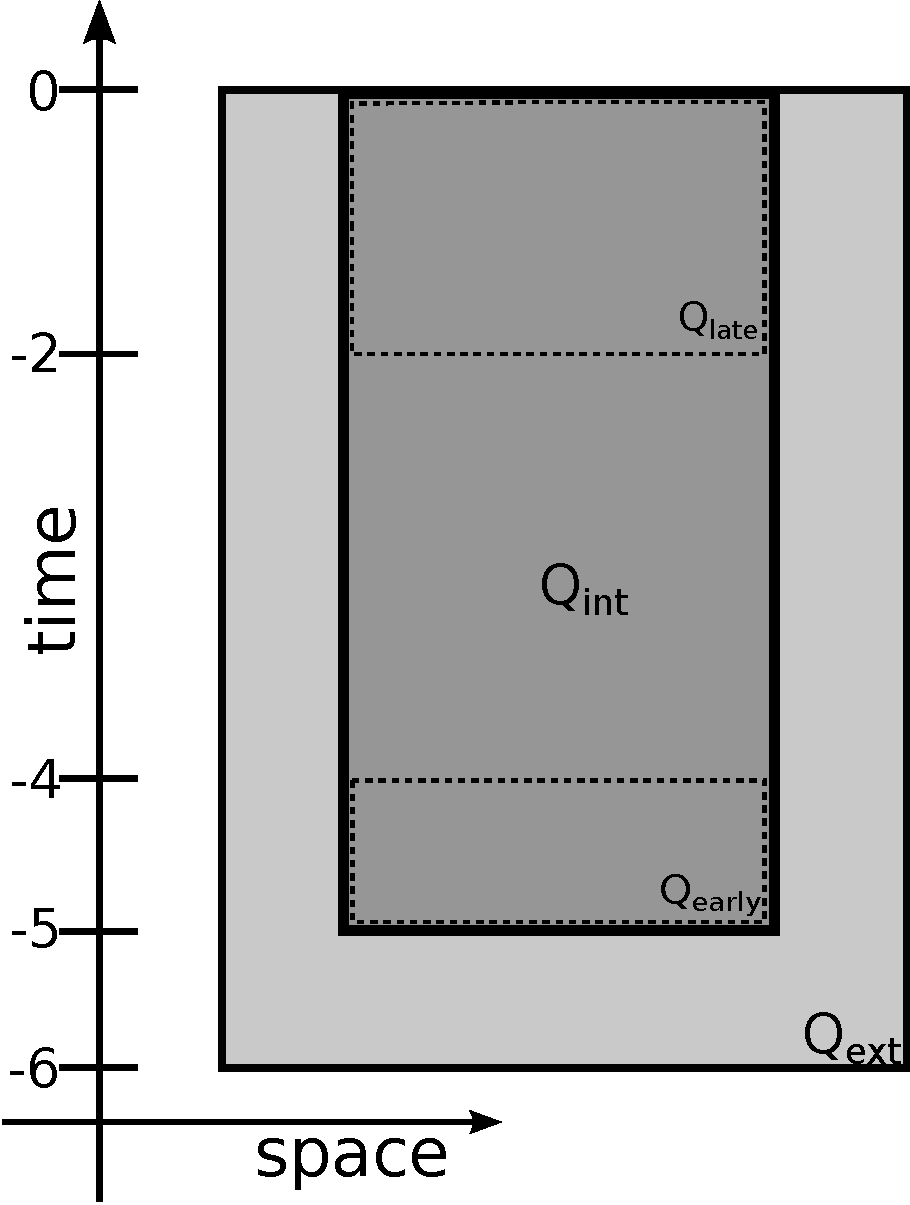
\includegraphics[width=.25 \textwidth]{NFP-diagram-Q-3}
\caption{Four overlapping cylinders described in Proposition~\ref{thm:DG2.kinetic}.}
\end{figure}

To state Proposition~\ref{thm:DG2.kinetic}, we must define four cylindrical regions in space-time:
\begin{align*} 
\Qext &:= [-6,0]\times B_3 \\
\Qint &:= [-5,0]\times B_2 \\
\Qearly &:= [-5,-4]\times B_2 \\
\Qlate &:= [-2,0]\times B_2. \\
\end{align*}

The constant $\delta_0$ in the statement of this proposition is defined in Proposition~\ref{thm:DG1.kinetic}.  

\begin{proposition}[Second De Giorgi Lemma]\label{thm:DG2.kinetic}
There exist universal constants $\gamma_0 > 0$ and $0 < \theta_0 < 1/3$ such that the following is true:

For any $f \in L^2(\Qext; H^s(\R^n))$ a weak solution to \eqref{eq:main.kinetic} subject to \eqref{eq:kappa_bound} with
\[ \norm{a}_{L^\sourceexp(\Qext \times \R^n)} \leq \theta_0 \]
satisfying
\[ |f(t,x,v)| \leq 1 + \psi_{\theta_0}(v) \qquad \forall (t,x,v) \in \Qext \times \R^n, \]
if
\begin{equation}\label{DG2_mass_early} 
|\{f \leq 0\} \cap \Qearly \times B_2| \geq \frac{|\Qearly| \cdot |B_2|}{2} 
\end{equation}
and
\begin{equation}\label{DG2_mass_late}
|\{f \geq 1-\theta_0 \} \cap \Qlate \times B_2| \geq \delta_0 
\end{equation}
then
\begin{equation}\label{DG2_mass_between}
|\{0 < f < 1-\theta_0 \} \cap \Qint \times B_3| \geq \gamma_0. 
\end{equation}
\end{proposition}

As in other applications of De Giorgi's method, the idea of the proof is to produce a sequence of solutions to our PDE with smaller and smaller intermediate measure, show that they are compact and have a discontinuous limit, and then show that said limit function inherits enough regularity from the PDE to result in a contradiction.  

Our version of the proof is divided into four steps.  In the first step, we show that our sequence is uniformly differentiable in $v$.  We then use the averaging lemma to show that, in some very specific sense, our sequence is uniformly differentiable in $t$ and $x$.  In the second step, we combine the results of step one to obtain compactness in all three variables, thus producing our limit.  In the third step, we show that this limit function is regular in $v$.  The limit is constant in $v$ for $|v|$ small, and behaves like an indicator function depending only on $t$ and $x$.  In the fourth and final step, we show that certain $t$- and $x$-derivatives of our limit function are bounded, and that this contradicts what we know about the jump discontinuities in our limit.  

\begin{proof}
Assume that the theorem is false.  Then there must exist a sequence $f_i$ of solutions to our equation \eqref{eq:main.kinetic} with operators $\L_i$ subject to \eqref{eq:kappa_bound} and source terms
\[ \norm{a_i}_{L^\sourceexp(\Qext \times \R^n)} \leq 1/i \]
such that 
\[ \abs{f_i(t,x,v)} \leq 1 + \psi_{1/i} \qquad \forall (t,x,v) \in \Qext \times \R^n \]
while
\begin{align*}
|\{f_i \leq 0\} \cap \Qearly \times B_2| &\geq \frac{|\Qearly|\cdot|B_2|}{2}, \\
|\{f_i \geq 1-\frac{1}{i} \} \cap \Qlate \times B_2| &\geq \delta_0, \\
|\{0 < f_i < 1-\frac{1}{i} \} \cap \Qint \times B_3| &\leq \frac{1}{i}.
\end{align*}
We wish to take a limit of these functions $f_i$.  


\step{Regularity in $v$ and regularity in $t,x$}%-----------%-----------%--------------%----------%----------%---------%_-----

Let $F:\R^n \to \R$ be a smooth radially-increasing function of $v$ which is identically $-1$ on $B_2$ and identically 0 outside of $B_3$.  Since $F \in \Ctest$, it is trivial to show that
\begin{equation}\label{LF_bounded} 
\norm{\L_i F}_\infty \leq C(n,s,\kappa). 
\end{equation}

\newcommand{\fip}{{f_i^+}}
\newcommand{\fim}{{f_i^-}}
To obtain compactness, we use a very blunt cutoff function $\bar{\psi}$ defined by
\begin{align*} 
\bar{\psi}(v) &:= \psi_\frac{1}{3}(v) + 1 + F(v), \\
\fip &:= \max\paren{f-\bar{\psi},0}, \\
\fim &:= \max\paren{\bar{\psi}-f,0}.
\end{align*}

Because $\psi_{1/3} \geq \psi_\theta$ for all $\theta < 1/3$ by Lemma~\ref{thm:psi_properties}, property \eqref{psi_increasing}, each $\fip$ for $i$ sufficiently large will be supported on $v \in B_3$.  In fact
\begin{equation}\label{f_leq_F} 
0 \leq \fip(t,x,v) \leq -F(v) \qquad \forall (t,x,v) \in \Qext \times \R^n. 
\end{equation}

Each $f_i$ is a solution to \eqref{eq:main.kinetic}, so we can apply Lemma~\ref{thm:energy_inequality} on the regions $\Qext$ and $\Qint$ with cutoff $\bar{\psi}$.   From \eqref{LF_bounded} and Lemma~\ref{thm:psi_properties}, property \eqref{L_of_psi} we know that $\norm{\L_i\bar{\psi}}_\infty$ is bounded by a finite universal constant.   The right hand side of this energy inequality is then universally bounded by \eqref{f_leq_F} so
\begin{equation}\label{Bs_are_bounded}
\iint_\Qint B_i(\fip,\fip) \,dxdt - \iint_\Qint B_i(\fip,\fim) \,dxdt \leq C(n,s,\kappa). 
\end{equation}
In particular, by Lemma~\ref{thm:B_and_Hs},
\begin{equation}\label{v_regularity_of_fip} 
\iint_\Qint \int \abs{\Lambda^s \fip}^2 \,dvdxdt \leq C(n,s,\kappa). 
\end{equation}
Critically, the constant $C(n,s,\kappa)$ does not depend on $i$.  

Unfortunately the energy inequality does not give us regularity in the $t$ and $x$ variables. In order to obtain compactness, therefore, we must rely on an averaging lemma.  To that end, apply the transport operator to $\fip^2$ and obtain
\begin{align*} 
\kinet \fip^2 &= 2 \fip \kinet f_i
\\ &= 2 \fip \L_i f_i + 2 \fip a_i
\\ &= 2 \fip \L_i\paren{f_i - \bar{\psi}} + 2 \fip \L_i \bar{\psi} + 2\fip a_i.
\end{align*}

For any function $g$ and operator $\L$ satisfying \eqref{eq:kappa_bound}, and $g_+ := \max(g,0)$, it is true that, for any $t$, $x$ fixed,
\begin{align*}
2 g_+ \L g &= \int 2 [g_+(v) g(w) - g_+(v)^2] K(t,x,v,w) \,dw
\\ &= \int [g_+(w)^2 - g_+(v)^2] K \,dw + \int [2 g_+(v) g(w) - g_+(v)^2 -  g_+(w)^2] K \,dw
\\ &= \int [g_+(w)^2 - g_+(v)^2] K \,dw - \int [g_+(w) - g_+(v)]^2 K \,dw + \int 2 g_+(v) [g(w) - g_+(w)] K \,dw
\\ &= \L g_+^2 - \int [g_+(w) - g_+(v)]^2 K \,dw - 2 \int g_+(v)g_-(w) K \,dw.
\end{align*}

Thus
\[ \kinet \fip^2 = H := H_1 + H_2 + H_3 + H_4 \]
where
\begin{align*} 
H_1 &:= \L_i \paren{\fip^2},
\\ H_2 &:= - \int [\fip(w) - \fip(v)]^2 K(v,w) \,dw,
\\ H_3 &:= - 2 \int \fip(v)\fim(w) K(v,w) \,dw,
\\ H_4 &:=  2 \fip \L_i \bar{\psi} + 2 \fip a_i.
\end{align*}

We proceed to bound $H$, term by term, independent of $i$.  

We begin with an $H^s$ bound on $\fip^2$:
\begin{align}
\int \abs{\Lambda^s (\fip^2)}^2 \,dv &= \iint \frac{|\fip^2(w)-\fip^2(v)|^2}{|v-w|^{n+2s}}\,dwdv \nonumber
\\ &= \iint \bracket{\fip(w)+\fip(v)}^2 \frac{|\fip(w)-\fip(v)|^2}{|v-w|^{n+2s}}\,dwdv \nonumber
\\ &\leq 2^2 \norm{\fip}_{L^\infty}^2 \int \abs{\Lambda^s (\fip)}^2 \,dv. \label{fip_in_Hs}
\end{align} 
From this, the bounds \eqref{f_leq_F} and \eqref{v_regularity_of_fip}, and Lemma~\ref{thm:B_and_Hs}, we obtain
\begin{equation}\label{bound_on_H1}
\norm{\bessel^{-s/2} H_1}_{L^2(\Qint\times\R^n)} \leq C(n,s,\kappa). 
\end{equation}

The terms $H_2$ and $H_3$ are strictly negative, so their total variations as measures are simply the absolute values of their integrals.  Thus their norms in $\mathcal{M}(\Qint \times \R^n)$ are
\[ \abs{\iint_{\Qint} \int H_2 \,dvdxdt} = \iint_{\Qint} B_i(\fip,\fip) \,dxdt, \]
\[ \abs{\iint_{\Qint} \int H_3 \,dvdxdt} = -\iint_{\Qint} B_i(\fip,\fim) \,dxdt. \]
%The existence of these bounds is the reason we are considering $\fip^2$ instead of $\fip$.  
These are of course universally bounded by \eqref{Bs_are_bounded}.  

Recall that $\paren{1-\Laplace_{v}}^{-\paren{s + \frac{n}{2}}/2}$ can be represented as convolution with a Green's function $G_{s+n/2}(v)$ (see e.g. Stein \cite{St.book}).  The function $G_{s+n/2}$ decays exponentially as $|v|\to \infty$ and has a singularity like $\frac{1}{|v|^{\frac{n}{2} - s}}$ near zero.  Therefore $G_{s+n/2}$ is in $L^2$.  By Young's Inequality, convolution of a measure and an $L^2$ function is bounded by the product of their $\mathcal{M}$ and $L^2$ norms respectively, so
\begin{equation}\label{bound_on_H2} 
\norm{\paren{1-\Laplace_v}^{-\paren{s + \frac{n}{2}}/2}H_2}_{L^2(\Qint \times \R^n)} \leq C(n,s,\kappa), 
\end{equation}
\begin{equation}\label{bound_on_H3}
\norm{\paren{1-\Laplace_v}^{-\paren{s + \frac{n}{2}}/2}H_3}_{L^2(\Qint \times \R^n)} \leq C(n,s,\kappa). 
\end{equation}

Lastly, from \eqref{f_leq_F} and since $\sourceexp \geq 2$ we know
\begin{equation}\label{bound_on_H4}
\norm{H_4}_{L^2(\Qint \times \R^n} \leq C(n,s,\kappa). 
\end{equation}

Finally we are ready to apply Lemma~\ref{thm:avg_lemma} to $\fip^2$, which says for any $\eta \in \Ctest(\R^n)$ and any subset $\bar{\Omega}$ compactly contained in the interior of $\Qext$,
\[ \norm{\int \eta \fip^2 \,dv}_{H^\alpha(\bar{\Omega})} \leq C(\eta, \bar{\Omega}) \paren{\norm{\fip^2}_{L^2(\Qint \times \R^n)} + \norm{\bessel^{-\paren{s + \frac{n}{2}}/2} H}_{L^2(\Qint\times\R^n)}} \]
%\norm{\int \eta f \,dv}_{H^\alpha(\bar{\Omega})} \leq C \paren{\norm{f}_{L^2(\Omega \times \R^n)} + \norm{\bessel^{-m/2} g}_{L^2(\Omega\times\R^n)}}. \]
where
\[ \alpha = \paren{2\paren{s+\frac{n}{2}}}\n. \]

From \eqref{bound_on_H1}, \eqref{bound_on_H2}, \eqref{bound_on_H3}, and \eqref{bound_on_H4}, we can say that in fact
\begin{equation}\label{Halpha_bounded} 
\norm{\int \eta \fip^2 \,dv}_{H^\alpha(\bar{\Omega})} \leq C(n,s,\kappa,\eta,\bar{\Omega}). 
\end{equation}

\step{Producing a strong $L^2$ limit}%-----------------%------------%---------------%---------------%-------------%-----------

Since all the $\fip$ are bounded by \eqref{f_leq_F}, $\{\fip^2\}_i$ is a bounded subset of $L^2(\Qint \times \R^n)$.  By Banach-Alaoglu, there exists a function $f^+$ such that, along some subsequence, 
\[ \fip^2 \weakly {f^+}^2 \]
weakly in $L^2(\Qint \times \R^n)$.  

Our goal is to show that this limit converges also strongly in $L^2_\loc(\Qint; L^2(\R^n))$.  To that end, fix some compact subset $\bar{\Omega}$ of $\Qint$.  

Strong and weak limits, when both exist, must be equal, so with the bound \eqref{Halpha_bounded} we apply Rellich-Kondrachov to prove that
\[ \int \eta(v) \fip^2 \,dv \to \int \eta(v) {f^+}^2 \,dv \]
strongly in $L^2(\bar{\Omega})$, without passing to a further subsequence, for any $\eta \in \Ctest(\R^n)$.  

In particular, if we fix some $\eta$ such that $\eta_\eps(v) = \eps^{-n} \eta(v/\eps)$ is an approximation to the identity, then for $\eps > 0$ and $v \in \R^n$ fixed,
\[ \iint_{\bar{\Omega}} \bracket{\int \fip^2(w) \eta_\eps(v-w) \,dw - \int {f^+}(w)^2 \eta_\eps(v-w) \,dw}^2 \,dxdt \xrightarrow{i\to\infty} 0. \]
Note that this is pointwise (in $v$) convergence of convolutions.

Since the $\fip$ are all bounded by \eqref{f_leq_F}, and by weak convergence so is ${f^+}$, we can apply the Lebesgue dominated convergence theorem to conclude that not only do these convolutions converge pointwise in $v$, but they converge in integral as well.  That is,
%\[ \int \iint_{\bar{\Omega}} \bracket{\int \fip^2(w) \eta_\eps(v-w) \,dw - \int \paren{{f^+}(w)}^2 \eta_\eps(v-w) \,dw}^2 \,dxdtdv \to 0. \]
\begin{equation}\label{convergence_of_convolutions}
\int \iint_{\bar{\Omega}} \bracket{\paren{\fip^2 \ast_v \eta_\eps}(v) - \paren{{f^+}^2 \ast_v \eta_\eps}(v)}^2 \,dxdtdv \to 0. 
\end{equation}

It is known (see Lemma~\ref{thm:convolution_estimate} in the appendix for a proof) that for any $g \in H^s(\R^n)$, 
\[ \norm{g - g\ast \eta_\eps}_{L^2(\R^n)} \leq C(n,s,\eta) \norm{g}_{H^s(\R^n)} \eps^s. \]

Therefore for our functions $\fip^2$, 
\[ \iint_{\bar{\Omega}} \int \paren{\fip^2 - \fip^s \ast_v \eta_\eps}^2 \,dvdxdt \leq C(n,s,\eta) \eps^{2s} \iint_\Qint \int |\Lambda^s \fip|^2 \,dvdxdt. \]

Remember that $\norm{\fip^2}_{L^2(\Qint;H^s(\R^n))}$ is bounded by \eqref{fip_in_Hs} and \eqref{v_regularity_of_fip}, and, since the $H^s$ norm is weakly lower-semi-continuous, $\norm{{f^+}^2}_{L^2(\Qint;H^s(\R^n))}$ will be bounded as well.  

Therefore we can bound
\begin{align*} 
\norm{\fip^2 - f_+^2}_2 &\leq \norm{\fip^2 - \eta_\eps \ast_v \fip^2}_2 + \norm{\eta_\eps \ast_v \fip^2 - \eta_\eps \ast_v {f^+}^2}_2 + \norm{{f^+}^2 - \eta_\eps \ast_v {f^+}^2}_2
\\ &\leq C \eps^s + \norm{\eta_\eps \ast_v \fip^2 - \eta_\eps \ast_v {f^+}^2}_2.
\end{align*}
By $\norm{\cdot}_2$ we mean $\norm{\cdot}_{L^2(\bar{\Omega}\times\R^n)}$.  For any $\delta > 0$, we take $\eps$ small enough that $C \eps^s \leq \delta/2$.  Then with $\eps$ fixed, we choose $i$ large enough that (by \eqref{convergence_of_convolutions}) $\norm{\eta_\eps \ast_v \fip^2 - \eta_\eps \ast_v {f^+}^2}_2 \leq \delta/2$.  This proves that $\norm{\fip^2 - f_+^2}_2$ goes to 0 as $i \to \infty$.  

Since this is true for any $\bar{\Omega}$ compactly contained in the interior of $\Qint$, we can say that $\fip^2 \to {f^+}^2$ in $L^2_\loc(\Qint;L^2(\R^n))$.  

In fact, since our domain is compact, this convergence happpens in $L^1_\loc(\Qint;L^2(\R^n))$ as well.  Since $\fip$ and $f_+$ are non-negative, and since $(x-y)^2 \leq \abs{x^2 - y^2}$ for any non-negative real numbers $x$ and $y$, we can say that
\[ \fip \to {f^+} \qquad \textrm{in } L^2_\loc(\Qint; L^2(\R^n)). \]


\step{The limit is constant in $v$}%-----%-----%-----%-----%-----%-----%-----%-----%-----%-----%-----%-----%-----%-----%-----

We'll denote 
\[ f = f^+ + 1 + F. \]

Because $\fip \to f^+$ strongly in $L^2_\loc$, we know that
\begin{equation}\label{mass_of_limit}
\begin{aligned}
|\{f = 0\} \cap \Qearly \times B_2| &\geq \frac{|\Qearly|\cdot|B_2|}{2}, \\
|\{f = 1 \} \cap \Qlate \times B_2| &\geq \delta_0, \\
|\{1+F < f < 1 \} \cap \Qint \times B_3| &= 0. 
\end{aligned}
\end{equation}

\begin{remark}
If $s \geq 1/2$, we can use the fact that the $H^s_v$ norm of $f$ is known to be finite for almost every $t,x$ fixed and obtain \eqref{constant_in_v} immediately, making the remainder of Step 3 unnecessary.  It is only in the case $s < 1/2$ that this regularity in $v$ is insufficient to rule out jump discontinuities.  Therefore we follow the technique used in \cite{CaChVa} and by Bass and Kassmann in \cite{BaKa} to exploit the energy inequality's cross term.  
\end{remark}

\newcommand{\flambda}{f_{i,\lambda}^+}
\newcommand{\flambdam}{f_{i,\lambda}^-}
For $0 < \lambda \ll 1$, define the functions
\begin{align*} 
\flambda &:= \paren{f_i - \psi_\lambda - 1 - \lambda F}_+, \\
\flambdam &:= \paren{f_i - \psi_\lambda - 1 - \lambda F}_-.
\end{align*}
%$f_{i,+} := \paren{f_i - \psi_\lambda - \lambda F}_+$ and $f_{i,-} := \paren{f_i - \psi_\lambda - \lambda F}_-$

From the the energy inequality of Lemma~\ref{thm:energy_inequality}, we see that for all $i$ the cross term is bounded
\begin{equation}\label{flambda_energy_inequality}
-\iint_\Qint B\paren{\flambda, \flambdam} \leq C(n,s,\kappa) \bracket{\iint_\Qext \int {\flambda}^2 + \sup_{v\in B_3} \L_i(\psi_\lambda + \lambda F) \iint_\Qext\int \flambda + \norm{a_i}_{\sourceexp} \norm{\flambda}_{\sourceexp^\ast}}. 
\end{equation}

For $v \in B_3$, Lemma~\ref{thm:psi_properties}, property \eqref{L_of_psi} says that $\L_i \psi_\lambda(v) \leq C_\psi \lambda^{3s/2}$.  Moreover by \eqref{LF_bounded}, $\abs{\L_i \lambda F(v)} \leq C\lambda$ for some universal constant $C$.  

For $\lambda$ fixed and $i$ sufficiently large, 
\[ f_i \leq 1+\psi_{1/i} \leq 1+\psi_\lambda \]
so
\[ 0 \leq \flambda \leq \lambda F. \]
Therefore, for $\lambda$ fixed and $i$ sufficiently large, the inequality \eqref{flambda_energy_inequality} yields
\[ \iint_\Qint -B\paren{\flambda, \flambdam} \leq C(n,s,\kappa) \bracket{\lambda^2 + (\lambda + \lambda^{3s/2})\lambda + (1/i)\lambda}. \]

%We produce a lower bound on the dissipation
The cross term in turn bounds the integral of $\flambda$ and $\flambdam$.  For any $t,x$ fixed
\begin{align*}
-B_i(\flambda, \flambdam) &= \iint K(v,w) \flambda(v) \flambdam(w) \,dwdv
\\ &\geq \frac{1}{\kappa} \iint_{|v-w| \leq 6} \frac{\flambda(v) \flambdam(w)}{|v-w|^{n+2s}} \,dwdv
\\ &\geq \frac{1}{\kappa} \iint_{|v|\leq 3, |w|\leq 3} \frac{\flambda(v) \flambdam(w)}{6^{n+2s}} \,dwdv
\\ &= C \int_{B_3} \flambda \,dv \int_{B_3} \flambdam \,dv.
\end{align*}

Since $f_i \to f$ strongly in $L^2_\loc(\Qint;L^2(\R^n))$, these upper- and lower-bounds on the cross term hold in the limit:
\begin{equation}\label{bound_on_good_term}
\iint_\Qint \bracket{ \int_{B_3} \paren{f-\psi_\lambda-1-\lambda F}_+ \,dv \int_{B_3} \paren{f-\psi_\lambda-1-\lambda F}_- \,dv} \,dxdt \leq C(n,s,\kappa) (\lambda^2 + \lambda^{1+3s/2}). 
\end{equation}

This bound on the limit $f$ is very strong, because by \eqref{mass_of_limit} we have either $f(t,x,v)=1$ or $f(t,x,v) = 1 + F(v)$ for almost all $(t,x,v) \in \Qint \times B_3$.  For such $(t,x,v)$, also $\psi_\lambda(v)=0$ and so
%\[ f-\psi_\lambda - 1 - \lambda F = \begin{cases} - \lambda F & f=1,
%\\ (1-\lambda) F & f = 1+F.
%\end{cases} \]
\[ f-\psi_\lambda - 1 - \lambda F = \bracket{-\lambda F} \indic{f=1	} + \bracket{(1-\lambda) F} \indic{f=1+F}. \]

The function $-\lambda F$ is non-negative, while $(1-\lambda)F$ is non-positive, so at any point $t,x \in \Qint$,
\begin{align*}
\int_{B_3} \paren{f-\psi_\lambda-1-\lambda F}_+ \,dv &= -\lambda \int F \indic{f=1} \,dv \\
\int_{B_3} \paren{f-\psi_\lambda-1-\lambda F}_- \,dv &= -(1-\lambda) \int F \indic{f=1+F} \,dv.
\end{align*} 

Plugging this into \eqref{bound_on_good_term} and moving all the $\lambda$ to one side, we obtain
\[ \iint_\Qint \int F \indic{f=1} \,dv \int F \indic{f=1+F} \,dv \,dxdt \leq C(n,s,\kappa) \frac{\lambda^2 + \lambda^{1+3s/2}}{\lambda(1-\lambda)}. \]
The left-hand side is independent of $\lambda$, and the right side tends to 0 as $\lambda \to 0$, so we conclude that the left-hand side is in fact 0.  In particular, this means that for almost every $t,x \in \Qint$, either
\begin{equation}\label{constant_in_v}
\abs{\{v: f(t,x,v) = 1\} \cap B_3 } = 0 \qquad \textrm{or} \qquad \abs{\{v: f(t,x,v) = 1+F\} \cap B_3 } = 0. 
\end{equation}


\step{The limit has bounded derivative, which is a contradiction}%-----%-----%-----%-----%-----%-----%-----%-----%-----%-----%-----%-----%-----%

What remains is to argue that $f$ increases from 0 to 1, without taking intermediate values along the way, despite having bounded derivative.  Moreover, it is not enough to bound the derivatives in any weak sense, because jump discontinuities can hide in sets of measure zero.  

Since $f$ is only defined up to an a.e.-equivalence class, we can assume without loss of generality that, for every (not a.e.) $t,x \in \Qint$, either $f(t,x,v) \equiv 1$ or $f(t,x,v) \equiv 1+F$.  

For each $i$, since $\bar{\psi}$ is constant in $t$ and $x$, it is true that
\[ \kinet\paren{f_i - \bar{\psi}} = \L_i \paren{f_i - \bar{\psi}} + \L_i\bar{\psi} + a_i. \]
Multiplying by $\indic{f_i \geq \bar{\psi}}$ and recalling the standard pointwise inequality for integral operators (c.f. \cite{CaSi.pointwise}),
\[ \kinet \fip \leq \L_i \fip + \indic{f_i \geq \bar{\psi}} \L_i\bar{\psi} + \indic{f_i \geq \bar{\psi}} a_i. \]

By \eqref{LF_bounded} and Lemma~\ref{thm:psi_properties}, property \eqref{L_of_psi}, the term $\indic{f_i \geq \bar{\psi}} \L_i\bar{\psi}$ is less than a universal constant $C(n,s,\kappa)$, and of course the $L^\sourceexp$ norm of $\indic{f_i \geq \bar{\psi}} a_i$ is less than $1/i$ so this term will vanish in the limit.  Let $\phi \in \Ctest(\Qint \times \R^n)$ be a non-negative test function and consider
\[ -\chevron{\fip, \kinet\phi} \leq \chevron{\fip, \L_i \phi} + \chevron{C, \phi} + \frac{1}{i} \norm{\phi}_{\sourceexp^\ast}. \]

For $\phi \in \Ctest$ fixed, the functions $\L_i \phi$ will be uniformly bounded in $L^\infty$ and decay like $|v|^{-n-2s}$.  In particular they are uniformly bounded in $L^2(\Qint \times \R^n)$.  Therefore
\[ \chevron{\fip - f^+, \L_i \phi} \to 0 \]
so in little-o notation
\[ -\chevron{\fip, \kinet\phi} \leq \chevron{\L_i f^+, \phi} + \chevron{C, \phi} + o(1). \]

%By Banach-Alaoglu, there exists a function we will call $\Phi$ such that $\L_i \phi \weakly \Phi$, at least along some subsequence.  Therefore in the limit
%\[ -\chevron{f^+, \kinet\phi} \leq \chevron{f^+, \Phi} + \chevron{C, \phi}. \]
%But remember that along the aforementioned subsequence,
%\begin{align*} 
%\chevron{f^+, \Phi} &= \lim \chevron{f^+,\L_i \phi}
%\\ &= \lim \chevron{\L_i f^+, \phi}. 
%\end{align*}

%Since in particular $\phi \in H^{2s+\eps}(\Qint\times\R^n)$ for some $\eps > 0$, the terms $\L_i \phi$ are uniformly bounded in $H^\eps$ for $\phi$ fixed so by Rellich-Kondrachov they have a strong $L^2$ limit which we can call $\Phi$, at least along some subsequence.  Therefore in the limit
%\[ -\chevron{f^+, \kinet\phi} \leq \chevron{f^+, \Phi} + \chevron{C, \phi}. \]
%But remember that along the aforementioned subsequence,
%\begin{align*} 
%\chevron{f^+, \Phi} &= \lim \chevron{f^+,\L_i \phi}
%\\ &= \lim \chevron{\L_i f^+, \phi}. 
%\end{align*}

By \eqref{constant_in_v} and \eqref{LF_bounded},
\[ \L_i f^+ = - \indic{t,x:f\equiv 1} \L_i F \leq C(n,s,\kappa). \]
Thus for some universal constant $C_1 = C_1(n,s,\kappa)$ we have, in the sense of distributions,
\[ \kinet \paren{f - 1 - F} \leq C_1. \]

%By taking the limit $f_i \to f$, in the sense of distributions, 
%\[ \kinet\paren{f-1-F}_+ \leq \L_i \paren{f-1-F}_+ + \L_i\bar{\psi}. \]
%But by \eqref{constant_in_v},
%\[ \L_i\paren{f-1-F}_+ = - \indic{t,x:f\equiv 1} \L_i F, \]
%which is a bounded function, so for some constant $C_1$ we have
%\[ \kinet \paren{f-1-F}_+ \leq C_1 \qquad \textrm{almost everywhere in } \Qint \times \R^n. \] 

To make the remaining calculation rigorous, let $\eta_\eps(t,x)$ be an approximation to the identity and define 
\[ f_\eps = \eta_\eps \ast_{t,x} f. \]
These functions $f_\eps$ are smooth and $f_\eps \to f$ pointwise a.e. as $\eps \to 0$.  For $(t,x)\in \Qint$ fixed, $f_\eps$, like $f$, is constant over all $v \in B_2$.  Because the transport operator commutes with convolution in $t$ and $x$,
\[ \kinet f_\eps = \eta_\eps \ast_{t,x} \kinet f \leq C_1. \]
This inequality is true not only in the sense of distributions but also pointwise because the functions are smooth.  

Define two sets
\begin{align*} 
M_1 &= \{t,x \in \Qlate: f(t,x,v) = 1 \}, \\
M_0 &= \{t,x \in \Qearly: f(t,x,v) = 1+F(v) \}. \\
\end{align*}
By \eqref{mass_of_limit} we know that $|M_0| \geq \frac{|\Qearly|}{2}$ and $|M_1| \geq \frac{\delta_0}{|B_2|}$.  By Egorov's theorem, for $\eps$ sufficiently small,
\begin{align}
|M_1^\eps| &:= \abs{\{t,x \in \Qlate: f_\eps(t,x,v) > 0.9 \, \forall v \in B_2\}} \geq \frac{\delta_0}{2|B_2|}, \label{size_of_M1eps} \\
|M_0^\eps| &:= \abs{\{t,x \in \Qearly: f_\eps(t,x,v) < 0.1 \, \forall v \in B_2\}} \geq \frac{|\Qearly|}{4}. \nonumber
\end{align}
Fixing $\eps$, choose a point $(t_0,x_0) \in M_0^\eps$.  


%By [cite mass assumptions], we know that there is at least one point $(t_0,x_0)$ in $\Qearly$ such that $f(t_0,x_0,v) = 0$ for all $v \in B_2$, and that the set of points $(t_1,x_1) \in \Qlate$ such that $f(t_1,x_1,v) = 1$ for all $v \in B_2$ has measure
%\[ \abs{\{t,x \in \Qlate: f(t,x,v) = 1 \}} \geq \frac{\delta_1}{|B_2|}. \]

For any $(t_1,x_1) \in M_1^\eps$, we can define the velocity $\bar{v} := \frac{x_1-x_0}{t_1-t_0}$ and see that $|\bar{v}| \leq 2$.  Then the function
\[ \tau \mapsto f_\eps\big((1-\tau)t_0 + \tau t_1, (1-\tau)x_0 + \tau x_1, \bar{v}\big) \]
is equal to 0 at $\tau = 0$ and equal to 1 at $\tau = 1$, and its derivative is less than $(t_1-t_0) C_1$.  Therefore
\begin{equation}\label{line_segments_have_large_measure}
\mathcal{H}^1\paren{\textrm{segment}\bracket{(t_0,x_0),(t_1,x_1)} \cap \{t,x: 0.1 < f(t,x,v) < 0.9 \, \forall v\in B_2\}} \geq \frac{.8 \sqrt{1 + |\bar{v}|^2}}{C_1} \geq \frac{2}{C_1}. 
\end{equation}

The facts \eqref{size_of_M1eps} and \eqref{line_segments_have_large_measure} tell us, by the elementary geometric argument of Lemma~\ref{thm:cone}, that the cone with vertex $(t_0,x_0)$ and base $M_1^\eps$ must intersect $\{t,x: 0.1 < f(t,x,v) < 0.9 \, \forall v\in B_2\}$ on a set with measure $(\delta_0/2|B_2|)(2/C_1)^2/80$.  

In particular,
\[ \abs{\{0.1<f_\eps<0.9\} \cap \Qint \times B_2} \geq \frac{2\delta_0}{80 C_1^2|B_2|} > 0. \]


This bound holds for all $\eps$ sufficiently small, but we know from \eqref{mass_of_limit} that it is not true for $f$.  By Egorov's theorem, this is a contradiction.  

Therefore our sequence $f_i$ must not exist, and the proposition must be true.  

\end{proof}






%-----%-----%-----%-----%-----%-----%-----%-----%-----%-----%-----%-----%-----%-----%-----%-----%-----%-----%

\section{H\"{o}lder Continuity}\label{sec:Holder}

In this section, we explain how Proposition~\ref{thm:DG1.kinetic} and Proposition~\ref{thm:DG2.kinetic} together lead to H\"{o}lder regularity of our solution.  We begin by showing that the PDE \eqref{eq:main.kinetic} is scaling invariant.  We then show, in Lemma~\ref{thm:oscillation}, how to combine Proposition~\ref{thm:DG1.kinetic} and Proposition~\ref{thm:DG2.kinetic} to create a sort of Harnack's inequality.  The ideas here are not new, in particular we follow \cite{CaChVa} very closely.  

\begin{lemma}[Scaling]\label{thm:scaling.kinetic}
If $f$ solves \eqref{eq:main.kinetic} on some region $Q\times \R^n \subseteq \Rall$, then for any constant $\eps < 1$, 
\[ \bar{f}(t,x,v) := f(\eps^{2s} t, \eps^{1+2s} x, \eps v) \]
will solve 
\[ \del_t \bar{f} + v \cdot \grad_x \bar{f} = \int [\bar{f}(w) - \bar{f}(v)] \bar{K}(t,x,v,w) \,dw + \bar{a} \]
on the appropriate region $Q_\eps\times\R^n$ with $\bar{K}$ symmetric and satisfying \eqref{eq:kappa_bound}, and with 
\[ \norm{\bar{a}}_{L^\sourceexp(Q_\eps\times\R^n)} \leq \eps^{2s\paren{1 - \frac{n+1+n/s}{\sourceexp}}} \norm{a}_{L^\sourceexp(Q\times\R^n)}. \]
\end{lemma}

\begin{proof}
Denote
\[ p = (t,x,v), \qquad \bar{p} = (\eps^{2s} t, \eps^{1+2s} x, \eps v). \]

Evaluate the equality \eqref{eq:main.kinetic} at the point $\bar{p}$, so that
\begin{equation}\label{PDE_at_barp}
(\del_t f)(\bar{p}) + \eps v \cdot (\grad_x f)(\bar{p}) = (\L f)(\bar{p}) + a(\bar{p}). 
\end{equation}

For our modified function $\bar{f}$ evaluated at $p$,
\begin{align} 
\del_t \bar{f}(p) &= \eps^{2s} (\del_t f)(\bar{p}), \label{scaled_delt} \\
\grad_x \bar{f}(p) &= \eps^{1+2s} (\grad_x f)(\bar{p}). \label{scaled_gradx}
\end{align}

Define
\[ \bar{K}(t,x,v,w) := \eps^{n+2s} K(\eps^{2s} t, \eps^{1+2s} x, \eps v, \eps w). \]
It's clear that $\bar{K}$ is still symmetric.  Since
\[ \bar{K}(t,x,v,w) \geq \eps^{n+2s} \indic{\eps |v-w| \leq 6} \frac{1}{\kappa} (\eps |v-w|)^{-(n+2s)} \geq \indic{|v-w| \leq 6} \frac{1}{\kappa} |v-w|^{-(n+2s)} \]
and 
\[ \bar{K}(t,x,v,w) \leq \eps^{n+2s} \kappa (\eps |v-w|)^{-(n+2s)} = \kappa |v-w|^{-(n+2s)}, \]
$\bar{K}$ satisfies the bound \eqref{eq:kappa_bound}.  

For this $\bar{K}$, 
\begin{align} 
\int [\bar{f}(w) - \bar{f}(v)] \bar{K}(p,w) \,dw &= \eps^{n+2s} \int [f(\eps w) - f(\eps v)] K(\bar{p}, \eps w) \,dw \nonumber
\\ &= \eps^{n+2s} \frac{1}{\eps^n} \int [f(\eps w) - f(\eps v)] K(\bar{p}, \eps w) \,d(\eps w) \nonumber
\\ &= \eps^{2s} (\L f)(\bar{p}). \label{scaled_L}
\end{align}

Define
\begin{equation}\label{scaled_sigma}
\bar{a}(t,x,v) := \eps^{2s} a(\eps^{2s} t, \eps^{1+2s} x, \eps v). 
\end{equation}
Then the $L^\sourceexp$ norm of $\bar{a}$ is
\[ \norm{\bar{a}}_\sourceexp = \eps^{2s} \eps^{-\frac{2s + n(1+2s) + n}{\sourceexp}} \paren{\iiint a(\eps^{2s} t, \eps^{1+2s} x, \eps v)^\sourceexp \,d(\eps^{2s} t)\, d(\eps^{1+2s} x) \, d(\eps v)}^{1/\sourceexp}. \]
%It is clear that this $\bar{a}$ satisfies the appropriate bound.  

Plugging \eqref{scaled_delt}, \eqref{scaled_gradx}, \eqref{scaled_L}, and \eqref{scaled_sigma} into \eqref{PDE_at_barp} yields
\[ \eps^{-2s} \del_t \bar{f}(p) + \eps \eps^{-1-2s} v\cdot\grad_x \bar{f}(p) = \eps^{-2s} \int [\bar{f}(w)-\bar{f}(v)] \bar{K}(p) \,dw + \eps^{-2s} \bar{a}(p). \]
Multiply both sides by $\eps^{2s}$ to obtain our desired result.  
\end{proof}

\begin{remark}
In addition to scaling, we can also translate solutions of \eqref{eq:main.kinetic}.  If $f$ is a solution and $(t_0,x_0,v_0)$ is a point in its domain, then
\[ \bar{f}(t,x,v) := f(t_0 + t, x_0 + x + v_0 t, v_0 + v) \]
will be a solution to \eqref{eq:main.kinetic} with similarly adjusted source term and kernel.  This translation invariance is necessary for the proof of H\"{o}lder continuity, though we omit any further detail.  
\end{remark}

The following lemma should be thought of as a Harnack inequality, except that it keeps track also of the growth in $v$.  

In the sequel, $\theta_0$ and $\gamma_0$ refer to the constant defined in the statement of Proposition~\ref{thm:DG2.kinetic}, and $\delta_0$ refers to the constant defined in Proposition~\ref{thm:DG1.kinetic} which is used again in the statement of Proposition~\ref{thm:DG2.kinetic}.

\begin{lemma}[Oscillation Lemma]\label{thm:oscillation}
There exists a universal constant $0 < \lambda < 1$ such that the following is true: 

If $f \in L^2(\Qext; H^s(\R^n))$ is a weak solution to \eqref{eq:main.kinetic} subject to \eqref{eq:kappa_bound} with source term
\[ \norm{a}_{L^\sourceexp(\Qext)} \leq \lambda \theta_0 \]
%\[ \norm{a}_{L^\infty(\Qext \times \R^n)} \leq \lambda \]
and satisfying
\begin{equation}\label{f_leq_1+psi}
|f(t,x,v)| \leq 1 + \lambda \psi_{\theta_0}(v) 
\end{equation}
for all $t,x \in \Qext$, $v \in \R^n$, then
\[ \bracket{\sup_{[-1,0]\times B_1 \times B_1} f} - \bracket{\inf_{[-1,0]\times B_1 \times B_1} f} \leq 2 - \lambda. \]

Moreover, at least one of the two functions
\[ \bar{f}_1(t,x,v) = \paren{1+\frac{\lambda}{2}}\bracket{f(\lambda^{2s} t, \lambda^{1+2s} x, \lambda v) + \lambda/2} \]
or
\[ \bar{f}_2(t,x,v) = \paren{1+\frac{\lambda}{2}}\bracket{f(\lambda^{2s} t, \lambda^{1+2s} x, \lambda v) - \lambda/2} \]
will also solve \eqref{eq:main.kinetic} subject to \eqref{eq:kappa_bound} in the weak sense with source term smaller than $\lambda \theta_0$ and satisfy 
\[ |\bar{f}_i(t,x,v)| \leq 1 + \lambda \psi_{\theta_0}(v) \]
for all $t,x \in \Qext$, $v \in \R^n$.  

%In particular, this means that 
%all the assumptions of lemma [oscillation] for at least one choice of $\pm$.  
%\[ \bracket{\sup_{[-1,0]\times B_1 \times B_1} f} - \bracket{\inf_{[-1,0]\times B_1 \times B_1} f} \leq 2 - \lambda. \]
\end{lemma}

\begin{proof}
Choose $k_0 \in \N$ such that
\[ \gamma_0 k_0 > |\Qint \times B_3|. \]
Take $\lambda$ small enough that
\begin{equation}\label{lambda_assumptions}
\lambda \leq \frac{\theta_0^{k_0+1}}{2}, \qquad 3\lambda^{1+2s} < 1, \qquad 6\lambda^{2s} < 1, \qquad \lambda < \eps_0, \qquad \textrm{ and } \paren{1+\frac{\lambda}{2}}\lambda^{2s\paren{1 - \frac{n+1+n/s}{\sourceexp}}} \leq 1
\end{equation}
where $\eps_0 = \eps_0(s,\theta_0)$ is defined in Lemma~\ref{thm:psi_properties} property \eqref{psi_scaled_inequality}.  

Assume without loss of generality that 
\begin{equation} \label{fk_can_haz_measure_below}
|\{f\leq 0\} \cap \Qearly \times B_2| \geq |\Qearly|\cdot |B_2|/2. 
\end{equation}  
If this were not true, then we could simply discuss $-f$ instead.  This proposition holds for $f$ if and only if it holds for $-f$.  

With this assumption, we will assert that the proposition's result is true for
\[ \bar{f}(t,x,v) = \paren{1+\frac{\lambda}{2}}\bracket{f(\lambda^{2s} t, \lambda^{1+2s} x, \lambda v) + \lambda/2}. \]
It is clear by Lemma~\ref{thm:scaling.kinetic} and linearity of Equation~\eqref{eq:main.kinetic} that $\bar{f}$ will solve \eqref{eq:main.kinetic} subject to \eqref{eq:kappa_bound} with source term $\bar{a}$ smaller than $\lambda \theta_0$ by \eqref{lambda_assumptions}.  We must show that $\bar{f}$ is also bounded as desired.  

Consider the sequence of functions
\begin{align*}
f_0 &= f \\
f_k &= \frac{f_{k-1}-1}{{\theta_0}} + 1 = \frac{f-1}{{\theta_0}^k} + 1.
\end{align*}
Since equation~\eqref{eq:main.kinetic} is linear, all $f_k$ will also be solutions with source terms $\frac{1}{\theta_0^k} a$.  

For each $0 \leq k \leq k_0+1$ and any $(t,x,v) \in \Qext\times\R^n$, 
\[ |a(t,x,v)| \leq \frac{\lambda\theta_0}{\theta_0^k} \leq \theta_0 \]
by the assumption \eqref{lambda_assumptions}, and by \eqref{f_leq_1+psi} and \eqref{lambda_assumptions},
\begin{equation}\label{fk_has_bounded_growth} 
f_k = \frac{f-1}{{\theta_0}^k} + 1 \leq \frac{\lambda}{{\theta_0}^k} \psi_{\theta_0} + 1 \leq \psi_{\theta_0} + 1. 
\end{equation}

We wish to show that $f_{k_0}$ satisfies
\begin{equation}\label{fk_can_haz_DG1}
|\{f_{k_0} \geq 1-{\theta_0}\}\cap \Qlate \times B_2| \leq \delta_0. 
\end{equation}
Therefore assume, for contradiction, that \eqref{fk_can_haz_DG1} does not hold.  Then by construction, each $f_k$ will satisfy \eqref{DG2_mass_late} for $0 < k \leq k_0$.  Moreover, all $f_k$ will satisfy \eqref{DG2_mass_early} since $f_0$ does by \eqref{fk_can_haz_measure_below}.  Therefore we can apply Proposition~\ref{thm:DG2.kinetic} and conclude that each $f_k$ for $k$ from 0 to $k_0$ must satisfy \eqref{DG2_mass_between}.  That means that the set
\[ S_k := |\{f_k \leq 0\} \cap \Qint \times B_3| \]
must increase in measure by at least $\gamma_0$ with each increment of $k$.  By choice of $k_0$, this would be a contradiction.  We conclude that \eqref{fk_can_haz_DG1} holds.  
%\[ |\{f_{k_0} \geq 1-{\theta_0}\}\cap [-2,0]\times B_2 \times B_2| \leq \delta_0. \]

Due to \eqref{fk_has_bounded_growth} and Lemma~\ref{thm:psi_properties}, property \eqref{psi_geq_one_plus_psi}, we say that for all $t,x \in \Qlate$ and all $|v| \geq 2$
\[ f_{k_0+1}(t,x,v) \leq 1 + \psi_{\theta_0}(v) \leq \psi^1(v). \]
By \eqref{fk_has_bounded_growth}, $f_{k_0+1}(t,x,v) \leq 1$ for all $(t,x,v) \in [-2,0]\times B_2 \times B_2$, so we can say by \eqref{fk_can_haz_DG1} that
%Therefore by \eqref{fk_can_haz_DG1} for all $(t,x,v) \in \Qlate \times B_2$,
\[ \iiint_{\Qlate \times B_2} \max(f_{k_0+1}-\psi^1,0)^2 \,dvdxdt \leq \delta_0. \]

This is sufficent to apply Proposition~\ref{thm:DG1.kinetic} to $f_{k_0+1}$ and conclude that $ f_{k_0+1} \leq 1/2$ on $[-1,0]\times B_1 \times B_1$.  Thus for the original $f$,
\begin{equation}\label{Harnack_partial_result} 
-1 \leq f \leq 1-\frac{1}{2} {\theta_0}^{k_0+1} \leq 1-\lambda \qquad \forall (t,x,v)\in [-1,0]\times B_1 \times B_1. 
\end{equation}
This proves the lemma's first claim.  

We now know from \eqref{Harnack_partial_result}, the definition of $\bar{f}$, and \eqref{lambda_assumptions} that for all $t,x \in \Qext$ and $|v| \leq \lambda\n$
\begin{align*}
\bar{f}(t,x,v) &\leq \paren{1+\frac{\lambda}{2}} \bracket{ 1 - \lambda + \lambda/2} \leq 1, \\
\bar{f}(t,x,v) &\geq \paren{1+\frac{\lambda}{2}} \bracket{-1 + \lambda/2} \geq -1.
\end{align*}

For $t,x \in \Qext$ and $|v| \geq \lambda\n$, since $\lambda < \eps_0$, we know by Lemma~\ref{thm:psi_properties}, property \eqref{psi_scaled_inequality} that
\[ 2 \psi_{\theta_0}(\lambda v) + 2 \leq \psi_{\theta_0}(v). \]
Therefore
\begin{align*} 
\abs{\bar{f}(t,x,v)} &\leq \paren{1 + \frac{\lambda}{2}} \bracket{1 + \lambda \psi_{\theta_0}(\lambda v) + \lambda/2} 
\\ &\leq \paren{1 + \frac{\lambda}{2}} \bracket{1 + \frac{\lambda}{2} \psi_{\theta_0}(v) - \lambda + \lambda/2} 
%\\ &= \paren{1 - \frac{\lambda^2}{4}} + \paren{\frac{\lambda}{2} + \frac{\lambda^2}{4}} \psi_{\theta_0}(v)
%\\ &\leq 1 + \frac{\lambda}{2-\lambda} \bracket{\psi_{\theta_0}(v)-2}
\\ &\leq 1 + \lambda \psi_{\theta_0}(v).
\end{align*}

This completes the proof.  

\end{proof}

%In particular, this means that for any integer $k$, in the space-time-velocity region
%\[ [-h^{2sk}, 0] \times B_{h^{(1+2s)k}} \times B_{h^k} \]
%one expects $f$ to lie between $C-\paren{\frac{2-\lambda}{2}}^k$ and $C+\paren{\frac{2-\lambda}{2}}^k$, for some constant $C$.  By applying this fact 
%
%The H\"{o}lder exponent is 
%\[ \log\paren{\frac{2-\lambda}{2}} \big/ \log(h). \]
%$r^{\log(v-w)/\log(h)} = |v-w|^{\log(r)/\log(h)}$.  
%
%Done with oscillation, time for oscillation-plus-scaling.  Should probably combine these.  
%
%\begin{lemma}
%Let $f$ satisfy the assumptions of lemma [oscillation].  Let $h > 0$ be a small constant satisfying
%\[ 3h^{1+2s} \leq 1, \qquad 6h^{2s} \leq 1, \qquad \textrm{ and } \qquad h < \eps_0. \]
%
%The scaled function
%\[ \bar{f}(t,x,v) = \frac{2}{2-\lambda}\bracket{f(h^{2s} t, h^{1+2s} x, h v) \pm \lambda/2} \]
%will also satisfy all the assumptions of lemma [oscillation] for at least one choice of $\pm$.  
%\end{lemma}
%
%\begin{proof}
%By lemma [scaling] and the fact our PDE is linear, this new function $\bar{f}$ will satisfy \eqref{eq:main.kinetic}.  
%
%Apply lemma [oscillation] to $f$, and without loss of generality, for $t,x,v \in [-1,0]\times B_1 \times B_1$
%\[ f(t,x,v) \leq 1-\lambda. \]
%By choice of $h$, for all $t,x \in \Qext$ and $|v| \leq 1/h$,
%\[ -1 = \frac{2}{2-\lambda} \bracket{1 + \lambda/2} \leq \bar{f}(t,x,v) \leq \frac{2}{2-\lambda} \bracket{ 1 - \lambda + \lambda/2} = 1. \]
%
%For $t,x \in \Qext$ and $|v| \geq 1/h$, since $h < \eps_0$, we know that
%\[ 2 \psi_{\theta_0}(hv) + 2 \leq \psi_{\theta_0}(v). \]
%Therefore
%\begin{align*} 
%\abs{\bar{f}(t,x,v)} &\leq \frac{2}{2-\lambda} \bracket{1 + \lambda \psi_{\theta_0}(hv) + \lambda/2} 
%\\ &\leq 1 + \frac{\lambda}{2-\lambda} \bracket{\psi_{\theta_0}(v)-2}
%\\ &\leq 1 + \lambda \psi_{\theta_0}(v).
%\end{align*}
%
%\end{proof}

Theorem~\ref{thm:main} is proven by iteratively applying this Lemma~\ref{thm:oscillation} to an appropriately scaled function.  

%------------------%---------------------%--------------------%------------------%_--------------%-------------------%_----

\appendix
\section{Some Technical Lemmas}\label{sec:appendix}
%\appendix

We prove here the averaging lemma used throughout this paper.  
This lemma is an immediate corollary of \cite{Be} Theorem 6.  It is merely a localization of that result.  
\begin{lemma}[Averaging Lemma]\label{thm:avg_lemma}
Let $\Omega$ be an open subset of space-time $\R \times \R^n$, and $\bar{\Omega}$ a compact subset of $\Omega$.  

For any smooth function $\eta \in \Ctest(\R^n)$ and any $m \in \R^+$, there exists a constant $C = C(n,m,\eta, \bar{\Omega}, \Omega)$ and a constant
\[ \alpha = \frac{1}{2(1+m)} \]
such that the following is true:

For any two functions $f$ and $g$ in $L^2(\Omega \times \R^n)$ satisfying
\[ \kinet f = g, \]
it is true that
\[ \norm{\int \eta f \,dv}_{H^\alpha(\bar{\Omega})} \leq C \paren{\norm{f}_{L^2(\Omega \times \R^n)} + \norm{\bessel^{-m/2} g}_{L^2(\Omega\times\R^n)}}. \]
%
%Assume that
%\[ \kinet f = g. \]
%Then for any smooth function $\eta \in \Ctest(\R^n)$ and any $m \in \R^+$, there exists a constant $C = C(n,m,\eta, \bar{\Omega}, \Omega)$ and a constant
%\[ \alpha = \frac{1}{2(1+m)} \]
%such that
%\[ \norm{\int \eta f \,dv}_{H^\alpha(\bar{\Omega})} \leq C \paren{\norm{f}_{L^2(\Omega \times \R^n)} + \norm{\bessel^{-m/2} g}_{L^2(\Omega\times\R^n)}}. \]
\end{lemma}

By $\norm{g}_{H^\alpha(\bar{\Omega})}$, we mean the infimum of $\norm{\tilde{g}}_{H^\alpha(\R^{n+1})}$ over all extensions $\tilde{g}$ of $g$ to $\R^{n+1}$.  

\begin{proof}
Let $\phi(t,x)$ be a smooth function supported on $\Omega$ and identically equal to 1 on $\bar{\Omega}$.  Then
\[ \kinet (\phi f) = \phi g + f \kinet \phi. \]
By \cite{Be} Theorem 6,
\[ \norm{\phi \int \eta f \,dv}_{H^\alpha(\R \times \R^n)} \leq C \paren{\norm{\phi f}_{L^2(\R \times \R^n \times \R^n)} + \norm{\bessel^{-m/2} \paren{\phi g + f \kinet \phi}}_{L^2(\R \times \R^n \times \R^n)}}. \]
Because $\bessel^{-m/2}$ is a bounded operator from $L^2$ to $L^2$, and because $\phi$ is a smooth function supported on $\Omega$ and depending only on $t$ and $x$, 
\[ \norm{\bessel^{\frac{-m}{2}} \paren{\phi g + f \kinet \phi}}_{L^2(\R^{1+n+n})} \leq C(\phi) \norm{\bessel^{\frac{-m}{2}}g}_{L^2(\Omega\times \R^n)} + C(m,\phi)\! \norm{f}_{L^2(\Omega\times\R^n)}\!. \]

The result follows.  
\end{proof}

The following is a technical lemma about the geometry of cones.  We use it at the very end of the proof of Proposition~\ref{thm:DG2.kinetic}.  

\begin{figure}[h]
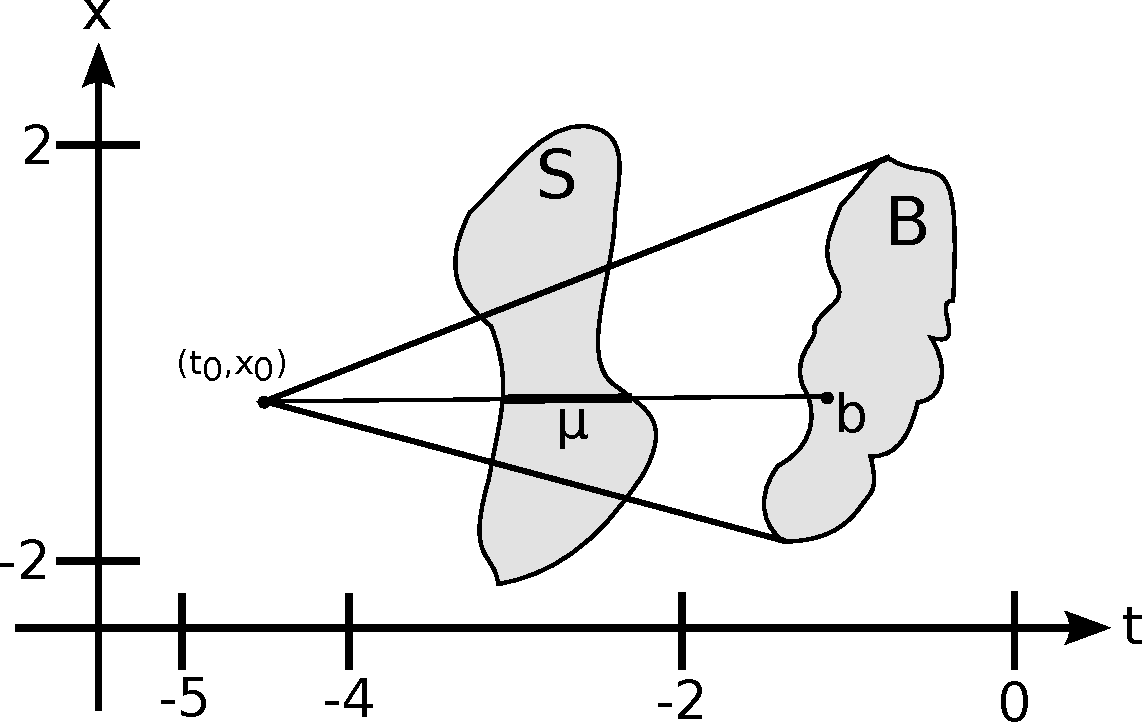
\includegraphics[width=.5 \textwidth]{NFP-diagram-Cone}
\caption{A diagram showing the assumptions of Lemma~\ref{thm:cone}.}
\end{figure}

\begin{lemma}\label{thm:cone}
Let $\mathcal{C} \subseteq \R \times \R^n$ be a cone from a vertex $(t_0,x_0) \in [-5, -4] \times B_2$ to a base set $B \subseteq [-2,0]\times B_2$.  % having $(t_0,x_0) \in [-5, -4] \times B_2$ and $B \subseteq [-2,0]\times B_2$.  
Let $S$ be a subset of $\R\times\R^n$ such that for each $b \in B$, the line segment connecting $(t_0,x_0)$ to $b$ intersects $S$ on a set with Hausdorff $\mathcal{H}^1$ measure at least $\mu$.  

Then 
\[ \abs{\mathcal{C} \cap S} \geq \frac{ |B| \mu^2}{80}. \]
\end{lemma}

\begin{proof}
Let $A(t)$ be the cross-sectional area of our cone at time slice $t$.  If $\mathcal{H}^n$ is the Hausdorff measure of dimension $n$, we write
\[ A(t) = \mathcal{H}^n\paren{\mathcal{C} \cap \bracket{\{t\}\times \R^n}}. \]
By the nature of cones, $A(t_0)=0$, $A$ is affine for $t_0 < t < -2$, then sub-affine for $-2<t<0$, and $A(t)=0$ for $t > 0$.  Specifically,
\[ A(t) = \frac{A(-2)}{-2-t_0} \paren{t-t_0} \qquad t_0 < t < -2, \]
\[ A(t) \leq \frac{A(-2)}{-2-t_0} \paren{t-t_0} \qquad -2 \leq t. \]


Since $B$ is contained in $\mathcal{C} \cap [-2,0]\times \R^n$, 
\[ |B| \leq \int_{-2}^0 A(t) \,dt \leq \int_{-2}^0 \frac{A(-2)}{-2-t_0}\paren{t-t_0} \,dt = \frac{A(-2)}{-2-t_0} \bracket{t_0^2 - (2+t_0)^2}/2 \leq 4 A(-2). \]

This means that 
\[ A(-2) \geq \frac{|B|}{4}. \]

Now we have a lower bound on the size of the cone, so for $t_0 \leq t \leq -2$
\begin{equation}\label{lower_bound_on_A} 
A(t) \geq \frac{|B|}{4(-2-t_0)}(t - t_0). 
\end{equation}

%Since $A(t)$ is increasing in $t$, the total measure of $\mathcal{C}\cap S$ will be smallest when $S$ is located near the vertex.  Each segment intersects $S$ on a set with measure at least $\mu$, and a segment of length $\mu$ can fit inside the cylinder $[t_0,t_0+x]\times B_2$ $\mu^2 = 4^2 + x^2$, $x = \sqrt{\mu^2 - 16}$.  At its most slant, a segment goes up $-2-t_0$ and over $4$, so with an extent $t$ you get rise $t$ and run $4t/(-2-t_0)$ for a length$^2$ of $t^2 + 16t^2/(2+t_0)^2$ or $t^2 \paren{1 + 16/2^2} = 5t^2$.  
%
%Consider a point $b \in B$ and the line segment from $(t_0,x_0)$ to $b$, which intersects $S$ on a set of measure at least $\mu$.  Because $A(t)$ is increasing in $t$, this intersection contributes more 

Consider the map from $B$ to $\{0\}\times\R^n$ given by stereographic projection from the point $(t_0,x_0)$, and let $db$ be a probability measure on $B$ proportional to the pullback of $\mathcal{H}^n \rest_{\{0\}\times\R^n}$ under this projection.  %In other words, $db(E)$ is the probabilty that a ray from $(t_0,x_0)$ to $B$ will intersect $E$.  
%Let $db$ be a probability measure on $B \subseteq \R \times \R^n$ which is a pullback of the stereographic projection, with pole $(t_0,x_0)$, from $\R \times \R^n$ to a copy of $\R^n$.  It measures what percentage of the rays from $(t_0,x_0)$ intersect a region of $B$.  
Then $db$ represents the proportion of any time-slice of $\mathcal{C}$ generated by rays through a given portion of $B$.  

To find the measure of $\mathcal{C} \cap S$, we must ask how much each time slice intersects $S$, or in integral form
\[ \abs{\mathcal{C} \cap S} = \int_{t_0}^{0} A(t) \int_{b \in B} \indic{(t,x) \in \mathcal{C} \cap S} \,dbdt. \]
By Fubini, this becomes
\begin{equation}\label{measure_of_intersection} 
\abs{\mathcal{C} \cap S} = \int_{b \in B} \int_{t_0}^0 A(t) \indic{(t,x) \in \mathcal{C} \cap S} \,dtdb. 
\end{equation}

From the definition of $\mu$ and the arc length formula,
\[ \mu \leq \int_{t_0}^0 \indic{(t,x) \in \mathcal{C} \cap S} \sqrt{1 + |b-x_0|^2/(-2-t_0)^2} \,dt \leq \sqrt{5} \int_{t_0}^0 \indic{(t,x) \in \mathcal{C} \cap S}. \]

Because $A(t)$ is increasing and $\indic{(t,x) \in \mathcal{C} \cap S}$ integrates to at least $\mu/\sqrt{5}$, 
\[ \int_{t_0}^0 A(t) \indic{(t,x) \in \mathcal{C} \cap S} \,dt \geq \int_{t_0}^{t+\mu/\sqrt{5}} A(t) \,dt. \]
From this bound, \eqref{measure_of_intersection}, and \eqref{lower_bound_on_A} we can at last compute
\[ \abs{\mathcal{C} \cap S} \geq \frac{|B|}{4(-2-t_0)} \int_{t_0}^{t_0 + \mu/\sqrt{5}} (t-t_0) \,dt = \frac{|B|}{4(-2-t_0)} \frac{\mu^2}{10} \geq \frac{|B|\mu^2}{80}. \]
\end{proof}

The following lemma is a commonly known fact about mollifiers.  Despite being known, a proof is surprisingly difficult to find in the existing literature.  Therefore, in the interest of completeness, we prove it here.   

\begin{lemma}\label{thm:convolution_estimate}
Let $\eta\in \Ctest(\R^n)$ be such that the sequence $\eta_\eps(v) = \eps^{-n} \eta(v/\eps)$ is an approximation to the identity.  There exists a constant $C=C(n,s,\eta)$ such that, for any $g \in H^s(\R^n)$, 
\[ \norm{g - g\ast \eta_\eps}_{L^2(\R^n)} \leq C \norm{g}_{H^s(\R^n)} \eps^s. \]
\end{lemma}

\begin{proof}
The bound is easy to compute by taking the Fourier transform and using Plancharel's theorem:
\begin{align*} 
\norm{g - g\ast \eta_\eps}_{L^2}^2 &= \int \hat{g}^2 \paren{1 - \hat{\eta_\eps}}^2 \,d\xi 
\\ &\leq \int (1+\xi^2)^s \hat{g}^2 \,d\xi \,\, \sup_{\xi} \frac{\abs{1-\hat{\eta_\eps}(\xi)}^2}{(1+\xi^2)^s}
\\ &= \norm{g}_{H^s(\R^n)}^2 \,\, \sup_{\xi} \frac{\abs{1-\hat{\eta_\eps}(\xi)}^2}{(1+\xi^2)^s}.
\end{align*}

Since $\eta \in \Ctest$, the fourier transform $\hat{\eta}$ is Lipschitz with some constant $\bar{C}$. Thus $\hat{\eta_\eps}(\xi) = \hat{\eta}(\eps \xi)$ is Lipschitz with constant $\bar{C}\eps$.  Since $\eta_\eps$ is an approximation to the identity, $\hat{\eta_\eps}(0) = 1$ and $\abs{\hat{\eta_\eps}(\xi)} \leq 1$ for all $\xi$.  Thus
\[ \abs{1 - \hat{\eta_\eps}(\xi)} \leq \min(2,\bar{C}\eps|\xi|). \]
%
%Our goal is to bound
%\begin{align*} 
%\norm{g - g\ast \eta_\eps}_{L^2}^2 &= \int \hat{g}^2 \paren{1 - \hat{\eta_\eps}}^2 \,d\xi 
%\\ &\leq \int (1+\xi^2)^s \hat{g}^2 \frac{\min(2,C\eps|\xi|)^2}{(1+\xi^2)^s} \,d\xi. 
%\end{align*}

The function $\frac{\min(2,\bar{C}\eps\xi)^2}{(1+\xi^2)^s}$ achieves its maxumum value at the critical point $\bar{C}\eps|\xi| = 2$, and that maximum value is 
\[ \frac{2^2}{\paren{1+\paren{\frac{2}{\bar{C}\eps}}^2}^s} = \frac{4 \eps^{2s}}{\paren{\eps^2 + 4/\bar{C}^2}^s} \leq C \eps^{2s}. \]
\end{proof}

%\bibliographystyle{plain}
%\bibliography{NFP-references.bib}
%
%\end{document}

\chapter{SQG} \label{ch:SQG}

%\documentclass[11pt]{amsart}
%\usepackage{amssymb,amsbsy,upref,epsf,MnSymbol}
%\usepackage{amsmath,amssymb,amsthm}
%\usepackage{graphicx,mathtools,mathrsfs,wrapfig}
%\usepackage[margin=1in]{geometry}
%\usepackage{fancyhdr}
%\usepackage{enumerate}
%%\usepackage{enumitem}
%
%
%
%%-------------------------------------------<commands>--------------------------------------------------------
%\newtheorem{theorem}{Theorem}[section]
%\newtheorem{proposition}[theorem]{Proposition}
%\newtheorem{lemma}[theorem]{Lemma}
%\theoremstyle{remark}
%\newtheorem*{remark}{Remark}
%\theoremstyle{definition}
%\newtheorem{definition}{Definition}
%%%%%%%%%%%%%%%%%%%%%%%%%%%%%%%%%%%%%%%%%%
%\newcommand{\R}{\mathbb{R}}
%\newcommand{\N}{\mathbb{N}}
%\newcommand{\Z}{\mathbb{Z}}
%\newcommand{\Q}{\mathbb{Q}}
%\newcommand{\C}{\mathbb{C}}
%\newcommand{\Prj}{\mathbb{P}}
%\newcommand{\F}{\mathbb{F}}
%\newcommand{\A}{\mathbb{A}}
%\newcommand{\Four}{\mathcal{F}}
%\newcommand{\T}{\mathbb{T}}
%\newcommand{\E}{\mathcal{E}}
%\renewcommand{\L}{\mathcal{L}}
%\newcommand{\eps}{\varepsilon}
%%%%%%%%%%%%%%%%%%%%%%%%%%%%%%%%%%%%%%%%%%
%\newcommand{\floor}[1]{\left\lfloor #1 \right\rfloor}
%\newcommand{\ceil}[1]{\left\lceil #1 \right\rceil}
%\newcommand{\chevron}[1]{\langle #1 \rangle}
%\newcommand{\norm}[1]{\left\lVert#1\right\rVert}
%\newcommand{\paren}[1]{\left( #1 \right)}
%\newcommand{\bracket}[1]{\left[ #1 \right]}
%\newcommand{\abs}[1]{\left\lvert #1 \right\rvert}
%%%%%%%%%%%%%%%%%%%%%%%%%%%%%%%%%%%%%%%%%%
%\DeclareMathOperator{\id}{id}
%\DeclareMathOperator{\convex}{conv}
%\DeclareMathOperator{\image}{Im}
%\DeclareMathOperator{\im}{Im}
%\DeclareMathOperator{\coker}{coker}
%\DeclareMathOperator{\supp}{supp}
%\DeclareMathOperator{\trace}{tr}
%\DeclareMathOperator{\lspan}{span}
%\DeclareMathOperator{\conv}{conv} % stands for conv, as in convex hull
%\DeclareMathOperator{\Int}{int} % stands for int, as in interior of a set
%\DeclareMathOperator{\sign}{sign}
%\DeclareMathOperator{\ran}{ran}
%\DeclareMathOperator{\rank}{rank}
%%\DeclareMathOperator{\dim}{dim}
%\newcommand{\dom}{\operatorname{dom}}
%\newcommand{\cod}{\operatorname{cod}}
%\newcommand{\Hom}{\operatorname{hom}}
%\newcommand{\Ob}{\operatorname{Ob}}
%\newcommand{\cl}{\operatorname{cl}}
%\DeclareMathOperator{\BMO}{BMO}
%%%%%%%%%%%%%%%%%%%%%%%%%%%%%%%%%%%%%%%%%%%
%\newcommand{\del}{\partial}
%\newcommand{\pvec}[2]{\frac{\partial #1}{\partial #2}}
%\newcommand{\grad}{\nabla}
%\newcommand{\ddt}{\frac{d}{dt}}
%\renewcommand{\div}{\operatorname{div}}
%\newcommand{\Laplace}{\Delta}
%\newcommand{\kinet}{\bracket{\del_t + v\cdot \grad_x}}
%\newcommand{\bessel}{\paren{1-\Laplace_v}}
%\newcommand{\loc}{\text{loc}}
%\newcommand{\Lip}{\text{Lip}}
%%\newcommand{\BMO}{\text{BMO}}
%\renewcommand{\Re}{\operatorname{Re}}
%\newcommand{\ddz}{\frac{d}{dz}}
%%%%%%%%%%%%%%%%%%%%%%%%%%%%%%%%%%%%%%%%%%%
%\newcommand{\into}{\hookrightarrow}
%\newcommand{\onto}{\twoheadrightarrow}
%\newcommand{\isom}{\cong}
%\newcommand{\rest}{{\upharpoonright}}
%\newcommand{\weakly}{\rightharpoonup}
%%%%%%%%%%%%%%%%%%%%%%%%%%%%%%%%%%%%%%%%%%%
%\newcommand{\ith}{^\mathrm{th}}
%\newcommand{\n}{^{-1}}
%\newcommand{\half}{\frac{1}{2}}
%%%%%%%%%%%%%%%%%%%%%%%%%%%%%%%%%%%%%%%%%%%
%\newcommand{\indic}[1]{\chi_{\{#1\}}}
%%%%%%%%%%%%%%%%%%%%%%%%%%%%%%%%%%%%%%%%%%%
%
%
%\newcommand{\eigen}[1]{\eta_{#1}} %my eigenfunctions
%\newcommand{\Ctest}{C_c^\infty}
%\newcommand{\test}{\mathcal{D}}
%
%\newcommand{\ulow}{u_\ell}
%\newcommand{\uhigh}{u_h}
%\newcommand{\ulowth}[1]{\ulow^{#1}}
%\newcommand{\uhighth}[1]{\uhigh^{#1}}
%
%\newcommand{\Gammal}{\Gamma_\ell}
%
%\newcommand{\HD}{\mathcal{H}}
%\newcommand{\HDint}[2]{\int \abs{\Lambda^{#1} #2}^2}
%\newcommand{\HDinth}[1]{\HDint{1/2}{#1}}
%
%\newcommand{\Ccalib}{\kappa}
%\newcommand{\Cgamma}{C_\mathit{pth}}
%\newcommand{\Comega}{C_\mathit{dmn}}
%\newcommand{\Csuit}{C^\ast}
%
%\newcommand{\Rom}[1]{\MakeUppercase{\romannumeral #1}}
%
%\newcounter{step_count}[section]
%\newcommand{\step}[1]{\stepcounter{step_count} \smallskip \noindent{\textbf{Step \arabic{step_count}:} #1}}
%
%
%%-------------------------------------------</commands>--------------------------------------------------------
%
%%\newcommand{\draftnum}{1}%-----------------------------UPDATE DRAFT NUM----------------------------------------
%
%\title[Boundary Regularity for SQG]{Holder regularity up to the boundary for critical SQG on bounded domains}
%
%\author[Stokols]{Logan F. Stokols} 
%\address[L. F. Stokols]{\newline Department of Mathematics, \newline The University of Texas at Austin, Austin, TX 78712, USA}
%\email{lstokols@math.utexas.edu}
%
%\author[Vasseur]{Alexis F. Vasseur}
%\address[A. F. Vasseur]{\newline Department of Mathematics, \newline The University of Texas at Austin, Austin, TX 78712, USA}
%\email{vasseur@math.utexas.edu}
%
%\date{\today}
%
%\subjclass[2010]{35Q35,35Q86}
%%Logan: think about keyword for Japanese thing
%\keywords{SQG, Bounded domain, Besov spaces on bounded domains, H\"older regularity,  De Giorgi method}
%
%\thanks{\textbf{Acknowledgment.} This work was partially supported by the NSF Grant DMS 1614918 and the NSF RTG Grant DMS 1840314. 
%We would also like to thank the referee for suggesting several improvements to the paper, especially the construction of global suitable solutions.}
%
%\begin{document}
%
%\begin{abstract}
%We consider the dissipative SQG equation in bounded domains, first introduced by Constantin and Ignatova in 2016. 
%We show global Holder regularity up to the boundary of the solution, with a method based on the De Giorgi techniques. The boundary introduces several difficulties. In particular, the Dirichlet Laplacian is not translation invariant near the boundary, which leads to complications involving the Riesz transform.
%
%%We show global Holder regularity up to the boundary of the solution. 
%
%%The method is based on the De Giorgi techniques as in the 2010 work of Caffarelli and V. The boundary introduces several difficulties, as the Dirichlet Laplacian is not translation invariant near the boundary which makes the Riesz transform poorly behaved.  
%% lack of translation invariance of the Laplacian operator, or the fact that the gradient does not commute with the Dirichlet Laplacian. 
%\end{abstract}
%
%
%\maketitle \centerline{\date}
%
%\tableofcontents

\section{Preliminaries} \label{preliminaries}
The surface quasigeostrophic equation (SQG) is a special case of the quasi-geostrophic system (QG) with uniform potential vorticity. The QG model is used extensively in meteorology and oceanography (e.g. Charney \cite{Ch}). These models are described in Pedlosky \cite{Pe}. The SQG model was popularized by Constantin, Majda and Tabak in \cite{CoMaTa}, due to its similarities with the Euler and Navier-Stokes  equation. They proposed it as a toy model for the study of 3D Fluid equations (see also Held, Garner, Pierrehumbert, and Swanson \cite{GaHePiSw}). 

\vskip0.3cm
 We consider in this chapter critical SQG on a bounded domain. We will focus on the following model, which was introduced by Constantin and Ignatova in \cite{CoIg.fraclap} and \cite{CoIg.sqg}.
 Consider  $\Omega$ a connected bounded domain in $\R^2$ with $C^{2,\beta}$ boundary for some $\beta \in (0,1)$, and the Laplacian with homogeneous Dirichlet boundary conditions $-\Laplace_D$.  If $(\eigen{k})_{k \in \N}$ is the sequence of $L^2$-normalized eigenfunctions of $-\Laplace_D$ with corresponding eigenvalues $\lambda_k$ listed in non-decreasing order, define
\[ \Lambda f := \sum_{k=0}^\infty \sqrt{\lambda_k} \chevron{f,\eigen{k}}_{L^2(\Omega)} \eigen{k}. \]
The critical SQG problem on $\Omega$ with initial data $\theta_0 \in L^2(\Omega)$ is
\begin{equation} \label{eq:main nonlinear} \begin{cases}
\del_t \theta + u\cdot \grad \theta + \Lambda \theta = 0 & (0,T) \times \Omega,
\\ u = \grad^\perp \Lambda\n \theta & [0,T] \times \Omega,
\\ \theta = \theta_0 & \{0\} \times \Omega.
\end{cases} \end{equation}

In the model, the dissipation $\Lambda =\paren{-\Delta_D}^{1/2}$  is due to the  Ekman pumping, while the nonlinear velocity $u$ comes from the geostrophic and hydrostatic balance (see \cite{Pe}).
\vskip.3cm

The main result of this chapter is the following:
\begin{theorem} \label{thm:main continuity}
There exists a universal constant $C_1 > 0$ such that the following holds:

For any $\Omega \subseteq \R^2$ open and bounded with $C^{2,\beta}$ boundary, $\beta \in (0,1)$, there exists for any $S > 0$ a constant $C_S > 0$ (depending also on $\Omega$), and for any $k > 0$ a constant $\alpha_{k,S} \in (0,1)$ (depending also on $\Omega$) so the following holds:
\vskip.3cm

For any $\theta_0 \in L^2(\Omega)$ there exists a global-in-time weak solution $\theta \in L^\infty([0,\infty);L^2(\Omega)) \cap L^2([0,\infty);\HD^{1/2})$ to \eqref{eq:main nonlinear} verifying $\theta(t,x) = 0$ on $(0,\infty)\times \del\Omega$ and $\lim_{t \to 0} \theta(t,\cdot) = \theta_0$ in the $L^2$-weak sense.  For $k \geq \norm{\theta_0}_{L^2(\Omega)}$ and for every $S > 0$
\[ \theta \in C^{\alpha_{k,S}}([S,\infty)\times\bar{\Omega}) \]
where $\bar{\Omega}$ denotes the closure of $\Omega$.  

Moreover,
\[ \norm{\theta}_{L^\infty([S,\infty)\times\bar{\Omega})} \leq \frac{C_1}{S} \norm{\theta_0}_{L^2(\Omega)} \]
and
\[ \norm{\theta}_{C^{\alpha_{k,S}}([S,\infty)\times\bar{\Omega})} \leq C_S \norm{\theta_0}_{L^2(\Omega)}. \]

%Let $\Omega \subseteq \R^2$ be a bounded open set with $C^{2,\beta}$ boundary, $\beta \in (0,1)$, and let $\bar{\Omega}$ denote the closure of $\Omega$.  
%\vskip.3cm
%
%For any $\theta_0 \in L^2(\Omega)$, there exists a global-in-time weak solution $\theta \in C^\alpha((0,\infty)\times \bar{\Omega})$ to \eqref{eq:main nonlinear} which verifies $\theta(t,x) = 0$ on $(0,\infty) \times \del\Omega$ and verifies $\lim_{t \to 0} \theta(t,\cdot) = \theta_0$ in the $L^2$-weak sense.  
%
%Moreover, there exists a universal constant $C_1$ such that, for any time $t > 0$,
%\[ \norm{\theta}_{L^\infty([t,\infty)\times\bar{\Omega})} \leq \frac{C_1}{t} \norm{\theta_0}_{L^2(\Omega)} \]
%and there exists a constant $\alpha \in (0,1)$ depending only on $t$, $\Omega$, and $\norm{\theta_0}_{L^2(\Omega)}$ and a constant $C_2$ depending on $t$ and $\Omega$ such that
%\[ \norm{\theta}_{C^\alpha([t,\infty)\times\bar{\Omega})} \leq C \norm{\theta_0}_{L^2(\Omega)}. \]

%Let $T > t$ be a time, and $\theta_0 \in L^2(\Omega)$ with $\norm{\theta_0}_{L^2} \leq K$, and $\bar{\Omega}$ the closure of $\Omega$.  If $\theta$ and $u$ are a suitable weak solution to \eqref{eq:main nonlinear} on $[0,T] \times \Omega$ with initial data $\theta_0$, then $\theta$ is bounded and H\"{o}lder continuous in time and space uniformly on $(t,T)\times\bar{\Omega}$.  
%\vskip0.3cm
%
%More precisely, 
%\[ \norm{\theta}_{L^\infty([t,T]\times\bar{\Omega})} \leq C \norm{\theta_0}_{L^2(\Omega)} \]
%and 
%\[ \norm{\theta}_{C^\alpha([t,T]\times\bar{\Omega})} \leq C \norm{\theta_0}_{L^2(\Omega)}. \]
%
%\vskip.3cm
%
%Moreover, any weak solution $\theta \in L^\infty(0,T; L^2(\Omega)) \cap L^2(0,T; H_0^1(\Omega))$ to \eqref{eq:main nonlinear} and corresponding $u$ will be a suitable pair.  

%More precisely, there exists $\alpha \in (0,1)$ depending only on $\Omega$ and $\norm{\theta_0}_{L^2(\Omega)}$, and some constant $C$ depending only on $\Omega$ and $t$, such that
%\[ \norm{\theta}_{C^\alpha((t,T)\times\Omega)} \leq C \norm{\theta_0}_{L^2(\Omega)}. \]
\end{theorem}

This model was first thoroughly studied in the cases without boundaries (either $\R^2$ or the torus $\T^2$).   
Global weak solutions were first constructed in Resnick \cite{Re}. Global regularity was first shown with small initial values by Constantin, Cordoba, and Wu \cite{CoCoWu}, or extra $C^\alpha$ regularity on the velocity in Constantin and Wu \cite{CoWu} and Dong and Pavlovi\'{c} \cite{DoPa}. In \cite{KiNaVo}, Kiselev, Nazarov and Volberg showed the 
propagation of $C^\infty$ regularity. The global $C^\infty$ regularity for any $L^2$ initial values was first proved in  \cite{CaVa.sqg} (see also Kiselev and Nazarov \cite{KiNa.variations} and Constantin and Vicol \cite{CoVi}).   

\vskip0.3cm

In the presence of boundaries, there are several  distinct ways to define SQG. This can be attributed  to alternative generalizations of the fractional Laplacian.  Kriventsov \cite{Kr.landsea} considered a two-phase problem which satisfies critical SQG only in part of the domain, and was able to prove H\"{o}lder regularity in the time-independent case.  This problem, intended to model air currents over a region containing both land and water, contains a half-Laplacian and a Riesz transform defined, not spectrally, but in terms of extension.  In \cite{NoVa.bounded}, the authors consider the Euler-Coriolis-Boussinesq model and derive the full 3D inviscid quasigeostrophic system in an impermeable cylinder (see also \cite{NoVa.solutions} for the construction of small time smooth solutions to the model).  They obtain natural boundary conditions for SQG distinct from the homogeneous conditions introduced in \cite{CoIg.fraclap}, \cite{CoIg.sqg} and described above. 
However, due to the complexity of the model described in \cite{NoVa.bounded}, we focus in this chapter only on the homogenous case.

\vskip0.3cm
Existence of weak solutions for \eqref{eq:main nonlinear}  is proven in \cite{CoIg.fraclap}, and local existence and uniqueness for strong solutions with sufficiently smooth initial data is proven by Constantin and Nguyen in \cite{CoNg.strong} (see also Constantin and Nguyen \cite{CoNg} and Constantin, Ignatova, and Nguyen \cite{CoIgNg} for the inviscid case). The interior regularity of solutions  is proven in \cite{CoIg.sqg} (together with propagation of $L^\infty$ bounds).  The method of proof for interior regularity uses  nonlinear maximum principles, introduced by Constantin and Vicol \cite{CoVi}.   However, the bounds obtained in \cite{CoIg.sqg} blow up near the boundary and do not provide global regularity.
  In \cite{CoIg.sqg} Remark 1, questions about   global regularity are suggested as  open problems.  Both the $C^\alpha(\bar{\Omega})$ regularity,  and bootstrapping to  $C^\infty(\bar{\Omega})$ regularity, are indentified as interesting problems.  
  Our  result answers the first question, by  showing  that solutions $\theta$ to (\ref{eq:main nonlinear}) are globally H\"{o}lder continuous.
  Bootstrapping to $C^\infty$ involves different techniques, and will be studied in a forthcoming work \cite{StVa.higher}.  
\vskip0.3cm

Our proof is based on  the De Giorgi method pioneered by De Giorgi in \cite{DG}.  The method was applied to the SQG problem first in \cite{CaVa.sqg}.  The method is powerful for showing $C^\alpha$ regularity of elliptic- and parabolic-type equations. It has been applied in a variety of situations for non-local problems, such as the fractional heat equation in \cite{CaChVa.nio}, the time-fractional case in \cite{AlCaVa}, the 3D Quasigeostrophic problem in \cite{NoVa.qg}, or the kinetic setting by Imbert and Silvestre \cite{ImSi} or in \cite{St.hypo}.  The method has also been applied in more exotic, non-elliptic situations such as Hamilton-Jacobi equations (see \cite{ChVa}, \cite{StVa.hamjac}).  

The De Giorgi method involves rescaling our equation by zooming in iteratively, and applying regularity results at each scale.  Therefore it is important that certain results be proven independently of the domain $\Omega$.  
%In particular, $\Omega$, like $\theta$ and $u$, will throughout this paper refer to a general object which may not match the assumptions of Theorem~\ref{thm:main continuity}.  
The particular dependence on $\Omega$ will be made clear in each lemma of this chapter.  
As a general overview, in the proof of Theorem~\ref{thm:main continuity} we will apply the results of Sections~\ref{sec:suitable} and \ref{sec:littlewood paley} only on a single fixed domain, while the results of Sections~\ref{sec:de giorgi} and \ref{sec:harnack} must be applied at each level of zoom with a different rescaled domain each time.  
%, as a general overview, the results of Sections~\ref{sec:Linfty} and \ref{sec:littlewood paley} will be applied, in the proof of Theorem~\ref{thm:main continuity}, only at the first level (hence their results may depend strongly on $\Omega$), while the results of Sections~\ref{sec:de giorgi} and \ref{sec:harnack} must be applied at each level of zoom with a different domain each time.  

% is assumed throughout throughout this paper to be a completely arbitrary domain unless otherwise specified.  
\vskip0.3cm

The first broad  idea of our proof consists in decoupling the  velocity $u$ from  $\theta$ to work on  a linear equation, and prove alternating regularity results for $\theta$ and $u$ independently.  We can show that $\theta$ is in $L^\infty$ without any assumption on $u$ (see Section~\ref{sec:suitable}).  
Using that $L^\infty$ bound, we will need to obtain scaling invariant controls on the drift   $u = \grad \Lambda^{-1} \theta$.  By scaling invariant, we mean that the bound, once proven on $\Omega$ fixed, will remain true of the scaled function $u(\eps \, \cdot, \eps \, \cdot)$ for all $\eps$.  
Unfortunately, although the Riesz transform is bounded from $L^p$ to $L^p$ for all $p$ finite, it is not bounded for $p = \infty$.  
The usual technique, therefore, is to consider $\BMO$ (as in \cite{CaVa.sqg} and \cite{NoVa.qg}), but in the case of bounded domains the Riesz transform is not known to be bounded in this space either.  Our solution is to use extensions of the Littlewood-Paley theory to bounded domains. 

The adaptation of Fourier analysis and Littlewood-Paley theory to Schrodinger operators is a well-studied subject (e.g. Zheng \cite{Zh}, Benedetto and Zheng \cite{BeZh}).  As an application of this theory, Iwabuchi, Matsuyama, and Taniguchi \cite{IMT.besov}, \cite{IMT.schrodinger}, and Bui, Duong, and Yang \cite{BuDuYa} have considered operators defined on open subsets of $\R^n$, which includes as a special case the operator $-\Laplace_D$ (a Schrodinger operator with zero potential).  In particular, in \cite{IMT.bilinear},  Iwabuchi, Matsuyama, and Taniguchi derive many important results, including the Bernstein inequalities, for Besov spaces adapted to the operator $-\Laplace_D$ on bounded open subsets of $\R^n$ with smooth boundary.  This theory turns out to greatly improve our understanding of the Riesz transform $\grad \Lambda^{-1}$ on bounded domains.  


Using the results of \cite{IMT.bilinear}, we will be able to show that the Riesz transform of an $L^\infty$ function whose Fourier decomposition $f = \sum f_k \eigen{k}$ is supported on high frequencies $k > N$ will be bounded in the weak sobolev space $W^{-1/4,\infty}$, and the Riesz transform of an $L^\infty$ function whose Fourier decomposition is supported on low frequencies $k<N$ will have bounded Lipschitz constant.  The cutoff $N$ for dividing high frequencies from low frequencies must depend however on the size of the domain $\Omega$.  In the case of $\R^2$, where $\grad$  and $\Lambda^{-1}$ commute, this is equivalent to the observation that the Riesz transform is bounded from $L^\infty$ to the Besov space $B_{\infty,\infty}^0$.  In the case of bounded domains, the argument must be more subtle.  We must decompose $\theta$ into its Littlewood-Paley projections, individually bound the Riesz transform of each projection in multiple spaces, and then recombine these infinitely-many functions into a low-frequency collection and a high-frequency collection depending on the scale of oscillation we are trying to detect (see Section~\ref{sec:littlewood paley} and Lemma~\ref{thm:calibration is good}).  

We make this notion precise with the following definition:

\begin{definition}[Calibrated sequence] \label{def:calibrated}
Let $\Omega\subseteq \R^2$ be any bounded open set and $0<T\in\R$.  We call a function $u\in L^2([0,T]\times\Omega)$ \textbf{calibrated} if it can be decomposed as the sum of a calibrated sequence 
\[ u = \sum_{j \in \Z} u_j \]
with each $u_j \in L^2([0,T]\times\Omega)$ and the infinite sum converging in the sense of $L^2$.  

We call a sequence $(u_j)_{j\in\Z}$ \textbf{calibrated} for a constant $\Ccalib$ and a center $N$ if each term of the sequence satisfies the following bounds.  
\begin{align*}
\norm{u_j}_{L^\infty([0,T]\times\Omega)} &\leq \Ccalib, \\
\norm{\grad u_j}_{L^\infty([0,T]\times\Omega)} &\leq 2^{j} 2^{-N} \Ccalib, \\
\norm{\Lambda^{-1/4} u_j}_{L^\infty([0,T]\times\Omega)} &\leq 2^{-j/4} 2^{N/4} \Ccalib.  
\end{align*} 

\end{definition}
\vskip.3cm

In Section \ref{sec:holder} we will show that a calibrated velocity remains calibrated at all scales (specifically, with fixed constant $\Ccalib$ but a changing center $N$).  Therefore we can consider, for any domain $\Omega$ and time $T$, the system of linear equations
\begin{equation} \label{eq:main linear} \begin{cases}
\del_t \theta + u \cdot \grad \theta + \Lambda \theta = 0, & [-T,0]\times\Omega \\
\div u = 0 & [-T,0]\times\Omega.
\end{cases} \end{equation}

In Section \ref{sec:suitable} we show that solutions to \eqref{eq:main nonlinear} with $L^2$ initial data exist and regularize instantly into $L^\infty$, and in Section~\ref{sec:littlewood paley} we show that the Riesz transform of $L^\infty$ data is calibrated.  Then in Sections \ref{sec:de giorgi} and \ref{sec:harnack} we will show that solutions to \eqref{eq:main linear} with calibrated velocity have decreasing oscillation between scales.  By iteratively applying this oscillation lemma and scaling our equation, we show in Section~\ref{sec:holder} that $\theta$ is H\"{o}lder continuous.  
\vskip.3cm

The low-freqency component of a calibrated velocity $u$ will be uniformly Lipschitz, which means it is only bounded up to a constant.  This is similar to the case of BMO velocity functions in \cite{CaVa.sqg} and \cite{NoVa.qg}, which by the John-Nirenberg inequality are also bounded up to a constant.  As in these cases, we consider a moving reference frame, denoted $\Gamma:[0,T] \to \R^2$, in which our velocity is shifted by a constant, making the low-frequency component of $u$ bounded. There are two differences between our implementation of this technique and the implementation in \cite{CaVa.sqg} and \cite{NoVa.qg}: firstly, we subtract off the value of the low-frequency part of $u$ at a point, rather than subtracting off the average of $u$ on a ball.  Secondly, rather than applying the standard De Giorgi argument to $\tilde{\theta}(t,x) := \theta(t,x+\Gamma(t))$, we must reformulate the De Giorgi argument to ``follow'' the path $\Gamma(t)$ explicitly.  This is a purely notational difference, but it is necessary because otherwise $\Omega$ would be time-dependent.  
%Unlike in previous instances of this method which subtract off the average of $u$ on a ball, we subtract off the value of the low-frequency part of $u$ at a point.  Previously, given a path $\Gamma$, they replace $\theta(t,x)$ by $\theta(t,x+\Gamma(t))$ and show regularization for this new function.  This is only possible in a homogenous domain.  Since we study the case with boundary, we cannot make this change of coordinates by $\Gamma$ implicit, and instead we will show that $\theta$ regularizes for $|x-\Gamma(t)|$ small.  
%
%Another difference is that while previous instances use a coordinate transformation to include their moving reference frame into the definition of $\theta$ at each scale, we make our moving frame explicit by showing that $\theta$ regularizes near a path $\Gamma$.  This is because such a coordinate transformation would lead to 
% This moving reference frame has no effect on the De Giorgi argument so long as the shifting frame is the same at each scale; our decrease-of-oscillation lemma will have both its assumptions and its conclusions phrased in terms of the same moving frame so the proof is unaffected.  

At each scale, there will be a natural Lagrangian path $\Gammal$ corresponding to the low-frequency part of $u$.  However, the low-frequency part of $u$ changes non-trivially as we zoom, so $\Gammal$ will be different at each scale.  Throughout Sections~\ref{sec:de giorgi} and \ref{sec:harnack}, we will use $\Gammal$ to denote the ``current'' Lagrangian path and $\Gamma$ to denote the Lagrangian path at the previous scale. In the proof of Theorem~\ref{thm:main continuity} in Section~\ref{sec:holder}, these are denoted $\Gamma_k(t)$ and $\eps\n \Gamma_{k-1}(\eps t)$ respectively.  In Lemmas~\ref{thm:energy inequality}, \ref{thm:DG1}, \ref{thm:DG2} and \ref{thm:oscillation general}, we will make assumptions about $\theta$ which are centered on $x \approx \Gamma(t)$ and obtain conclusions which are similarly centered on $x \approx \Gamma(t)$, conditioned on $\gamma := \Gammal-\Gamma$ being small in Lipschitz norm.  Finally in Lemma~\ref{thm:oscillation shifted}, we will show that, given bounds on $\theta$ for $x \approx \Gamma(t)$, we can bound $\theta$ for $x \approx \Gammal(t)$ for $t$ sufficiently small, again conditioned on $\gamma := \Gammal-\Gamma$ being small in Lipschitz norm.  Controlling $\gamma$ amounts to controlling the change in $\Gammal$ between consecutive scales, which is much easier to obtain than scale-independent bounds on $\Gammal$.  
% 
% The part of our moving reference frame which is maintained from the previous scale will be encoded by a function $\Gamma(t)$\footnote{In \cite{CaVa.sqg} and \cite{NoVa.qg}, the same technique is used.  However, there $\Gamma$ is not written explicitly, instead they perform a change of coordinates.  Though notationally this is cleaner, it only works in the full domain $\R^2$.  To avoid a time-dependent domain, we must write $\Gamma$ explicitly in each lemma.  This is a purely notational hurdle, the mathematical substance is unchanged.}.  That said, the reference frame associated to the low-frequency component of $u$ will change slightly at each scale, because the cutoff between low-frequency and high-frequency (i.e. the center of calibration) is scale-dependent.  However, we will easily show that the change in velocity is uniformly small.  The part of our moving reference frame which is novel at the current scale will be encoded by a function $\gamma(t)$.  The precise construction is in Section~\ref{sec:holder} in the proof of Theorem~\ref{thm:main continuity}.  
%
%By ``moving reference frame,'' we mean that instead of proving a decrease-in-oscillation between cylinders $[0,T]\times B_R(0)$ and $[T/2,T]\times B_r(0)$, we will prove a decrease-in-oscillation between tubular regions $\{(t,x)|t \in [0,T], x\in B_R(\Gamma(t))\}$ and $\{(t,x)|t \in [T/2,T], x\in B_r(\Gamma(t) + \gamma(t))\}$.  The precise argument is in Section~\ref{sec:harnack}.  
\vskip.3cm

Previous applications of the De Giorgi method to non-local equations such as \eqref{eq:main linear} generally make extensive use of either an extension representation (c.f. \cite{CaVa.sqg}) or a singular integral representation (c.f. \cite{NoVa.qg}).  In this chapter, we  use the singular integral representation for the Dirichlet fractional Laplacian  derived by Caffarelli and Stinga \cite{CaSt}. It is based on the results of Stinga and Torrea \cite{StTo} which generalize the extension representation of Caffarelli and Silvestre \cite{CaSi.extension}. 
This theory is pivotal in translating the existing non-local De Giorgi techniques to the problem at hand (see Section~\ref{sec:lambda}).  
\vskip.3cm

In order to apply De Giorgi's method to weak solutions of \eqref{eq:main linear}, we will need to assume a certain a priori estimate which holds, in particular, for $L^2(H_0^1)$ weak solutions.  However, such solutions are only known to exist for short time and for $H^2$ initial data, as shown by Constantin and Nguyen in \cite{CoNg.strong}.  We call weak solutions in $L^2(\HD^{1/2})$ which happen to verify this a priori estimate ``suitable solutions,'' by analogy to suitable solutions to Navier-Stokes as in \cite{CaKoNi}.  We give the formal definition of suitable solutions in Section~\ref{sec:suitable}, where we also construct global-in-time suitable solutions using the vanishing viscosity method.  Compared to \cite{CoIg.fraclap}, our solutions verify a full family of localized energy inequalities which allow us to apply the De Giorgi method.  
\vskip.3cm

The chapter is organized as follows. Section \ref{sec:lambda} is dedicated to basic properties of the operator $\Lambda$ and the corresponding Sobolev spaces $\HD^s$.  In Section~\ref{sec:suitable} we construct weak solutions which verify the suitability conditions.  
%In Section~\ref{sec:Linfty} we prove $L^2$ to $L^\infty$ regularization.  
In Section~\ref{sec:littlewood paley} we prove that the Riesz transform of the $L^\infty$ function $\theta$ is callibrated.  Section~\ref{sec:de giorgi} contains the De Giorgi Lemmas.  Section~\ref{sec:harnack} is dedicated to the local decrease in oscillation through an analog of the Harnack inequality.  Finally in Section~\ref{sec:holder} we prove the main theorem, Theorem~\ref{thm:main continuity}.  In the Appendix \ref{sec:technical} we prove a few technical lemmas which are needed in the main chapter.  
\vskip.3cm

\textbf{Notation.} Throughout the chapter, we will use the following notations.
By $\eigen{k}$ and $\lambda_k$ we mean the eigenfunctions and eigenvalues of $-\Laplace_D$, with $\lambda_0 \leq \lambda_1 \leq \ldots$ and $\norm{\eigen{k}}_2 = 1$ for all $k$.  
If $f = \sum_k f_k \eigen{k}$ then
\begin{align*} 
\norm{f}_{\HD^s} &:= \paren{\sum_k \lambda_k^{s} f_k^2}^{1/2} 
\\ &= \HDint{s}{f}. 
\end{align*}
We suppress the dependence on $\Omega$, though in fact $\Lambda$, $\lambda_k$, and $\eigen{k}$ are defined in terms of the domain $\Omega$.  The relevant domain will be clear from context.  The norm on $\HD^s$ is in fact a norm, not a seminorm, since $\norm{f}_{L^2(\Omega)} \leq \lambda_0^{-s/2} \norm{f}_{\HD^s}$.  

For a set $A$ and a function $f:A \to \R$, denote
\begin{align*}
\bracket{f}_{\alpha;A} &:= \sup_{x,y \in A, x \neq y} \frac{|f(x)-f(y)|}{|x-y|^\alpha},  &\alpha \in (0,1], \\
\norm{f}_{C^\alpha(A)} &:= \norm{f}_{L^\infty(A)} + \bracket{f}_{\alpha;A}, & \alpha \in (0,1], \\
\norm{f}_{C^{k,\alpha}(A)} &:= \sum_{n=0}^k \norm{D^n f}_{L^\infty(A)} + \bracket{D^k f}_{\alpha;A}, & \alpha \in (0,1], k \in \N.
\end{align*}
When the domain $A$ is ommited, the relevant spatial domain $\Omega$ is implied.   

Throughout this chapter, if an integral sign is written $\int$ without a specified domain, the domain is implied to be $\Omega$, with $\Omega$ defined in context.  

For any vector $v = (v_1,v_2)$, by $v^\perp$ we mean $(-v_2,v_1)$. By $\grad^\perp$ we mean $(-\del_y, \del_x)$.  

In the remainder of this chapter, the differential operator $D^2$ refers to the Hessian in space, excluding time derivatives.  By abuse of notation, if $\Gamma: [a,b] \to \R^2$, we write $[a,b] \times B_R(\Gamma)$ to denote $\{(t,x) \in [a,b]\times\R^2: |x-\Gamma(t)| \leq R\}$.  


\vskip1cm
\section{Properties of the Fractional Dirichlet Laplacian} \label{sec:lambda}

In this section we will investigate the basic properties of the operator $\Lambda$ and the space $\HD^s$ on a general domain $\Omega$.  

We begin by stating a result of \cite{CaSt} which gives us a singular integral representation of the $\HD^s$ norm.  
\begin{proposition}[Caffarelli-Stinga Representation] \label{thm:Caff Stinga representation}
Let $s \in (0,1)$ and $f,g \in \HD^{s}$ on a bounded $C^{2,\beta}$ domain $\Omega \subseteq \R^2$.  Then
\begin{equation} \label{Caff Stinga representation}
\int_\Omega \Lambda^s f \Lambda^s g \,dx = \iint_{\Omega^2} [f(x)-f(y)][g(x)-g(y)] K_{2s}(x,y) \,dxdy + \int_{\Omega} f(x) g(x) B_{2s}(x) \,dx 
\end{equation}
for kernels $K_{2s}$ and $B_{2s}$ which depend on the parameter $s$ and the domain $\Omega$.  
\vskip.3cm

There exists a constant $C = C(s)$ independent of $\Omega$ such that
\[ 0 \leq K_{2s}(x,y) \leq \frac{C(s)}{|x-y|^{2+2s}} \]
for all $x \neq y \in \Omega$ and
\[ 0 \leq B_{2s}(x) \]
for all $x \in \Omega$.  

Moreover, for any $s,t \in (0,2)$ there exists a constant $c = c(s,t,\Omega)$ such that for all $x\neq y \in \Omega$
\begin{equation} \label{relationship Kt and Ks} K_{t}(x,y) \leq c |x-y|^{s-t} K_{s}(x,y). \end{equation}
\end{proposition}

\begin{proof}
See \cite{CaSt} Theorems 2.3 and 2.4.  

Theorem 2.4 in \cite{CaSt} does not explicitly state the result \eqref{relationship Kt and Ks}.  However, it does state that for each kernel $K_s$ there exists a constant $c_s$ dependent on $s$ and $\Omega$ such that 
\[ \frac{1}{c_s} |x-y|^{2+s} K_s(x,y) \leq \min\paren{1,\frac{\eigen{0}(x)\eigen{0}(y)}{|x-y|^2}} \leq c_s |x-y|^{2+s} K_s(x,y). \]
Since the middle term does not depend on $s$, we can say that
\[ |x-y|^{2+t} K_t(x,y) \leq c_t c_s |x-y|^{2+s} K_s(x,y) \]
from which \eqref{relationship Kt and Ks} follows.  
\end{proof}

From the explicit formulae given in \cite{CaSt}, we see that $K_{2s}$ is approximately equal to the standard kernel for the $\R^2$ fractional Laplacian $(-\Laplace)^s$ when both $x$ and $y$ are in the interior of $\Omega$ or when $x$ and $y$ are extremely close together, but decays to zero when one point is in the interior and the other is near the boundary.  The kernel $B_{2s}$ is well-behaved in the interior but has a singularity at the boundary $\del \Omega$.  This justifies our thinking of the $K_{2s}$ term as the interior term and $B_{2s}$ as a boundary term.  

When comparing the computations in this chapter to corresponding computations on $\R^2$, one finds that the interior term behaves nearly the same as in the unbounded case, while the boundary term behaves roughly like a lower order term (in the sense that it is easily localized).  

Many useful results can be derived from Caffarelli-Stinga representation formula.  We summarize them in the following lemma.  

\begin{lemma} \label{thm:Lambda stuff}
Let $\Omega \subseteq \R^2$ be a bounded open set with $C^{2,\beta}$ boundary for some $\beta \in (0,1)$.  

\begin{enumerate}[(a)]
\item \label{thm:disjoint} Let $s \in (0,1)$.  If $f$ and $g$ are non-negative functions with disjoint support (i.e. $f(x)g(x) = 0$ for all $x$), then 
\[ \int \Lambda^s f \Lambda^s g \,dx \leq 0. \]

\item \label{thm:product rule} Let $s \in (0,1)$.  If $g \in C^{0,1}(\Omega)$ then for some constant $C = C(s)$ independent of $\Omega$
\[ \norm{fg}_{\HD^s} \leq 2 \norm{g}_\infty \norm{f}_{\HD^s} + C \norm{f}_2 \sup_y \int \frac{|g(x)-g(y)|^2}{|x-y|^{2+2s}} \,dx. \]

\item \label{thm:extra product rule} Let $s \in (0,1)$.  If $g \in C^{0,1}(\Omega)$ then for some constant $C=C(s)$ independent of $\Omega$
\[  \norm{fg}_{\HD^s} \leq C \norm{g}_{C^{0,1}(\Omega)} \paren{\norm{f}_2 + \norm{f}_{\HD^s}}. \]

\item \label{thm:L1 of Lambda bounded} Let $s\in(0,1/2)$.  Let $g$ an $L^\infty(\Omega)$ function and $f \in \HD^{2s}$ be non-negative with compact support.  Let $\Comega$ be a constant such that
\begin{equation} \label{K bounded between orders} K_s(x,y) \leq \Comega |x-y|^{3s} K_{4s}(x,y). \end{equation}

Then there exists a constant $C$ depending only on $s$ and $\Comega$ such that
\[ \int \Lambda^{s/2} g \Lambda^{s/2} f \leq C \norm{g}_\infty |\supp(f)|^{1/2} \paren{ \norm{f}_2 + \norm{f}_{\HD^{2s}}}. \]

\item \label{thm:L1 of Lambda1/4 bounded} Let $g$ an $L^\infty(\Omega)$ function and $f \in \HD^{1/2}$ be non-negative with compact support.  Let $\Comega$ be a constant such that
\[ K_{1/4}(x,y) \leq \Comega |x-y|^{3/4} K_{1}(x,y). \]

Then there exists a constant $C$ depending only on $\Comega$ such that
\[ \int g \Lambda^{1/4} f \leq C \norm{g}_\infty |\supp(f)|^{1/2} \paren{ \norm{f}_2 + \norm{f}_{\HD^{1/2}}}. \]

\end{enumerate}
\end{lemma}

\begin{proof}
We prove these corollaries one at a time.  

\textbf{Proof of \eqref{thm:disjoint}:}
From Proposition \ref{thm:Caff Stinga representation}
\[ \int \Lambda^s f \Lambda^s g \,dx = \iint [f(x)-f(y)][g(x)-g(y)] K(x,y) \,dxdy + \int f(x) g(x) B(x) \,dx. \]

Since $f$ and $g$ are non-negative and disjoint, the $B$ term vanishes.  Moreover, the product inside the $K$ term becomes
\[ [f(x)-f(y)][g(x)-g(y)] = -f(x)g(y)-f(y)g(x) \leq 0. \]
Since $K$ is non-negative, the result follows.  

\vskip.3cm
\textbf{Proof of \eqref{thm:product rule}:}
From Proposition \ref{thm:Caff Stinga representation}
\[ \int |\Lambda^s (fg)|^2 = \iint \paren{g(x)[f(x)-f(y)] + f(y)[g(x)-g(x)]}^2 K + \int f^2 g^2 B \]
\[ \leq 2 \norm{g}_\infty^2 \norm{f}_{\HD^s}^2 + C(s) \int f(y)^2 \int \frac{|g(x)-g(y)|^2}{|x-y|^{2+2s}} \,dxdy. \]

\vskip.3cm
\textbf{Proof of \eqref{thm:extra product rule}:}
This follows immediately from \eqref{thm:product rule}, since
\[ |g(x)-g(y)| \leq \paren{\norm{g}_\infty} \wedge \paren{\norm{\grad g}_\infty |x-y|} \]
and 
\[  \int \frac{1 \wedge |x-y|^2}{|x-y|^{2+2s}} \,dx \]
is bounded uniformly in $y$.  

\vskip.3cm
\textbf{Proof of \eqref{thm:L1 of Lambda bounded}:}
From Proposition \ref{thm:Caff Stinga representation} we can decompose
\[ \int \Lambda^{s/2} g \Lambda^{s/2} f = \Rom{1}_< + \Rom{1}_\geq + \Rom{2} \]
where
\begin{align*} 
\Rom{1}_< &:= \iint_{|x-y| < 1} [g(x)-g(y)][f(x)-f(y)] K_s, \\
\Rom{1}_\geq &:= \iint_{|x-y|\geq 1} [g(x)-g(y)][f(x)-f(y)] K_s, \\
\Rom{2} &:= \int f g B_s. 
\end{align*}

First we estimate $\Rom{1}_<$.  From \eqref{K bounded between orders} and from the symmetry of the integrand and the fact that $[f(x)-f(y)]$ vanishes unless at least one of $f(x)$ or $f(y)$ is non-zero,
\[ \abs{\Rom{1}_<} \leq 2 \iint_{|x-y| < 1} \indic{f > 0}(x) \abs{g(x)-g(y)} \cdot \abs{f(x)-f(y)} \cdot |x-y|^{3s} K_{4s}. \]
We can break this up by H\"{o}lder's inequality
\[ \abs{\Rom{1}_<} \leq 2 \paren{\iint_{|x-y| < 1} \indic{f > 0}(x) [g(x)-g(y)]^2 |x-y|^{6s} K_{4s} }^{1/2} \paren{\iint [f(x)-f(y)]^2 K_{4s} }^{1/2}. \]
The kernel $|x-y|^{6s} K_{4s} \indic{|x-y| < 1}$ is integrable in $y$ for $x$ fixed.  Therefore
\begin{equation} \label{K near of L1 less than L2 stuff} \abs{\Rom{1}_<} \leq 2 \paren{ \paren{2\norm{g}_\infty}^2 \int C \indic{f > 0}(x) \,dx }^{1/2} \paren{ \norm{f}_{\HD^{2s}}^2}^{1/2}. \end{equation}
\vskip.3cm

For the term $\Rom{1}_\geq$, by the symmetry of the integrand we have
\[ \abs{\Rom{1}_\geq} \leq  2\norm{g}_\infty 2\int |f(x)| \int_{|x-y|\geq 1} K_s(x,y)dy \,dx. \]
Since $K_s \indic{|x-y|\geq 1}$ is integrable in $y$ for $x$ fixed,
\begin{equation} \label{K far of L1 less than L2 stuff}
\abs{\Rom{1}_\geq} \leq C \norm{g}_\infty \norm{f}_1.  
\end{equation}
\vskip.3cm

For the boundary term \Rom{2}, 
\[ \abs{\Rom{2}} \leq \norm{g}_\infty \int\indic{f>0} f B_s. \]
Since $f \geq 0$, $[f(x)-f(y)][\indic{f > 0}(x) - \indic{f > 0}(y)] \geq 0$.  Therefore
\[ \int \indic{f > 0} f B_s \leq \int \Lambda^{s/2} \indic{f>0} \Lambda^{s/2} f = \int \indic{f>0} \Lambda^{s} f. \]
Applying H\"{o}lder's inequality, we arrive at
\[ \abs{\Rom{2}} \leq \norm{g}_\infty |\supp(f)|^{1/2} \norm{f}_{\HD^{s}}. \]
This combined with \eqref{K near of L1 less than L2 stuff} and \eqref{K far of L1 less than L2 stuff} gives us 
\[ \int \Lambda^{s/2} g \Lambda^{s/2} f \leq C \norm{g}_\infty \paren{|\supp(f)|^{1/2} \norm{f}_{\HD^{2s}} + \norm{f}_1 + |\supp(f)|^{1/2} \norm{f}_{\HD^s}}. \]

The lemma follows since $\norm{f}_1 \leq |\supp(f)|^{1/2} \norm{f}_2$ and since $\norm{f}_{\HD^s} \leq \norm{f}_{L^2} + \norm{f}_{\HD^{2s}}$.  

\vskip.3cm
\textbf{Proof of \eqref{thm:L1 of Lambda1/4 bounded}:}
This is an immediate application of part \eqref{thm:L1 of Lambda bounded}.  

\end{proof}

Let us consider the relationship between the norm $\HD^s$ and the $H^s$ norm on $\R^2$.  

It is known (see \cite{CoIg.sqg} and \cite{CaSt}) that for $s \in (0,1)$ the spaces $\HD^s$ are equivalent to certain subsets of $H^s(\Omega)$ spaces defined in terms of the Gagliardo semi-norm.  In particular, we know that smooth functions with compact support are dense in $\HD^s$ for $s \in [0,1]$ and that elements of $\HD^s$ have trace zero for $s \in [\frac{1}{2},1]$.  
\vskip.3cm

The most important fact for us is that the fractional Sobolev norms defined in terms of extension are dominated by our $\HD^s$ norm with a constant that is independent of $\Omega$.  

We do not claim that this result is new, but we present a detailed proof because the result is crucial to the De Giorgi method.  The De Giorgi lemmas require Sobolev embeddings and Rellich-Kondrachov embeddings which are independent of scale.  
\vskip.3cm

Define the extension-by-zero operator $E:L^2(\Omega) \to L^2(\R^2)$
\[ E f (x) = \begin{cases} f(x) & x \in \Omega, \\ 0 & x \in \R^2 \setminus \Omega. \end{cases} \]

\begin{proposition} \label{thm:hadamard 3 lines}
Let $\Omega \subseteq \R^2$ be any bounded open set with $C^{2,\beta}$ boundary for some $\beta \in (0,1)$.  For any $s \in [0,1]$ and function $f \in \HD^s$,
\[ \int_{\R^2} \abs{\paren{-\Laplace}^{s/2} E f}^2 \leq \int_\Omega \abs{\Lambda^s f}^2. \]
Here $\paren{-\Laplace}^s$ is defined in the fourier sense.  
\end{proposition}

We will prove this proposition by interpolating between $s = 0$ and $s=1$.  Before we can do this, we must prove the same in the $s=1$ case.  This result is known (see e.g. Jerison and Kenig \cite{JeKe}) but we include the proof for completeness.  

\begin{lemma} \label{thm:H1 and H1}
Let $\Omega \subseteq \R^2$ be any bounded open set with Lipschitz boundary.  For all functions $f$ in $\HD^1$,
\[ \int_\Omega \abs{\grad f}^2 = \int_\Omega \abs{\Lambda f}^2. \]
\end{lemma}

\begin{proof}
Let $\eigen{i}$ and $\eigen{j}$ be two eigenfunctions of the Dirichlet Laplacian on $\Omega$.  Note that these functions are smooth in the interior of $\Omega$ and vanish at the boundary, so we can apply the divergence theorem and find
\[ \int \grad \eigen{i} \cdot \grad \eigen{j} = - \int \eigen{i} \Laplace \eigen{j} = \lambda_j \int \eigen{i} \eigen{j} = \lambda_j \delta_{i=j}. \]
%Because $\Omega$ has Lipschitz boundary, and because $\eigen{i} \grad \eigen{j}$ is smooth on $\Omega$ and countinuous and bounded on $\overline{\Omega}$ vanishing on the boundary, therefore 
%\[ \int_\Omega \div(\eigen{i} \grad \eigen{j}) = \int_{\del \Omega} \eigen{i} \grad \eigen{j}. \]
%But $\eigen{i} \grad \eigen{j}$ vanishes on the boundary, so the right hand side vanishes.  Moreover, $\div(\eigen{i} \grad \eigen{j}) = \grad \eigen{i} \cdot \grad \eigen{j} + \eigen{i} \Laplace \eigen{j}$.  Therefore
%\[ \int \grad \eigen{i} \cdot \grad \eigen{j} = - \int \eigen{i} \Laplace \eigen{j} = \lambda_j \int \eigen{i} \eigen{j} = \lambda_j \delta_{i=j}. \]
%Of course, the inner product of two eigenfunctions is 0 unless they are the same eigenfunction, in which case it is 1.  

Consider a function $f = \sum f_k \eigen{k}$ which is an element of $\HD^1$, by which we mean $\sum \lambda_k f_k^2 < \infty$.  Since $\norm{\grad \eigen{k}}_{L^2(\Omega)} = \sqrt{\lambda_k}$, the following sums all converge in $L^2(\Omega)$ and hence the calculation is justified:
\begin{align*}
\int \abs{\grad f}^2 &= \int \paren{\sum_i f_i \grad \eigen{i} } \paren{\sum_j f_j \grad \eigen{j}}
\\ &= \int \sum_{i,j} (f_i f_j) \grad \eigen{i} \cdot \grad \eigen{j}
\\ &= \sum_{i,j} (f_i f_j) \int \grad \eigen{i} \cdot \grad \eigen{j}
\\ &= \sum_j \lambda_j f_j^2.
\end{align*}
From this the result follows.
\end{proof}


We come now to the proof of Proposition \ref{thm:hadamard 3 lines}.  The proof is by complex interpolations using the Hadamard three-lines theorem.  
\begin{proof}
Let $g$ be any Schwartz function in $L^2(\R^2)$, and let $f$ be a function in $\HD^s$.  
%Let $E:\HD^1(\Omega) \to H^1(\R^2)$ be a the extension-by-zero operator, where $H^1$ denotes the classical Sobolev space defined using the gradient.  
Define the function
\[ \Phi(z) = \int_{\R^2} \paren{-\Laplace}^{z/2} g E \Lambda^{s-z} f, \qquad z \in \C, \Re(z) \in [0,1]. \]

Recall (see e.g. \cite{JeKe}) that when $t \in \R$, $(-\Laplace)^{i t}$ is a unitary transformation on $L^2(\R^2)$, and $\Lambda^{i t}$ is a unitary transformation on $L^2(\Omega)$.  

When $\Re(z) = 0$, then $\norm{\paren{-\Laplace}^{z/2} g}_2 = \norm{g}_2$ and $\norm{\Lambda^{s-z} f}_2 = \norm{f}_{\HD^s}$.  Hence
\[ \Phi(z) \leq \norm{g}_2 \norm{f}_{\HD^s}, \qquad \Re(z)=0. \]

When $\Re(z)=1$, integrate by parts to obtain
\[ \Phi(z) = \int_{\R^2} \paren{-\Laplace}^{(z-1)/2} g  \paren{-\Laplace}^{1/2} E \Lambda^{s-z} f. \]
Then $\norm{\paren{-\Laplace}^{(z-1)/2} g}_2 = \norm{g}_2$, while $\norm{\Lambda^{s-z} f}_{\HD^1} = \norm{f}_{\HD^s}$.  As an $\HD^1$ function, $\Lambda^{s-z} f$ has trace zero so 
\[ \norm{\grad E \Lambda^{s-z} f}_{L^2(\R^2)} = \norm{\grad \Lambda^{s-z} f}_{L^2(\Omega)} = \norm{f}_{\HD^s}. \]
Of course $\norm{\paren{-\Laplace}^{1/2} \,\cdot\,}_{L^2(\R^2)} = \norm{\grad \,\cdot\,}_{L^2(\R^2)}$ in general so
\[ \Phi(z) \leq \norm{g}_2 \norm{f}_{\HD^s}, \qquad \Re(z)=1. \]
\vskip.3cm

In order to apply the Hadamard three-lines theorem, we must show that $\Phi$ is differentiable in the interior of its domain.  

Rewrite the integrand of $\Phi$ as
\[ \Four\n\paren{ |\xi|^z \hat{g} } E \sum_k \lambda_k^{\frac{s-z}{2}} f_k. \]
The derivative $\ddz$ commutes with linear operators like $\Four\n$ and $E$, so the derivative is
\begin{equation} \label{derivative of integrand} \Four\n\paren{ \ln(|\xi|) |\xi|^z \hat{g} } E \sum_k \lambda_k^{\frac{s-z}{2}} f_k + \Four\n\paren{ |\xi|^z \hat{g} } E \sum_k \frac{-1}{2} \ln(\lambda_k) \lambda_k^{\frac{s-z}{2}} f_k. \end{equation}

Fix some $z \in \C$ with $\Re(z) \in (0,1)$.  Since $g$ is a Schwartz function, $\ln(|\xi|)|\xi|^z \hat{g}$ is in $L^2$.  Moreover, for any $\eps>0$ we have $\ln(\lambda_k) \lambda_k^{\frac{s-z}{2}} \leq C \lambda_k^{\frac{s-z+\eps}{2}}$ for some $C$ independent of $k$ but dependent on $z$, $\eps$.  Take $\eps < \Re(z)$ and, since $f \in \HD^{s}$, this sum will converge in $L^2$.  

The differentiated integrand \eqref{derivative of integrand} is therefore a sum of two products of $L^2$ functions.  In particular it is integrable, which means we can interchange the integral sign and the derivative $\ddz$ and prove that $\Phi'(z)$ is finite for all $0<\Re(z)<1$. 
\vskip.3cm

By the Hadamard three-lines theorem, for any $z \in (0,1)$ we have $\Phi(z) \leq \norm{g}_2 \norm{f}_{\HD^s}$.  
Evaluating $\Phi(s)$, we see
\[ \int_{\R^2} \paren{-\Laplace}^{s/2} g E f \leq \norm{g}_{L^2(\R^2)} \norm{f}_{\HD^s}. \]
This inequality holds for any Schwartz function $g \in L^2(\R^n)$ and any $f \in \HD^{s}$.  

Since Schwartz functions are dense in $L^2(\R^2)$ and $(-\Laplace)^{s/2}$ is self-adoint, the proof is complete.  
\end{proof}


%-------%-------%-------%-------%-------%-------%-------%-------%-------%-------%-------%-------
\vskip1cm
\section{Existence of suitable solutions} \label{sec:suitable}

In this section, we define the needed notion of suitable solutions.  This involves two families of localized energy inequalities.  The first family \eqref{leray-hopf condition} concerns the time evolution of $\int_\Omega (\theta - \Psi)_+^2$ for generic cutoff functions $\Psi$.  We need also to control the time derivative $\del_t (\theta-\Psi)_+^2$ in the sense of distributions for the second De Giorgi lemma (see Proposition~\ref{thm:DG2}, step 2).  This control comes in the family of inequalities \eqref{local condition}.  

It is important that the universal constant $\Csuit$ appearing in the suitability conditions \eqref{leray-hopf condition} and \eqref{local condition} is independent of $\Omega$.  The De Giorgi argument requires that we apply the same bound iteratively as we rescale the solution, so our bounds must be scale independent.  For this reason, we will define the constant through Proposition~\ref{thm:suitability} before stating the definition of suitable solutions.  As with the Navier-Stokes equations, it is not obvious that weak solutions constructed directly from the Galerkin scheme are suitable.  Therefore we will construct our weak solutions as vanishing viscosity limits of
\begin{equation} \label{eq:viscous} \begin{cases}
\del_t \theta + u\cdot \grad \theta + \Lambda \theta = \eps \Laplace \theta & (0,\infty) \times \Omega,
\\ u = \grad^\perp \Lambda\n \theta & [0,\infty) \times \Omega,
\\ \theta = \theta_0 & \{0\} \times \Omega.
\end{cases} \end{equation}
The construction of solutions to \eqref{eq:viscous} will follow the Galerkin method (as in \cite{CoIg.fraclap}).  
\vskip.3cm

We begin by defining the universal constant $\Csuit$ and simultaneously showing that the inequalities \eqref{leray-hopf condition} and \eqref{local condition} are valid for sufficiently smooth solutions to the linear equation
\begin{equation} \label{eq:viscous linear}
\begin{cases}
\del_t \theta + u \cdot \grad \theta + \Lambda \theta = \eps \Laplace \theta, \\
\div u = 0,
\end{cases}
\end{equation}
uniformly with respect to $\eps \in [0,1]$.  This smoothness requirement will be shown to be valid when $\eps > 0$.  

\begin{proposition}[Energy Inequalities] \label{thm:suitability}
There exists a universal constant $\Csuit$ such that the following holds:

Let $\Omega \subseteq \R^2$ be bounded and open with $C^{2,\beta}$ boundary, $\beta \in (0,1)$, and let $0 < T < \infty$ a time, and let $\eps \in [0,1]$.  Let $\theta, u$ be a solution to \eqref{eq:viscous linear} on $\Omega \times [0,T]$, with $\theta \in L^\infty(0,T; L^2(\Omega)) \cap L^2(0,T; H_0^1(\Omega))$ and $u \in L^\infty(0,T; L^2(\Omega)) \cap L^4(0,T; L^4(\Omega))$.  

Then for any smooth non-negative function $\Psi \in C^\infty([0,\infty)\times \R^2)$ satisfying $\norm{\grad\Psi}_{L^\infty([0,\infty)\times\R^2)} \leq k$ and the H\"{o}lder seminorm $\sup_{[0,\infty)} \bracket{\Psi(t,\cdot)}_{1/4; \R^2} \leq k$ for some constant $k$, any time $S \in (0,T)$, and any smooth non-negative $\varphi \in \Ctest(S,T;C^\infty(\Omega))$, the function $\theta_+ := \paren{\theta - \Psi}_+$ satisfies
\begin{equation}\label{leray-hopf condition}
\ddt \int \theta_+^2 + \int \abs{\Lambda^{1/2} \theta_+}^2 \leq \Csuit \paren{ k^2 \int \indic{\theta \geq \Psi} + \abs{\int \theta_+ (\del_t \Psi + u\cdot\grad\Psi)} } \qquad \forall t \in [0,T]
\end{equation}
in the sense of distributions and
\begin{equation} \label{local condition} 
\begin{aligned} 
\frac{-1}{2} \int_S^T\!\!\!\!\int \theta_+^2 \del_t \varphi &\leq \frac{1}{2} \int_S^T\!\!\!\!\int  \theta_+^2 u \cdot \grad \varphi - \int_S^T\!\!\!\!\int \varphi \theta_+ \paren{\del_t \Psi + u \cdot \grad \Psi} 
+ \Csuit \norm{\varphi}_{C^0(S,T;C^2)} \bigg( \paren{1\!\!+\!\!\frac{1}{S}} \int_0^T\!\!\!\!\int \theta_+^2 
\\ & \hskip2cm + k^2 \int_0^T\!\!\!\!\int \indic{\theta\geq\Psi} + \int_0^T\! \abs{\int \theta_+ \paren{\del_t \Psi + u\cdot\grad\Psi}} \bigg).
\end{aligned}
\end{equation}
\end{proposition}

\begin{remark}
Note that since $\Csuit$ is universal, Proposition~\ref{thm:suitability} does not depend on the values of $\norm{\theta}_{L^\infty(L^2)}$, $\norm{\theta}_{L^2(H_0^1)}$, $\norm{u}_{L^\infty(L^2)}$, or $\norm{u}_{L^4(L^4)}$, but only on the fact that these quantities are finite.  Therefore, using the natural scaling of \eqref{eq:viscous linear}, if $(\theta, u)$ verify the assumptions of Proposition~\ref{thm:suitability} on $[0,T]\times\Omega$, then so does $\big(\lambda \theta(\mu \cdot, \mu \cdot), u(\mu\cdot, \mu\cdot)\big)$ on $[0,\mu\n T] \times \mu\n \Omega$, for any $\lambda \in \R$ and $\mu > 0$ such that $\mu\n \eps \in [0,1]$.  Therefore the proposition applies also to these scaled functions, with the same universal constant $\Csuit$.  
\end{remark}

\begin{proof}[Proof of Proposition \ref{thm:suitability}]
Since $\theta_+ \in L^\infty(0,T; L^2(\Omega)) \cap L^2(0,T; H_0^1(\Omega))$, we can multiply \eqref{eq:viscous linear} by $\theta_+$ and integrate in space to obtain
\[ 0 = \int \theta_+ \bracket{ \del_t + u \cdot \grad + \Lambda - \eps \Laplace} \paren{\theta_+ + \Psi - \theta_-} \]
which decomposes into three terms, corresponding to $\theta_+$, $\Psi$, and $\theta_-$.  We analyze them one at a time.  

Firstly,
\begin{align*} 
\int \theta_+ \bracket{ \del_t + u \cdot \grad + \Lambda -\eps\Laplace} \theta_+ &= \paren{\frac{1}{2}} \ddt \int \theta_+^2 + \paren{\frac{1}{2}} \int \div u \, \theta_+^2 + \int \abs{\Lambda^{1/2} \theta_+}^2 + \eps \int \abs{\grad\theta_+}^2
\\ &= \paren{\frac{1}{2}} \ddt \int \theta_+^2 + \int \abs{\Lambda^{1/2} \theta_+}^2 + \eps \int \abs{\grad\theta_+}^2.
\end{align*}

The $\Psi$ term produces important error terms:
\begin{align*} 
\int \theta_+ \bracket{ \del_t + u \cdot \grad + \Lambda -\eps\Laplace} \Psi &= \int \theta_+ \del_t \Psi + \int \theta_+ u \cdot \grad \Psi + \int \Lambda^{1/2} \theta_+ \Lambda^{1/2} \Psi + \eps \grad\theta_+ \cdot \grad\Psi
\\ &= \int \theta_+ (\del_t \Psi + u \cdot \grad \Psi) + \int \Lambda^{1/2} \theta_+ \Lambda^{1/2} \Psi + \eps \grad\theta_+ \cdot \grad\Psi.
\end{align*}

Since $\theta_+$ and $\theta_-$ have disjoint support, the $\theta_-$ term is nonnegative by Lemma~\ref{thm:Lambda stuff} part \eqref{thm:disjoint}:
\begin{align*} 
\int \theta_+ \bracket{ \del_t + u \cdot \grad + \Lambda } \theta_- &= \paren{\frac{1}{2}} \int \theta_+ \del_t \theta_- + \int \theta_+ u \cdot \grad \theta_- + \int \Lambda^{1/2} \theta_+ \Lambda^{1/2} \theta_- + \eps\int \grad\theta_+ \grad\theta_-
%\\ &= \int \Lambda^{1/2} \theta_+ \Lambda^{1/2} \theta_- \leq 0.
\leq 0.
\end{align*}

Put together, we arrive at 
\begin{equation} \label{first form of cacciopolli} \paren{\frac{1}{2}} \ddt \int \theta_+^2 + \int \abs{\Lambda^{1/2} \theta_+}^2 + \int \Lambda^{1/2} \theta_+ \Lambda^{1/2} \Psi \leq -\int \theta_+ (\del_t \Psi + u \cdot \grad \Psi) - \eps \bracket{\int \grad\theta_+ \cdot \grad\Psi + \int \abs{\grad\theta_+}^2}. \end{equation}

The $\eps$ term is bounded, using the fact that $\grad\theta_+ = \indic{\theta_+ > 0} \grad\theta_+$ and $\eps \in [0,1]$, by
\begin{equation} \label{eps term for leray hopf} \begin{aligned}
-\eps\bracket{\int \abs{\grad\theta_+}^2 + \int \grad\theta_+ \cdot \grad\Psi} &\leq \frac{-\eps}{2} \int |\grad\theta_+|^2 + \frac{\eps}{2} \int |\grad\Psi|^2 \indic{\theta_+ > 0}^2
\\ &\leq \frac{k^2}{2} \int \indic{\theta_+ > 0}.
\end{aligned} \end{equation}

At this point we break down the $\Lambda^{1/2} \theta_+ \Lambda^{1/2} \Psi$ term using the formula from Proposition~\ref{thm:Caff Stinga representation}.  
\[ \int \Lambda^{1/2} \theta_+ \Lambda^{1/2} \Psi = \iint [\theta_+(x)-\theta_+(y)][\Psi(x)-\Psi(y)] K(x,y) + \int \theta_+ \Psi B. \]
Since $B \geq 0$ and $\Psi$ is non-negative by assumption, the $B$ term is non-negative and so
\begin{equation} \label{just the K cacciopolli} \int \Lambda^{1/2} \theta_+ \Lambda^{1/2} \Psi \geq \iint [\theta_+(x)-\theta_+(y)][\Psi(x)-\Psi(y)] K(x,y). \end{equation}
The remaining integral is symmetric in $x$ and $y$, and the integrand is only nonzero if at least one of $\theta_+(x)$ and $\theta_+(y)$ is nonzero.  Hence
\[ \abs{\iint [\theta_+(x)-\theta_+(y)][\Psi(x)-\Psi(y)] K(x,y)} \leq 2 \iint \indic{\theta_+>0}(x) \abs{\theta_+(x)-\theta_+(y)} \cdot \abs{\Psi(x)-\Psi(y)} K(x,y). \]
Now we can break up this integral using Young's inequality, and since $\iint [\theta_+(x)-\theta_+(y)]^2K \leq \norm{\theta_+}_{\HD^{1/2}}^2$ the inequality \eqref{just the K cacciopolli} becomes
\begin{equation} \label{good lower bound on psi term cacciopoli}
\int \Lambda^{1/2} \theta_+ \Lambda^{1/2} \Psi + \frac{1}{2} \int \abs{\Lambda^{1/2}\theta_+}^2 \geq - 2 \iint \indic{\theta_+>0}(x) [\Psi(x)-\Psi(y)]^2 K(x,y). 
\end{equation}

It remains to bound the quantity $[\Psi(x)-\Psi(y)]^2 K(x,y)$.  By Proposition~\ref{thm:Caff Stinga representation}, there is a universal constant $C$ such that
\[ K(x,y) \leq \frac{C}{|x-y|^{3}}. \]
The cutoff $\Psi$ is locally Lipschitz, and H\"{o}lder continuous with exponent $1/4$, by assumption.  Therefore 
\[ [\Psi(x)-\Psi(y)]^2 K(x,y) \leq Ck^2 |x-y|^{-1} \wedge |x-y|^{-2.5}. \]
Since $1 < 2 < 2.5$, this quantity is integrable.  Thus
\[ \int \indic{\theta_+>0}(x) \int [\Psi(x)-\Psi(y)]^2 K(x,y) \,dydx \leq C k^2 \int \indic{\theta_+>0} \,dx. \]
Combining this with \eqref{first form of cacciopolli}, \eqref{good lower bound on psi term cacciopoli}, and \eqref{eps term for leray hopf} we obtain \eqref{leray-hopf condition}.  
%\begin{equation}\label{first energy inequality} \ddt \int \theta_+^2 + \int \abs{\Lambda^{1/2} \theta_+}^2 \leq C \paren{ - \int \theta_+ (\del_t\Psi+u\cdot\grad\Psi) + k^2 \int \indic{\theta_+>0} }.\end{equation}

\vskip.3cm%-----%-----%-----%-----%-----%-----%-----%-----%-----%-----%-----%-----

We begin now the proof of \eqref{local condition}.  Since $\theta_+ \in L^\infty(0,T; L^2(\Omega)) \cap L^2(0,T; H_0^1(\Omega))$, by interpolation we can further conclude $\theta_+,u \in L^4(0,T; L^4(\Omega))$.  Therefore we can multiply \eqref{eq:viscous linear} by $\varphi \theta_+$ and integrate in space to obtain
\[ 0 = \int \varphi \theta_+ \bracket{ \del_t + u \cdot \grad + \Lambda } \paren{\theta_+ + \Psi - \theta_-} \]
which decomposes into three terms, corresponding to $\theta_+$, $\Psi$, and $\theta_-$.  After rearranging and integrating by parts, this becomes
\begin{equation}\label{equality with varphi}
\frac{1}{2} \int \varphi \del_t \theta_+^2 = \frac{1}{2} \int  \theta_+^2 u \cdot \grad \varphi - \int \varphi \theta_+ \paren{\del_t \Psi + u \cdot \grad \Psi} - \int \varphi \theta_+ \Lambda \theta_+ - \int \varphi \theta_+ \Lambda \Psi + \eps \int \varphi \theta_+ \Laplace (\theta_+ + \Psi). 
\end{equation}

The $\eps$ term decomposes as 
\begin{equation} \begin{aligned} \label{eps term for local}
\eps \int \varphi \theta_+ \Laplace (\theta_+ + \Psi) &= -\eps \int \varphi \grad \theta_+ \cdot \grad (\theta_+ + \Psi) - \eps \int \theta_+ \grad \varphi \cdot \grad (\theta_+ + \Psi)
\\ &= -\eps \int \varphi \abs{\grad \theta_+}^2 - \eps \int \varphi \grad \theta_+ \cdot \grad \Psi + \frac{\eps}{2} \int \theta_+^2 \Laplace \varphi - \eps \int \theta_+ \grad\varphi \cdot \grad \Psi
\\ &\leq  \frac{\eps}{2} \int \varphi \abs{\grad\Psi}^2 \indic{\theta_+ > 0} + \frac{\eps}{2} \int \theta_+^2 \Laplace \varphi + \frac{\eps}{2} \int \theta_+^2 |\grad\varphi| + \frac{\eps}{2} \int \indic{\theta_+ > 0} |\grad \varphi| |\grad \Psi|^2
\\ &\leq k^2 \norm{\varphi}_{C^1} \int \indic{\theta_+ > 0} + \norm{\varphi}_{C^2} \int \theta_+^2.
%\\ &\leq \eps \frac{k^2}{2} \mu\n T \norm{\varphi}_{C^0(L^1)} + \eps \frac{1}{2}\norm{\Laplace \varphi}_{L^\infty(L^\infty)} \norm{\theta_+}_{L^2(L^2)}^2 + \eps k \mu\n T \norm{\varphi}_{C^0(H^1)} \norm{\theta_+}_{L^\infty(L^2)}.
\end{aligned} \end{equation}

The $\int \varphi \theta_+ \Lambda \theta_+$ term is bounded by Lemma~\ref{thm:Lambda stuff} part \eqref{thm:extra product rule}
\begin{equation} \label{phi disrupting theta_+ theta_+}
- \int \varphi \theta_+ \Lambda \theta_+ \leq C \norm{\varphi}_{C^1} \paren{ \int \theta_+^2 + \int \abs{\Lambda^{1/2} \theta_+}^2 }
\end{equation}
and the $\int \varphi \theta_+ \Lambda \Psi$ term is bounded, just as for the $\int \theta_+ \Lambda \Psi$ term in the previous family of inequalities but with the addition of Lemma~\ref{thm:Lambda stuff} part \eqref{thm:extra product rule},
\begin{equation} \label{phi disrupting Lambda Psi} \begin{aligned}
- \int \varphi \theta_+ \Lambda \Psi &\leq \iint [\varphi(x) \theta_+(x) - \varphi(y) \theta_+(y)][\Psi(x)-\Psi(y)] K_1
\\ &\leq 2\iint \indic{\theta_+>0} |\varphi(x) \theta_+(x) - \varphi(y) \theta_+(y)|\cdot|\Psi(x)-\Psi(y)| K_1
\\ &= 2 \iint \paren{ \norm{\varphi}_{C^1}^{-1/2} |\varphi(x) \theta_+(x) - \varphi(y) \theta_+(y)|} \paren{\norm{\varphi}_{C^1}^{1/2} \indic{\theta_+ > 0} |\Psi(x)-\Psi(y)|} K_1
\\ &\leq \norm{\varphi}_{C^1}\n \norm{\varphi \theta_+}_{\HD^{1/2}}^2 + \norm{\varphi}_{C^1} \iint \indic{\theta_+>0} [\Psi(x)-\Psi(y)]^2 K_1
\\ &\leq C \norm{\varphi}_{C^1} \paren{\int \theta_+^2 + \int \abs{\Lambda^{1/2}\theta_+}^2 } + C k^2 \norm{\varphi}_{C^1} \paren{\int_{\R^2} |y|^{-1} \wedge |y|^{-2.5} \,dy} \int \indic{\theta_+>0}.
\end{aligned} \end{equation}

From the inequality \eqref{leray-hopf condition} already proven, we can obtain by a standard argument
\begin{equation} \label{dissipation controlled by earlier in time} 
\int_S^T\!\! \int \abs{\Lambda^{1/2} \theta_+}^2 \leq \frac{1}{S} \int_0^T\!\! \int \theta_+^2 + k^2 \int_0^T\!\! \int \indic{\theta_+>0} + \int_0^T\! \abs{\int \theta_+ \paren{\del_t \Psi + u\cdot\grad\Psi}}. 
\end{equation}

By combining \eqref{equality with varphi} with \eqref{eps term for local}, \eqref{phi disrupting theta_+ theta_+}, and \eqref{phi disrupting Lambda Psi} we obtain
\[ \frac{1}{2} \int \varphi \del_t \theta_+^2 = \frac{1}{2} \int  \theta_+^2 u \cdot \grad \varphi - \int \varphi \theta_+ \paren{\del_t \Psi + u \cdot \grad \Psi} + C \norm{\varphi}_{C^2} \paren{ \int \theta_+^2 + k^2 \int \indic{\theta_+>0} + \int \abs{\Lambda^{1/2}\theta_+}^2 }. \]
Integrating this inequality from $S$ to $T$ and applying \eqref{dissipation controlled by earlier in time}, we obtain \eqref{local condition}.  
\end{proof}
\vskip.3cm

We will construct global-in-time solutions to \eqref{eq:main linear} (equivalently \eqref{eq:viscous linear} with $\eps = 0$) for any initial value $\theta_0 \in L^2$ which verify these energy inequalities \eqref{leray-hopf condition} and \eqref{local condition} with the same universal constant $\Csuit$ at all scales, but which may not be in $L^2(H_0^1)$.  
\begin{definition}
A pair $\theta, u$ is called a \textbf{suitable solution} to \eqref{eq:main linear} on $[0,\infty) \times \Omega$ if $\Omega \subseteq \R^2$ open and bounded, $\theta,u \in L^\infty(\R_+;L^2(\Omega))$, $\theta \in L^2(\R_+;\HD^{1/2}(\Omega))$, $u \in L^3(\R_+; L^3(\Omega))$ and $\theta, u$ is a suitable solution on $[0,T]\times\Omega$ for all $0 < T < \infty$.  

A pair $\theta, u$ is called a \textbf{suitable solution} to \eqref{eq:main linear} on a space time domain $[0,T]\times \Omega$ if $T <\infty$, $\Omega \subseteq\R^2$ open and bounded,  $\theta,u \in L^\infty(0,T;L^2(\Omega))$, $\theta \in L^2(0,T;\HD^{1/2}(\Omega))$, $u \in L^3(0,T; L^3(\Omega))$ and
\begin{enumerate}
\item $\theta$, $u$ solve \eqref{eq:main linear} in the sense of distributions on $[0,T]\times\Omega$, \\
\item $\theta$, $u$ satisfy \eqref{leray-hopf condition} and \eqref{local condition} at all scales with the same universal constant $\Csuit$ defined in Proposition~\ref{thm:suitability}.  More specifically, the following holds:

Let $\lambda \in \R$ and $\mu \in (0,1)$ be given and let $\Psi \in C^\infty([0,\infty)\times \R^2)$ be any smooth non-negative function satisfying $\norm{\grad\Psi}_{L^\infty([0,\infty)\times\R^2)} \leq k$ and $\sup_{[0,\infty)} \bracket{\Psi(t,\cdot)}_{1/4; \R^2} \leq k$ for some constant $k$.  

Define $\tilde{\Omega} := \{x \in \R^2: \mu x \in \Omega\}$, $\tilde{T}:= \mu\n T$, $\tilde{\theta}_+(t,x) := (\lambda \theta(\mu t, \mu x)-\Psi(t, x))_+$, and $\tilde{u}(t,x):= u(\mu t, \mu x)$.  Let $S \in (0,\tilde{T})$ and let $\varphi \in \Ctest(S,T;C^\infty(\tilde{\Omega}))$ be non-negative.  

Then $\tilde{\theta}_+$ and $\tilde{u}$ and $\varphi$ and $\Psi$ satisfy \eqref{leray-hopf condition} and \eqref{local condition} on $\tilde{\Omega}$ with times 0, $S$ and $\tilde{T}$, with the same universal constant $\Csuit$.  
\end{enumerate}
\end{definition}

%Since the assumptions of Proposition~\ref{thm:suitability} are preserved by the scaling $\theta \mapsto \lambda \theta(\mu\cdot, \mu \cdot)$, $u \mapsto u(\mu \cdot, \mu\cdot)$, and since the Riesz transform is bounded $L^p \to L^p$ for any $p \in (1,\infty)$, we see immediately that any solution $\theta \in L^\infty(L^2) \cap L^2(H_0^1)$ to \eqref{eq:main nonlinear} is a suitable solution with the corresponding $u$.  However, global solutions are only known to exist with $L^2(\HD^{1/2})$ regularity (c.f. \cite{CoIg.fraclap}).  

The rest of this section is dedicated to the proof of the following proposition:

\begin{proposition}[Existence of global suitable solutions] \label{thm:existence}
There exists a universal constant $C > 0$ such that the following holds:

Given an open, bounded domain $\Omega \subseteq \R^2$ with $C^{2,\beta}$ boundary, $\beta \in (0,1)$, and initial data $\theta_0 \in L^2(\Omega)$, there exists a global-in-time weak solution $\theta$ to \eqref{eq:main nonlinear} such that, for any $0 < T < \infty$, $\theta$ and $u := \grad^\perp \Lambda^{-1} \theta$ are a suitable solution to \eqref{eq:main linear} on $[0,T] \times \Omega$.  

Moreover, $\theta \in L^\infty([0,\infty);L^2(\Omega)) \cap L^2([0,\infty);\HD^{1/2}(\Omega))$, and $\theta(t,\cdot) \to \theta_0(\cdot)$ weakly in $L^2(\Omega)$ as $t \to 0$, and for any $S > 0$
\[ \norm{\theta}_{L^\infty([S,\infty)\times\Omega)} \leq \frac{C}{S} \norm{\theta_0}_{L^2(\Omega)}. \]
\end{proposition}

To construct global suitable solutions, we will use the vanishing viscosity method.  First, we must prove existence of global weak solutions to \eqref{eq:viscous}.  

\begin{lemma}[Existence for viscous equation] \label{thm:viscous}
There exists a universal constant $C$ such that the following holds:

Given an open, bounded domain $\Omega \subseteq \R^2$, initial data $\theta_0 \in L^2(\Omega)$ and a constant $\eps > 0$, there exists a global-in-time weak solution $\theta$ to \eqref{eq:viscous}.  

In particular, $\theta \in C^0([0,\infty);L^2(\Omega)) \cap L^2([0,\infty);H_0^1(\Omega))$, $u \in C^0([0,\infty);L^2(\Omega)) \cap L^4([0,\infty)\times\Omega)$, and $\del_t \in L^2([0,\infty);H^{-1}(\Omega))$, and $\theta(t,\cdot) \to \theta_0(\cdot)$ weakly in $L^2(\Omega)$ as $t \to 0$, and for any $S > 0$
\[ \norm{\theta}_{L^\infty\paren{[S,\infty)\times\Omega}} \leq \frac{C}{S} \norm{\theta_0}_{L^2(\Omega)}. \]
\end{lemma}
The proof of existence is by Galerkin's method, while the $L^\infty$ bound uses a De Giorgi argument.  

\begin{proof}
Recall that $\eigen{j}$ are the eigenfunctions of $-\Laplace_D$.  Let $N$ be an integer parameter, and $W_N := \lspan(\eigen{0},\ldots,\eigen{N})$, which consists only of smooth functions which vanish on $\del\Omega$.  We seek first a solution $\theta_N \in W_N$ to the weak equation
\begin{equation} \label{weak eqn for theta_N}
\int \varphi \del_t \theta_N + \int \varphi \grad^{\perp} \Lambda^{-1} \theta_N \cdot \grad \theta_N + \int \varphi \Lambda \theta_N + \eps \int \grad \theta_N \grad \varphi = 0, \qquad \forall t \in \R_{\geq 0}, \varphi \in W_N. 
\end{equation}
%Here and throughout this proof, $\iint = \int_{[0,\infty)}\int_\Omega$.  

If we write
\[ \theta_N(t,x) := \sum_{i=0}^N \alpha_{i,N}(t) \eigen{i}(x) \]
and choose $\varphi = \eigen{i}$ as a test function, then $\theta_N$ solves \eqref{weak eqn for theta_N}  if and only if, for all $i \leq N$,
\[ \alpha'_{i,N}(t) + \sum_{j=0}^N \sum_{k=0}^N \alpha_{j,N}(t) \alpha_{k,N}(t) B_{ijk} + \lambda_i^{1/2} \alpha_{i,N}(t) + \eps \lambda_i \alpha_{i,N}(t) = 0 \]
with
\[ B_{ijk} = \lambda_j^{-1/2} \int \eigen{i} \grad^{\perp} \eigen{j} \cdot \grad \eigen{k} \]
a constant tensor.  

By Peano's existence theorem for ODEs, solutions to this system exist on some interval $[0,T]$ where $T$ depends on $\Omega$ and $N$ and (since $W_N$ is finite dimensional and all norms are equivalent) the $L^2$ norm of the initial data.  

Since $\theta_N \in W_N$ we can take $\theta_N$ as a test function and obtain, for any solution $\theta_N$ to \eqref{weak eqn for theta_N},
\[ \ddt \int \theta_N^2 + \int \abs{\Lambda^{1/2} \theta_N}^2 + \eps \int \abs{\grad \theta_N}^2 = 0. \]
Therefore in particular $\norm{\theta_N}_{L^2(\Omega)}$ is non-increasing in time and we conclude that $\theta_N$ exists for all time.  Moreover, $\theta_N$ is uniformly bounded in $L^\infty(L^2(\Omega))$ and $L^2(H_0^1(\Omega))$.  
\vskip.3cm

To take a limit in $N$, we need uniform regularity in time.  From \eqref{weak eqn for theta_N} we can bound
\[ \int_0^\infty \int \del_t \theta_N \varphi \leq \norm{\theta_N}_{L^4(L^4)}^2 \norm{\varphi}_{L^2(H_0^1)} + \norm{\theta_N}_{L^2(L^2)} \norm{\varphi}_{L^2(H_0^1)} + \norm{\theta_N}_{L^2(H_0^1)} \norm{\varphi}_{L^2(H_0^1)}. \]
Note that $\theta_N$ is uniformly bounded in $L^4(L^4)$ by interpolation and $L^2(L^2)$ by Poincar\'{e}'s inequality.  Therefore $\iint \varphi \del_t \theta_N \leq C \norm{\varphi}_{L^2(H_0^1)}$ for all $\varphi \in L^2(W_N)$ for a constant $C$ independent of $N$.  Since $\del_t \theta_N \in W_N$, this is sufficient to show that $\norm{\del_t \theta_N}_{L^2(H^{-1})}$ is uniformly bounded.  
\vskip.3cm

By Aubin-Lions, we conclude that $\theta_N$ is a compact sequence in $L^2([0,\infty)\times\Omega)$ and so it has an $L^2$ limit $\theta$.  This limit $\theta$ is in $L^\infty(L^2(\Omega))$ and $L^2(H_0^1(\Omega))$ and $\del_t \theta \in L^2(H^{-1}(\Omega))$.  

We must prove that $\theta$ is a weak solution to \eqref{eq:viscous}.  Let $\varphi \in \Ctest(W_M)$ for some $M$.  For $N \geq M$, 
\[ - \iint \theta_N \del_t\varphi - \iint \theta_N \grad^{\perp} \Lambda^{-1} \theta_N \cdot \grad \varphi + \iint \theta_N \Lambda \varphi - \eps \iint \theta_N \Laplace \varphi = 0. \]
This expression is continuous for $\theta_N \in L^2(L^2)$, so by taking $N \to \infty$ we obtain 
\[ - \int \theta \del_t\varphi - \int \theta \grad^{\perp} \Lambda^{-1} \theta \cdot \grad \varphi + \int \theta \Lambda \varphi + \eps \int \grad \theta \cdot \grad \varphi = 0 \]
for any $\varphi \in \Ctest(W_M)$ for any $M \in \N$.  By density, $\theta$ solves \eqref{eq:viscous} in the sense of distributions.  

Since $\del_t \theta_N$ is uniformly bounded in $L^2(H^{-1})$, we know $\theta_N(t,\cdot) \to \theta_0$ weakly in $L^2$ uniformly in $N$ and so the same holds for $\theta$.  
\vskip.3cm

Lastly, for any constant $a \geq 0$, the function $(\theta - a)_+$ satisfies
\begin{align*}
\ddt \int \frac{1}{2} (\theta - a)_+^2 + \int \abs{\Lambda^{1/2} (\theta - a)_+}^2 &= \frac{-1}{2}\int u \cdot \grad (\theta - a)_+^2 - \int a \Lambda (\theta - a)_+ - \eps \int \abs{\grad (\theta - a)_+}^2
\\ &= - \int a (\theta - a)_+ B_1 - \eps \int \abs{\grad (\theta - a)_+}^2
\\ &\leq 0. 
\end{align*}
This inequality is scaling-invariant, so the same holds for $\lambda \theta(\mu t, \mu x)$ for any $\lambda, \mu > 0$.  

By the standard De Giorgi argument (see Lemma~\ref{thm:DG1 skeleton} in the Appendix for details), there exists a universal constant $\delta$ such that $\int_0^2 \int (\lambda \theta(\mu t, \mu x)_+^2 \,dxdt \leq \delta$ implies $\theta \leq \lambda\n$ on $[\mu 1,\mu 2]$.  In fact, by comparison with a constant super-solution, $\theta \leq \lambda\n$ on $[\mu, \infty)$.  Taking $\lambda = \sqrt{\frac{\delta}{2 \mu^{-2} \norm{\theta_0}_{L^2(\Omega)}^2}}$, we find $\theta(t,\cdot) \leq C t^{-1} \norm{\theta_0}_{L^2(\Omega)}$ for a universal constant $C$.  Applying the same argument to $-\theta$ gives the $L^\infty$ bound.  
\end{proof}

Now that we have global existence of solutions to \eqref{eq:viscous} for $\eps > 0$, we can prove Proposition~\ref{thm:existence} by taking a limit as $\eps \to 0$.  

\begin{proof}[Proof of Proposition \ref{thm:existence}]
For any parameter $\eps > 0$, define $\theta_\eps \in L^2(H_0^1)$ the weak solution to \eqref{eq:viscous} constructed in Lemma~\ref{thm:viscous}.  The $\theta_\eps$ are uniformly bounded in $L^\infty(L^2)$ and $L^2(\HD^{1/2})$ by the standard energy argument, so by interpolation they are also uniformly bounded in $L^4(L^{8/3})$.  Recall that $\theta_\eps$ are uniformly bounded in $L^\infty(L^\infty)$ after any positive time.  

For any smooth $\varphi$, we have
\[ \int_0^\infty \int \del_t \theta_\eps \varphi \leq \norm{\theta_\eps}_{L^4(L^{8/3})}^2 \norm{\varphi}_{L^2(W^{1,4})} + \norm{\theta_\eps}_{L^2(\HD^{1/2})} \norm{\varphi}_{L^2(\HD^{1/2})} + \eps \norm{\theta_\eps}_{L^2(\HD^{1/2})} \norm{\varphi}_{L^2(\HD^{3/2})}. \]
Therefore $\del_t \theta_\eps$ is uniformly bounded in $L^2(\HD^{-3/2})$.  By Aubin-Lions, the sequence $\theta_\eps$, up to a subsequence, has a strong limit in $L^2(L^2)$.  Call this limit $\theta$.  

Since $\del_t \theta_\eps$ is uniformly bounded and $\theta(t,\cdot) \to \theta_0$ weakly in $L^2$, the same holds for $\theta$.  

%Moreover, by interpolation between $L^\infty(L^2)$ and $L^2(\HD^{1/2})$, $\theta_\eps$ is uniformly bounded in $L^{1/s}(\HD^s)$ for all $s \in (0,1/2)$ so, by Aubin-Lions, $\theta_\eps \to \theta$ in $L^p(L^2)$

Define $u_\eps := \grad^\perp \Lambda^{-1} \theta_\eps$, and by continuity of the Riesz transform we have $u_\eps \to u$ in $L^2([0,\infty)\times\Omega)$ where $u := \grad^\perp\Lambda^{-1} \theta$.  
\vskip.3cm

It remains only to prove that $\theta$ and $u$ satisfy the energy inequalities \eqref{leray-hopf condition} and \eqref{local condition}.  Recall that $\theta_\eps$ and $u_\eps$ satisfy \eqref{leray-hopf condition} and \eqref{local condition} by Proposition~\ref{thm:suitability}, so we need only show that these inequalities hold also in the limit.  The details of this calculation are given below.  

Let $0 < T < \infty$ be a constant, and let $\lambda$, $\mu$, $\Psi$, $S$ and $\varphi$ be as in the definition of suitable solutions.  Define 
\newcommand{\thetae}{\tilde{\theta}_\eps}
\newcommand{\ue}{\tilde{u}_\eps}
\newcommand{\thetaep}{\tilde{\theta}_{\eps,+}}
\begin{align*}
\thetae(t,x) &:= \lambda\theta_\eps(\mu t, \mu x), & \tilde{\theta}(t,x) &=  \lambda \theta(\mu t, \mu x), \\
\ue(t,x) &:= u_\eps(\mu t, \mu x), & \tilde{u}(t,x) &:= u(\mu t, \mu x), \\
\thetaep(t,x) &:= \paren{\thetae(t, x) - \Psi(t,x)}_+, & \tilde{\theta}_+(t,x) &:= \paren{\tilde{\theta}(t, x) - \Psi(t,x)}_+,
\end{align*}
and let $\tilde{\Omega} := \{x \in \R^2: \mu x \in \Omega\}$, $\tilde{T} := \mu\n T$, $\tilde{\eps} := \mu\n \eps$.  

Note that $\thetae$ and $\ue$ are weak solutions to \eqref{eq:viscous linear} with viscosity $\tilde{\eps}$.  Therefore, if $\eps \leq \mu$ then $\thetaep$ and $\ue$ satisfy \eqref{leray-hopf condition}.  The terms $\int \thetaep (\del_t\Psi+\ue\cdot\grad\Psi)$ and $\int \indic{\thetae \geq 0}$ are continuous under $L^2$ limits, and the quantities $\ddt \int \thetaep^2$ and $\int \abs{\Lambda^{1/2} \thetaep}^2$ are lower-semicontinuous under $L^2$ limits, so we conclude that $\tilde{\theta}_+$ and $\tilde{u}$ satisfy \eqref{leray-hopf condition}.  

Similarly, $\thetaep$ and $\ue$ satisfy \eqref{local condition} if $\eps \leq \mu$.  On $[S, \tilde{T}]$ we have a uniform $L^\infty(L^\infty)$ bound for $\thetae$. Therefore $\thetaep$ converges in $L^3(L^3)$, and so $\int_S^{\tilde{T}}\int \thetaep^2 \ue\cdot\grad\varphi$ is conserved in the limit $\eps \to 0$.  The remaining terms in \eqref{local condition} are $L^2(L^2)$ continuous, so $\tilde{\theta}_+$ and $\tilde{u}$ satisfy \eqref{local condition}.  
\end{proof}


%-------%-------%-------%-------%-------%-------%-------%-------%-------%-------%-------%-------
\vskip1cm
\section{Littlewood-Paley Theory} \label{sec:littlewood paley}

In this section we will prove that, because $\theta$ is uniformly bounded in $L^\infty$, the velocity $u = \grad^\perp \Lambda^{-1} \theta$ is calibrated (see Definition~\ref{def:calibrated}).  The proof will utilize a Littlewood-Paley theory adapted to a bounded set $\Omega$.  

Because the Littlewood-Paley theory depends in an essential way on the domain $\Omega$, any results proven in this way will also be domain-dependent.  Therefore, in the proof of H\"{o}lder continuity in Section~\ref{sec:holder}, we will apply the following Proposition only to the unscaled function $\theta$ on the unscaled domain $\Omega$.  As we zoom in, the velocity will remain calibrated, so there will be no further need for this result.  
%show in Lemma~\ref{thm:scaling} that various scalings of $u$ are also calibrated, but that result has no connection to Littlewood-Paley.  

\begin{proposition} \label{thm:u is calibrated}
Let $\Omega \subseteq \R^2$ be a bounded set with $C^{2,\beta}$ boundary for some $\beta \in (0,1)$.  Let $\theta \in L^\infty(\Omega)$.  Then there exists an integer $j_0 = j_0(\Omega)$ and a sequence of divergence-free functions $(u_j)_{j \geq j_0}$ calibrated for some constant $\Ccalib = \Ccalib(\Omega, \norm{\theta}_\infty)$ with center 0 (see Definition~\ref{def:calibrated}) such that
\[ \grad^\perp \Lambda^{-1} \theta = \sum_{j \geq j_0} u_j \]
with the infinite sum converging in the sense of $L^2$.  
\end{proposition}

Before we can prove this, we define the Littlewood-Paley projections and prove some of their properties:

Let $\phi$ be a Schwartz function on $\R$ which is suited to Littlewood-Paley decomposition.  Specifically, $\phi$ is non-negative, supported on $[1/2,2]$, and has the property that
\[ \sum_{j \in \Z} \phi(2^j \xi) = 1 \qquad \forall \xi \neq 0. \]
For any $f = \sum f_k \eigen{k}$ in $L^2(\Omega)$, we define the Littlewood-Paley projections
\[ P_j f := \sum_k \phi(2^j \lambda_k^{1/2}) f_k \eigen{k}. \]
Note that $P_j$ depends strongly on the domain $\Omega$.  

Recall that $-\Laplace_D$ has some smallest eigenvalue $\lambda_0$ (depending on $\Omega$) so if we define $j_0 = \log_2(\lambda_0)-1$ then $P_j = 0$ for all $j < j_0$.

The Bernstein Inequalities adapted for a bounded domain are proved in \cite{IMT.bilinear}.  We restate their result here:
\begin{lemma}[Bernstein Inequalities] \label{thm:IMT stuff}
Let $1 \leq p \leq \infty$ and $\Omega \subset \R^2$ a bounded open set with $C^{2,\beta}$ boundary for some $\beta \in (0,1)$, and let $(P_j)_{j \in \Z}$ be the Littlewood-Paley decomposition defined above.  

There exists a constant $C$ depending on $p$ and $\Omega$ such that the following hold for any $f \in L^p(\Omega)$:

For any $\alpha \in \R$ and $j \in \Z$, 
\[ \norm{\Lambda^\alpha P_j f}_{L^p(\Omega)} \leq C 2^{\alpha j} \norm{f}_{L^p(\Omega)}. \]

For any $\alpha \in \R$ and $j \geq j_0$
\[ \norm{\grad \Lambda^\alpha P_j f}_{L^p(\Omega)} \leq C 2^{(1+\alpha) j} \norm{f}_{L^p(\Omega)}. \]
\end{lemma}

\begin{proof}
The first claim is Lemma 3.5 in \cite{IMT.bilinear}.  It is also an immediate corollary of \cite{IMT.schrodinger} Theorem 1.1.  

The second claim is similar to Lemma 3.6 in \cite{IMT.bilinear}.  A hypothesis of Lemma 3.6 is that
\[ \norm{\grad e^{-t\Laplace_D}}_{L^\infty \to L^\infty} \leq \frac{C}{\sqrt{t}} \qquad 0 < t \leq 1 \]
(a property of $\Omega$).  The result of Lemma 3.6 only covers the case $j > 0$.  

In \cite{FMP} it is proved that that if $\Omega$ is $C^{2,\beta}$ then
\[ \norm{\grad e^{-t\Laplace_D}}_{L^\infty \to L^\infty} \leq \frac{C}{\sqrt{t}} \qquad 0 < t \leq T \]
which, by taking some $T$ depending on $j_0$, is enough to prove the desired result for $j \geq j_0$ by a trivial modification of the proof in \cite{IMT.bilinear}.  
\end{proof}

The following lemma is a simple but crucial result which can be thought of as describing the commutator of the gradient operator and the projection operators.  In the case of $\R^2$, the Littlewood-Paley projections commute with the gradient so $P_i \grad P_j = 0$ unless $|i-j|\leq 1$.  On a bounded domain, this is not the case; the gradient does not maintain localization in frequency-space.  However, the following lemma formalizes the observation that $P_i \grad P_j \approx 0$ when $i << j$.  

\begin{lemma} \label{thm:grad and proj}
Let $1 \leq p \leq \infty$.  There exists a constant $C$ depending on $p$ and $\Omega$ such that or any function $f \in L^p(\Omega)$,
\[ \norm{P_i \grad P_j f}_p \leq C \min(2^j,2^i) \norm{f}_p. \]
\end{lemma}
\begin{proof}
Let $q$ be the H\"{o}lder conjugate of $p$ and $g$ be an $L^q$ function.  Then since $P_i$ is self-adjoint
\[ \int g P_i \grad P_j f = \int (P_i g) \grad P_j f \leq C 2^j \norm{g}_q \norm{f}_p \]
by Lemma \ref{thm:IMT stuff}.  

Further integrating by parts,
\[ \int g P_i \grad P_j f = - \int (\grad P_i g) P_j f \leq C 2^i \norm{g}_q \norm{f}_p. \]
This also follows from Lemma \ref{thm:IMT stuff}.  

The result follows.  
\end{proof}

We are now ready to prove Proposition \ref{thm:u is calibrated}.  

\begin{proof}[Proof of \ref{thm:u is calibrated}]
For each integer $j \geq j_0$, we define $u_j$ to be the $\frac{\pi}{2}$-rotation of the Riesz transform of the $j\ith$ Littlewood-Paley projection of $\theta$:
\[ u_j := \grad^\perp \Lambda^{-1} P_j \theta. \]
Qualitatively, we know that $\theta \in L^2$ and hence $u_j \in L^2$.  In fact, $u = \sum u_j$ in the $L^2$ sense.  

We must bound $u_j$, $\Lambda^{-1/4} u_j$, and $\grad u_j$ all in $L^\infty(\Omega)$.  
\vskip.3cm

By straightforward application of Lemma~\ref{thm:IMT stuff},
\begin{equation} \label{uj in Linfty} \norm{u_j}_\infty \leq C \norm{\theta}_\infty. \end{equation}
\vskip.3cm

Since $u_j \in L^2$, we know that
\[ \Lambda^{-1/4} u_j = \sum_{i \in \Z} P_i \Lambda^{-1/4} u_j. \]
Define $\bar{P}_k := P_{k-1} + P_k + P_{k+1}$.  Then $\bar{P}_k P_k = P_k$, and since the projections $P_k$ are spectral operators, they commute with $\Lambda^s$ and each other.  We therefore rewrite
\[ \paren{P_i \Lambda^{-1/4} u_j}^\perp = \paren{\Lambda^{-1/4} \bar{P}_i} \paren{P_i \grad P_j} \paren{\Lambda^{-1} \bar{P}_j} \theta. \]
On the right hand side we have three bounded linear operators applied sequentially to $\theta \in L^\infty$.  The first operator has norm $C 2^{-j}(2^{1}+2^0+2^{-1})$ by Lemma~\ref{thm:IMT stuff}.  The second operator has norm $C \min(2^j, 2^i)$ by Lemma~\ref{thm:grad and proj}.  The third operator has norm $C 2^{-i/4}(2^{1/4} + 2^0 + 2^{-1/4})$ by Lemma~\ref{thm:IMT stuff}.  Therefore
\[ \norm{ P_i \Lambda^{-1/4} u_j}_\infty \leq C 2^{-i/4} \min(2^j, 2^i) 2^{-j} \norm{\theta}_\infty. \]

Summing these bounds on the projections of $\Lambda^{-1/4} u_j$, and noting that
\[ \sum_{i \in \Z} 2^{-j} 2^{-i/4} \min(2^j,2^i) = 2^{-j} \sum_{i \leq j} 2^{i 3/4} + \sum_{i>j} 2^{-i/4} \leq C 2^{-j/4}, \]
we obtain
\begin{equation}\label{uj in W-1/4} \norm{\Lambda^{-1/4} u_j}_\infty \leq C 2^{-j/4} \norm{\theta}_\infty. \end{equation}
\vskip.3cm

Lastly, we must show that $\grad u_j$ is in $L^\infty$.  Equivalently, we will show that $\Lambda^{-1} P_j \theta$ is $C^{1,1}$.  The method of proof is Schauder theory.  

For convenience, define
\[ F := \Lambda^{-1} P_j \theta. \]
Notice that $F$ is a linear combination of Dirichlet eigenfunctions, so in particular it is smooth and vanishes at the boundary.  Therefore
\[ -\Laplace F = \Lambda^2 F = \Lambda P_j \theta. \]


%For convenience, define 
%\[ F := \Lambda^{-1} P_j \theta \]
%and recall that $F$ is a finite linear combination of Dirichlet eigenfunctions, so in particular it is smooth and vanishes at the boundary.  Moreover, its Laplacian is 
%\[ f := \Laplace F = \Lambda P_j \theta \]
%which is also smooth and vanishes at the boundary.



We apply the standard Schauder estimate from Gilbarg and Trudinger \cite{GiTr} Theorem 6.6 to bound some $C^{2,\alpha}$ semi-norm of $F$ by the $L^\infty$ norm of $F$ and the $C^\alpha$ norm of its Laplacian.  By assumption there exists $\beta \in (0,1)$ such that $\Omega$ is $C^{2,\beta}$, and for this $\beta$ we have by the Schauder estimate
\begin{equation} \label{schauder estimate} \bracket{D^2 F}_{\beta} \leq C \norm{\Lambda^{-1} P_j \theta}_\infty + C \norm{\Lambda P_j \theta}_\infty + C \bracket{\Lambda P_j \theta}_{\beta}. \end{equation}

By Lemma \ref{thm:IMT stuff},
\begin{align*} 
\norm{\Lambda^{-1} P_j \theta}_\infty &\leq C 2^{-j} \norm{\theta}_\infty, \\
\norm{\Lambda P_j \theta}_\infty &\leq C 2^j \norm{\theta}_\infty, \\
\norm{\grad \Lambda P_j \theta}_\infty &\leq C 2^{2j} \norm{\theta}_\infty. 
\end{align*}
%\begin{align*} 
%\norm{F}_\infty &= \norm{\Lambda^{-1} P_j \theta}_\infty \leq C 2^{-j} \norm{\theta}_\infty, \\
%\norm{f}_\infty &= \norm{\Lambda P_j \theta}_\infty \leq C 2^j \norm{\theta}_\infty, \\
%\norm{\grad f}_\infty &= \norm{\grad \Lambda P_j \theta}_\infty \leq C 2^{2j} \norm{\theta}_\infty. 
%\end{align*}
By Lemma~\ref{thm:interpolation C1 to holder} (see Appendix~\ref{sec:technical}) we can interpolate these last two bounds to obtain
\[ \bracket{\Lambda P_j \theta}_\beta \leq C 2^{j(1+\beta)} \norm{\theta}_\infty. \]
Plugging these estimates into \eqref{schauder estimate} yields
\[ \bracket{D^2 F}_\beta \leq C \paren{2^{-j} + 2^j + 2^{j(1+\beta)}} \norm{\theta}_\infty. \]

Recall that without loss of generality we can assume $j \geq j_0$.  Therefore up to a constant depending on $j_0$, the term $2^{j(1+\beta)}$ bounds $2^j$ and $2^{-j}$ so we can write
\[ \bracket{D^2 F}_\beta \leq C 2^{j(1+\beta)} \norm{\theta}_\infty. \]

Using this estimate and the fact that $\norm{\grad F}_\infty = \norm{\grad \Lambda^{-1} P_j \theta}_\infty \leq C \norm{\theta}_\infty$ (see \eqref{uj in Linfty}), we can interpolate to obtain an $L^\infty$ bound on $D^2 F$.  
Lemma~\ref{thm:interpolation holder to C1} states that since $F \in C^{2,\beta}$ and $\Omega$ is sufficiently regular, there exist a constant $\ell = \ell(\Omega)$ such that for any $\delta \in [0, \ell]$ we have
\begin{align*}
\norm{D^2 F}_\infty &\leq C \paren{\delta\n \norm{\grad F}_\infty + \delta^{\beta} \bracket{D^2 F}_\beta}
\\ &\leq C \paren{\delta\n + \delta^\beta 2^{j(1+\beta)}} \norm{\theta}_\infty.  
\end{align*}

Set $\delta = 2^{-j} (2^{j_0} \ell) \leq \ell$.  Then
\[ \norm{D^2 F}_\infty \leq C \paren{2^j + 2^{-j\beta} 2^{j(1+\beta)}} \norm{\theta}_\infty = C(\Omega) 2^j \norm{\theta}_\infty. \]

Since $D^2 F = \grad u_j$, this estimate together with \eqref{uj in Linfty} and \eqref{uj in W-1/4} complete the proof.  
\end{proof}


%-------%-------%-------%-------%-------%-------%-------%-------%-------%-------%-------%-------
\vskip1cm
\section{De Giorgi Estimates} \label{sec:de giorgi}

Our goal in this section is to prove De Giorgi's first and second lemmas for suitable solutions to \eqref{eq:main linear} with $u$ uniformly calibrated.  The De Giorgi lemmas will eventually be applied iteratively to various rescalings of the solution $\theta$, so the following results must be independent of the size of the domain $\Omega$.  Any properties we do assume for the domain, such as the regularity of the boundary, must be scaling invariant.  
\vskip.3cm

Rather than working directly with the calibrated sequence, we will decompose $u$ into just two terms, a low-pass term and a high-pass term.  The construction is described in the following lemma.  Note that we make no assumption on the center of calibration, which means this result is indendent of scale.  
\begin{lemma} \label{thm:calibration is good}
Let 
\[ u = \sum_{j_0}^\infty u_j \]
with the sum converging in the $L^2$ sense.  Assume that $(u_j)_{j \in \Z}$ is a calibrated sequence with constant $\Ccalib$ and some center, and that $\div(u_j)=0$ for all $j$.

Then
\[ u = \ulow + \uhigh \]
with 
\begin{align*} 
\norm{\grad \ulow}_{L^\infty([-T,0]\times \Omega)} &\leq 2 \Ccalib, \\
\norm{\Lambda^{-1/4} \uhigh}_{L^\infty([-T,0]\times\Omega)} &\leq 6 \Ccalib. 
\end{align*}
and $\div(\ulow) = \div(\uhigh) = 0$.  
\end{lemma}

We call $\ulow$ the low-pass term, and $\uhigh$ the high-pass term.  

\begin{proof}
Let $N$ be the center to which $(u_j)_{j \in \Z}$ is calibrated.  

We define
\[ \uhigh = \sum_{j = N+1}^\infty u_j \]
and bound
\[ \norm{\Lambda^{-1/4} \uhigh}_\infty \leq \sum_{j>N} \norm{\Lambda^{-1/4} u_j}_\infty \leq \Ccalib \frac{2^{-1/4}}{1-2^{-1/4}}. \]

We define
\[ \ulow = \sum_{j = j_0}^N u_j \]
and bound
\[ \norm{\grad \ulow}_\infty \leq \sum_{j \leq N} \norm{\grad u_j}_\infty \leq \Ccalib \frac{1}{1 - 2^{-1}}. \]
\end{proof}

In order to prove the De Giorgi lemmas, we must derive an energy inequality for the function $\paren{\theta - \Psi}_+$ where $\Psi(t,x)$ grows sublinearly in $|x|$.  Considering the suitability condition \eqref{leray-hopf condition}, we see that control can only be gained if the quantity $\del_t \Psi + u \cdot \grad\Psi$ is bounded.  This requires a barrier function which is moving in space along a Lagrangian path $\Gammal$ of $\ulow$.  
\vskip.3cm

To that end, we shall consider, for any domain $\Omega$ and time $T$, functions $\theta:[-T,0]\times\Omega \to \R$, $L^2$ functions $\ulow$ and $\uhigh:[-T,0]\times \Omega \to \R^2$, and a Lipschitz path $\Gammal:[-T,0] \to \Omega$ which satisfy
\begin{equation} \label{eq:main linear brokendown} \begin{cases}
\theta, (\ulow + \uhigh) \textrm{ suitable solution to \eqref{eq:main linear}} & \textrm{on } [-T,0] \times \Omega, \\
%\del_t \theta + (\ulow + \uhigh) \cdot \grad \theta + \Lambda \theta = 0 & \textrm{suitable on } [-T,0] \times \Omega, \\
\div( \ulow) = \div(\uhigh) = 0 & \textrm{on } [-T,0]\times \Omega, \\
\dot{\Gammal}(t) = \ulow(t, \Gammal(t)) & \textrm{on } [-T,0].
\end{cases} \end{equation}

Because $\Gammal$ depends on $\ulow$ which depends on $N$, the path $\Gammal$ will change significantly between scales.  In particular, though $\Gammal \in \Lip([-T,0];\R^2)$, we cannot assume any uniform bound on it Lipschitz constant.  We can bound, however, the difference between $\Gammal$ at consecutive scales.  Therefore we must consider in the following lemmas an arbitrary Lipschitz path $\Gamma$, which was produced at a previous scale, and denote $\gamma := \Gammal - \Gamma$ which will be uniformly bounded.  
\vskip.3cm

Now we prove an energy inequality for solutions to \eqref{eq:main linear brokendown}.  Though this lemma is independent of the size of the domain, it depends on the geometry of the domain in a way encoded by the constant $\Comega$.  We will later show that this constraint on $\Omega$ is scaling invariant.  
%We introduce a constant $\Comega$ which quantifies a property of the domain $\Omega$

\begin{lemma}[Energy inequality] \label{thm:energy inequality}
Let $\Ccalib$, $\Comega$, $\Cgamma$, $T$, and $R$ be positive constants, and let $\psi:\R^2 \to \R$ be a function such that $\norm{\grad\psi}_\infty$, $\norm{D^2\psi}_\infty$, and $\sup_t \bracket{\psi(t,\cdot)}_{1/4}$ are all finite. Then there exists a constant $C>0$ such that the following holds:

Let $\Omega \subseteq \R^2$ be a bounded open set with $C^{2,\beta}$ boundary for some $\beta \in (0,1)$, and let $\Gamma:[-T,0] \to \R^2$ be Lipschitz.  Assume that on $\Omega$ the functions $K_{1/4}$ and $K_1$ (defined in \eqref{Caff Stinga representation}) satisfy the relation
\[ K_{1/4}(x,y) \leq \Comega |x-y|^{3/4} K_1(x,y) \qquad \forall x\neq y \in \Omega. \]

Let $\theta$, $\ulow$, $\uhigh$, and $\Gammal$ solve \eqref{eq:main linear brokendown} on $[-T,0]\times\Omega$, and satisfy $\norm{\Lambda^{-1/4} \uhigh}_{L^\infty([-T,0]\times\Omega)} \leq 6 \Ccalib$ and $\norm{\grad \ulow}_{L^\infty([-T,0]\times\Omega)} \leq 2\Ccalib$.   Denote $\gamma := \Gammal - \Gamma$ and assume $\norm{\dot{\gamma}}_{L^\infty([-T,0])} \leq \Cgamma$ and $\gamma(0) = 0$.  
\vskip.3cm

Consider the functions
\[ \theta_+ := \paren{\theta - \psi(\cdot-\Gamma)}_+, \qquad \theta_- := \paren{\psi(\cdot-\Gamma) - \theta}_+. \]

If $\theta_+$ is supported on $x \in \Omega \cap B_R(\Gamma(t))$ then $\theta_+$ and $\theta_-$ satisfy the inequality
\[ \ddt \int \theta_+^2 + \int \abs{\Lambda^{1/2} \theta_+}^2 - \int \Lambda^{1/2} \theta_+ \Lambda^{1/2} \theta_- \leq C \paren{ \int \indic{\theta \geq \psi} + \int \theta_+ + \int \theta_+^2 }. \]
%with the constant $C$ depending on $\Cgamma$ and $T$, on $\norm{\Lambda^{-1/4} \uhigh}_\infty$, $\bracket{\ulow}_{3/4}$, and $\norm{\ulow}_\Lip$, and on $\norm{D^2 \phi}_\infty$, $\norm{\grad\phi}_\infty$, and $\sup \norm{|x|^{3/4} \grad\phi(x)}_\infty$.  
\end{lemma}

\begin{proof}
Define 
\[ \Psi(t,x) := \psi(x - \Gamma(t)) \]
so that
\[ \del_t \Psi + (\ulow + \uhigh)\cdot\grad \Psi = (\ulow - \dot{\Gamma} + \uhigh)\cdot \grad \psi(x-\Gamma(t)). \]

Applying \eqref{leray-hopf condition} we arrive at
\begin{equation} \label{control from cacciopolli} \ddt \int \theta_+^2 + \int \abs{\Lambda^{1/2} \theta_+}^2 \leq C \paren{ \int \indic{\theta \geq \psi} + \abs{\int \theta_+ (\ulow-\dot{\Gamma}(t) + \uhigh) \cdot \grad\psi(x-\Gamma(t))} }. \end{equation}
\vskip.3cm

Consider first the high-pass term $\int \theta_+ \uhigh\cdot\grad\psi$.  This term is equal to $\int \Lambda^{1/4} (\theta_+\grad\Psi) \Lambda^{-1/4} \uhigh$, as can be calculated by first decomposing $\theta_+\grad\Psi$ and $\uhigh$ as sums of eigenfunctions.  The operations on these infinite sums are justified because $\theta_+ \grad\Psi$, $\Lambda^{1/4} (\theta_+ \grad\Psi)$, $\uhigh$, and $\Lambda^{-1/4} \uhigh$ are all in $L^2$.  Therefore we can apply Lemma~\ref{thm:Lambda stuff} parts \eqref{thm:L1 of Lambda1/4 bounded} and \eqref{thm:extra product rule} to obtain
\[ \int \Lambda^{-1/4} \uhigh \Lambda^{1/4} (\theta_+ \grad\psi) \leq C \norm{\Lambda^{-1/4} \uhigh}_\infty \paren{\norm{\grad\psi}_\infty + \norm{D^2 \psi}_\infty} |\supp(\theta_+)|^{1/2} \paren{ \norm{\theta_+}_{L^2} + \norm{\theta_+}_{\HD^{1/2}}}. \]
We apply Young's inequality to find that for any constant $\eps > 0$ there exists $C = C(\psi,\Ccalib,\Comega,\eps)$ such that
\begin{equation} \label{low pass control} \int \uhigh \theta_+ \grad \psi(x - \Gamma(t)) \,dx \leq C \paren{|\supp(\theta_+)| + \int \theta_+^2} + \eps \int \abs{\Lambda^{1/2} \theta_+}^2. \end{equation}
\vskip.3cm

Consider now the low-pass term.  By \eqref{eq:main linear brokendown}
\begin{equation} \label{low pass term definition} \ulow(t,x) - \dot{\Gamma}(t) = \ulow(t,x) - \ulow(t,\Gamma+\gamma) + \dot{\gamma}. \end{equation}

Since $\ulow$ is has derivative bounded by $2\Ccalib$,
\begin{align*} 
|\ulow(t,x) - \ulow(t,\Gamma+\gamma)| &\leq  |\ulow(t,x)-\ulow(t,\Gamma)| + |\ulow(t,\Gamma) - \ulow(t,\Gamma+\gamma)| 
\\ &\leq 2\Ccalib |x-\Gamma| + 2\Ccalib |\gamma|. 
\end{align*}
By assumption $|\dot{\gamma}|\leq \Cgamma$ and $\gamma(0)=0$, and so for $t \in [-T,0]$ we have $|\gamma(t)| \leq T \Cgamma$.  

Plugging these bounds into \eqref{low pass term definition} we obtain
\[ \abs{\ulow(t,x) - \dot{\Gamma}(t)} \leq 2\Ccalib |x-\Gamma| + 2\Ccalib T \Cgamma + \Cgamma. \]

Now we can bound the low pass term
\[ \int (\ulow - \dot{\Gamma}) \theta_+ \grad\psi(x-\Gamma) \leq (2\Ccalib T+1) \Cgamma \norm{\grad\psi}_\infty \int \theta_+ \,dx +  \norm{\grad\psi}_\infty 2\Ccalib \int |x-\Gamma| \theta_+ \,dx. \]
By assumption, $|x-\Gamma| \theta_+ \leq R \theta_+$, so from this, \eqref{low pass control}, and \eqref{control from cacciopolli} the result follows.  
\end{proof}

This energy inequality is sufficient to prove the De Giorgi Lemmas.  
\vskip.3cm

The first lemma is a local version of the $L^2$ to $L^\infty$ regularization, stating that solutions with small $L^2$ norm in a region will have small $L^\infty$ norm in a smaller region.  

\begin{proposition}[First De Giorgi Lemma] \label{thm:DG1}

Let $\Ccalib$, $\Comega$, and $\Cgamma$, be positive constants. Then there exists a constant $\delta_0>0$ such that the following holds:

Let $\Omega \subseteq \R^2$ be a bounded open set with $C^{2,\beta}$ boundary for some $\beta \in (0,1)$, and let $\Gamma:[-2,0] \to \R^2$ be Lipschitz.  Assume that on $\Omega$ the functions $K_{1/4}$ and $K_1$ (defined in \eqref{Caff Stinga representation}) satisfy the relation
\[ K_{1/4}(x,y) \leq \Comega |x-y|^{3/4} K_1(x,y) \qquad \forall x\neq y \in \Omega. \]

Let $\theta$, $\ulow$, $\uhigh$, and $\Gammal$ solve \eqref{eq:main linear brokendown} on $[-2,0]\times\Omega$, and satisfy $\norm{\Lambda^{-1/4} \uhigh}_{L^\infty([-2,0]\times\Omega)} \leq 6 \Ccalib$ and $\norm{\grad \ulow}_{L^\infty([-2,0]\times\Omega)} \leq 2\Ccalib$.  Denote $\gamma := \Gammal-\Gamma$ and assume $\norm{\dot{\gamma}}_{L^\infty([-2,0])} \leq \Cgamma$ and $\gamma(0) = 0$.  
\vskip.3cm

If
\[ \theta(t,x) \leq 2 + \paren{|x-\Gamma(t)|^{1/4}-2^{1/4}}_+ \qquad \forall t\in[-2,0], x \in \Omega \setminus B_2(\Gamma(t)) \]
and
\[ \int_{-2}^0 \int_{\Omega\cap B_2(\Gamma(t))} (\theta)_+^2 \,dxdt \leq \delta_0 \]
then
\[ \theta(t,x) \leq 1 \qquad \forall t \in [-1,0], x \in \Omega \cap B_1(\Gamma(t)). \]

\end{proposition}

\begin{proof}
Let $\psi$ be such that $\psi = 0$ for $|x| \leq 1$ and $\psi(x) = 2 + \paren{|x|^{1/4}-2^{1/4}}_+$ for $|x|>2$, and let $\grad \psi$ and $D^2 \psi$ be bounded.  

For any constant $a > 0$, we can apply Lemma~\ref{thm:energy inequality} to the function
\[ \theta_a := (\theta(t,x) - \psi(x - \Gamma(t)) - a)_+ \]
and obtain
\[ \ddt \int \theta_a^2 + \int \abs{\Lambda^{1/2} \theta_a}^2 \leq C \paren{ \int \indic{\theta \geq \psi + a} + \int \theta_a + \int \theta_a^2 }. \]

Thus $\theta - \psi(x-\Gamma)$ satisfies the assumptions of Lemma~\ref{thm:DG1 skeleton}.  There exists a constant, which we call $\delta_0$, so that if
\[ \int_{-2}^0 \int \paren{\theta(t,x) - \psi(x-\Gamma(t))}_+ \,dxdt \leq \delta_0 \]
then 
\[ \theta(t,x) \leq 1 + \psi(x-\Gamma(t)) \qquad \forall t \in [-1,0], x \in \Omega. \]

By construction of $\psi$, our result follows immediately.  

\end{proof}

Next, we will prove De Giorgi's second lemma, a quantitative analog of the isoperimetric inequality.  

\begin{proposition}[Second De Giorgi Lemma] \label{thm:DG2}
Let $\Ccalib$, $\Comega$, $\Cgamma$, and $\beta \in (0,1)$ be positive constants. Then there exists a constant $\mu>0$ such that the following holds:

Let $\Omega \subseteq \R^2$ be a bounded open set with $C^{2,\beta}$ boundary for some $\beta \in (0,1)$ , and let $\Gamma:[-5,0] \to \R^2$ be Lipschitz.  Assume that on $\Omega$ the functions $K_{1/4}$ and $K_1$ (defined in \eqref{Caff Stinga representation}) satisfy the relation
\[ K_{1/4}(x,y) \leq \Comega |x-y|^{3/4} K_1(x,y) \qquad \forall x\neq y \in \Omega. \]

Let $\theta$, $\ulow$, $\uhigh$, and $\Gammal$ solve \eqref{eq:main linear brokendown} on $[-5,0]\times\Omega$, and satisfy $\norm{\Lambda^{-1/4} \uhigh}_{L^\infty([-5,0]\times\Omega)} \leq 6 \Ccalib$ and $\norm{\grad \ulow}_{L^\infty([-5,0]\times\Omega)} \leq 2\Ccalib$.  Denote $\gamma := \Gammal - \Gamma$ and assume $\norm{\dot{\gamma}}_{L^\infty([-5,0])} \leq \Cgamma$ and $\gamma(0) = 0$.  
\vskip.3cm

Suppose that for $t \in [-5,0]$ and any $x \in \Omega$,
\[ \theta(t,x) \leq 2 + \paren{|x-\Gamma(t)|^{1/4}-2^{1/4}}_+. \]

Then the three conditions
\begin{align} 
\abs{\{\theta \geq 1\} \cap [-2,0]\times B_2(\Gamma)} &\geq \delta_0/4, \label{mass assumption above} \\
\abs{\{0 < \theta < 1\} \cap [-4,0]\times B_4(\Gamma)} &\leq \mu, \nonumber \\
\abs{\{\theta \leq 0\} \cap [-4,0]\times B_4(\Gamma)} &\geq 2 |B_4| \label{mass assumption below}
\end{align}
cannot simultaneously be met.  
\end{proposition}

Here $\delta_0$ is the constant from Proposition~\ref{thm:DG1}, which of course depends on $\Ccalib$, $\Cgamma$, and $\Comega$.  

\begin{proof}
Suppose that the proposition is false.  Then there must exist, for each $n \in \N$, a bounded open set $\Omega_n$ with $C^{2,\beta_n}$ boundary for $\beta_n \in (0,1)$, a Lipschitz path $\Gamma_n:[-5,0]\to \R^2$, a function $\theta_n: [-5,0]\times \Omega_n \to \R$, functions $\ulow^n, \uhigh^n: [-5,0]\times\Omega_n \to \R^2$, and paths $\Gammal^n = \Gamma_n + \gamma_n:[-5,0]\to\R^2$ which solve \eqref{eq:main linear brokendown} and satisfy all of the the assumptions of our proposition (with the same constants $\Ccalib$, $\Cgamma$, and $\Comega$), except that
\begin{equation} \label{mass assumption between} \abs{\{0 < \theta_n < 1\} \cap [-4,0]\times B_4(\Gamma_n)} \leq 1/n. \end{equation}
\vskip.3cm

Let $\psi:\R^2 \to \R$ be a smooth function which vanishes on $B_2$ such that $\psi(x) = 2 + \paren{|x|^{1/4}-2^{1/4}}_+$ for $|x|>3$.  

Fix $n$ and define 
\[ \theta_+ := \paren{\theta_n - \psi(x-\Gamma_n)}_+. \]
Then $\theta_+$ is supported on $\Omega \cap B_3(\Gamma_n)$ and is less than $2 + 3^{1/4} - 2^{1/4} \leq 3$ everywhere.  

Our goal is to bound the derivatives of $\theta_+^2$ so that we can apply a compactness argument to the sequence $\theta_n$.  (It is the calculations in Step 2 below in which it becomes necessary to consider $\theta_+^2$ instead of $\theta_+$.)  

The remainder of the proof is divided in three steps.  First we show that the sequence of $\theta_+$ is compact in space, then we show that it is compact in time, and finally we show that the limiting function implies a contradiction.  

\vskip.3cm
\step{Compactness in space}

Apply the energy inequality Lemma \ref{thm:energy inequality} to $\theta$ and $\psi(x-\Gamma_n)$, and find that for some $C$ independent of $n$
\begin{equation} \label{ddt theta bounded} \ddt \int \theta_+^2 \leq C. \end{equation}
Moreover, by integrating Lemma~\ref{thm:energy inequality} in time from $-5$ to $s \in [-4,0]$ and taking a supremum over $s$, we find
\begin{equation}\label{DG2 energy} \sup_{[-4,0]} \int \theta_+^2 + \int_{-4}^0 \int \abs{\Lambda^{1/2}\theta_+}^2 + \int_{-4}^0 \int \Lambda^{1/2}\theta_+ \Lambda^{1/2}\theta_- \leq C. \end{equation}
This proves in particular that $\theta_+ \in L^2(-4,0; \HD^{1/2}(\Omega))$ is uniformly bounded.  

Furthermore, $\norm{\theta_+^2}_{L^2(-4,0;\HD^{1/2}(\Omega_n))}$ is uniformly bounded because
\begin{align*} 
\norm{\Lambda^{1/2}(\theta_+^2)}_2^2 &= \iint [\theta_+(x)^2 - \theta_+(y)^2]^2 K + \int \theta_+^4 B 
\\ &\leq 2\iint \theta_+(x)^2 [\theta_+(x)-\theta_+(y)]^2 K + 2\iint \theta_+(y)^2[\theta_+(x)-\theta_+(y)]^2 K + \norm{\theta_+}_\infty^2 \int \theta_+^2 B
\\ &\leq C \norm{\theta_+}_\infty^2 \norm{\theta_+}_{\HD^{1/2}}^2.  
\end{align*}

By Proposition \ref{thm:hadamard 3 lines}, for $E$  the extension-by-zero operator from $L^2(\Omega_n)$ to $L^2(\R^2)$,
\begin{equation} \label{theta3 compact in space} \norm{ E \theta_+^2}_{L^2(-4,0; H^{1/2}(\R^2))} \leq C \end{equation}
where $C$ does not depend on $n$.  

\vskip.3cm
\step{Compactness in time}

Let $\varphi \in C_0^\infty([-4,0]; C^\infty(\Omega))$ a test function.  
Since each $\theta_n$ and $\uhigh^n + \ulow^n$ is a suitable solution to \eqref{eq:main linear} on $[-5,0]\times\Omega_n$ by assumption, we can apply the inequality \eqref{local condition} to find that, for some constant $C$ independent of $n$ and of $\varphi$, on $[-4,0]\times \Omega_n$
\begin{equation}\label{time compactness setup}
\begin{aligned} 
\iint \varphi \del_t \theta_+^2 + \iint \varphi \dot{\Gamma}_n\cdot\grad\theta_+^2 &\leq 
\iint \theta_+^2 \paren{\ulow^n - \dot{\Gamma}_n + \uhigh^n}\cdot\grad\varphi 
- 2 \iint \varphi \theta_+ \paren{\ulow^n - \dot{\Gamma}_n + \uhigh^n} \cdot \grad\psi 
\\ & + C \norm{\varphi}_{C^0(C^2)} \paren{ 1 + \int_{-5}^0 \abs{ \int \theta_+ \paren{\ulow^n - \dot{\Gamma}_n + \uhigh^n} \cdot \grad\psi} }.
\end{aligned}\end{equation}

For the low pass terms, as in the proof of Lemma~\ref{thm:energy inequality}, we have $\abs{\ulow^n(t,x) - \dot{\Gamma}_n(t)} \leq (1+8\kappa)\Cgamma + 6\kappa$ for $t \in [-4,0]$ and $x \in \supp(\theta_+) \subseteq B_3(\Gamma_n(t))$.  Thus for $t\in[-4,0]$ we have for $C$ independent of $n$ and $\varphi$
\begin{equation}\begin{aligned} \label{low pass bounds}
\int \paren{\ulow^n - \dot{\Gamma}_n}\cdot\paren{\theta_+^2\grad\varphi} & \leq C \norm{\grad\varphi}_{L^\infty(\Omega)}, \\
\int \paren{\ulow^n - \dot{\Gamma}_n}\cdot\paren{\theta_+\varphi\grad\psi} & \leq C \norm{\varphi}_{L^\infty(\Omega)}, \\
\int \paren{\ulow^n - \dot{\Gamma}_n}\cdot\paren{\theta_+\grad\psi} & \leq C.
\end{aligned} \end{equation}

For the high pass terms, we have $\uhigh^n$ uniformly bounded in $\dot{W}^{-1/4,\infty}$.  From step 1, we know $\theta_+^2$ is uniformly bounded in $L^2(-4,0;\HD^{1/2})$ so, by Lemma~\ref{thm:Lambda stuff} parts \ref{thm:L1 of Lambda1/4 bounded} and \ref{thm:extra product rule}, there is a constant $C$ independent of $n$ and $\varphi$ such that
\begin{equation}\begin{aligned} \label{high pass bounds}
\iint \uhigh^n \cdot (\theta_+^2 \grad\varphi) &\leq C \paren{\norm{\grad\varphi}_{C^0(-4,0;L^\infty(\Omega))} + \norm{\varphi}_{C^0(-4,0;C^2(\Omega))}}, \\
\iint \uhigh^n \cdot (\theta_+ \varphi\grad\psi) &\leq C \paren{\norm{\varphi}_{C^0(-4,0;L^\infty(\Omega))} + \norm{\varphi}_{C^0(-4,0;C^1(\Omega))}}, \\
\int_{-5}^0 \abs{\int \uhigh^n \cdot (\theta_+ \grad\psi)} &\leq C.
\end{aligned} \end{equation}

Plugging these six bounds into \eqref{time compactness setup}, for a constant $C$ independent of $n$ and $\varphi$, for any $\varphi$ nonnegative we have
\begin{equation} \label{theta3 compact in time} \int_{-4}^0 \int_{\Omega_n} \paren{\del_t \theta_+^2 + \dot{\Gamma}_n\cdot\grad\theta_+^2}\varphi \,dxdt \leq C \norm{\varphi}_{C^0(-4,0; C^2(\Omega_n))}. \end{equation}

Note that
\[ \int_{-4}^0 \int_{\Omega_n} \paren{\del_t \theta_+^2 + \dot{\Gamma}_n\cdot\grad\theta_+^2} \,dxdt = \theta_+(0,\Gamma_n(0))^2 - \theta_+(-4,\Gamma_n(-4))^2 \]
is uniformly bounded above and below.  Therefore, by decomposing $\varphi = (\varphi + \norm{\varphi}_{C^0}) - \norm{\varphi}_{C_0}$ into a non-negative smooth function plus a constant, we can see that \eqref{theta3 compact in time} holds for general $\varphi$.  

\vskip.3cm
\step{Taking the limit}

We wish to analyze the limiting behavior of $\theta_+^2$ in the vicinity of $\Gamma_n$.  First we shift these functions following $\Gamma_n$ and
define new functions on $[-4,0] \times \R^2$ by
\[ v_n(t,x) := \begin{cases}
\theta_+(t, x + \Gamma_n(t))^2, & x + \Gamma_n(t) \in \Omega_n, \\
0, & x + \Gamma_n(t) \notin \Omega_n.
\end{cases} \]
Each $v_n$ is supported on $|x| \leq 3$, and
\begin{equation} \label{definition of v_n} v_n(t,x) = \paren{\theta_n(t, x + \Gamma_n(t)) - \psi(x)}_+^2 \end{equation}
whenever the right hand side is defined.
\vskip.3cm
Note that
\[ \del_t v_n(t,x) = \del_t \theta_+^2(t,x+\Gamma_n) + \dot{\Gamma}_n \cdot \grad \theta_+^2(t,x+\Gamma_n). \]

For $C$ independent of $n$, we know from \eqref{theta3 compact in space} that
\[ \norm{ v_n }_{L^2(-4,0; H^{1/2}(\R^2)} \leq C \]
and from \eqref{theta3 compact in time} that
\[ \norm{ \del_t v_n }_{\mathcal{M}(-4,0; C^{-2}(\Omega))} \leq C \]
where $\mathcal{M}$ is the space of Radon measures with total-variation norm and $C^{-2}(\Omega)$ is the dual of $C^2(\Omega)$.  

Therefore, by the Aubin-Lions Lemma, the set $\{v_n\}_n$ is compactly embedded in\\ $L^2([-4,0]\times\R^2)$.  Up to a subsequence, there is a function $v \in L^2([-4,0]\times\R^2)$ such that
\[ v_n \xrightarrow{L^2} v. \]
\vskip.3cm

We know that $v \in L^\infty$, $\supp(v) \subseteq [-4,0]\times B_3(0)$, and $v \in L^2(H^{1/2})$ because these properties hold uniformly on $v_n$.  

By \eqref{ddt theta bounded}
\begin{equation} \label{ddt v bounded} \ddt \int_{\R^2} v_n \,dx = \ddt \int_{\Omega_n} \theta_+^2 \,dx \leq C \end{equation}
so the same must be true of $v$, for $\ddt$ interpreted in the sense of distributions.  

By \eqref{mass assumption above}, \eqref{mass assumption between}, and \eqref{mass assumption below} applied to $v_n$ (recalling the relation \eqref{definition of v_n}), we conclude that
\begin{equation} \label{mass assumptions v} \begin{cases} \begin{aligned}
\abs{\{v \geq 1\} \cap [-2,0]\times B_2(0)} &\geq \delta_0/4, \\
\abs{\{0 < v < [1-\psi]^2\} \cap [-4,0]\times B_4(0)} &\leq 0, \\
\abs{\{v \leq 0\} \cap [-4,0]\times B_4(0)} &\geq 2|B_4|. \end{aligned}
\end{cases} \end{equation}

%\begin{align} 
%\abs{\{v_n \geq 1\} \cap [-2,0]\times B_2(0)} &\geq \delta_0, \\
%\abs{\{0 < v_n < [1-\psi(x)]^3\} \cap [-4,0]\times B_4(0)} &\leq 1/n, \\
%\abs{\{v_n \leq 0\} \cap [-4,0]\times B_4(0)} &\geq 2|B_4|
%\end{align}

For any $(t,x) \in [-4,0]\times B_4(0)$, either $v(t,x) \geq [1 - \psi(x)]^2$ or else $v(t,x) = 0$.  In fact, since $\norm{v(t,\cdot)}_{H^{1/2}} < \infty$ for almost every $t$ and $H^{1/2}$ does not contain functions with jump discontinuities, the function $v$ is either identically 0 or else $\geq [1-\psi(x)]^2$ at each $t$.  

Thus $\int v(t,x) \,dx$ is either 0 or else $\geq \int [1-\psi(x)]^2 \,dx > 0$ at each $t$.  By \eqref{ddt v bounded} and \eqref{mass assumptions v}, $v$ must be identically zero for all $t > -2$ but also must be non-zero for some $t > -2$, which is a contradiction.  

Our assumption that the sequence $\theta_n$ exists must have been false, and the proposition must be true.  

\end{proof}


%-------%-------%-------%-------%-------%-------%-------%-------%-------%-------%-------%-------
\vskip1cm
\section{A Decrease in Oscillation} \label{sec:harnack}

We combine the two De Giorgi lemmas (Propositions \ref{thm:DG1} and \ref{thm:DG2}) to produce an oscillation lemma.  This result is similar to the weak Harnack inequality for harmonic functions.  As in the previous section, all of the following results must be independent of the size of $\Omega$, and any assumptions made on $\Omega$ must be scaling invariant.  

\begin{lemma}[Oscillation Lemma] \label{thm:oscillation general}
Let $\Ccalib$, $\Comega$, and $\Cgamma$, be positive constants. Then there exists a constant $k_0>0$ such that the following holds:

Let $\Omega \subseteq \R^2$ be a bounded open set with $C^{2,\beta}$ boundary for some $\beta \in (0,1)$, and let $\Gamma:[-5,0] \to \R^2$ be Lipschitz.  Assume that on $\Omega$ the functions $K_{1/4}$ and $K_1$ (defined in \eqref{Caff Stinga representation}) satisfy the relation
\[ K_{1/4}(x,y) \leq \Comega |x-y|^{3/4} K_1(x,y) \qquad \forall x\neq y \in \Omega. \]

Let $\theta$, $\ulow$, $\uhigh$, and $\Gammal$ solve \eqref{eq:main linear brokendown} on $[-5,0]\times\Omega$, and satisfy $\norm{\Lambda^{-1/4} \uhigh}_{L^\infty([-5,0]\times\Omega)} \leq 6 \Ccalib$ and $\norm{\grad \ulow}_{L^\infty([-5,0]\times\Omega)} \leq 2\Ccalib$.  Denote $\gamma := \Gammal - \Gamma$ and assume $\norm{\dot{\gamma}}_{L^\infty([-5,0])} \leq \Cgamma$ and $\gamma(0) = 0$.  
\vskip.3cm

Suppose that for all $t \in [-5,0]$ and any $x \in \Omega$
\begin{equation} \label{oscillation boundedness} \theta(t,x) \leq 2 + 2^{-k_0} \paren{|x-\Gamma(t)|^{1/4}-2^{1/4}}_+, \end{equation}
and that
\[ \abs{\{\theta \leq 0\} \cap [-4,0]\times B_4(\Gamma)} \geq 2|B_4|. \]

Then for all $t \in [-1,0]$, $x \in \Omega \cap B_1(\Gamma)$ we have
\[ \theta(t,x) \leq 2 - 2^{-k_0}. \]
\end{lemma}

\begin{proof}
Let $\mu$ and $\delta_0$ as in Proposition \ref{thm:DG2}, and take $k_0$ large enough that $(k_0-1) \mu > 4 |B_4|$.  

Consider the sequence of functions,
\[ \theta_k(t,x) := 2 + 2^k (\theta(t,x) - 2). \]
That is, $\theta_0 = \theta$ and as $k$ increases, we scale vertically by a factor of 2 while keeping height 2 as a fixed point.  Note that since $\theta$ satisfies \eqref{oscillation boundedness}, each $\theta_k$ for $k \leq k_0$ and $(t,x) \in [-5,0] \times \Omega$ satisfies
\[ \theta_k(t,x) \leq 2 + \paren{|x-\Gamma(t)|^{1/4}-2^{1/4}}_+. \]
This is precisely the assumption in Proposition \ref{thm:DG2}.  

Note also that
\begin{equation} \label{oscillation amount below} \abs{\{\theta_k \leq 0\} \cap [-4,0]\times B_4(\Gamma)} \end{equation}
is an increasing function of $k$, and hence is greater than $2|B_4|$ for all $k$.  

Assume, for means of contradiction, that
\begin{equation} \label{oscillation amount above} \abs{\{1 \leq \theta_k \} \cap [-2,0]\times B_2(\Gamma)} \geq \delta_0/4 \end{equation}
for $k = k_0-1$.  Since this quantity is decreasing in $k$, it must then exceed $\delta_0/4$ for all $ k < k_0$ as well.  

Applying Proposition \ref{thm:DG2} to each $\theta_k$, we conclude that 
\[ \abs{\{0 < \theta_k < 1\} \cap [-4,0]\times B_4(\Gamma)} \geq \mu. \]
In particular, this means that the quantity \eqref{oscillation amount below} increases by atleast $\mu$ every time $k$ increases by 1. By choice of $k_0$ and the fact that quantity \eqref{oscillation amount below} is trivially bounded by $4|B_4|$, we obtain a contradiciton.  Therefore, the assumption \eqref{oscillation amount above} must fail for $k = k_0-1$.  
\vskip.3cm

Therefore $\theta_{k_0}$ must satisfy the assumptions of Proposition \ref{thm:DG1}.  In particular, we conclude that
\[ \theta_{k_0}(t,x) \leq 1 \qquad \forall t \in [-1,0], x \in \Omega \cap B_1(\Gamma). \]

For the original function $\theta$, this means that
\[ \theta(t,x) \leq 2 - 2^{-k_0} \qquad \forall t \in [-1,0], x \in \Omega \cap B_1(\Gamma). \]
\end{proof}

By assuming that $\theta$ is small near $x = \Gamma(t)$, we have shown that the oscillation of $\theta$ is decreased in a smaller neighborhood of $\Gamma(t)$.  However, our goal is to control the oscillation near $x = \Gammal(t))$.  Therefore we will prove the following proposition:

\begin{proposition}[Oscillation Lemma with shift] \label{thm:oscillation shifted}
Let $\Ccalib$, $\Comega$, and $\Cgamma$, be positive constants, and let $k_0$ be as in Lemma~\ref{thm:oscillation general}.  Then there exists a constant $\lambda > 0$ such that the following holds:

Let $\Omega \subseteq \R^2$ be a bounded open set with $C^{2,\beta}$ boundary for some $\beta \in (0,1)$, and let $\Gamma:[-5,0] \to \R^2$ be Lipschitz.  Assume that on $\Omega$ the functions $K_{1/4}$ and $K_1$ (defined in \eqref{Caff Stinga representation}) satisfy the relation
\[ K_{1/4}(x,y) \leq \Comega |x-y|^{3/4} K_1(x,y) \qquad \forall x\neq y \in \Omega. \]

Let $\theta$, $\ulow$, $\uhigh$, and $\Gammal$ solve \eqref{eq:main linear brokendown} on $[-5,0]\times\Omega$, and satisfy $\norm{\Lambda^{-1/4} \uhigh}_{L^\infty([-5,0]\times\Omega)} \leq 6 \Ccalib$ and $\norm{\grad \ulow}_{L^\infty([-5,0]\times\Omega)} \leq 2\Ccalib$.  Denote $\gamma := \Gammal - \Gamma$ and assume $\norm{\dot{\gamma}}_{L^\infty([-5,0])} \leq \Cgamma$ and $\gamma(0) = 0$.  
\vskip.3cm

Suppose that for all $t \in [-5,0]$ and any $x \in \Omega$
\begin{equation} \label{theta bounded everywhere} |\theta(t,x)| \leq 2 + 2^{-k_0} \paren{|x-\Gamma(t)|^{1/4}-2^{1/4}}_+ \end{equation}
and that
\[ \abs{\{\theta \leq 0\} \cap [-4,0]\times B_4(\Gamma)} \geq 2|B_4|. \]

Then for any $\eps \in (0,1/5]$ such that
\begin{equation} \label{Cgamma and eps for harnack} 5 \Cgamma \leq \eps\n - 3 \end{equation}
we have
\[ \abs{\frac{2}{2-\lambda} \bracket{\theta(\eps t, \eps x) + \lambda}} \leq 2 + 2^{-k_0} \paren{|x-\eps\n\Gammal(\eps t)|^{1/4}-2^{1/4}}_+. \]
for all $t \in [-5,0]$ and $x$ such that $\eps x \in \Omega$.  
\end{proposition}

The idea of the proof is to consider a small enough time interval that $\Gamma(t)$ is very close to $\Gammal(t)$.  This is possible because $\Gammal - \gamma$ is uniformly Lipschitz by assumption.  

If, in this proposition, we only wished to show the existence of some $\eps = \eps(k_0,\Cgamma)$ satisfying the proposition's conclusion, then a simpler non-constructive proof would suffice.  However, in Section~\ref{sec:holder} we will apply this proposition with parameters $k_0$ and $\Cgamma$ depending on $\eps$.  To avoid circularity, we must prove the result for all $\eps$ satisfying \eqref{Cgamma and eps for harnack}.  


\begin{proof}
Let $\bar{\lambda}>0$ and $\alpha>1$ be the universal constants defined in Lemma~\ref{thm:technical scaling of barrier}.  
Take $\lambda>0$ such that
\begin{equation} \label{lambda smallness assumptions} 2\lambda \leq 2^{-k_0}, \qquad (2+\lambda)(\frac{2}{2-\lambda}) \leq 2 + 2^{-k_0} \bar{\lambda}, \qquad \frac{2}{2-\lambda} \leq \alpha. \end{equation}

Denote 
\[ \bar{\theta}(t,x) := \frac{2}{2-\lambda} \bracket{\theta(\eps t, \eps x) + \lambda} \]
defined for $t \in [-5/\eps,0]$ and 
\[ x \in \Omega_\eps := \{x\in \R^2: \eps x \in \Omega\} \]
and denote
\[ \phi(x) := \paren{|x|^{1/4} - 2^{1/4}}_+. \]
\vskip.3cm

We proved in Lemma \ref{thm:oscillation general} that $\theta(t,x) \leq 2 - 2^{-k_0}$ for $t \in [-1,0]$ and $x \in \Omega\cap B_1(\Gamma)$.  On this same set, $\theta(t,x) \geq -2$ by assumption.  
By the definition of $\bar{\theta}$ and by \eqref{lambda smallness assumptions}, for all $t \in [-1/\eps, 0]$ and $x \in \Omega \cap B_{1/\eps}(\eps\n \Gamma(\eps t))$ we have therefore
\begin{equation}\label{bar theta bounded basin} \begin{cases}
\bar{\theta}(t,x) &\leq \frac{2}{2-\lambda} \bracket{2-2^{-k_0}+\lambda} \leq \frac{2}{2-\lambda} \bracket{2-\lambda} = 2. \\
\bar{\theta}(t,x) &\geq \frac{2}{2-\lambda} \bracket{-2+\lambda} = -2.
\end{cases} \end{equation}

Similarly, the bound \eqref{theta bounded everywhere} on $\theta$ becomes the equivalent bounds on $\bar{\theta}$, for all $(t,x) \in [-5/\eps,0] \times \Omega_\eps$
\begin{equation} \bar{\theta}(t,x) \leq \frac{2}{2-\lambda} \bracket{2 + 2^{-k_0} \phi(|\eps x - \Gamma(\eps t)|) + \lambda} \label{bar theta bounded above everywhere} \end{equation}
and
\begin{equation} \bar{\theta}(t,x) \geq \frac{2}{2-\lambda} \bracket{- 2 - 2^{-k_0} \phi(|\eps x - \Gamma(\eps t)|) + \lambda}. \label{bar theta bounded below everywhere} \end{equation}
\vskip.3cm

Let $t \in [-5,0]$ and $x \in \Omega_\eps$, and define 
\[ y := x - \eps\n \Gamma(\eps t). \]

From \eqref{bar theta bounded above everywhere} and the assumptions \eqref{lambda smallness assumptions}, we can bound
\begin{align*} 
\bar{\theta}(t,x) &\leq \frac{2}{2-\lambda} \bracket{2 + \lambda + 2^{-k_0} \phi(\eps |y|)}
\\ &\leq 2 + 2^{-k_0} \bar{\lambda} + 2^{-k_0} \alpha \phi(\eps |y|)
\\ &= 2 + 2^{-k_0} \bracket{\bar{\lambda} + \alpha \phi(\eps |y|)}.
\end{align*}

From \eqref{bar theta bounded below everywhere} and the assumptions \eqref{lambda smallness assumptions}, we can bound
\begin{align*}
-\bar{\theta}(t,x) &\leq \frac{2}{2-\lambda} \bracket{2 -\lambda + 2^{-k_0} \phi(\eps |y|)}
\\ &\leq 2 + 2^{-k_0} \alpha \phi(\eps |y|)
\\ &\leq 2 + 2^{-k_0} \bracket{\bar{\lambda} + \alpha \phi(\eps |y|)}.
\end{align*}

Therefore
\begin{equation} \label{bar theta bounded everywhere} \abs{\bar{\theta}(t,x)} \leq 2 + 2^{-k_0} \bracket{\bar{\lambda} + \alpha \phi(\eps |y|)}. \end{equation}
\vskip.3cm

If $|y| \leq \eps\n$ then from \eqref{bar theta bounded basin} we have
\[ \abs{\bar{\theta}(t,x)} \leq 2 \leq 2 + 2^{-k_0} \phi(x - \eps\n \Gamma(\eps t) - \eps\n \gamma(\eps t)) \]
which is our desired result.  Therefore assume without loss of generality that $|y|\geq \eps\n$.  In this case we can apply Lemma \ref{thm:technical scaling of barrier} which states that, since $\eps<1/2$ and $\eps|y| \geq 1$, it is a property of $\phi$, $\alpha$, and $\bar{\lambda}$ that
\[ 2 + 2^{-k_0} \bracket{\bar{\lambda} + \alpha \phi(\eps |y|)} \leq 2 + 2^{-k_0} \bracket{\phi(|y|-\eps\n + 3)}. \]

For $t \in [-5,0]$, we have by assumption \eqref{Cgamma and eps for harnack}
\[ |y|-\eps\n+3 \leq |y| - 5 \Cgamma \leq |y - \eps\n\gamma(\eps t)|. \]

The estimate \eqref{bar theta bounded everywhere} becomes
\[ \abs{\bar{\theta}(t,x)} \leq 2 + 2^{-k_0} \phi(|x - \eps\n\Gamma(\eps t) - \eps\n\gamma(\eps t)|). \]

This concludes the proof.  
\end{proof}

%-------%-------%-------%-------%-------%-------%-------%-------%-------%-------%-------%-------
\vskip1cm
\section{H\"{o}lder Continuity} \label{sec:holder}

In this section we shall prove the main theorem, Theorem~\ref{thm:main continuity}.  We will demonstrate H\"{o}lder continuity by iteratively applying Proposition~\ref{thm:oscillation shifted} and rescaling.  

We begin with a lemma to describe the scaling properties of \eqref{eq:main linear}.  

\begin{lemma}[Scaling] \label{thm:scaling}
Let $\Omega \subseteq \R^2$ be a bounded open set with $C^{2,\beta}$ boundary for some $\beta \in (0,1)$, and let $j_0 \in \Z$ and $\eps > 0$ be constants.  

Suppose that $\theta:[-T,0] \times \Omega \to \R$ and $u:[-T,0]\times \Omega \to \R^2$ are a suitable solution to \eqref{eq:main linear} and $u$ is calibrated by a sequence $(u_j)_{j \geq j_0}$ with constant $\Ccalib$ and center $N$.  
% satisfies
%\[ u = \sum_{j=j_0}^\infty u_j \]
%with that sum converging in $L^2(\Omega)$ and $(u_j)_j$ calibrated with constant $\Ccalib$ and center $N$.  

Suppose that on $\Omega$ the functions $K_{1/4}$ and $K_1$ (defined in \eqref{Caff Stinga representation}) satisfy the relation
\[ K_{1/4}(x,y) \leq \Comega |x-y|^{3/4} K_1(x,y) \qquad \forall x\neq y \in \Omega. \]
\vskip.3cm

Then
\[ \bar{\theta}(t,x) := \theta(\eps t, \eps x) \]
and
\[ \bar{u}(t,x) := \sum_{j=j_0}^\infty \bar{u}_j(t, x), \qquad \bar{u}_j(t,x) := u_j(\eps t, \eps x) \]
are also a suitable solution to \eqref{eq:main linear} on $[-T/\eps, 0]\times \Omega_\eps$ where $\Omega_\eps = \{x \in \R^2: \eps x \in \Omega\}$.  

Moreover, $(\bar{u}_j)_{j \geq j_0}$ is calibrated with the same constant $\Ccalib$ but with center $N - \log_2(\eps)$, and the relation
\begin{equation} \label{scaling 1/4 to 1 property} \bar{K}_{1/4}(x,y) \leq \Comega |x-y|^{3/4} \bar{K}_1(x,y) \qquad \forall x\neq y \in \Omega_\eps \end{equation}
holds.  

%\[ \norm{\sum_{j=-\infty}^0 \bar{u}_j(t,0) - \sum_{j=-\infty}^0 u_j(\eps t, 0)}_\infty \leq \Ccalib N. \]
\end{lemma}

\begin{proof}
Denote by $\bar{\Lambda}$ the square root of the Laplacian with Dirichlet boundary conditions on $\Omega_\eps$.  One can calculate (see e.g. \cite{CaSt} Section 2.4) that for $(t,x) \in [-T/\eps, 0]\times \Omega_\eps$
\[ \Lambda \theta(\eps t,\eps x) = \eps \bar{\Lambda} \bar{\theta}(t,x). \]

Similarly, in the Caffarelli-Stinga representation from Proposition~\ref{thm:Caff Stinga representation} the operator $\bar{\Lambda}^s$ will have kernel
\[ \bar{K}_s(x,y) = \eps^{s-2} K_s(\eps x,\eps y). \]

From these facts it is clear that the scaled functions satisfy \eqref{eq:main linear} and \eqref{scaling 1/4 to 1 property}.  
\vskip.3cm

To show that $(\bar{u}_j)_{j \in \Z}$ is calibrated, we must translate the three bounds on $u_j$ to corresponding bounds on $\bar{u}_j$.  Each of the calculations are similar, so we show only one:
\[ \norm{\grad \bar{u}_j}_\infty = \eps \norm{\grad u_j}_\infty \leq 2^{\log_2(\eps)} 2^j 2^{-N} \Ccalib = 2^j 2^{-(N-\log_2(\eps))} \Ccalib. \]

\end{proof}
\vskip.3cm

The next lemma demonstrates H\"{o}lder continuity of suitable solutions.  The proof method is to consruct a sequence of rescaled functions all of which, by induction, satisfy the assumptions of Proposition~\ref{thm:oscillation shifted}.  We will assume that the velocity $u$ is the Riesz transform of an $L^\infty$ function $\Theta$, which will in practice typically be $\theta$ itself, up to scaling and translation.  

\begin{lemma}[Continuity of suitable solutions] \label{thm:continuity for suitable}
There exists a universal constant $C$ such that the following holds:

Let $\Omega \subseteq \R^2$ be an open, bounded domain with $C^{2,\beta}$ boundary, $\beta \in (0,1)$.  Let $\Theta \in L^\infty([-5,0]\times\Omega)$.  Then there exists a constant $\alpha \in (0,1)$ depending on $\Omega$ and $\norm{\Theta}_{L^\infty}$ such that the following holds:
\vskip.3cm

Let $\theta:[-5,0] \times \Omega \to \R$ and $u:[-5,0]\times\Omega \to \R^2$ be a suitable solution to \eqref{eq:main linear}.  Assume that $\norm{\theta}_{L^\infty([-5,0]\times\Omega)} \leq 2$ and that $u = \grad^\perp \Lambda^{-1} \Theta$.  

Then for any point $P \in \bar{\Omega}$, $\theta$ is H\"{o}lder continuous at $(0,P)$ and
\[ \sup_{(t,x) \in [-5,0]\times\Omega} \frac{|\theta(t,x) - \theta(0,P)|}{(|t|^2 + |x-P|^2)^{\alpha/2}} \leq C. \]
%\[ \norm{\theta}_{C^\alpha([-4,0]\times\Omega)} \leq C \norm{\theta_0}_{L^2(\Omega)}. \]
\end{lemma}

\begin{proof}
By relabelling our coordinate system, we can assume without loss of generality that $P = 0$ is the origin in $\R^2$.  

From Proposition~\ref{thm:u is calibrated}, we know that 
\[ u = \grad^\perp \Lambda^{-1} \Theta = \sum_{j=j_0}^\infty u_j \]
for a sequence $(u_j)_{j\geq j_0}$ of divergence-free functions calibrated with some constant $\Ccalib = \Ccalib(\Omega, \norm{\Theta}_{L^\infty})$ and center 0.  Assume without loss of generality that $j_0 < 0$.

Choose a constant $0 < \eps < 1/5$ such that
\begin{equation}\label{eps is small enough for Cgamma} 
5 \max\paren{ - \Ccalib \log_2(\eps) e^{10\eps\Ccalib}, (1-j_0) \Ccalib} \leq \eps\n - 3.
\end{equation}

For integers $k \geq 0$ consider the domains
\[ \Omega_k := \{x \in \R^2: \eps^k x \in \Omega\}. \]
If $K_s^k$ are the kernels defined in Proposition~\ref{thm:Caff Stinga representation} corresponding to the operators $\Lambda^s$ on $\Omega_k$, then by Proposition~\ref{thm:Caff Stinga representation} and Lemma~\ref{thm:scaling} the relation
\[ K^k_{1/4}(x,y) \leq \Comega |x-y|^{3/4} K^k_1(x,y) \qquad \forall x \neq y \in \Omega_k \]
holds for some constant $\Comega$ independent of $k$.  

For notational convenience, denote
\[ \sum_k = \sum_{j > - k \log_2(\eps)}, \qquad \sum^k = \sum_{j \leq -k \log_2(\eps)} \]
and define the following functions on $[-5,0]\times \Omega_k$:
\begin{align*} 
\ulowth{k}(t,x) &:= \sum^k u_j(\eps^k t, \eps^k x), \\
\uhighth{k}(t,x) &:= \sum_k u_j(\eps^k t, \eps^k x).  
\end{align*}
By Lemmas \ref{thm:scaling} we know the sequence $(u_j(\eps^k \cdot, \eps^k \cdot))_j$ is calibrated with constant $\Ccalib$ and center $-k\log_2(\eps)$, and hence by \ref{thm:calibration is good} we know that, independently of $k$,
\[ \norm{\Lambda^{-1/4} \uhighth{k}}_{L^\infty([-5,0]\times \Omega_k)} \leq 6 \Ccalib \]
and
\[ \norm{\grad \ulowth{k}}_{L^\infty([-5,0]\times \Omega_k)} \leq 2 \Ccalib. \]
Each $\ulowth{k}$ is a finite sum of $L^\infty$ functions, hence $L^\infty$ itself, though not uniformly in $k$.  
\vskip.3cm

Define $\Gamma_k, \gamma_k: [-5,0] \to \R^2$ by the following recursive formulae and ODEs:
\begin{align*}
\Gamma_0(t) &:= 0, & t \in [-5,0], \\
\gamma_k(0) &:= 0, & k \geq 0, \\
\dot{\gamma}_k(t) &:= \ulowth{k}(t, \Gamma_k(t) + \gamma_k(t)) - \dot{\Gamma}_k(t), & k \geq 0, t \in [-5,0) \\
\Gamma_k(t) &:= \eps\n \gamma_{k-1}(\eps t) + \eps^{-2} \gamma_{k-2}(\eps^2 t) + \cdots + \eps^{-k} \gamma_0(\eps^k t), & k \geq 1, t \in [-5,0].
\end{align*}
Since each $\ulowth{k}$ is $L^\infty$ in space-time and Lipschitz in space, these $\gamma_k$ exist by a version of the Cauchy-Lipschitz theorem.  For example, Theorem 3.7 of Bahouri, Chemin, and Danchin \cite{BaChDa} proves existence and uniqueness in our case.  In particular, since $\ulowth{k}$ is a vector field which is tangential to the boundary of $\Omega_k$ and has unique flows, the Lagrangian path
\[ \Gammal^k(t) := \Gamma_k(t) + \gamma(k) \]
for $\ulowth{k}$ must remain inside $\bar{\Omega}_k$ for all time and so our expressions remain well-defined.  

The quantity $\gamma_k$ here corresponds to the frequency packets $u_j$ with $-(k-1) \log_2(\eps) < j \leq -k\log_2(\eps)$.  These frequencies are included in the definition of $\ulowth{k}$ but not the definition of $\ulowth{k-1}$ (they would instead be included in $\uhighth{k-1}$).  
\vskip.3cm

By construction, for $k \geq 0$ we have $\Gamma_{k+1}(t) = \eps\n \gamma_k(\eps t) + \eps\n \Gamma_k(\eps t)$.  Therefore
\begin{align*} 
\dot{\Gamma}_{k+1}(t) &= \del_t \bracket{\eps\n \gamma_k(\eps t) + \eps\n \Gamma_k(\eps t)}
\\ &= \dot{\gamma}_k(\eps t) + \dot{\Gamma}_k(\eps t)
\\ &= \ulowth{k}(\eps t, \gamma_k(\eps t) + \Gamma_k(\eps t))
\\ &= \ulowth{k}(\eps t, \eps \Gamma_{k+1}(t)).  
\end{align*}

With this in hand, we can bound the size of $\gamma_k$.  Namely, for $k \geq 1$, 
\begin{align*}
\dot{\gamma}_k(t) &= \ulowth{k}(t, \Gamma_k(t) + \gamma_k(t)) - \dot{\Gamma}_k(t)
\\ &= \ulowth{k}(t, \Gamma_k(t) + \gamma_k(t)) - \ulowth{k-1}(\eps t, \eps \Gamma_k(t))
\\ &= \sum^k u_j(\eps^k t, \eps^k \Gamma_k(t) + \eps^k \gamma_k(t)) - \sum^{k-1} u_j(\eps^k t, \eps^k \Gamma_k(t))
\\ &= \sum^{k-1} \bracket{u_j(\eps^k t, \eps^k \Gamma_k(t)+\eps^k \gamma_k(t)) - u_j(\eps^k t, \eps^k \Gamma_k(t))} + \sum_{k-1}^k u_j(\eps^k t, \eps^k \ldots)
\\ &= \bracket{\ulowth{k-1}\big(\eps t, \eps \Gamma_k(t)+\eps \gamma_k(t)\big) - \ulowth{k-1}(\eps t, \eps \Gamma_k(t))} + \sum_{k-1}^k u_j(\eps^k t, \eps^k \ldots).
\end{align*}
The function $x \mapsto \ulowth{k-1}(\eps t, x)$ is Lipschitz, with Lipschitz constant less than $2 \Ccalib$.  Moreover, each $u_j$ has $\norm{u_j}_\infty \leq \Ccalib$.  Thus from the above calculation we can bound
\begin{equation} \label{ODE for dot gamma} |\dot{\gamma}_k(t)| \leq 2 \Ccalib \eps |\gamma_k(t)| - \Ccalib \log_2(\eps). \end{equation}
Applying Gronwall's inequality, we find that for $t \in [-5,0]$
\[ |\gamma_k(t)| \leq \frac{-\log_2(\eps)}{2 \eps} \paren{ e^{10 \eps \Ccalib} - 1}. \]
Plugging this estimate back into \eqref{ODE for dot gamma},
\[ |\dot{\gamma}_k(t)| \leq -\Ccalib \log_2(\eps) e^{10\eps \Ccalib} \qquad \forall k \geq 1. \]

Trivially $|\dot{\gamma}_0| \leq (1-j_0) \Ccalib$, so if we define
\[ \Cgamma = \max\paren{ - \Ccalib \log_2(\eps) e^{10\eps\Ccalib}, (1-j_0) \Ccalib} \]
then for all $k \geq 0$ and $t \in [-5,0]$
\[ |\dot{\gamma}_k(t)| \leq \Cgamma. \]
Moreover, the assumption \eqref{Cgamma and eps for harnack} then follows from \eqref{eps is small enough for Cgamma}.  
\vskip.3cm

Define
\[ \theta_0(t,x) := \theta(t,x) \]
and for each $k \geq 0$, if $|\{\theta_k \leq 0\} \cap [-4,0]\times B_4(\Gamma_k(t))| \geq 2|B_4|$ then set
\[ \theta_{k+1}(t,x) := \frac{2}{2-\lambda} \bracket{\theta_k(\eps t, \eps x) + \lambda}. \]
Otherwise, set
\[ \theta_{k+1}(t,x) := \frac{1}{1-\lambda} \bracket{\theta_k(\eps t, \eps x) - \lambda}. \]

From Lemma \ref{thm:scaling}, we know that $\theta_k$ and the calibrated function $\sum_{j \geq j_0} u_j(\eps^k \cdot, \eps^k \cdot)$ solve \eqref{eq:main linear}.  By construction, $\theta_k$, $\ulowth{k}$, $\uhighth{k}$, and $\Gammal^k$ solve \eqref{eq:main linear brokendown}. 
\vskip.3cm

Since $|\theta_0|\leq 2$ by assumption, we know in particular that 
\begin{equation}\label{thetak below the barrier}
|\theta_k| \leq 2 + 2^{-k_0} \paren{|x-\Gamma_k(t)|^{1/4} - 2^{1/4}}_+
\end{equation}
holds for $k=0$.  

If \eqref{thetak below the barrier} holds for $k$, then at least one of $\theta_k$ or $-\theta_k$ (depending on whether $|\{\theta_k \leq 0\} \cap [-4,0]\times B_4(\Gamma_k(t))|$ is more or less than $2|B_4|$) will satisfy the assumptions of Proposition~\ref{thm:oscillation shifted}.  In either case, we conclude that $\theta_{k+1}$ satisfies \eqref{thetak below the barrier}.  By induction, this bound holds for all $\theta_k$.  
\vskip.3cm

Each $\theta_k$ is between $-2$ and 2 on $[-5,0]\times B_2(\Gamma_k)$.  But recall that each $\Gamma_k$ is Lipschitz with constant $k \Cgamma$.  Thus $|\Gamma_k(t)|\leq 1$ for $t \in [-(k \Cgamma)\n, 0]$.  On that time interval, 
\[ \abs{\theta_k(t,x)} \leq 2 \qquad \forall x \in B_1(0). \]

We conclude that
\[ \abs{ \sup_{[-\eps^k (k \Cgamma)\n, 0] \times B_{\eps^k}(0)} \theta(t,x) - \inf_{[-\eps^k (k \Cgamma)\n, 0] \times B_{\eps^k}(0)} \theta(t,x) } \leq 4 \paren{\frac{2}{2-\lambda}}^{-k}. \]

In particular, for some positive constant $C$ such that
\[ \eps^{C k} \leq (k \Cgamma)\n \qquad \forall k \geq 0, \]
we can say that
\[ |t|^2 + |x|^2 \leq \eps^{(1+C)k} \]	
implies that $(t,x) \in [-\eps^k (k \Cgamma)\n, 0] \times B_{\eps^k}(0)$ which in turn implies that
\[ \abs{\theta(t,x) - \theta(0,0)} \leq  4 \paren{\frac{2}{2-\lambda}}^{-k}. \]

In other words,
\begin{align*} 
\abs{\theta(t,x) - \theta(0,0)} &\leq 4 \paren{\frac{2}{2-\lambda}}^{ -\frac{1}{1+C} \log_\eps(|t|^2 - |x|^2)  + 1} 
\\ &= 4 \paren{\frac{2}{2-\lambda}} \exp\bracket{\ln\paren{\frac{2}{2-\lambda}} \frac{\ln(|t|^2 + |x|^2)}{-(1+C)\ln(\eps)}}
\\ &= \frac{8}{2-\lambda} (|t|^2 + |x|^2)^{-\frac{\ln(2) - \ln(2-\lambda)}{(1+C)\ln(\eps)}}
\\ &\leq 8 (|t|^2 + |x|^2)^{-\frac{\ln(2) - \ln(2-\lambda)}{(1+C)\ln(\eps)}}
\end{align*}

\end{proof}

We are now able to prove the main result, Theorem~\ref{thm:main continuity}.  

\begin{proof}[Proof of Theorem \ref{thm:main continuity}]
Recall that $\Omega$, $S$, $k$, and $\theta_0$ are given.  

In Proposition~\ref{thm:existence} we construct global-in-time solutions to \eqref{eq:main nonlinear}.  By construction, there is a universal constant $C_1$ so $\norm{\theta(t,\cdot)}_{L^\infty(\Omega)} \leq C_1 t\n \norm{\theta_0}_{L^2(\Omega)}$.  

Consider a point $(t_0, x_0)$ with $t_0 > S$.  Consider arbitrary constants $\lambda, \mu \in (0,1]$ and note that
\[ \tilde{\theta}(t,x) := \lambda \theta(t_0 + \mu t, \mu x), \qquad \tilde{u}(t,x) := u(t_0 + \mu t, \mu x) \]
is a suitable solution to \eqref{eq:main linear} on $[-t_0/\mu,\infty) \times \tilde{\Omega}$ where $\tilde{\Omega} := \{x\in \R^2: \mu x \in \Omega \}$.  

If $S + \mu (-5) = \frac{S}{2}$, or equivalently if $\mu = S/10$, then then we have 
\[ \norm{\tilde{\theta}}_{L^\infty([-5,0]\times\tilde{\Omega})} \leq \lambda 2 C_1 \frac{k}{S}. \]
Take $\lambda = S / (C_1 k)$.

On $[-5,0]\times\tilde{\Omega}$ we have $\tilde{\theta}$ and $\tilde{u}$ a suitable solution to \eqref{eq:main linear} satisfying $\norm{\tilde{\theta}}_{L^\infty} \leq 2$ and $\tilde{u} = \grad^\perp \Lambda^{-1} \Theta$ with $\norm{\Theta}_{L^\infty} \leq 2 C_1 k/S$.  Therefore we can apply Lemma~\ref{thm:continuity for suitable} to $\tilde{\theta}$, $\tilde{u}$ and find that $\tilde{\theta}$ satisfies, for $\alpha = \alpha(k,S)$ and $C$ universal,
\[ \sup_{(t,x) \in [-5,0]\times\tilde{\Omega}} \frac{|\tilde{\theta}(t,x) - \tilde{\theta}(t_0,x_0)|}{\paren{|t-t_0|^2 + |x-x_0|^2}^{\alpha/2}} \leq C. \]


For the original unscaled $\theta$, we have
\[ \sup_{(t,x) \in [S/2,t_0]\times\Omega} \frac{|\theta(t,x) - \theta(t_0,x_0)|}{\paren{|t-t_0|^2 + |x-x_0|^2}^{\alpha/2}} \leq C \lambda\n \mu^{-\alpha} \leq C (\lambda\mu)\n = C \frac{10 C_1}{S^2} k. \]

\end{proof}

%-------%-------%-------%-------%-------%-------%-------%-------%-------%-------%-------%-------

\vskip1cm


%-------%-------%-------%-------%-------%-------%-------%-------%-------%-------%-------%-------

%\section{Existence} \label{sec:existence}
%In \cite{CoIg.sqg}, appendix 2, it is argued that for initial data $\theta_0 \in H_0^1(\Omega) \cap H^2(\Omega)$, there exist local-in-time solutions to \eqref{eq:main nonlinear} with
%\[ \theta \in L^\infty(0, T; H_0^1(\Omega) ∩ H^2(\Omega)) \cap L^2(0,T; \HD^{2.5}). \]
%
%In particular, this is enough to show that $\theta \in L^\infty(0,T; L^4(\Omega))$ and hence that $u$ is as well.  Therefore the drift term $u \cdot \grad \theta$ is a product of an $L^2$ function and an $L^4$ function.  
%
%This is enough to justify all of the calculations in the present paper of the form
%\[ 0 = \int \varphi (\theta - \Psi)_+ \bracket{\del_t \theta + u \cdot \grad\theta + \Lambda \theta} \,dx \]
%for $\varphi$ an $L^\infty$ function and $\Psi$ a non-negative function.  
%
%Given $L^2(\Omega)$ initial data $\theta_0$, one can prove existence for a H\"{o}lder continuous solution on an interval $[0,T]$ by approximating $\theta_0$ by a sequence of sufficiently regular functions.  For this sequence, we apply the local existence theory and the H\"{o}lder theory to construct uniformly H\"{o}lder continuous solutions over the entire time interval $[0,T]$.  One can then use Arzela-Ascoli to construct a limit, which will be both a weak solution to \eqref{eq:main nonlinear} and a H\"{o}lder continuous function with slightly lower exponent.  

%-------%-------%-------%-------%-------%-------%-------%-------%-------%-------%-------%-------

%\section{Waxing Philosophical}
%\bibliographystyle{alpha}
%\bibliography{SQG-references}

%\end{document}


\chapter{$L^2$-type Contraction of Shocks for Large Family of Scalar Conservation Laws} \label{ch:conservation}

%\documentclass[11pt]{amsart}
%\usepackage{amssymb,amsbsy,upref,epsf,MnSymbol}
%\usepackage{amsmath,amssymb,amsthm}
%\usepackage{graphicx,mathtools,mathrsfs,enumitem,setspace}
%\usepackage[margin=1in]{geometry}
%\usepackage{fancyhdr}
%\usepackage{hyperref}
%
%\doublespacing
%%
%%\setlength{\parindent}{0pt}
%%\setlength{\parskip}{5pt plus 1pt}
%%\setlength{\headheight}{13.6pt}
%%\pagestyle{fancyplain}
%%%\lhead{Logan Stokols}
%%%\chead{Conservation Contraction}
%%%\rhead{\today}
%%
%%\textheight=8.5truein
%%%\textwidth=6.0truein
%%%\hoffset=-.5truein
%%\voffset=-.5truein
%%\footskip=24pt
%
%%-------------------------------------------<commands>--------------------------------------------------------
%\newtheorem{theorem}{Theorem}[section]
%\newtheorem{proposition}[theorem]{Proposition}
%\newtheorem{lemma}[theorem]{Lemma}
%%%%%%%%%%%%%%%%%%%%%%%%%%%%%%%%%%%%%%%%%%
%\newcommand{\R}{\mathbb{R}}
%\newcommand{\N}{\mathbb{N}}
%\newcommand{\Z}{\mathbb{Z}}
%\newcommand{\Q}{\mathbb{Q}}
%\newcommand{\C}{\mathbb{C}}
%\newcommand{\Prj}{\mathbb{P}}
%\newcommand{\F}{\mathbb{F}}
%\newcommand{\A}{\mathbb{A}}
%\newcommand{\Four}{\mathcal{F}}
%\newcommand{\T}{\mathbb{T}}
%\newcommand{\E}{\mathbb{E}}
%%%%%%%%%%%%%%%%%%%%%%%%%%%%%%%%%%%%%%%%%%
%\newcommand{\floor}[1]{\left\lfloor #1 \right\rfloor}
%\newcommand{\ceil}[1]{\left\lceil #1 \right\rceil}
%\newcommand{\chevron}[1]{\langle #1 \rangle}
%\newcommand{\norm}[1]{\left\lVert#1\right\rVert}
%\newcommand{\paren}[1]{\left( #1 \right)}
%\newcommand{\bracket}[1]{\left[ #1 \right]}
%\newcommand{\abs}[1]{\left\lvert #1 \right\rvert}
%%%%%%%%%%%%%%%%%%%%%%%%%%%%%%%%%%%%%%%%%%
%\DeclareMathOperator{\id}{id}
%\DeclareMathOperator{\convex}{conv}
%\DeclareMathOperator{\image}{Im}
%\DeclareMathOperator{\im}{Im}
%\DeclareMathOperator{\coker}{coker}
%\DeclareMathOperator{\supp}{supp}
%\DeclareMathOperator{\trace}{tr}
%\DeclareMathOperator{\lspan}{span}
%\DeclareMathOperator{\conv}{conv} % stands for conv, as in convex hull
%\DeclareMathOperator{\Int}{int} % stands for int, as in interior of a set
%\DeclareMathOperator{\sign}{sign}
%\DeclareMathOperator{\ran}{ran}
%\DeclareMathOperator{\rank}{rank}
%%\DeclareMathOperator{\dim}{dim}
%\newcommand{\dom}{\operatorname{dom}}
%\newcommand{\cod}{\operatorname{cod}}
%\newcommand{\Hom}{\operatorname{hom}}
%\newcommand{\Ob}{\operatorname{Ob}}
%\newcommand{\cl}{\operatorname{cl}}
%\DeclareMathOperator{\sgn}{sign}
%%%%%%%%%%%%%%%%%%%%%%%%%%%%%%%%%%%%%%%%%%%
%\newcommand{\del}{\partial}
%\newcommand{\pvec}[2]{\frac{\partial #1}{\partial #2}}
%\newcommand{\grad}{\nabla}
%\newcommand{\ddt}{\frac{d}{dt}}
%\renewcommand{\div}{\operatorname{div}}
%\newcommand{\Laplace}{\Delta}
%%%%%%%%%%%%%%%%%%%%%%%%%%%%%%%%%%%%%%%%%%%
%\newcommand{\into}{\hookrightarrow}
%\newcommand{\onto}{\twoheadrightarrow}
%\newcommand{\isom}{\cong}
%%\newcommand{\rest}{{\upharpoonright}}
%\newcommand{\rest}{\big|}
%\newcommand{\weakly}{\rightharpoonup}
%%%%%%%%%%%%%%%%%%%%%%%%%%%%%%%%%%%%%%%%%%%
%\newcommand{\ith}{^\mathrm{th}}
%\newcommand{\n}{^{-1}}
%\newcommand{\eps}{\varepsilon}
%%%%%%%%%%%%%%%%%%%%%%%%%%%%%%%%%%%%%%%%%%%
%\newcommand{\indic}[1]{\chi_{\{#1\}}}
%%%%%%%%%%%%%%%%%%%%%%%%%%%%%%%%%%%%%%%%%%%
%\newcommand{\spo}{s_-}
%\newcommand{\sne}{s_+}
%\newcommand{\yn}{y_-}
%\newcommand{\yp}{y_+}
%
%
%%-------------------------------------------</commands>--------------------------------------------------------
%
%\title[Contraction of Viscous Shocks]{$L^2$-type Contraction of Viscous Shocks for Large Family of Scalar Conservation Laws}
%
%\author[Stokols]{Logan F. Stokols} 
%\address[L. F. Stokols]{\newline Department of Mathematics, \newline The University of Texas at Austin, Austin, TX 78712, USA}
%\email{lstokols@math.utexas.edu}
%
%
%\date{\today}
%
%\subjclass[2010]{35L65,35L67,35B35,35B40}
%\keywords{Scalar viscous conservation laws, stability, shock, convex flux}
%
%\thanks{\textbf{Acknowledgment.} This work was partially supported by the NSF Grant DMS 1614918.}
%
%
%\begin{document}
%
%\begin{abstract}
%In this paper we study small shocks of 1D scalar viscous conservation laws with uniformly convex flux and nonlinear dissipation.  We show that such shocks are $L^2$ stable independent of the strength of the dissipation, even with large perturbations.  The proof uses the relative entropy method with a spatially-inhomogeneous psuedo-norm.  
%\end{abstract}
%
%\maketitle \centerline{\date}

\section{Introduction}

This paper will consider 1D scalar dissipative conservation equations of the form
\begin{equation} \label{eq:main} 
\del_t u + \del_x\left[ Q(u) \right] = \nu \del_{xx} \eta'(u), 
\end{equation}
where $Q$ and $\eta$ are uniformly convex functions, meaning that for some constant $\Lambda \geq 1$,
\begin{equation} \label{convexity condition}
\frac{1}{\Lambda} \leq \eta''(x), Q''(x) \leq \Lambda
\end{equation}
holds for all $x \in \R$.  This bound on $\eta''$ is natural because $\eta''$ measures the coercivity of the dissipation in divergence form.

Equations of this form admit a class of traveling wave solutions known as shocks.  Shocks are monotone decreasing and exponentially constant at $\pm \infty$.  Given any two values $\spo > \sne$, there exists a shock $s:\R \to (\sne, \spo)$ such that
\begin{align*}
\lim_{s \to \infty} s(x) &= \sne, \\
\lim_{s \to -\infty} s(x) &= \spo,
\end{align*}
and $s(x-t \sigma)$ is a solution to \eqref{eq:main} with constant
\[ \sigma := \frac{Q(\spo) - Q(\sne)}{\spo - \sne}. \]
This formula for $\sigma$ is known as the Rankine-Hugoniot condition.  Viscous shocks are a generalization of inviscid shocks, which are piece-wise constant with a single jump discontinuity.  Inviscid shocks are recovered in the limit as $\nu \to 0$.  

We will show in this paper that sufficiently small shock solutions are $L^2$-stable.  Since even small perturbations in $L^2$ can significantly affect the travelling speed of a shock, we will show stability only up to a Lipschitz shift which depends on the perturbation.  This limitation is not present in the $L^1$ theory (see Kruzkhov \cite{Kr.entropy}), but is well known in the theory of $L^2$ shock stability (see Leger \cite{Le}).  

We will prove the following:
\begin{theorem}[Main Theorem] \label{thm:main simple}
Let $\Lambda \geq 1$ be a constant, and let $\eta, Q: \R \to \R$ be satisfy \eqref{convexity condition} on the interval $(-R,R)$ for $R \in (0,+\infty]$, and let $\eta'''$, $Q'''$ continuous at 0.  Then there exists a constant $\eps_0$ such that the following holds:

Let $\nu > 0$ be any constant.  Let $s: \R \times [0,\infty) \to [\sne,\spo]$ be a shock solution to \eqref{eq:main} with $|\sne - \spo| = 2\eps \leq 2\eps_0$, and let $u:\R\times[0,\infty)\to\R$ be a solution to \eqref{eq:main} such that $\norm{u(\cdot,0) - s(\cdot,0)}_{L^2(\R)} < \infty$.  If $R < \infty$, assume $\norm{u(\cdot,0)}_{L^\infty(\R)} < R$.  

Then there exists a Lipschitz function $\gamma:[0,\infty) \to \R$ such that for any $t \in [0,\infty)$ we have
\[ \int |u(x,t) - s(x-\gamma(t),t)|^2 \,dx \leq 4\Lambda^2 \int |u(x,0) - s(x,0)|^2 \,dx. \]

The quantity $\norm{\gamma'}_{L^\infty}$ depends only on $\eps$, $\Lambda$, and $\norm{u(\cdot,0) - s(\cdot,0)}_{L^2(\R)}$.
\end{theorem}
Notice that this result is independent of the strength $\nu$ of the dissipation.  

We prove this result using the method of relative entropy, first introduced by DiPerna and Dafermos \cite{Da} to study stability of Lipschitz solutions of conservation laws.  This method has since been applied by Vasseur, Serre, Leger, and others (\cite{SeVa}, \cite{LeVa}, \cite{Le}) to show $L^2$ stability of shocks under large perturbations.  

For an entropy function $f$, we denote the relative entropy between two solutions $u_1$ and $u_2$ by
\[ f(u_1|u_2) := f(u_1) - f(u_2) - f'(u_2) [u_1-u_2]. \]
In this paper, we will use the function $\eta$, the antiderivative of the dissipative term, as our entropy function.  Our proof involves taking the time-derivative of the relative entropy of $u$ relative to the shock $s$.  Because of the assumption \eqref{convexity condition}, the integral of the relative entropy is essentially equal to the $L^2$ norm.  However, this quantity will not decrease in general, as shown by Vasseur and Kang in \cite{KaVa.burgers}.  We supplement the method by considering a weighted psuedo-norm, as in \cite{Va.entropy} and \cite{Va.recent}.  The weight function $a$ is independent of solution $u$, and is approximately constant.  

We will show the following result, from which Theorem~\ref{thm:main simple} follows as a corollary:
\begin{theorem} \label{thm:main technical}
Let $\Lambda \geq 1$ be a constant, and let $\eta, Q: \R \to \R$ satisfy \eqref{convexity condition} for all $x \in \R$, and let $\eta'''$, $Q'''$ continuous at 0.  Let $\nu = 1$.  Then there exists a constant $\eps_0$ such that the following holds:

Let $0 < \eps < \eps_0$ be a constant and let $s: \R \to [\sne,\spo]$ be a stationary shock solution to \eqref{eq:main} with $s_\pm = \mp \eps$.  Then there exists a weight function $a:\R \to [1/2,2]$ such that the following holds:

For any $u:\R\times[0,\infty)\to\R$ solving \eqref{eq:main} such that $\norm{u(\cdot,0) - s(\cdot)}_{L^2(\R)} < \infty$, there exists a Lipschitz function $\gamma:[0,\infty) \to \R$ such that for any $t \in [0,\infty)$ we have
\[ \ddt \int a(x + \gamma(t)) \eta(u(x,t)|s(x+\gamma(t))) \,dx \leq -\eps_0 \int a(x+\gamma(t)) \abs{\del_x(\eta'(u)-\eta'(s))}^2 \,dx. \]

The quantity $\norm{\gamma'}_{L^\infty}$ depends only on $\eps$, $\Lambda$, and $\norm{u(\cdot,0) - s(\cdot)}_{L^2(\R)}$, and $\norm{a-1}_\infty$ tends to 0 as $\eps \to 0$.  
\end{theorem}

The theory of $L^2$ stability of shocks is contrasted with the $L^1$ theory, as in the work of Kruzkov \cite{Kr.entropy}.  See also Ilyin and Oleinik \cite{IlOl} and Freistuhler and Serre \cite{FrSe}.  Unlike Kruzkov's result, we only need one entropy.  Though 1D scalar laws have infinitely many entropies in general, systems of conservation laws typically only have one entropy so methods which rely on multiple entropies are more difficult to generalize, though such generalizations exist, see for example Bressan, Liu, and Yang \cite{BrLiYa}.  The $L^p$ stability theory has also been studied by Adimurthi, Ghoshal, and Veerappa Gowda \cite{AdGhVG}.  $L^2$ stability has been studied outside the context of relative entropy, as by Goodman \cite{Go}, though wish stronger assumptions on the perturbation.  

Since our result is independent of the strength $\nu$ of dissipation, it is well suited to taking an inviscid limit.  

The technique used in this paper has previously been applied by Kang and Vasseur to certain 1D dissipative systems in \cite{KaVa.navier} (including 1D isotropic Navier-Stokes) and 1D scalar equations with constant dissipation in \cite{Ka} (i.e. $\eta'(u)=u$).  We are able to consider arbitrary convex dissipation by utilizing $\eta$ as an entropy.  

As in \cite{KaVa.navier}, the proof proceeds by braking up the solution $u$ into a part which is $L^\infty$ close to $s$ and an error term which may be large in $L^\infty$.  The close part is handled similarly to the existing literature, while for the error term we must make careful use of the relationship between the dissipative term and the derivative of the weight function $a$.  

The paper is structured as follows: in Section~\ref{sec:prelim} we compute the time derivative of the relative entropy.  In Section~\ref{sec:lemmas} we present a number of lemmas which will be used throughout the paper.  In Section~\ref{sec:functional} we show that our expression for the derivative of the relative entropy is non-positive under a number of special assumptions.  Finally in Section~\ref{sec:main thm} we prove Theorems~\ref{thm:main simple} and \ref{thm:main technical}.  

%-----%-----%-----%-----%-----%-----%-----%-----%-----%-----%-----%-----%-----%-----
\section{Time derivative} \label{sec:prelim}

For any function $f$, define
\[ f(x|y) := f(x) - f(y) - f'(y)(x-y),\]
In particular, for $\eta$ our entropy the quantity $\eta(u|s)$ is called the relative entropy of $u$ relative to $s$.  

We call $\eta$ an entropy function if there exists a function $G$ such that
\[ G'(x) = Q'(x) \eta'(x).\]
In the 1D case, such a $G$ trivially exists.  

We also define
\[ F(x;y) := G(x) - G(y) - \eta'(y)\left[ Q(x) - Q(y) \right].\]

We begin by computing the time derivative of the relative entropy with arbitrary shift and arbitrary weight. 

\begin{proposition}[Time Derivative]\label{thm:time derivative}
Let $u:\R \times [0,\infty) \to \R$ and $s:\R \to \R$ be solutions to \eqref{eq:main} with $\nu=1$ and $s$ a stationary solution.  Assume $\abs{u(\cdot,t) - s(\cdot)} \in L^2(\R)$ for all $t$.  

Then for any differentiable function $\gamma:[0,\infty) \to \R$ and weight function $a \in L^\infty(\R)$, we have
\[ \ddt \int a(x+\gamma(t)) \eta\big(u(x)\big|s(x+\gamma(t)\big) \,dx = R(u) := \dot{\gamma} Y(u) + B(u) - D(u) \]
where
\begin{align*}
Y(u) &:= \int a' \eta\left(u|s\right) dx - \int a s' \eta''(s)(u-s) dx, \\
D(u) &:= \int a |\del_x (\eta'(u) - \eta'(s))|^2 dx, \\
B(u) &:= \int a' F(u;s) dx - \int a \eta''(s)s'Q(u|s) dx + \int \frac{a''}{2} (\eta'(u) - \eta'(s))^2 dx  + \int a \eta'(u|s) \del_x Q(s) dx.
\end{align*}

Here it is understood that $u$ is evaluated always at $(x,t)$ while $a$ and $s$ are evaluated at $x+\gamma(t)$.  
\end{proposition}

The expressions $Y(u)$, $B(u)$, $D(u)$ will be referenced throughout this paper with the definitions given above, and they will be abbreviated as $Y$, $B$, $D$ when the input $u$ is clear from context.  

\begin{proof}
Initially, we have
\[ \ddt \int a(x+\gamma(t)) \eta\left(u(x)|s(x+\gamma(t)\right) \,dx = \int a'\dot{\gamma} \eta\left(u|s\right) \,dx + \int a \left[ \eta'(u) - \eta'(s) \right] \del_t u \,dx \]
\[ + \int a \left[ -\eta''(s) (u-s) \right] \del_t s \,dx. \]
Since $\del_t s = \dot{\gamma} s'$, we have, with $Y$ as defined in the theorem statement, 
\begin{equation} \label{time deriv with Y}
\ddt \int a \eta(u|s) \,dx = \dot{\gamma} \bracket{Y} + \int a \left[ \eta'(u) - \eta'(s) \right] \del_t u \,dx 
\end{equation}

Note that
\[ \del_t u = \del_{xx} \eta'(u) - \del_x Q(u) \]
and that because $s$ is a shock with zero drift,
\[ \del_x Q(s) = \del_{xx} \eta'(s). \]
Therefore, writing $w = \eta'(u)-\eta'(s)$, 
\begin{equation}\begin{aligned} \label{expansion of deltu term}
\int a w \del_t u \,dx &= \int a w \bracket{ \del_{xx} \eta'(u) - \del_x Q(u) } \,dx + \int a \bracket{ -\eta''(s) (u-s) } \left[ \del_{xx} \eta'(s) - \del_x Q(s) \right] \,dx
\\ &= \int a w \del_{xx} w \,dx + \int a \eta'(u|s) \del_{xx} \eta'(s) \,dx - \int a \paren{w \del_x Q(u) - \eta''(s) (u-s) \del_x Q(s)} \,dx
\end{aligned}\end{equation}

Now, notice that
\begin{equation}\begin{aligned} \label{F term explanation}
\del_x F(u;s) + \eta''(s)Q(u|s)s' &= \bracket{ \eta'(u) Q'(u) - \eta'(s)Q'(u) } \del_x u + \bracket{ -\eta''(s)(Q(u)-Q(s)) } s' \\ & \hspace{1cm} + \eta''(s) Q(u|s) s'
\\ &= \bracket{ \eta'(u) - \eta'(s) } Q'(u) \del_x u + \eta''(s)s' \bracket{ Q(u|s) - \paren{Q(u)-Q(s)} }
\\ &= \bracket{ \eta'(u) - \eta'(s) } \del_x Q(u) - \eta''(s) (u-s) Q'(s) s'
\\ &= w \del_x Q(u) - \eta''(s) (u-s) \del_x Q(s).
%\\ &= \left[ \eta'(u) - \eta'(s) \right] \del_x Q(u) - \eta''(s) (u-s) \del_x Q(s). 
\end{aligned}\end{equation}

Combining \eqref{time deriv with Y}, \eqref{expansion of deltu term}, and \eqref{F term explanation} we obtain
\[ \ddt \int\!\! a \eta(u|s) \,dx = \dot{\gamma}\bracket{Y}
+ \int\!\! a w \del_{xx} w \,dx 
+ \int\!\! a \eta'(u|s) \del_x Q(s) \,dx
- \int\!\! a \left[ \del_x F(u;s) + \eta''(s)s'Q(u|s) \right] \,dx. \]

Integrating by parts, we have
\[ \int a w \del_{xx} w \,dx = \frac{1}{2} \int a'' w^2 \,dx - \int a |\del_x w|^2 \,dx \]
\[ = \frac{1}{2} \int a'' w^2 \,dx - D \]
and
\[ \int a \del_x F(u;s) \,dx = - \int a' F(u;s) \,dx. \]

The proposition follows.  

\end{proof}

%Most of this article will be dedicated to studying the expression $\dot{\gamma} Y(u) + B(u) - D(u)$, which is non-negative regardless of whether $u$ is a solution.  It remains to choose $\gamma$ and $a$.  The former will 

Notice that each term in $Y$ and $B$ contain either a derivative of $s$ or a derivative of $a$.  This inspires us to choose our weight function $a$ to be a linear transformation of $s$.  We can then perform a change of variables and simplify the expression even further.  The new variable $y = \eta'(s(x))$ is known as the entropic variable.  
%By choosing weight function $a$ to be a linear transformation of $s$, this formula can be simplified even further.  Because each term has either an $a'$ or an $s'$, we can then perform a change of variable and simplify our integrands.  

\begin{lemma} \label{thm:rewrite time derivative}
Under the same assumptions as Proposition \ref{thm:time derivative}, if $a := 1 - \frac{\lambda}{\eps} \eta'(s)$ for some $\lambda > 0$ then, in terms of the variable $y := \eta'(s)$, we have
\begin{align*} 
Y &= \frac{\lambda}{\varepsilon} \int \eta(u|s) \,dy + \int a (u-s) \,dy, \\
D &= -\int a \eta''(s) s' |\del_y w|^2 \,dy, \\
B &= \frac{\lambda}{\eps} \int F(u;s) \,dy + \int a Q(u|s) \,dy + \frac{\lambda}{\eps}\int \frac{Q'(s)}{2\eta''(s)} w^2 \,dy - \int a \frac{Q'(s)}{\eta''(s)} \eta'(u|s) \,dy. 
\end{align*}
\end{lemma}

\begin{proof}
Notice first that $x \mapsto \eta'(s)$ is a monotone-decreasing differentiable bijection, so $u$ is a well-defined function of $y$.  The integrating factor for this new variable is 
\[ dy = -\eta''(s)s' \,dx. \]
Note the minus sign because $s'$ is negative so the direction of integration is reversed.  

The derivatives of $a$ are
\[ \del_x a = - \frac{\lambda}{\eps} \eta''(s) s' \]
and
\[ \del_{xx}a = - \frac{\lambda}{\varepsilon} \del_{xx} \eta'(s) = - \frac{\lambda}{\varepsilon} \del_x Q(s). \]
The derivative of $Q(s)$ is
\[ \del_x Q(s) = Q'(s) s' = - \frac{Q(s)}{\eta''(s)} \eta''(s) s'. \]

From here, the form of $Y$ and $B$ are trivial to compute.  

For $D$, we must simply compute
\[ \del_x w = \eta''(s) s' \del_y w. \]
\end{proof}


%-----%-----%-----%-----%-----%-----%-----%-----%-----%-----%-----%-----%-----%-----
\section{Lemmas} \label{sec:lemmas}
This section consists of a series of lemmas which will be necessary throughout the rest of the paper.  

We begin by applying Taylor's formula to each of the quantities appearing in the expressions $Y(u)$, $B(u)$, and $D(u)$ defined in Lemma~\ref{thm:rewrite time derivative}.  These estimates, together with the bounds on the derivatives of $\eta$ and $Q$, will be the basis of all our control on the quantities $Y$, $B$, $D$.  

\begin{lemma}\label{thm:taylor}
Let $x_1$ and $x_2$ be real numbers.  Then the following estimates hold:
\begin{enumerate}[label=(\alph*)]
\item \label{taylor u-s}
There exists a point $z_0$ between $x_1$ and $x_2$ such that
\[ x_1-x_2 = \frac{1}{\eta''(z_0)}(\eta'(x_1)-\eta'(x_2)). \]
\item \label{taylor Q}
There exists a point $z_1$ between $x_1$ and $x_2$ such that
\[ Q(x_1|x_2) = \frac{Q''(z_1)}{2\eta''(z_0)^2}(\eta'(x_1)-\eta'(x_2))^2. \]
\item \label{taylor eta}
There exists a point $z_2$ between $x_1$ and $x_2$ such that
\[ \eta(x_1|x_2) = \frac{\eta''(z_2)}{2\eta''(z_0)^2} (\eta'(x_1)-\eta'(x_2))^2. \]
\item \label{taylor eta' thrd}
There exists a point $z_3$ between $x_1$ and $x_2$ such that
\[ \eta'(x_1|x_2) = \frac{\eta'''(z_3)}{2\eta''(z_0)^2} [\eta'(x_1)-\eta'(x_2)]^2. \]
\item \label{taylor eta' scnd}
There exists a point $z_4$ between $x_1$ and $x_2$ such that
\[ \eta'(x_1|x_2) = \paren{1 - \frac{\eta''(x_2)}{\eta''(z_4)}}[\eta'(x_1) - \eta'(x_2)]. \]
\item \label{taylor F}
There exists a point $z_5$ between $x_1$ and $x_2$ such that
\[ F(x_1;x_2) = \frac{1}{2}\eta''(z_5) \frac{Q'(z_5)}{\eta''(z_0)^2} (\eta'(x_1)-\eta'(x_2))^2 + \frac{1}{2}\eta'(z_5)-\eta'(x_2)] \frac{Q''(z_5)}{\eta''(z_0)^2} (\eta'(x_1)-\eta'(x_2))^2. \]
\item \label{taylor 1-y2}
If $s$ is a stationary shock solution to \eqref{eq:main} with $\nu = 1$, and $\varsigma \in (\sne,\spo)$ is a real number, then there exist points $z_6, z_7, z_8 \in (\sne,\spo)$ such that
\[ -\eta''(s) s'\rest_{s=\varsigma} = \frac{Q''(z_6)}{2\eta''(z_7) \eta''(z_8)} [\eta'(\varsigma) - \eta'(\sne)][\eta'(\spo) - \eta'(\varsigma)]. \]
\end{enumerate}
\end{lemma}

\begin{proof}
Claim \ref{taylor u-s} follows immediately from Taylor's theorem:
\[ \eta'(x_1) = \eta'(x_2) + \eta''(z_0) (x_1-x_2). \]

Applying Taylor's theorem to $Q$,
\[ Q(x_1) = Q(x_2) + Q'(x_2)(x_1-x_2) + \frac{Q''(z_1)}{2} (x_1-x_2)^2. \]
Therefore 
\[ Q(x_1|x_2) = \frac{Q''(z_1)}{2} (x_1-x_2)^2 \]
and \ref{taylor Q} follows from \ref{taylor u-s}.  

Claims \ref{taylor eta} and \ref{taylor eta' thrd} follow by the same logic as \ref{taylor Q}.  

Apply \ref{taylor u-s} to the definition of $\eta'(x_1|x_2)$ to obtain
\[ \eta'(x_1|x_2) = [\eta'(x_1)-\eta'(x_2)] - \frac{\eta'(x_2)}{\eta'(z_0)} [\eta'(x_1)-\eta'(x_2)] \]
and \ref{taylor eta' scnd} follows.  

For \ref{taylor F}, we can calculate, by Taylor's theorem,
\begin{align*} 
F(x_1; x_2) &= F(x_2;x_2) + \frac{d}{dx_1} F(x_2;x_2) (x_1-x_2) + \frac{1}{2} \frac{d^2}{dx_1^2} F(t_5;x_2) (x_1-x_2)^2 
\\ &= 0 + 0 + \frac{1}{2} \bracket{\eta''(t_5) Q'(t_5) - Q''(t_5) \bracket{\eta'(t_5) - \eta'(x_2)}} (x_1-x_2)^2. 
\end{align*}
From this and \ref{taylor u-s}, the claim \ref{taylor F} follows.  

\vskip.3cm

Since $s$ is a shock solution, $\del_x Q(s) = \del_{xx} \eta'(s)$.  Moreover $\del_x \eta'(s)\rest_{s=\spo} = 0$.  Therefore
\[ -\eta''(\varsigma) s'\rest_{s=\varsigma} = -\del_x \eta'(\varsigma)\rest_{s=\varsigma} = Q(\spo) - Q(y). \]
Now since $Q(\sne) = Q(\spo)$ by the Rankine-Hugoniot condition, there exists a point $z_6 \in (\sne,\spo)$ such that
\[ Q(\spo) - Q(\varsigma) = Q''(z_6) (\varsigma-\sne)(\spo-\varsigma). \]
Applying \ref{taylor u-s} a final time, the proof is complete.   
\end{proof}

The following lemma is Proposition 3.3 in \cite{KaVa.navier}.  It is a Poincar\'{e} type inequality.  
\begin{lemma}[Poincar\'{e}] \label{thm:poincare}
Given a constant $C_1$, there exists a constant $\delta_0 > 0$, such that for any $\delta \leq \delta_0$ the following holds:

For any $W \in L^2(0,1)$ such that $\sqrt{x(1-x)} \del_x W \in L^2(0,1)$ with $\norm{W}_2^2 \leq C_1$, the quantity
\[ \frac{-1}{\delta}\left( \int_0^1\!\! W^2 dx + 2 \!\!\int_0^1\!\! W dx \right)^2 + (1+\delta) \!\!\int_0^1\!\! W^2 dx + \frac{2}{3}\int_0^1\!\! W^3 dx + \delta \!\!\int_0^1\!\! |W|^3 \,dx - (1-\delta) \!\!\int_0^1\!\! x(1-x)|\del_x W|^2 dx\]
is non-positive.  

%Similarly, 
%\[ -\frac{1}{\delta}\left( \int W^2 dx - 2 \int W dx \right) + (1+\delta) \int W^2 dx - \frac{2}{3}(1+\delta) \int W^3 dx - (1-\delta) \int x(1-x)|\del_x W|^2 dx\]
%is non-positive as well.
\end{lemma}

The following lemma is a kind of weighted Gagliardo-Nirenberg interpolation.  The quantity $D(u)$ defined in Lemma~\ref{thm:rewrite time derivative} controls the second derivative of $w$ but that control degenerates near the endpoints.  The lemma interpolates between $D$ and the $L^2$ norm to control arbitrary $L^p$ norms.  

\begin{lemma}[Gagliardo-Nirenberg] \label{thm:gagliardo}
Let $h > 0$, $p\geq 1$, $L > 0$, and $\bar{C} \leq 2 h^2 L$ be constants.  For any $w \in L^2([-L,L])$ with
\[ \int_{-L}^L w^2 \,dy \leq \bar{C}, \]
define
\[ \tilde{D} := \int_{-L}^L (y - L)(L-y) \indic{|w|>h} \abs{\del_y w}^2 \,dy. \]

Then for any $q \in (0,1)$ there exists a constant $C_q$ depending only on $q$ such that
\[ \int (w-h)_+^p \,dy \leq C_q \paren{h^{-2} \bar{C}}^q |L|^{-p/2} \tilde{D}^{p/2}. \]
\end{lemma}

\begin{proof}
By Chebyshev's inequality, $|\{|w|>h\}| \leq h^{-2} \bar{C}$ so since $h^{-2} \bar{C} \leq L$ there exists a point $y_0 \in [-L/2,L/2]$ such that $(w-h)_+(y_0) = 0$.  

For any other point $y_1$, we can calculate
\begin{align*}
|(w-h)_+(y_1)| &= |(w-h)_+(y_1) - (w-h)_+(y_2)| 
\\ &\leq \int_{y_0}^{y_1} |\del_y (w-h)_+| \,dy
\\ &\leq \paren{\int_{y_0}^{y_1} \bracket{(L+y)(L-y)}^{-1} \,dy}^{1/2} \paren{\int_{y_0}^{y_1} \bracket{(L+y)(L-y)} \abs{\del_y (w-h)_+}^2 \,dy}^{1/2}
\\ &\leq \paren{ \frac{1}{2L} \bracket{\ln(L+y) - \ln(L-y)}_{y_0}^{y_1} }^{1/2} \tilde{D}^{1/2}
\\ &= \frac{\tilde{D}^{1/2}}{(2L)^{1/2}} \bracket{\ln(L+y_1) - \ln(L-y_1) - \ln(L+y_0) + \ln(L-y_0)}^{1/2}
\end{align*}
Since $y_0 \in [-L/2,L/2]$, we can estimate $\frac{L+y_0}{L-y_0} \in [1/3,3]$ so $\ln(L+y_0) - \ln(L-y_0)$ is bounded.  The expression $\ln(L+y_1) - \ln(y_1-L)$ is similarly bounded for $|y_1|<L/2$.  For $|y_1| > L/2$, the $\ln(L-y_1)$ term will dominate for $y_1$ positive and the $\ln(y_1+L)$ term will dominate for $y_1$ negative, so for some constant $C$ we have the bound
%\[ |(w-h)_+(y_1)| \leq \paren{\frac{\tilde{D}}{L}}^{1/2} \bracket{\ln 3 + |\ln(L+y_1)| + |\ln(L-y_1)|}^{1/2}. \]
\[ |(w-h)_+(y_1)| \leq C \paren{\frac{\tilde{D}}{L}}^{1/2} \max\paren{1,\abs{\ln(L-|y_1|)}}^{1/2}. \]

Let $\mu \leq h^{-2}\bar{C}$ be the measure of the set $\{|w|>h\}$.  Without loss of generality we assume that this region is concentrated near $\pm L$, and so 
\begin{align*}
\int (w-h)_+^p \,dy &\leq 2 \int_{L-\mu/2}^L C^p \paren{\frac{\tilde{D}}{L}}^{p/2} \abs{\ln(L-|y_1|)}^{p/2} \,dy
\\ &\leq C \paren{\frac{\tilde{D}}{L}}^{p/2} \int_0^{\mu/2} |\ln(x)|^{p/2} \,dx
\\ &\leq C_q \paren{\frac{\tilde{D}}{L}}^{p/2} \mu^q.
\end{align*}
Here we have used an estimate of the integral of $\ln(x)$ near the origin which uses the fact that $\ln(x)$ grows slower than any power of $x$.  

Since $\mu \leq h^{-2}\bar{C}$, the lemma follows.  
\end{proof}

The following final lemma shows that the quantity $Y$ bounds the $L^2$ norm.  
\begin{lemma}\label{thm:Y bounds L2}
There exists a constant $C = C(\Lambda)$ so that the following holds:

Let $\eta$ and $Q$ as in Theorem~\ref{thm:main technical} and $u$,$s$ be any functions such that $u-s \in L^2(\R)$.  Let $Y(u)$ be as in Lemma~\ref{thm:rewrite time derivative}. Then the function $w := \eta'(u)-\eta'(s)$ satisfies
\[ \int w^2 \,dy \leq C(\Lambda) \bracket{\frac{\eps}{\lambda} |Y(u)| + \frac{\eps^3}{\lambda^2}}. \]
\end{lemma}

\begin{proof}
From the definition of $Y$, we know that
\[ \frac{\lambda}{\eps} \int \eta(u|s) \,dy \leq |Y| + \int a (u-s) \,dy. \]
The right-hand side is of course non-negative since $\eta$ convex.  

Recall the notation $w = \eta'(u) - \eta'(s)$.  From Lemma~\ref{thm:taylor} \ref{taylor eta} and \ref{taylor u-s} we know that $\eta(u|s) \geq \Lambda^{-3}  w^2$ and $|u-s| \leq \Lambda |w|$.  Of course $|a| \leq 2$.  Therefore

\[ \int w^2 \,dy \leq \Lambda^3 \frac{\eps}{\lambda} |Y| + \Lambda^3 \frac{\eps}{\lambda} 2 \Lambda \int |w| \,dy. \]

By H\"{o}lder's inequality, $2 \int |w| \,dy \leq \frac{\lambda}{2 \Lambda^4 \eps} \int w^2 \,dy + \frac{2 \Lambda^4 \eps}{\lambda} \int 1 \,dy$.  Thus
\[ \int w^2 \,dy \leq \Lambda^3 \frac{\eps}{\lambda} |Y| + \frac{1}{2} \int w^2 \,dy + 2 \Lambda^8 \frac{\eps^2}{\lambda^2} \int 1 \,dy. \]

Since 
\[ \int 1 \,dy = \eta'(\spo)-\eta'(\sne) \leq 2 \Lambda \eps, \]
the lemma follows.  
\end{proof}

%-----%-----%-----%-----%-----%-----%-----%-----%-----%-----%-----%-----%-----%-----
\section{Functional Estimates} \label{sec:functional}
In this section, we consider the quantity $-Y(u)^2 + B(u) - D(u)$ under certain assumptions on $u$.  Note that we do not need to assume $u$ is a solution of \eqref{eq:main} in this section at all, only that $u$ and $s$ are in some sense small functions.  

\begin{proposition}[Decrease for small perturbations] \label{thm:functional near}
Let $\eta$ and $Q$ satisfy \eqref{convexity condition} for all $x \in \R$ and have $\eta'''$, $Q'''$ continuous at 0.  For any positive constant $\bar{C}$, there exist constants $h_1 > 0$ and $\eps_1 > 0$, such that the following holds:

Let $s$ be a stationary shock solution to \eqref{eq:main} with $\nu = 1$ and $s_{\pm}= \mp \eps$ with $0 < \eps < \eps_1$, and let $\bar{u} \in L^\infty(\R)$ be such that $|\bar{w}| := |\eta'(\bar{u}) - \eta'(s)| \leq h$ for some $0 < h < h_1$.  Let $0 < \lambda < \eps_1$ and $a := 1-\frac{\lambda}{\eps} \eta'(s)$ such that $1/2 \leq a \leq 2$. Assume
\[ \int \bar{w}^2 \leq \bar{C} \frac{\eps^3}{\lambda^2}. \]
Then
\[ \bar{R} := \frac{-1}{2\eps^2} Y(\bar{u})^2 + B(\bar{u}) - (1-h) D(\bar{u}) \]
is non-positive.  
\end{proposition}

In the case that $\eta$ and $Q$ are quadratic polynomials, for example if $\Lambda=1$, this theorem would hold by a straightforward application of Lemma~\ref{thm:poincare}. Since $\eta$ and $Q$ have continuous second derivatives, for small inputs their second derivatives will be nearly constant and we can treat them as polynomials.  We will use Taylor's theorem, specifically in the form of Lemma~\ref{thm:taylor}, to formalize this observation.  

\begin{proof}
Let $\delta_0$ be the constant indicated by Lemma~\ref{thm:poincare} corresponding to constant $\Lambda \bar{C}$, and consider arbitrary $0 < \delta \leq \delta_0$.  

We will estimate $Y$, $B$, and $D$ using the formulae provided in Lemma~\ref{thm:rewrite time derivative}.  Notice that, since $\eta'''$ and $Q'''$ exist and are continuous at 0, $\eta''$ and $Q''$ must also be continuous at 0.  

First we analyze the term $Y$.  Define
\[ Y_1 := \frac{\lambda}{\eps} \int \eta(\bar{u}|s) \,dy. \]
By Lemma~\ref{thm:taylor} \ref{taylor eta}, there exist $t_1$, $t_2 \in [-\eps_1-h_1, \eps_1+h_1]$ so 
\[ \abs{ Y_1 - \frac{1}{2 \eta''(0)} \frac{\lambda}{\varepsilon} \int \bar{w}^2 \,dy } = \abs{\frac{\eta''(t_1)}{2\eta''(t_2)^2} - \frac{1}{2\eta''(0)}} \frac{\lambda}{\varepsilon} \int \bar{w}^2 \, dy. \]
Since $\eta''$ is continuous at 0, for $\eps_1 + h_1$ sufficiently small we can say
\[ \abs{ Y_1 - \frac{1}{2 \eta''(0)} \frac{\lambda}{\varepsilon} \int \bar{w}^2 \,dy } \leq \delta \frac{\lambda}{\eps} \int \bar{w}^2 \,dy. \] 

Define
\[ Y_2 = \int a (u-s) \,dy \]
and, by applying Lemma~\ref{thm:taylor} \ref{taylor u-s}, we can argue as above that for $\eps_1 + h_1$ sufficiently small we have
\begin{align*}
\abs{Y_2 - \eta''(0)\n \int \bar{w} \,dy } &= \int \bracket{\eta''(t_1)\n a - \eta''(0)\n} \bar{w} \,dy
\\ &= \int \eta''(t_1)\n (a-1) \bar{w} \,dy + \int \bracket{\eta''(t_1)\n - \eta''(0)\n} \bar{w} \,dy 
\\ &\leq \int \paren{\lambda \Lambda + \abs{\eta''(t_1)\n - \eta''(0)\n}} |\bar{w}| \,dy
\\ &\leq C (\lambda + \delta) \int |\bar{w}| \,dy.
\end{align*}

Since $Y = Y_1 + Y_2$, assuming without loss of generality $\eps < \delta$, we can apply the general formula $-(a+b)^2 \leq -\paren{\frac{\eps}{2\delta}} a^2 + \frac{\eps}{\delta} b^2$ for $a,b \in \R$ and $\eps/\delta \in (0,1]$ to obtain
\[ -Y^2 \leq \frac{\eps}{8 \delta} \eta''(0)^{-2} \paren{\frac{\lambda}{\eps} \int \bar{w}^2 \,dy + 2 \int \bar{w} \,dy}^2 + C\frac{\eps}{\delta} \paren{(\lambda + \delta) \int |\bar{w}| \,dy + \delta \frac{\lambda}{\eps} \int \bar{w}^2 \,dy}^2 \]
Since $\int |\bar{w}| \,dy \leq C \eps^{1/2} \sqrt{ \int \bar{w}^2 \,dy}$ and $\int \bar{w}^2 \,dy \leq \bar{C} \eps^3/\lambda^2$,
\begin{equation}\begin{aligned} 
- Y^2 &\leq \frac{\eps}{\delta} \frac{\Lambda^2}{8} \paren{\frac{\lambda}{\eps} \int \bar{w}^2 \,dy + 2 \int \bar{w} \,dy}^2 
	+ C(\lambda + \delta)^2 \frac{\eps}{\delta} \paren{\int |\bar{w}| \,dy}^2 + C\frac{\eps}{\delta} \delta^2 \frac{\lambda^2}{\eps^2} \frac{\eps^3}{\lambda^2} \int \bar{w}^2 \,dy
\\ &\leq \frac{\eps}{\delta} \frac{\Lambda^2}{8} \paren{\frac{\lambda}{\eps} \int \bar{w}^2 \,dy + 2 \int \bar{w} \,dy}^2 
	+ C\paren{\frac{\eps^2 \lambda^2}{\delta} + \eps^2\delta + \delta} \int \bar{w}^2 \,dy. 
\label{Y2(ubar) bound}
\end{aligned} \end{equation}

\vskip.3cm

Now we analyze $B$. 


For the relative flux term, we estimate by Lemma~\ref{thm:taylor} \ref{taylor Q} and continuity of $\eta''$ and $Q''$
\begin{equation} \label{Q(ubar) bound} \begin{aligned}
\abs{\int a Q(\bar{u}|s) \,dy - \frac{Q''(0)}{2\eta''(0)^2} \int \bar{w}^2 \,dy} 
&\leq \int \abs{a \frac{Q''(t_1)}{2\eta''(t_2)} - \frac{Q''(0)}{2\eta''(0)^2}} \bar{w}^2 \,dy
\\ &\leq \int \paren{\frac{Q''(t_1)}{2\eta''(t_2)} |a-1| + \abs{\frac{Q''(t_1)}{2\eta''(t_2)} - \frac{Q''(0)}{2\eta''(0)^2}}} \bar{w}^2 \,dy
\\ &\leq \int \paren{\lambda \frac{Q''(t_1)}{2\eta''(t_2)} + \abs{\frac{Q''(t_1)}{2\eta''(t_2)} - \frac{Q''(0)}{2\eta''(0)^2}}} \bar{w}^2 \,dy
\\ &\leq C (\lambda + \delta) \int \bar{w}^2 \,dy
\end{aligned} \end{equation}
for $\eps_1$ and $h_1$ sufficiently small.

The $\bar{w}^2$ term is an error term: 
\begin{equation} \label{w(ubar) bound}
\frac{\lambda}{\eps} \int \frac{Q'(s)}{2 \eta''(s)} \bar{w}^2 \,dy \leq \lambda \frac{\Lambda^2}{2} \int \bar{w}^2 \,dy, 
\end{equation}
as is the $\eta'(\bar{u}|s)$ term:  by Lemma \ref{thm:taylor} \ref{taylor eta' thrd}, for $\eps_0$ and $h_0$ sufficiently small
\begin{equation} \label{eta'(ubar) bound} 
\int a \frac{Q'(s)}{\eta''(s)} \eta'(\bar{u}|s) \,dy \leq C \eps \int \bar{w}^2 \,dy.
\end{equation}
Note that $C$ here depends on $\eta'''(0)$. 

To bound the $F$ term of $B$, we utilize the formula, valid for any $f$ with $f(0)=f'(0)=0$, 
\[ f(x) = \int_0^x f''(t) (x-t) \,dt. \]
Since
\[ \frac{d^2}{dx^2} F(x;s) = Q''(x) [\eta'(x)-\eta'(s)] + Q'(x) \eta''(x), \]
we have, letting $c_Q \in [-\eps,\eps]$ be the unique point such that $Q'(c_Q) = 0$,
\begin{equation} \label{F decomposition} \begin{aligned} 
F(x;s) &= \int_s^x (x-\tau) [\eta'(\tau)-\eta'(s)]Q''(\tau) + (x-\tau) \eta''(\tau)Q'(\tau)\,d\tau
\\ &= \int_s^x (x-\tau) (\tau-s) \eta''(t_1) Q''(\tau) \,d\tau + \int_s^x \eta''(\tau) Q''(t_2) (x-\tau)(\tau-c_Q) \,d\tau
\\ &= \int_s^x \eta''(t_1) Q''(\tau) (x-\tau) (\tau-s) \,d\tau + \int_s^x \eta''(\tau) Q''(t_2) (x-\tau) (\tau-s) \,d\tau 
\\ & \hspace{4cm} + \int_s^x \eta''(\tau) Q''(t_2) (x-\tau) (s-c_Q) \,d\tau
\end{aligned} \end{equation}
for some points $t_1 \in [s,\tau]$ and $t_2 \in [c_Q,\tau]$ depending on $\tau$.  

We can estimate each of these three integrals:
\begin{equation} \label{bound the three parts} \begin{aligned}
\abs{\int_s^x \eta''(t_1) Q''(\tau) (x\!-\!\tau) (\tau\!-\!s) \,d\tau - \eta''(0)Q''(0) \frac{(x-s)^3}{6}} &\leq \sup_\tau \abs{\eta''(t_1)Q''(\tau) - \eta''(0)Q''(0)} \frac{|x-s|^3}{6}, \\
\abs{\int_s^x \eta''(\tau) Q''(t_2) (x\!-\!\tau) (\tau\!-\!s) \,d\tau - \eta''(0)Q''(0) \frac{(x-s)^3}{6}} &\leq 
\sup_\tau \abs{\eta''(\tau)Q''(t_2) - \eta''(0)Q''(0)} \frac{|x-s|^3}{6}, \\
\abs{\int_s^x \eta''(\tau) Q''(t_2) (x-\tau) (s-c_Q) \,d\tau} &\leq 2 \eps \Lambda^2 \int_x^s |x-\tau| \,d\tau = \eps \Lambda^2 (x-s)^2.
\end{aligned}\end{equation}

Therefore, if $\eps_1$ and $h_1$ are sufficiently small then from \eqref{F decomposition} and \eqref{bound the three parts} we obtain
\begin{equation} \label{F(ubar) bound}
\abs{ \frac{\lambda}{\eps} \int F(\bar{u};s) \,dy - \frac{\lambda}{\eps}\frac{Q''(0)}{3 \eta''(0)^2} \int \bar{w}^3 \,dy } \leq C \frac{\lambda}{\eps} \delta \int |\bar{w}|^3 \,dy + C \lambda \int \bar{w}^2 \,dy. 
\end{equation}

Combining \eqref{Q(ubar) bound}, \eqref{w(ubar) bound}, \eqref{eta'(ubar) bound}, and \eqref{F(ubar) bound},
\begin{equation} \label{B(ubar) bound}
B \leq \frac{\lambda}{\eps}\frac{Q''(0)}{3 \eta''(0)^2} \int \bar{w}^3 \,dy + \delta \frac{\lambda}{\eps} C \int |\bar{w}|^3 \,dy + \frac{Q''(0)}{2 \eta''(0)^2} \int \bar{w}^2 \,dy + C (\lambda + \delta + \eps) \int \bar{w}^2 \,dy. 
\end{equation}

\vskip.3cm

Lastly, we bound the quantity $D$.  Define $y_{\pm} := \eta'(\mp \eps)$.  Applying Lemma~\ref{thm:taylor} \ref{taylor 1-y2}, 
\begin{equation}\begin{aligned} \label{D(ubar) bound}
(1-h) D(\bar{u}) &\geq \frac{Q''(t_1)}{2\eta''(t_2)\eta''(t_3)} (1-h) \int [y-y_-][y_+-y] |\del_y \bar{w}|^2 \,dy
\\ &\geq \frac{Q''(0)}{2 \eta''(0)^2} (1-\delta) \int [y-y_-][y_+-y] |\del_y \bar{w}|^2 \,dy
\end{aligned}\end{equation}
so long as $\eps_1$ and $h_1$ are sufficiently small.  

\vskip.3cm

We can now bound the quantity $\bar{R}$.  By combining the bounds \eqref{Y2(ubar) bound}, \eqref{B(ubar) bound}, and \eqref{D(ubar) bound} on $Y$, $B$, and $D$ respectively,
\begin{equation} \begin{aligned} \label{R(ubar) bound}
\bar{R} &\leq \frac{-C}{\eps \delta} \paren{\frac{\lambda}{\eps} \int \bar{w}^2 \,dy + 2 \int \bar{w} \,dy}^2 + \frac{\lambda}{\eps} \frac{Q''(0)}{3 \eta''(0)^2} \int \bar{w}^3 + \frac{Q''(0)}{2 \eta''(0)^2} \int \bar{w}^2 
\\ & \hspace{1cm} - \frac{Q''(0)}{2 \eta''(0)^2} (1-\delta) \int [y-y_-][y_+-y] |\del_y \bar{w}|^2 \,dy
\\ & \hspace{2cm} + C\paren{\frac{\lambda^2}{\delta} + \lambda + \delta + \eps} \int \bar{w}^2 \,dy + C \frac{\lambda \delta}{\eps} \int |\bar{w}|^3 \,dy
\\ &= \frac{Q''(0)}{2 \eta''(0)^2} \bigg[\frac{-C}{\eps \delta}\paren{\frac{\lambda}{\eps} \int \bar{w}^2 \,dy + 2 \int \bar{w} \,dy}^2 + \frac{\lambda}{\eps} \frac{2}{3}\int \bar{w}^3 + \int \bar{w}^2 
\\ & \hspace{1cm} - (1-\delta) \int [y-y_-][y_+-y] |\del_y \bar{w}|^2 \,dy 
\\ & \hspace{2cm} + C\paren{\frac{\eps^2 \lambda^2}{\delta} + \lambda + \delta + \eps} \int \bar{w}^2 \,dy + C \frac{\lambda \delta}{\eps} \int |\bar{w}|^3 \,dy \bigg]
\end{aligned} \end{equation}

\vskip.3cm

We will now perform a change of coordinates.  Let $L := \eta'(\sne) - \eta'(\spo)$.  Consider $z \in [0,1]$ and define
\begin{align*}
y &:= \eta'(\sne) + z L, \\
dy &= L dz, \\
W(z) &:= \frac{\lambda}{\eps} \bar{w}(y) = \frac{\lambda}{\eps} \bar{w}\paren{\eta'(\sne) + z L}, \\
\del_z W(z) &= \frac{\lambda}{\varepsilon} L \del_y \bar{w}(y).  
\end{align*}
Note that $z=0$ corresponds to $y = \eta'(\sne)$ and $z=1$ to $y = \eta'(\spo)$.  

In these coordinates, 
\begin{align*}
\int \bar{w} \,dy &= \frac{\eps}{\lambda} L \int W \,dz, \\
\int \bar{w}^2 \,dy &= \frac{\eps^2}{\lambda^2} L \int W^2 \,dz, \\
\int \bar{w}^3 \,dy &= \frac{\eps^3}{\lambda^3} L \int W^3 \,dz, \\
\int [y-y_-][y_+-y] |\del_y \bar{w}|^2 \,dy &= \frac{\eps^2}{\lambda^2} L \int z(1-z) |\del_z W|^2 \,dz.
\end{align*}

In terms of $z$ and $W$, \eqref{R(ubar) bound} becomes
%\[ \bar{R} \leq \frac{L Q''(0)}{2 \eta''(0)^2} \bigg[\frac{-C_2 L}{\eps \delta}\frac{\eps^2}{\lambda^2}\paren{\int W^2 \,dz + 2 \int W \,dz}^2 + \frac{\eps^2}{\lambda^2} \frac{2}{3}\int W^3 \,dz + \frac{\eps^2}{\lambda^2}\int W^2 \,dz - (1-\delta) \frac{\eps^2}{\lambda^2} \int z(1-z) |\del_z W|^2 \,dz\]
%\[ + C_3 \paren{\frac{\lambda^2}{\delta} + \delta + \lambda + \delta + \eps} \frac{\eps^2}{\lambda^2} \int W^2 \,dz + C \delta \frac{\eps^2}{\lambda^2}\int |W|^3 \,dz \bigg] \]
\begin{align*} 
\bar{R} &\leq \frac{L Q''(0)}{2 \eta''(0)^2} \frac{\eps^2}{\lambda^2}\bigg[\frac{-C_2 L}{\eps \delta}\paren{\int\!\! W^2 \,dz + 2 \!\!\int\!\! W \,dz}^2 + \frac{2}{3}\int\!\! W^3 \,dz + \int\!\! W^2 \,dz - (1-\delta)  \int\!\! z(1-z) |\del_z W|^2 \,dz
\\ & \hspace{2cm} + C_3 \paren{\frac{\eps^2 \lambda^2}{\delta} + \lambda + \delta + \eps} \int W^2 \,dz + C \delta \int |W|^3 \,dz \bigg]
\end{align*}

Fixing now $\delta$ so that $\delta < \frac{\delta_0}{3 C_3}$ and $\delta < C_2 \Lambda \delta_0$, then taking $\eps_1$ small enough that $C_3(\frac{\lambda^2}{\delta} + \delta + \eps + \lambda + \delta) \leq \delta_0$ and $\eps_1 < \delta$, and recalling $L/\eps \leq \Lambda$, we can bound
\begin{align*} 
\bar{R} &\leq C \frac{\eps^2}{\lambda^2} \bigg[ \frac{-1}{\delta_0} \paren{\int W^2 \,dz + 2 \int W \,dz}^2 + \frac{2}{3}\int W^3 \,dz + \delta_0 \int |W|^3 \,dz + (1+\delta_0)\int W^2 \,dz 
\\ & \hspace{2cm} - (1-\delta_0) \int z(1-z) |\del_z W|^2 \,dz \bigg]. 
\end{align*}

We can now apply Lemma~\ref{thm:poincare} and the proof is complete.  
\end{proof}

Now that we know $-\eps^{-2} Y^2 + B - D$ is non-negative for $u$ sufficiently close to $s$, we can bound the same quantity for $u$ large by decomposing into a part near $s$ and a part far away.  

\begin{proposition}[Decrease for large perturbations] \label{thm:functional far}
Let $\eta$ and $Q$ satisfy \eqref{convexity condition} for all $x \in \R$ and have $\eta'''$, $Q'''$ continuous at 0.  For any positive constant $\bar{C}$, there exists a constant $\eps_2 > 0$ such that the following holds:

Let $s$ be a stationary shock solution to \eqref{eq:main} with $\nu = 1$ and $s_{\pm}= \mp \eps$ with $0 < \eps < \eps_2$.  There exists a $\lambda > 0$ such that for all $u:\R \to \R$ such that $w:= \eta'(u)-\eta'(s)$ satisfies
\[ \int w^2 \leq \bar{C} \frac{\eps^3}{\lambda^2}, \]
$u$ and $a := 1-\frac{\lambda}{\eps} \eta'(s)$ satisfy
\[ R(u) := \frac{-1}{2\eps^2} Y(u)^2 + B(u) - D(u) \leq -\eps_2 D(u). \]
\end{proposition}

\begin{proof}
Let $h_1$ and $\eps_1$ be the parameters defined by Proposition~\ref{thm:functional near}, and define $\bar{u}$ for a parameter $0 < h < h_1$ such that
\[ \begin{cases}
\bar{u} = u & |\eta'(u)-\eta'(s)| \leq h, \\
\eta'(u)-\eta'(s) = h\sgn(u-s) & \textrm{else}.
\end{cases} \]
Then we can define $\bar{w} := \eta'(\bar{u}) - \eta'(s)$, $\tilde{w} := w - \bar{w}$, $\tilde{Y} := Y(u) - Y(\bar{u})$, $\tilde{B} := B(u) - B(\bar{u})$, and $\tilde{D} := D(u) - D(\bar{u})$.  For $\tilde{D}$ we have
\begin{equation} \label{far bound D}
\tilde{D} = \int a \indic{|w|>h} |\del_x (\eta'(u) - \eta'(s))|^2 dx. 
\end{equation}

\vskip.3cm
We will bound $\tilde{Y}$, $\tilde{B}$, and $\tilde{D}$ one at a time.  

To bound $\tilde{Y}$, we calculate
\begin{align*}
\eta(u|s) - \eta(\bar{u}|s) &= \int_{\bar{u}}^u \eta'(t)-\eta'(s) \,dt
\\ &\leq \Lambda \int_{\bar{u}}^u [t-s]\,dt
\\ &= \Lambda \bracket{\frac{t^2}{2} - t s}_{\bar{u}}^u
\\ &= \Lambda \bracket{\frac{(u-\bar{u})^2}{2} + (u-\bar{u})(\bar{u}-s)}
\\ &\leq C \paren{\tilde{w}^2 + h \tilde{w}}.
\end{align*}

Therefore
\begin{align*} 
\tilde{Y} &\leq C \frac{\lambda}{\eps} \paren{\int \tilde{w}^2 + h \int \tilde{w}} + \int \tilde{w}
\\ &\leq C \frac{\lambda}{\eps} \int \tilde{w}^2 \,dy + C \paren{\frac{\lambda h}{\eps} + 1} \int \tilde{w} \,dy.
\end{align*}

Since
\[ -Y(u)^2 \leq -Y(\bar{u})^2/2 + \tilde{Y}^2, \]
and $\int \tilde{w} \leq \eps^{1/2} \paren{\int \tilde{w}^2}^{1/2}$, and $\int \tilde{w}^2 \leq \bar{C} \eps^3/\lambda^2$, we can bound
\begin{equation} \label{far bound Y}
\frac{-1}{\eps^2} Y(u)^2 \leq \frac{-1}{2\eps^2} Y(\bar{u})^2 + C \eps \int \tilde{w}^2 \,dy + C \paren{\eps + \frac{\lambda^2 h^2}{\eps}} \int \tilde{w} \,dy.
\end{equation}


\vskip.3cm

For the $B$ term, we must assume without loss of generality that $2 \Lambda \eps \leq h_1$ (so that $Q'$ does not change sign between $\bar{u}$ and $u$).  Then we can calculate
\begin{equation}\begin{aligned} \label{far bound F}
F(u;s) - F(\bar{u};s) &= \int_{\bar{u}}^u Q'(t) [\eta'(t)-\eta'(s)] \,dt 
\\ &\leq \Lambda^2 \abs{\int_{\bar{u}}^u t [t-s] \,dt}
\\ &= \Lambda^2 \abs{\frac{t^3}{3} - \frac{t^2 s}{2}}_{\bar{u}}^u
\\ &= \Lambda^2 \abs{ \frac{(u-\bar{u})^3}{3} + (u-\bar{u})^2 \bar{u} - \frac{(u-\bar{u})^2 s}{2} + (u-\bar{u}) \bar{u}^2 - (u-\bar{u}) \bar{u} s }
\\ &\leq C \paren{ |\tilde{w}|^3 + h \tilde{w}^2 + h^2 |\tilde{w}| + \eps \tilde{w}^2 + \eps h |\tilde{w}| }. 
\end{aligned} \end{equation}

Similarly,
\begin{equation}\begin{aligned} \label{far bound Q}
Q(u|s) - Q(\bar{u}|s) &= \int_{\bar{u}}^u [Q'(t)-Q'(s)] \,dt
\\ &\leq \Lambda \int_{\bar{u}}^u [t-s] \,dt
\\ &= \Lambda \bracket{ \frac{(u-\bar{u})^2}{2} + (\bar{u}-s) (u-\bar{u})}
\\ &\leq C \paren{ \tilde{w}^2 + h \tilde{w} },
\end{aligned} \end{equation}
and
\begin{equation} \begin{aligned} \label{far bound eta'}
\eta'(u|s) - \eta'(\bar{u}|s) &= \int_{\bar{u}}^u \eta''(x)-\eta''(s) \,dx
\\ &\leq 2 \Lambda \abs{\int_{\bar{u}}^u \,dx}
\\ &\leq 2\Lambda^2 |\tilde{w}|,
\end{aligned} \end{equation}
and trivially
\begin{equation} \begin{aligned} \label{far bound w}
w^2 - \bar{w}^2 &= \tilde{w}^2 + 2 \bar{w} \tilde{w} 
\\ &\leq \tilde{w}^2 + 2 h |\tilde{w}|.
\end{aligned} \end{equation}

Combining \eqref{far bound F}, \eqref{far bound Q}, \eqref{far bound eta'}, and \eqref{far bound w}, we can bound $\tilde{B}$
\begin{equation}\begin{aligned} \label{far bound B}
|\tilde{B}| &\leq C \paren{\frac{\lambda}{\eps} |\tilde{w}|^3 + \bracket{\frac{\lambda}{\eps}(h + \eps) + 1 + \lambda} \tilde{w}^2 + \bracket{\frac{\lambda}{\eps} (h^2 + \eps h) + (\eps + h) + \eps + \lambda h} |\tilde{w}| }
\\ &= C\paren{\frac{\lambda}{\eps} |\tilde{w}|^3 + \bracket{ \frac{\lambda h}{\eps} + 1 + \lambda} \tilde{w}^2 + \bracket{\frac{\lambda h^2}{\eps} + \eps + h + \lambda h } |\tilde{w}| }.
\end{aligned} \end{equation}

Using \eqref{far bound D}, \eqref{far bound Y}, and \eqref{far bound B}, we can decompose the quantity $R(u)$ as
\begin{equation} \begin{aligned} \label{R decomposition}
R(u) &\leq \bracket{\frac{-1}{2\eps^2} Y(\bar{u})^2 - B(\bar{u}) - (1-h)D(\bar{u})} 
\\ &+ \bracket{\frac{1}{\eps^2} \paren{ \frac{\lambda}{\eps} \int \tilde{w}^2 \,dy  + \paren{1+\frac{\lambda h}{\eps}}\int \tilde{w} \,dy}^2 + \frac{\lambda}{\eps} \int \tilde{w}^3 \,dy + \frac{\lambda h}{\eps} \int \tilde{w}^2 \,dy - (1-h) \tilde{D}} 
\\ &+ \bracket{\frac{\lambda h^2}{\eps} \int \tilde{w} \,dy - \frac{h}{2} D(u)} - \frac{h}{2} D(u)
\\ &:= R_1 + R_2 + R_3 - \frac{h}{2} D(u).  
\end{aligned} \end{equation}

By Proposition \ref{thm:functional near}, we know $R_1 \leq 0$.  It remains to show the same for $R_2$ and $R_3$.  

\vskip.3cm

Using the fact that $\int \tilde{w}^2 \,dy \leq \bar{C} \eps^3/\lambda^2$, we can bound the quantity $R_2$
\begin{equation} \begin{aligned} \label{R2 bound} 
R_2 &\leq \frac{1}{\eps^2} \bracket{\frac{\lambda^2}{\eps^2} \paren{\int \tilde{w}^2 \,dy} \int \tilde{w}^2 \,dy + \paren{1 + \frac{h\lambda}{\eps}}^2 \paren{\int \tilde{w} \,dy}^2 } + \frac{h\lambda}{\eps} \int \tilde{w}^2 \,dy + \frac{\lambda}{\eps} \int \tilde{w}^3 \,dy - (1-h) \tilde{D}
\\ &\leq \paren{\frac{1}{\eps} + \frac{h \lambda}{\eps}} \int \tilde{w}^2 \,dy + \paren{\frac{1}{\eps^2} + \frac{h^2 \lambda^2}{\eps^4}} \paren{\int \tilde{w} \,dy}^2 + \frac{\lambda}{\eps} \int \tilde{w}^3 \,dy - (1-h) \tilde{D}. 
\end{aligned} \end{equation}

By Lemma \ref{thm:gagliardo}, we know that for any exponent $q \in (0,1)$ we have
\begin{align*}
\int \tilde{w} \,dy &\leq C_q \paren{\frac{\eps^3}{h^2\lambda^2}}^q \eps^{-1/2} \tilde{D}^{1/2}, \\
\int \tilde{w}^2 \,dy &\leq C_q \paren{\frac{\eps^3}{h^2\lambda^2}}^q \eps\n \tilde{D}, \\
\int \tilde{w}^3 \,dy &\leq C_q \paren{\int \tilde{w}^2 \,dy}^{1/2} \paren{\int \tilde{w}^4 \,dy}^{1/2} 
\leq \paren{\frac{\eps^3}{h^2\lambda^2}}^{q/2} \frac{\eps^{1/2}}{h \lambda} \tilde{D}.
\end{align*}

From these estimates with the appropriate $q$, we find that if $\eps$, $\lambda$ and $h$ are appropriately small (specifically if $\eps \leq C_h \lambda^3$ for constant $C_h$ depending on $h$) then
\[ \paren{\frac{1}{\eps} + \frac{h \lambda}{\eps}} \int \tilde{w}^2 \,dy + \paren{\frac{1}{\eps^2} + \frac{h^2 \lambda^2}{\eps^4}} \paren{\int \tilde{w} \,dy}^2 + \frac{\lambda}{\eps} \int \tilde{w}^3 \,dy \leq \frac{1}{2} \tilde{D}. \]

Plugging this estimate into \eqref{R2 bound}, and assuming without loss of generality $h < 1/2$, the quantity $R_2$ will be non-positive.  

\vskip.3cm

It remains to bound the quantity $R_3$.  

Let $f := \paren{|w| - \frac{h}{2}}_+$.  Then $\tilde{w} = \paren{f - \frac{h}{2}}_+$.  

By Lemma \ref{thm:gagliardo} with exponent $3/4$,
\[ \int f^2 \,dy \leq C \frac{\eps^{5/4}}{h^{3/2} \lambda^{3/2}} D(u). \]

By Chebyshev's inquality,
\[ \int |\tilde{w}| \,dy = \int \paren{|w|-h}_+ \,dy \leq \frac{2}{h} \int f^2 \,dy. \]

Therefore, 
\[ R_3 \leq \paren{C\frac{\lambda h^2}{\eps} \frac{2}{h} \frac{\eps^{5/4}}{h^{3/2} \lambda^{3/2}} - \frac{h}{2}} D(u) = \paren{C\frac{\eps^{1/4}}{h^{3/2}\lambda^{1/2}} - 1} \frac{h}{2} D(u). \]
So long as $\eps < \paren{C\n h^{3/2} \lambda^{1/2}}^4$, the quantity is non-positive.  

\vskip.3cm

Since $R_1$, $R_2$, and $R_3$ are all non-positive, by \eqref{R decomposition} we know $R(u) \leq -h/2 D(u) \leq -\eps_2 D(u)$.  

\end{proof}


%-----%-----%-----%-----%-----%-----%-----%-----%-----%-----%-----%-----%-----%-----
\section{Proof of Main Theorem} \label{sec:main thm}

We will now prove Theorem~\ref{thm:main technical}.  The idea of the proof is to define the shift function $\gamma$ such that when $|Y(u)|$ is large, the $\dot{\gamma} Y$ term is negative and dominant, while when $|Y(u)|$ is small we can apply Proposition~\ref{thm:functional far}.  
\begin{proof}
Take $\eps_0$ to be the constant $\eps_2$ defined in Proposition~\ref{thm:functional far}.  

We must construct a shift function $\gamma$, so we begin by making elementary bounds on the term $B$.  Note that $u(x)-s(x)$ is guaranteed to be in $L^2$ for short time by the basic existence theorems of, for example, \cite{Se}. Moreover,
\begin{equation} \label{continuity in gamma}
\int |s(x) - s(x-\xi)|^2 \,dx \leq C (1+\sqrt(\xi)). 
\end{equation}

From the estimates of Lemma~\ref{thm:taylor}, we know that for some constant $C$,
\[ |B(u)| \leq C(\eps, \lambda, \Lambda) \paren{\int w^3 \,dy + \int w^2 \,dy + \int w \,dy}. \]
Moreover, since by H\"{o}lder's inequality $\int w^3 \,dy \leq \paren{\int w^2 \,dy}^{3/4} \paren{\int w^6 \,dy}^{1/4}$, we can further say by Lemma~\ref{thm:gagliardo}, by taking $h^2 = \frac{2 \Lambda}{\eps} \int w^2 \,dy$, that
\begin{align*} 
\int w^3 \,dy &\leq C \paren{\int w^2 \,dy}^{3/4} \paren{ \Lambda h \eps + \eps\n D^3}^{1/4}
\\ &\leq C(\eps) \paren{\int w^2 \,dy}^{7/8} + C(\eps)\paren{\int w^2 \,dy}^{3/4} D^{3/4}.
\end{align*}
It follows that
\begin{equation} \label{nonlinear gamma lipschitz}
2|B|-(1-\eps_0) D \leq C(\eps) \bracket{1 + \paren{\int w^2 \,dy}^3}. 
\end{equation}
Of course, $\int w^2 \,dy$ depends on $\gamma$.  

Define
\[ \Phi_\varepsilon(y) := 
\begin{cases} 
1 & y\leq -\varepsilon^2 \\
\frac{-y}{\varepsilon^2} & |y|\leq \varepsilon^2 \\
-1 & y\geq \varepsilon^2.
\end{cases} \]

We define $\gamma(t)$ as the solution of the nonlinear ODE:
\[ \begin{cases}
\dot{\gamma}(t) &= \Phi_\varepsilon(Y(u^\gamma)) \paren{\frac{1}{\eps^2} \paren{2|B_\gamma(u)| - (1-\eps_1) D_\gamma(u)}_+ + 1} \\
\gamma(0) &= 0
\end{cases} \]
From \eqref{continuity in gamma} and \eqref{nonlinear gamma lipschitz}, we know that
\[ \paren{2|B_\gamma(u)| - (1-\eps_1) D_\gamma(u)}_+ \leq C(\eps, \int |u(x) - s(x)|^2 \,dx) \bracket{1 + |\gamma(t)|^{3/2}}. \]
Therefore the quantity $\gamma$ exists for a short time.  

If $|Y| \geq \varepsilon^2$ then 
\begin{align*} 
\dot{\gamma} Y + B - D &\leq - 2 \paren{2|B| - (1-\eps_0)D}_+ + 1 + B - D
\\ &\leq -2|B| + (1-\eps_0)D - \eps^2 + B - D < -\eps_0 D.
\end{align*}

Alternatively, if $|Y| \leq \varepsilon^2$, then 
\[ \dot{\gamma} Y \leq - \frac{1}{\eps^2} Y^2. \]
We can therefore apply Proposition~\ref{thm:functional far} and conclude that
\[ \dot{\gamma} Y + B - D < -\eps_0 D. \]

It follows, from Proposition~\ref{thm:time derivative}, that $\int |u(x) - s(x-\gamma(t))|^2 \,dx$ is uniformly bounded so long as $\gamma$ exists.  

Now that we have a uniform bound on $\int w^2 \,dy$, the bound \eqref{nonlinear gamma lipschitz} shows that $\gamma$ exists and is Lipschitz for all time.  
\end{proof}

Lastly we prove Theorem \ref{thm:main simple}.  

\begin{proof}
The proof is by application of Theorem \ref{thm:main technical}.  

If $s$ is not of the form required by Theorem \ref{thm:main technical}, we can replace $Q$ by
\[ \tilde{Q}(x) := Q(x-a) + bx + c \]
for suitable constants $a$, $b$, and $c$ so that $s$ is stationary and centered about 0.  Recall that by the Rankine-Hugoniot condition, if $Q(\sne) = Q(\spo)$ then $s$ is stationary.  

If $\eta$ and $Q$ only satisfy the bound \eqref{convexity condition} on a compact interval $[-R,R]$ then, so long as $\norm{u}_\infty < R$, we can modify $\eta$ and $Q$ outside this region and $u$ will solve the modified \eqref{eq:main}.  

If $\nu \neq 1$, we merely consider 
\[ \tilde{u}(t,x) := u(x/\nu, t/\nu) \]
and 
\[ \tilde{s}(x) := s(x/\nu). \]
Then $\tilde{u}$ solves (and $\tilde{s}$ is a shock solution to)
\[ \frac{1}{\nu} \del_t u + \frac{1}{\nu} \del_x Q(u) = \frac{1}{\nu^2} \nu \del_{xx} \eta'(u) \]
which is equivalent to \eqref{eq:main} with $\nu = 1$.  
\end{proof}

%\bibliographystyle{plain}
%\bibliography{ConservationContraction}
%
%\end{document}



%%%%%%%%%%%%%%%%%%%%%%%%%%%%%%%%%%%%%%%%%%%%%%%%%%%%%%%%%%%%%%%%%%%%%%
% Appendix/Appendices                                                %
%%%%%%%%%%%%%%%%%%%%%%%%%%%%%%%%%%%%%%%%%%%%%%%%%%%%%%%%%%%%%%%%%%%%%%
%
% If you have only one appendix, use the command \appendix instead
% of \appendices.
%
\appendix
%\index{Appendices@\emph{Appendices}}%
%
\section{Isoperimetric Inequality for low-order diffusion} \label{ch:CCVrewrite}

%\documentclass[11pt]{article}
%\usepackage{amsmath,amssymb,amsthm}
%\usepackage{graphicx,mathtools,mathrsfs}
%\usepackage[margin=1in]{geometry}
%\usepackage{fancyhdr}
%\setlength{\parindent}{0pt}
%\setlength{\parskip}{5pt plus 1pt}
%\setlength{\headheight}{13.6pt}
%\newcommand\question[2]{\vspace{.25in}\hrule\textbf{#1: #2}\vspace{.5em}\hrule\vspace{.10in}}
%\renewcommand\part[1]{\vspace{.10in}\textbf{(#1)}}
%\pagestyle{fancyplain}
%
%
%%-------------------------------------------<commands>--------------------------------------------------------
%
%\newcommand{\R}{\mathbb{R}}
%\newcommand{\N}{\mathbb{N}}
%\newcommand{\Z}{\mathbb{Z}}
%\newcommand{\Q}{\mathbb{Q}}
%\newcommand{\C}{\mathbb{C}}
%\newcommand{\Prj}{\mathbb{P}}
%\newcommand{\F}{\mathcal{F}}
%\newcommand{\A}{\mathbb{A}}
%\newcommand{\T}{\mathbb{T}}
%\newcommand{\E}{\mathbb{E}}
%
%\newcommand{\floor}[1]{\left\lfloor #1 \right\rfloor}
%\newcommand{\ceil}[1]{\left\lceil #1 \right\rceil}
%\newcommand{\chevron}[1]{\langle #1 \rangle}
%\newcommand{\norm}[1]{\left\lVert#1\right\rVert}
%\newcommand{\paren}[1]{\left( #1 \right)}
%\newcommand{\abs}[1]{\left\lvert #1 \right\rvert}
%
%\DeclareMathOperator{\id}{id}
%\DeclareMathOperator{\convex}{conv}
%\DeclareMathOperator{\image}{Im}
%\DeclareMathOperator{\im}{Im}
%\DeclareMathOperator{\coker}{coker}
%\DeclareMathOperator{\supp}{supp}
%\DeclareMathOperator{\trace}{tr}
%\DeclareMathOperator{\lspan}{span}
%\DeclareMathOperator{\conv}{conv} % stands for conv, as in convex hull
%\DeclareMathOperator{\Int}{int} % stands for int, as in interior of a set
%\DeclareMathOperator{\sign}{sign}
%\DeclareMathOperator{\ran}{ran}
%\DeclareMathOperator{\rank}{rank}
%%\DeclareMathOperator{\dim}{dim}
%\newcommand{\dom}{\operatorname{dom}}
%\newcommand{\cod}{\operatorname{cod}}
%\newcommand{\Hom}{\operatorname{hom}}
%\newcommand{\Ob}{\operatorname{Ob}}
%\newcommand{\cl}{\operatorname{cl}}
%
%\newcommand{\del}{\partial}
%\newcommand{\pvec}[2]{\frac{\partial #1}{\partial #2}}
%\newcommand{\grad}{\nabla}
%\newcommand{\D}[1]{\frac{d}{d #1}}
%
%\newcommand{\into}{\hookrightarrow}
%\newcommand{\onto}{\twoheadrightarrow}
%\newcommand{\isom}{\cong}
%\newcommand{\rest}{{\upharpoonright}}
%\newcommand{\weakly}{\rightharpoonup}
%
%
%\newcommand{\ith}{^\mathrm{th}}
%\newcommand{\n}{^{-1}}
%
%\newcount\colveccount
%\newcommand*\colvec[1]{
%        \global\colveccount#1
%        \begin{bmatrix}
%        \colvecnext
%}
%\def\colvecnext#1{
%        #1
%        \global\advance\colveccount-1
%        \ifnum\colveccount>0
%                \\
%                \expandafter\colvecnext
%        \else
%                \end{bmatrix}
%        \fi
%}
%-------------------------------------------</commands>--------------------------------------------------------


%\begin{document}\raggedright
%
%\author{Logan Stokols}
%\title{CCV 2nd De Giorgi rewrite}
%\maketitle

The proof of the isoperimetric inequality outlined in section~\ref{sec:intro-DG outline} relies crucially on the fact that functions with finite $H^1$ norm cannot have jump discontinuities.  For the fractional heat equation
\begin{equation} \label{eq:CCV-main}
\del_t u + (-\Laplace)^{s/2} u = 0,
\end{equation}
this proof breaks down when $s < 1$.  This is because the natural energy inequality for this equation shows that solutions are in $H^{s/2}$, and elements of $H^{s/2}$ can have jump discontinuities whenever $s < 1$.  For example, $\indic{|x|<1} \in H^{1/4}$.  However, solutions to these low-order heat equations are in fact H\"{o}lder continuous.  This is shown, for example, by Caffarelli, Chan, and Vasseur in \cite{CaChVa.nio} using the De Giorgi method.  The technique they use is based instead on the nonlocality of $(-\Laplace)^{s/2}$.  In fact, the technique will work for any $s \in (0,2)$.  

This technique originated in the work of Bass and Kassmann in \cite{BaKa}, before being used in \cite{CaChVa.nio} and later in \cite{St.hypo} (which is contained in the present work as chapter~\ref{ch:kinetic}, c.f. proposition \eqref{thm:DG2.kinetic} step 3).  

Because this technique has the potential to be utilized in a wide variety of circumstances, we will present two versions of the method in its simplest possible context.  

\vskip.3cm

Recall that
\begin{equation} \label{CCV-coercivity for K} 
(-\Laplace)^{s/2} u(x) := \int c_{d,s} \frac{[u(x)-u(y)]}{|x-y|^{d+s}} \,dy.
\end{equation}

We will use the following notation, modelled after \cite{CaChVa.nio}:
\begin{align*}
B[u,v] &:= \int_{\R^d} \int_{\R^d} K(t,x,y) [u(x)-u(y)] [v(x)-v(y)] \,dxdy, \\
%\psi_1(x) &:= 1 + (|x|^{s/2} - 1)_+, \\
\psi_\lambda(x) &:= \paren{|x| - \lambda^{-4/s} }_+^{s/4} - 1)_+, \\
F(x) &:= \sup(-1, \inf(0, |x|^2 - 9), \\
\phi_0 &= 1 + \psi_\lambda + F, \\
\phi_1 &= 1 + \psi_\lambda + \lambda F.
\end{align*}
Note that 
\[ 0 \leq \psi_{\lambda_1}(x) \leq \psi_{\lambda_2}(x) \]
for $\lambda_1 < \lambda_2$, and for $\lambda$ sufficiently small we have $\psi_\lambda(x) \equiv 0$ for $|x| \leq 3$.  The function $F$ is non-positive, compactly supported in $B_3(0)$, and equal to $-1$ in $B_2$.  Therefore $\phi_0$ vanishes on $B_2(0)$.  

It is proven in \cite{CaChVa.nio} that for $u$ solving \eqref{eq:CCV-main} with $u(x) \leq \psi_1(x)$ for all $|x|\leq 3$, we have
\begin{equation} \label{CCV-energy inequality generic}
\ddt \int (u - \psi)_+^2 + \norm{(u-\psi)_+}^2_{H^{s/2}(\R^d)} - B[(u-\psi)_+,(u-\psi)_-] \leq C \bracket{\int (u-\psi)_+^2 + \iint \indic{u-\psi_1 > 0}(x)[\psi(y)-\psi(x)]^2 \,dxdy }
\end{equation}

The following lemma is equivalent to Lemma 4.1 in \cite{CaChVa.nio}.  
\begin{lemma}[Isoperimetric Inequality for \cite{CaChVa.nio}]
Let $\delta>0$ be a constant, $s \in (0,2)$ and $d \in \N$.  Then, there exists $\gamma > 0$, and $\lambda \in (0,1)$, depending only on $\delta$, $d$, and $s$, such that for any solution $u:[-3,0] \times \R^d \to \R$ of \eqref{eq:CCV-main} satisfying
\begin{equation} \label{CCV-pointwise bound}
u(t,x) \leq 1 + \psi_\lambda(x) \qquad \textrm{on } [-3,0]\times\R^d, 
\end{equation}
\[ \abs{\{u < \phi_0\} \cap (-3,-2)\times B_1} \geq |B_1|, \]
and
\[ \abs{\{u > \phi_1\} \cap (-2,0)\times \R^d} \geq \delta, \]
we have
\[ \abs{\{\phi_0 < u < \phi_1\} \cap (-3,0)\times \R^d} \geq \gamma. \]
\end{lemma}
%Note that this statement is slightly reformulated from that found in \cite{CaChVa.nio} for simpler notation in the following proof.  Where they differ, the formulation given here makes a slightly stronger claim than the original.  

The proof follows three steps: first we consider, at each time-slice, the sets where $u$ is above $\phi_1$, below $\phi_0$, and between the two.  Second we use an intermediate cutoff between $\phi_0$ and $\phi_1$, together with the energy inequality, to show that the derivative of a certain function $H$ is bounded above, and also the energy $B[u_+,u_-]$ corresponding to the interaction between small and large values of $u$ is bounded above.  Third, we combine these facts to find a large set of times where $u$ is between $\phi_0$ and $\phi_1$.  

\begin{proof}
Define the following set-valued functions:
\begin{align*}
A_0(t) &= \{x\in B_1: u(x,t) \leq \phi_0(x)\} \\
A_{1/2}(t) &= \{x\in \R^d: \phi_0 < u(x,t) < \phi_1 \} \\
A_1(t) &= \{x\in \R^d: \phi_1 \leq u(x,t)\}.
\end{align*}
Clearly $|A_0(t)| + |A_{1/2}(t)| + |A_1(t)| \geq |B_1|$ for all $t$.  By assumption, we must have $\int_{-3}^{-2} |A_0(t)|dt \geq |B_1|$ and $\int_{-2}^0 |A_1(t)|dt \geq \delta$.  From the assumption \eqref{CCV-pointwise bound} we know that $A_{1/2}(t), A_1(t) \subseteq B_3$ and of course $A_0(t) \subseteq B_1$ for all $t \in [-3,0]$.  

By Chebyshev's inequality, for any $\alpha$ sufficiently small we have
\begin{equation} \label{CCV-big 99percent of the time}\begin{aligned}
\abs{[-3,-2] \cap \{|A_0| > \alpha\}} &\geq 0.99, \\
|[-2,0] \cap \{|A_1| > \alpha\}| &\geq 1.99.
\end{aligned} \end{equation}
Choose one such $\alpha$, small enough that
\begin{equation} \label{CCV-asssumption on gamma_0}
7 \alpha< |B_1|.  
\end{equation}
Without loss of generality, we can assume
\begin{equation} \label{CCV-big 99percent M}
\abs{[-3,0] \cap \{|A_{1/2} > \alpha \}} \leq .01 
\end{equation}
because otherwise, we could take $\gamma = .01 \alpha$ and the proof would be complete.  

\vskip.3cm

Define 
\[ \phi_{1/2}:= 1 + \psi_\lambda + 2 \lambda F. \]
This is an intermidiary cutoff $\phi_0 \leq \phi_{1/2} \leq \phi_1$.  By the assumption \eqref{CCV-pointwise bound}, we know that 
\[ \paren{u-\phi_{1/2}}_+ \leq -2\lambda F. \]

One can calculate that
\[ \iint \indic{u > \phi_{1/2}}(x) [\phi_{1/2}(y)-\phi_{1/2}(x)]^2 K(t,x,y) \]
\[ \leq C \iint \indic{B_3}(x) [\psi_\lambda(y)-\psi_\lambda(x)]^2 K(t,x,y) + \iint [2\lambda F(x)-2 \lambda F(y)]^2 K(t,x,y) \leq C \lambda^2 \]
and that
\begin{align*} 
\int \paren{u-\phi_{1/2}}_+^2 &\leq C \int (2\lambda F)^2
\\ &\leq C \lambda^2.
\end{align*}

Therefore, by the energy inequality \eqref{CCV-energy inequality generic}, 
\begin{equation} \label{CCV-derivative bound} \ddt \int \paren{u-\phi_{1/2}}_+ \,dx \leq C \lambda^2 \end{equation}
and
\begin{equation} \label{CCV-energy inequality lambda^2}
- \int_{-3}^0 B\bracket{\paren{u-\phi_{1/2}}_+, \paren{u-\phi_{1/2}}_-} \,dt \leq C \lambda^2.
\end{equation}

On the other hand, for any fixed $t \in [-3,0]$, the good term is bounded below
\begin{align*} 
-B\bracket{\paren{u-\phi_{1/2}}_+, \paren{u-\phi-{1/2}}_-} &= 2 \iint \paren{u-\phi_{1/2}}_+(x) \paren{u-\phi_{1/2}}_-(y) K(x,y)
\\ & \geq \iint\limits_{x,y \in B_3} \paren{u-\phi_{1/2}}_+(x) \paren{u-\phi_{1/2}}_-(y) 6^{-d-2s}
\\ &= C \int_{B_3} \paren{u-\phi_{1/2}}_+ \,dx \int_{B_3} \paren{u-\phi_{1/2}}_- \,dx
\\ &\geq C \int_{A_1} \lambda F \,dx \int_{A_0} (1-\lambda) F \,dx
\\ &\geq C \lambda \int_{A_1} F \,dx \int_{A_0} F \,dx.
\end{align*}

Therefore, combining this with \eqref{CCV-energy inequality lambda^2} and dividing by $\lambda$, we see that
\begin{equation} \label{CCV-integlar form of interaction bound} \int_{-3}^0 \paren{ \int_{A_1} F \,dx \int_{A_0} F \,dx }\,dt \leq C \lambda. \end{equation}
Note that for any $E \subseteq B_3$, $\int_E F \geq f(|E|)$ for some monotone-increasing function $f$.%, with $f(0) = 0$.  
Therefore the above inequality shows that $|A_0(t)|$ and $|A_1(t)|$ cannot both be large at the same time.  
%In particular, there exists a quantity $e$ such that, if $T(t) \geq \tau$ and $B(t) \geq \beta$, then 
This is an integral bound, however, not a pointwise-in-time bound, so there may exist a singular set
\[ S := \{ t \in [-3,0]: |A_1|>\alpha \textrm{ and } A_0 > \alpha\}. \]
However, for $\alpha$ fixed, because of \eqref{CCV-integlar form of interaction bound}, Chebyshev's inequality, and the fact that $f$ is monotone increasing, we can make this singular set arbitrarily small by taking $\lambda$ very small.  In little-o notation,
\begin{equation} \label{CCV-small measure of overlap} 
|S| = o(\lambda).
\end{equation}


\vskip.3cm

Now we consider the function
\[ H(t) := \int \paren{u(t,x) - \phi_{1/2}(x)}_+^2 \,dx. \]
Recall from \eqref{CCV-derivative bound} that $H'(t) \leq C \lambda^2$.  

By dividing up the support of $\paren{u-\phi_{1/2}}_+$ into the regions $A_0$, $A_{1/2}$, $A_1$, and $\{u \leq \phi_0\} \setminus B_1$, we see that
%\[ \int_{u \leq \phi_0} \paren{u-\phi_{1/2}}_+ = 0 \]
%\[ 0 \leq \int_{A_{1/2}} \paren{u-\phi_{1/2}}_+ \leq \lambda^2 |A_{1/2}|, \]
%\[ \lambda^2 \bracket{|B_1| - |A_{1/2}| - |A_0|} \leq \lambda^2 |A_1| \leq \int_{\phi_1 \leq u} \paren{u-\phi_{1/2}}_+ \leq (2\lambda)^2 |A_1|. \]
%
%Thus 
\[ \lambda^2[|B_1| - |A_0| - |A_{1/2}|] \leq H(t) \leq \lambda^2 [4 |A_1| + |A_{1/2}|]. \]

%Let $\gamma_0 > 0$ be a small constant, and assume $\tau$, $\beta$, and $\gamma_0$ are small enough that $4\tau + \gamma_0 < |B_1|-\beta-\gamma_0$.  
Then we can divide $[-3,0]$ into three sets,
\begin{align*}
H_0 &:= \{t: |A_1(t)|, |A_{1/2}(t)| \leq \alpha \} \subseteq \{t: H(t) \leq \lambda^2 5 \alpha \}, \\
H_1 &:= \{t: |A_0(t)|, |A_{1/2}(t)| \leq \alpha \} \subseteq \{t: \lambda^2[|B_1|-2\alpha] \leq H(t) \}, \\
H_{1/2} &:= \{t: \lambda^2 5 \alpha < H(t) < \lambda^2[|B_1|-2\alpha] \} \subseteq \{t: |A_{1/2}(t)| > \alpha \textrm{ or } \paren{|A_1(t)|, |A_0(t)| > \alpha} \}.
\end{align*}
Note that $\lambda^2 5 \alpha < \lambda^2[|B_1|-2\alpha]$ by \eqref{CCV-asssumption on gamma_0}.  

%The set $H_{1/2}$ cannot have large measure.  
%\[ H_{1/2} \subseteq \]

Our goal now is to show that $H_{1/2}$ has large measure.  To prove this, we will use the fact that $H'$ is bounded and $H_0$, $H_1$ are non-empty.  

The set $H_0 \cap [-3,-2]$ is nonempty, because 
\[ H_0 \supseteq [-3,-2] \cap \{A_0 > \alpha \} \cap S^\complement \cap \{A_{1/2} > \alpha \}^\complement. \]
But by the assumptions \eqref{CCV-big 99percent of the time}, \eqref{CCV-big 99percent M}, and \eqref{CCV-small measure of overlap} we can say $|H_0| \geq .99-.01-|S| > 0$ for $\lambda$ sufficiently small.  
We argue similarly for 
\[ H_1 \supseteq [-2,0] \cap \{A_1 > \alpha \} \cap S^\complement \cap \{A_{1/2} > \alpha \}^\complement \]
that $H_1 \cap [-2,0] \neq \emptyset$.  

We have shown that there exist points $s \in H_0$ and $t \in H_1$ such that $s < t$.  Because $H' \leq C \lambda^2$ by \eqref{CCV-derivative bound}, we know by elementary calculus that
\[ \abs{H_{1/2}} \geq \frac{\lambda^2[|B_1|-2\alpha] - \lambda^2 5 \alpha }{\sup H'} \geq \frac{\lambda^2[|B_1| - 7\alpha }{C \lambda^2} = \bar{C}. \]
Note that $\bar{C}$ depends on $\alpha$ but not on $\lambda$.  

Recall that $H_{1/2} \subseteq \{A_{1/2} > \alpha \} \cup S$.  Therefore
\[ \abs{\{A_{1/2} > \alpha\}} \geq \bar{C} - |S|. \]
Because $|S|$ is arbitrarily small by \eqref{CCV-small measure of overlap}, and because
\[ \abs{\{\phi_0 < u < \phi_1\} \cap (-3,0)\times \R^d} = \int_{-3}^0 |A_{1/2}(t)| \,dt \geq \alpha \abs{\{|A_{1/2} > \alpha \}}, \]
the proof is complete.  

\end{proof}








Note that the above proof is constructive, i.e. $\gamma$ and $\lambda$ can in principle be calculated explicitly.  

Compare this proof to the standard De Giorgi argument, applicable when $s > 1$.  

Assume that we have some compactness result of the form 
\[ \{u \textrm{ solving } \eqref{eq:CCV-main} \textrm{ s.t. } u(t,x) \leq 1 + \psi_{1/3} \forall (t,x) \in [-4,0]\times\R^d \} \Subset L^2([-3,0]\times B_3). \]
Such a result is usually utilized in a proof of an isoperimetric inequality for the De Giorgi method, though we did not use such a result in the above proof.  Note also that the assumptions made in the above lemma would need to be strengthened slightly to utilize such a result, formulating assumption \eqref{CCV-pointwise bound} on $[-4,0]$ instead of $[-3,0]$.  

Using such a compactness result, and with such a strengthened assumption, we could assume for contradiction that no such $\gamma$ exists, then find a limit function $u_\infty$ which would have all the properties of $u$ used in this proof, but with the additional property that $A_{1/2}(t) = \emptyset$ for all $t \in [-3,0]$.  

In the case $s > 1$, because $H^{s/2}$ functions cannot have jump discontinuities, we would immediately conclude that $S = \emptyset$ as well.  This would of course simplify the proof significantly.  However, because compactness is used, the proof is no longer constructive.  

In chapter~\ref{ch:kinetic}, this combined approach in used to prove the isoperimetric inequality.  To illustrate the method, we apply this method below to prove a toy lemma.  

%-------------%-------------%-------------%-------------%-------------%-------------%-------------%-------------
%-------------%-------------%  Proof with compactness   %-------------%-------------%-------------%-------------
%-------------%-------------%-------------%-------------%-------------%-------------%-------------%-------------

\begin{lemma}[Isoperimetric Inequality]
Let $\delta>0$ be a constant, $s \in (0,2)$, $d \in \N$, and let $X$ be a compact subset of $L^2([-3,0]\times\R^d)$.  Then, there exists $\gamma > 0$, and $\lambda \in (0,1)$, depending only on $\delta$, $d$, and $s$, such that for any solution $u:[-3,0] \times \R^d \to \R$ of \eqref{eq:CCV-main} satisfying $u \in X$, 
\[ u(t,x) \leq 1 + \psi_\lambda(x) \qquad \textrm{on } [-3,0]\times\R^d, \]
\[ \abs{\{u < \phi_0\} \cap (-3,-2)\times B_1} \geq |B_1|, \]
and
\[ \abs{\{u > \phi_1\} \cap (-2,0)\times \R^d} \geq \delta, \]
we have
\[ \abs{\{\phi_0 < u < \phi_1\} \cap (-3,0)\times \R^d} \geq \gamma. \]
\end{lemma}

\begin{proof}
Suppose that the lemma is false.  Then there must exist a sequence of solutions $u_k \in X$ which satisfy
\begin{equation} \label{CCV-pointwise bound k}
u(t,x) \leq 1 + \psi_{1/k}(x) \qquad \textrm{on } [-3,0]\times\R^d, 
\end{equation}
\[ \abs{\{u < 0\} \cap (-3,-2)\times B_1} \geq |B_1|, \]
and
\[ \abs{\{u > 1 + (1/k)F\} \cap (-2,0)\times B_3} \leq \delta, \]
but
\[ \abs{\{\phi_0 < u < 1 + (1/k)F\} \cap (-3,0)\times B_3} \leq 1/k. \]

Since $u_k \in X$ a compact set, we have $u_k \to u_\infty$ converging up to a subsequence in $L^2([-3,0]\times\R^d)$.  Notice that for any $(t,x) \in [-3,0]\times B_3$ either $u_\infty(t,x) \leq 1+F(x)$ or else $u_\infty(t,x) = 1$.  

%Consider the sequence $w_k := (u_k - \phi_0)_+$.  By \eqref{CCV-pointwise bound k}, we know $w_k = (u_k - \psi_1 - F)_+$ because both vanish on $|x|>3$.  Using \eqref{CCV-energy inequality generic}, we see that $\ddt \int $

Define the following set-valued functions:
\begin{align*}
A_0(t) &= \{x\in B_1: u_\infty(x,t) \leq 0\} \\
%A_{1/2}(t) &= \{x\in \R^d: 1+F < u_\infty(x,t) < 1 \} \\
A_1(t) &= \{x\in B_3: u_\infty(x,t) = 1 \}.
\end{align*}
Clearly we have $|A_0(t)| + |A_1(t)| \geq |B_1|$ for all $t$.  By assumption, we must have $\int_{-3}^{-2} |A_0(t)|dt \geq |B_1|$ and $\int_{-2}^0 |A_1(t)|dt \geq \delta$.  

By Chebyshev's inequality, for any $\alpha$ sufficiently small we have
\begin{equation} \label{CCV-big 99percent of the time k}\begin{aligned}
\abs{[-3,-2] \cap \{|A_0| > \alpha\}} &\geq 0.99, \\
|[-2,0] \cap \{|A_1| > \alpha\}| &\geq 1.99.
\end{aligned} \end{equation}
Choose one such $\alpha$, small enough that
\begin{equation} \label{CCV-asssumption on gamma_0 k}
2 \alpha< |B_1|.  
\end{equation}

\vskip.3cm

Let $\theta > 0$ and define
\[ \phi_{1/2}:= \psi_\theta + \theta F. \]
Because $\phi_0 \leq \phi_{1/2}$ for $k$ sufficiently large, we know that $u_\infty \geq \phi_{1/2}$ only when $u_\infty = 1$.  Therefore
\[ \paren{u_{\infty}-\phi_{1/2}}_+ = - \theta F \indic{A_1}. \]

One can calculate that
\[ \iint [\phi_{1/2}(y)-\phi_{1/2}(x)]^2 K(t,x,y) = C \theta^2  \]
%\[ \leq C \iint \indic{B_3}(x) [\psi_{1/3}(y)-\psi_\lambda(x)]^2 K(t,x,y) + \iint [2\lambda F(x)-2 \lambda F(y)]^2 K(t,x,y) \leq C \lambda^2 \]
and that for any $k$ sufficiently large
\begin{align*} 
\int \paren{u_k-\phi_{1/2}}_+^2 &\leq C \int (\theta F)^2
\\ &= C \theta^2.
\end{align*}

Therefore, by the energy inequality \eqref{CCV-energy inequality generic}, for all $k$ sufficiently large we have
\[ \ddt \int \paren{u_k-\phi_{1/2}}_+ \,dx \leq C \theta^2 \]
which implies, since $u_k \to u_\infty$ in $L^2$,
\begin{equation} \label{CCV-derivative bound limit} 
\ddt \int \paren{u_\infty-\phi_{1/2}}_+ \,dx \leq C \theta^2.
\end{equation}
In the same manner, we know
\begin{equation} \label{CCV-energy inequality good term k}
- \int_{-3}^0 B\bracket{\paren{u_k-\phi_{1/2}}_+, \paren{u_k-\phi_{1/2}}_-} \,dt \leq C \theta^2.
\end{equation}

On the other hand, for any fixed $t \in [-3,0]$ and $k$ sufficiently large, the good term is bounded below
\begin{align*} 
-B\bracket{\paren{u_k-\phi_{1/2}}_+, \paren{u_k-\phi-{1/2}}_-} &= 2 \iint \paren{u_k-\phi_{1/2}}_+(x) \paren{u_k-\phi_{1/2}}_-(y) K(x,y)
\\ & \geq \iint\limits_{x,y \in B_3} \paren{u_k-\phi_{1/2}}_+(x) \paren{u_k-\phi_{1/2}}_-(y) 6^{-d-2s}
\\ &= C \int_{B_3} \paren{u_k-\phi_{1/2}}_+ \,dx \int_{B_3} \paren{u_k-\phi_{1/2}}_- \,dx.  
\end{align*}

Because $u_k \to u_\infty$ strongly in $L^2$, we can take a limit of this bilinear expression and obtain, using \eqref{CCV-energy inequality good term k},
\begin{equation}
\int_{-3}^0 \paren{ \int_{B_3} \paren{u_\infty-\phi_{1/2}}_+ \,dx \int_{B_3} \paren{u_\infty-\phi_{1/2}}_- \,dx} \leq C \theta^2.  
\end{equation} 

Note that
\[ \int_{B_3} \paren{u_\infty-\phi_{1/2}}_+ = \theta \int_{A_1} |F| \geq \theta f(|A_1|) \]
for $f$ some explicit monotone-increasing function, and similarly
\[ \int_{B_3} \paren{u_\infty-\phi-{1/2}}_- \geq (1-\theta) \int_{A_0} |F| \geq f(|A_0|). \]

Therefore, we have $\int_{-3}^0 f(|A_1|) f(|A_0|) \,dt \leq C \theta$ and we conclude that $|A_1|$ and $|A_0|$ are not often simultaneously large, especially as $\theta$ decreases.  Explicitly, if we define a set of singular times
\[ S := \{ t \in [-3,0]: |A_1|>\alpha \textrm{ and } A_0 > \alpha\} \]
then, in little-o notation,
\begin{equation} \label{CCV-small measure of overlap limit} 
|S| = o(\theta).
\end{equation}


\vskip.3cm

Now we consider the function
\[ H(t) := \int \paren{u_\infty(t,x) - \phi_{1/2}(x)}_+^2 \,dx = \theta^2 \int_{A_1(t)} F(x)^2 \,dx. \]
Recall from \eqref{CCV-derivative bound limit} that $H'(t) \leq C \theta^2$.  

Because $|A_0| + |A_1| \geq |B_1|$ and $F(x)^2 \in [0,1]$ for all $x$,
\[ \theta^2[|B_1| - |A_0(t)|] \leq H(t) \leq \theta^2 |A_1(t)|. \]
In particular, if $|A_1| < \alpha$ then $H(t) \leq \theta^2 \alpha$, and if $|A_0| < \alpha$ then $H(t) \geq \theta^2[|B_1|-\alpha]$.  By assumption \eqref{CCV-asssumption on gamma_0 k}, $\theta^2 \alpha < \theta^2 [|B_1|-\alpha]$.  

Therefore $H(t)$ can only be in the range $(\theta^2 \alpha, \theta^2[|B_1|-\alpha])$ when $|A_0(t)|$ and $|A_1(t)|$ are both greater than $\alpha$, i.e. when $t \in S$.  As we have seen in \eqref{CCV-small measure of overlap limit}, this set shrinks to zero measure as $\theta \to 0$.  

By \eqref{CCV-big 99percent of the time}, there exist points $s \in [-3,-2]$ such that $|A_0(s)|>\alpha$ and hence $H(s) \leq $

By \eqref{CCV-big 99percent of the time k} and \eqref{CCV-small measure of overlap limit}, there exists a point $s \in [-3,-2]$ such that $H(s) \leq \theta^2 \alpha$ because
\[ \{H \leq \theta^2 \alpha \} \supseteq \{|A_1| \leq \alpha|\} \supseteq [-3,-2] \cap \{|A_0| > \alpha\} \cap S^\complement. \]
Simalarly, there exists a point $t \in [-2,0]$ such that $H(t) \geq \theta^2 [|B_1|-\alpha]$.  Because $H' \leq C \lambda^2$ by \eqref{CCV-derivative bound}, we know by elementary calculus that
\[ |S| \geq \abs{\{H \in (\theta^2 \alpha, \theta^2[|B_1|-\alpha)} \geq \frac{\theta^2[|B_1|-\alpha] - \theta^2 \alpha }{\sup H'} \geq \frac{\theta^2[|B_1| - 2\alpha] }{C \theta^2} = \bar{C}. \]
The constant $\bar{C}$ does not depend on $\theta$, so this cannot possibly be true for all $\theta$.  This is a contradiction.  

\end{proof}

\section{Technical Lemmas for Chapter \ref{ch:kinetic}} \label{sec:appendix}
%\appendix

We prove here the averaging lemma used throughout this chapter.  
This lemma is an immediate corollary of \cite{Be} Theorem 6.  It is merely a localization of that result.  
\begin{lemma}[Averaging Lemma]\label{thm:avg_lemma}
Let $\Omega$ be an open subset of space-time $\R \times \R^n$, and $\bar{\Omega}$ a compact subset of $\Omega$.  

For any smooth function $\eta \in \Ctest(\R^n)$ and any $m \in \R^+$, there exists a constant $C = C(n,m,\eta, \bar{\Omega}, \Omega)$ and a constant
\[ \alpha = \frac{1}{2(1+m)} \]
such that the following is true:

For any two functions $f$ and $g$ in $L^2(\Omega \times \R^n)$ satisfying
\[ \kinet f = g, \]
it is true that
\[ \norm{\int \eta f \,dv}_{H^\alpha(\bar{\Omega})} \leq C \paren{\norm{f}_{L^2(\Omega \times \R^n)} + \norm{\bessel^{-m/2} g}_{L^2(\Omega\times\R^n)}}. \]
%
%Assume that
%\[ \kinet f = g. \]
%Then for any smooth function $\eta \in \Ctest(\R^n)$ and any $m \in \R^+$, there exists a constant $C = C(n,m,\eta, \bar{\Omega}, \Omega)$ and a constant
%\[ \alpha = \frac{1}{2(1+m)} \]
%such that
%\[ \norm{\int \eta f \,dv}_{H^\alpha(\bar{\Omega})} \leq C \paren{\norm{f}_{L^2(\Omega \times \R^n)} + \norm{\bessel^{-m/2} g}_{L^2(\Omega\times\R^n)}}. \]
\end{lemma}

By $\norm{g}_{H^\alpha(\bar{\Omega})}$, we mean the infimum of $\norm{\tilde{g}}_{H^\alpha(\R^{n+1})}$ over all extensions $\tilde{g}$ of $g$ to $\R^{n+1}$.  

\begin{proof}
Let $\phi(t,x)$ be a smooth function supported on $\Omega$ and identically equal to 1 on $\bar{\Omega}$.  Then
\[ \kinet (\phi f) = \phi g + f \kinet \phi. \]
By \cite{Be} Theorem 6,
\[ \norm{\phi \int \eta f \,dv}_{H^\alpha(\R \times \R^n)} \leq C \paren{\norm{\phi f}_{L^2(\R \times \R^n \times \R^n)} + \norm{\bessel^{-m/2} \paren{\phi g + f \kinet \phi}}_{L^2(\R \times \R^n \times \R^n)}}. \]
Because $\bessel^{-m/2}$ is a bounded operator from $L^2$ to $L^2$, and because $\phi$ is a smooth function supported on $\Omega$ and depending only on $t$ and $x$, 
\[ \norm{\bessel^{\frac{-m}{2}} \paren{\phi g + f \kinet \phi}}_{L^2(\R^{1+2n})} \leq C(\phi) \norm{\bessel^{\frac{-m}{2}}g}_{L^2(\Omega\times \R^n)} + C(m,\phi)\! \norm{f}_{L^2(\Omega\times\R^n)}\!. \]

The result follows.  
\end{proof}

The following is a technical lemma about the geometry of cones.  We use it at the very end of the proof of Proposition~\ref{thm:DG2.kinetic}.  

\begin{figure}[h]
\centering
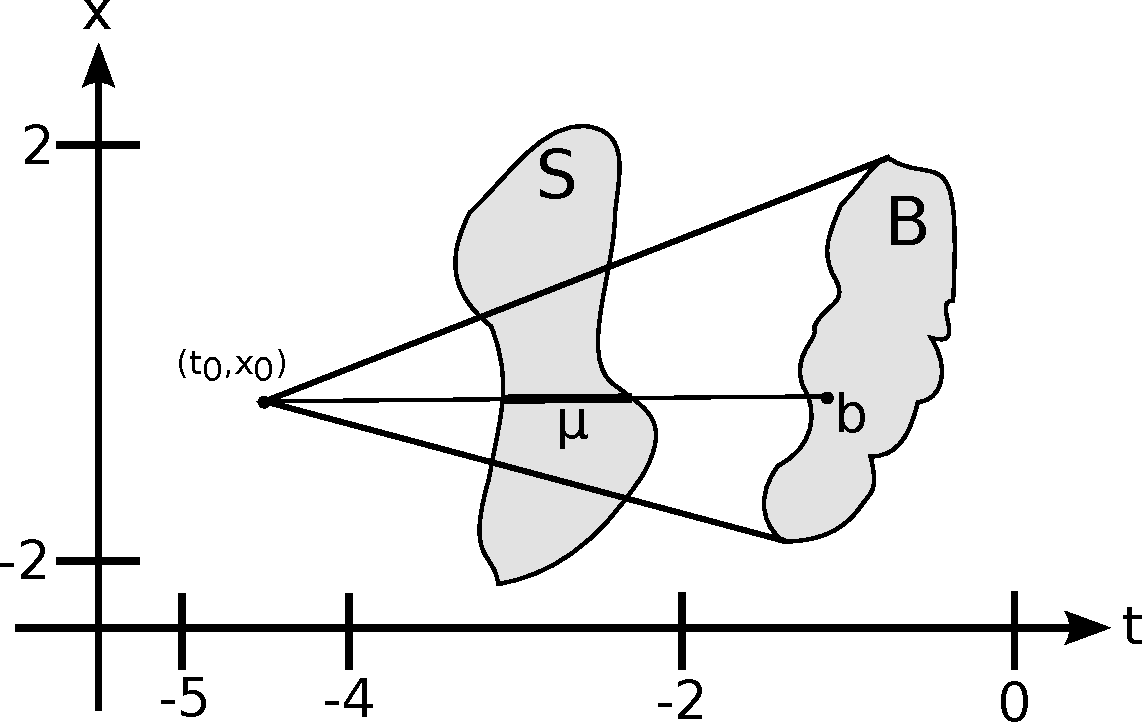
\includegraphics[width=.5 \textwidth]{NFP-diagram-Cone}
\caption{A diagram showing the assumptions of Lemma~\ref{thm:cone}.}
\end{figure}

\begin{lemma}\label{thm:cone}
Let $\mathcal{C} \subseteq \R \times \R^n$ be a cone from a vertex $(t_0,x_0) \in [-5, -4] \times B_2$ to a base set $B \subseteq [-2,0]\times B_2$.  % having $(t_0,x_0) \in [-5, -4] \times B_2$ and $B \subseteq [-2,0]\times B_2$.  
Let $S$ be a subset of $\R\times\R^n$ such that for each $b \in B$, the line segment connecting $(t_0,x_0)$ to $b$ intersects $S$ on a set with Hausdorff $\mathcal{H}^1$ measure at least $\mu$.  

Then 
\[ \abs{\mathcal{C} \cap S} \geq \frac{ |B| \mu^2}{80}. \]
\end{lemma}

\begin{proof}
Let $A(t)$ be the cross-sectional area of our cone at time slice $t$.  If $\mathcal{H}^n$ is the Hausdorff measure of dimension $n$, we write
\[ A(t) = \mathcal{H}^n\paren{\mathcal{C} \cap \bracket{\{t\}\times \R^n}}. \]
By the nature of cones, $A(t_0)=0$, $A$ is affine for $t_0 < t < -2$, then sub-affine for $-2<t<0$, and $A(t)=0$ for $t > 0$.  Specifically,
\[ A(t) = \frac{A(-2)}{-2-t_0} \paren{t-t_0} \qquad t_0 < t < -2, \]
\[ A(t) \leq \frac{A(-2)}{-2-t_0} \paren{t-t_0} \qquad -2 \leq t. \]


Since $B$ is contained in $\mathcal{C} \cap [-2,0]\times \R^n$, 
\[ |B| \leq \int_{-2}^0 A(t) \,dt \leq \int_{-2}^0 \frac{A(-2)}{-2-t_0}\paren{t-t_0} \,dt = \frac{A(-2)}{-2-t_0} \bracket{t_0^2 - (2+t_0)^2}/2 \leq 4 A(-2). \]

This means that 
\[ A(-2) \geq \frac{|B|}{4}. \]

Now we have a lower bound on the size of the cone, so for $t_0 \leq t \leq -2$
\begin{equation}\label{lower_bound_on_A} 
A(t) \geq \frac{|B|}{4(-2-t_0)}(t - t_0). 
\end{equation}

%Since $A(t)$ is increasing in $t$, the total measure of $\mathcal{C}\cap S$ will be smallest when $S$ is located near the vertex.  Each segment intersects $S$ on a set with measure at least $\mu$, and a segment of length $\mu$ can fit inside the cylinder $[t_0,t_0+x]\times B_2$ $\mu^2 = 4^2 + x^2$, $x = \sqrt{\mu^2 - 16}$.  At its most slant, a segment goes up $-2-t_0$ and over $4$, so with an extent $t$ you get rise $t$ and run $4t/(-2-t_0)$ for a length$^2$ of $t^2 + 16t^2/(2+t_0)^2$ or $t^2 \paren{1 + 16/2^2} = 5t^2$.  
%
%Consider a point $b \in B$ and the line segment from $(t_0,x_0)$ to $b$, which intersects $S$ on a set of measure at least $\mu$.  Because $A(t)$ is increasing in $t$, this intersection contributes more 

Consider the map from $B$ to $\{0\}\times\R^n$ given by stereographic projection from the point $(t_0,x_0)$, and let $db$ be a probability measure on $B$ proportional to the pullback of $\mathcal{H}^n \rest_{\{0\}\times\R^n}$ under this projection.  %In other words, $db(E)$ is the probabilty that a ray from $(t_0,x_0)$ to $B$ will intersect $E$.  
%Let $db$ be a probability measure on $B \subseteq \R \times \R^n$ which is a pullback of the stereographic projection, with pole $(t_0,x_0)$, from $\R \times \R^n$ to a copy of $\R^n$.  It measures what percentage of the rays from $(t_0,x_0)$ intersect a region of $B$.  
Then $db$ represents the proportion of any time-slice of $\mathcal{C}$ generated by rays through a given portion of $B$.  

To find the measure of $\mathcal{C} \cap S$, we must ask how much each time slice intersects $S$, or in integral form
\[ \abs{\mathcal{C} \cap S} = \int_{t_0}^{0} A(t) \int_{b \in B} \indic{(t,x) \in \mathcal{C} \cap S} \,dbdt. \]
By Fubini, this becomes
\begin{equation}\label{measure_of_intersection} 
\abs{\mathcal{C} \cap S} = \int_{b \in B} \int_{t_0}^0 A(t) \indic{(t,x) \in \mathcal{C} \cap S} \,dtdb. 
\end{equation}

From the definition of $\mu$ and the arc length formula,
\[ \mu \leq \int_{t_0}^0 \indic{(t,x) \in \mathcal{C} \cap S} \sqrt{1 + |b-x_0|^2/(-2-t_0)^2} \,dt \leq \sqrt{5} \int_{t_0}^0 \indic{(t,x) \in \mathcal{C} \cap S}. \]

Because $A(t)$ is increasing and $\indic{(t,x) \in \mathcal{C} \cap S}$ integrates to at least $\mu/\sqrt{5}$, 
\[ \int_{t_0}^0 A(t) \indic{(t,x) \in \mathcal{C} \cap S} \,dt \geq \int_{t_0}^{t+\mu/\sqrt{5}} A(t) \,dt. \]
From this bound, \eqref{measure_of_intersection}, and \eqref{lower_bound_on_A} we can at last compute
\[ \abs{\mathcal{C} \cap S} \geq \frac{|B|}{4(-2-t_0)} \int_{t_0}^{t_0 + \mu/\sqrt{5}} (t-t_0) \,dt = \frac{|B|}{4(-2-t_0)} \frac{\mu^2}{10} \geq \frac{|B|\mu^2}{80}. \]
\end{proof}

The following lemma is a commonly known fact about mollifiers.  Despite being known, a proof is surprisingly difficult to find in the existing literature.  Therefore, in the interest of completeness, we prove it here.   

\begin{lemma}\label{thm:convolution_estimate}
Let $\eta\in \Ctest(\R^n)$ be such that the sequence $\eta_\eps(v) = \eps^{-n} \eta(v/\eps)$ is an approximation to the identity.  There exists a constant $C=C(n,s,\eta)$ such that, for any $g \in H^s(\R^n)$, 
\[ \norm{g - g\ast \eta_\eps}_{L^2(\R^n)} \leq C \norm{g}_{H^s(\R^n)} \eps^s. \]
\end{lemma}

\begin{proof}
The bound is easy to compute by taking the Fourier transform and using Plancharel's theorem:
\begin{align*} 
\norm{g - g\ast \eta_\eps}_{L^2}^2 &= \int \hat{g}^2 \paren{1 - \hat{\eta_\eps}}^2 \,d\xi 
\\ &\leq \int (1+\xi^2)^s \hat{g}^2 \,d\xi \,\, \sup_{\xi} \frac{\abs{1-\hat{\eta_\eps}(\xi)}^2}{(1+\xi^2)^s}
\\ &= \norm{g}_{H^s(\R^n)}^2 \,\, \sup_{\xi} \frac{\abs{1-\hat{\eta_\eps}(\xi)}^2}{(1+\xi^2)^s}.
\end{align*}

Since $\eta \in \Ctest$, the fourier transform $\hat{\eta}$ is Lipschitz with some constant $\bar{C}$. Thus $\hat{\eta_\eps}(\xi) = \hat{\eta}(\eps \xi)$ is Lipschitz with constant $\bar{C}\eps$.  Since $\eta_\eps$ is an approximation to the identity, $\hat{\eta_\eps}(0) = 1$ and $\abs{\hat{\eta_\eps}(\xi)} \leq 1$ for all $\xi$.  Thus
\[ \abs{1 - \hat{\eta_\eps}(\xi)} \leq \min(2,\bar{C}\eps|\xi|). \]
%
%Our goal is to bound
%\begin{align*} 
%\norm{g - g\ast \eta_\eps}_{L^2}^2 &= \int \hat{g}^2 \paren{1 - \hat{\eta_\eps}}^2 \,d\xi 
%\\ &\leq \int (1+\xi^2)^s \hat{g}^2 \frac{\min(2,C\eps|\xi|)^2}{(1+\xi^2)^s} \,d\xi. 
%\end{align*}

The function $\frac{\min(2,\bar{C}\eps\xi)^2}{(1+\xi^2)^s}$ achieves its maxumum value at the critical point $\bar{C}\eps|\xi| = 2$, and that maximum value is 
\[ \frac{2^2}{\paren{1+\paren{\frac{2}{\bar{C}\eps}}^2}^s} = \frac{4 \eps^{2s}}{\paren{\eps^2 + 4/\bar{C}^2}^s} \leq C \eps^{2s}. \]
\end{proof}


%-----------------------------------------------------------------------------
%-----------------------------------------------------------------------------
%-----------------------------------------------------------------------------


\section{Technical Lemmas for Chapter \ref{ch:SQG}} \label{sec:technical}

In this appendix we state and prove a few technical lemmas.  

\begin{lemma}[De Giorgi Iteration Argument] \label{thm:DG1 skeleton}
For any constant $\bar{C} \geq 0$, there exists a $\delta>0$ such that the following holds:

Let $\Omega \subseteq \R^2$ be a bounded open set with $C^{2,\beta}$ boundary for some $\beta \in (0,1)$.  
Let $f \in L^2([-2,0]\times\Omega)$ be a function with the property that for any positive constant $a$
\begin{equation} \label{DG energy ddt} \ddt \int (f-a)_+^2 + \int \abs{\Lambda^{1/2} (f-a)_+}^2 \leq \bar{C} \paren{ \int \indic{f \geq a} + \int (f-a)_+ + \int (f-a)_+^2 }. \end{equation}

Then
\[ \int_{-2}^0 \int (f-0)_+^2 \,dxdt \leq \delta \]
implies that
\[ f(t,x) \leq 1 \qquad \forall t\in[-1,0], x \in \Omega. \]
\end{lemma}

\begin{proof}
Consider for $k \in \N$ the constants $t_k := -1 - 2^{-k}$ (so that $t_0 = -2$ and $t_\infty = -1$), and functions
\[ f_k := (f - 1 + 2^{-k})_+ \]
(so that $f_0 = (f)_+$ and $f_\infty = (f-1)_+$).  

Define
\[ \E_k := \int_{t_k}^0 \int_\Omega f_k^2 \,dxdt. \]

When $f_{k+1}>0$, then in particular $f_k \geq 2^{-k-1}$.  Thus for any finite $p$, there exists a constant $C$ so
\begin{equation} \label{non-linearization} \indic{f_{k+1}>0} \leq C^k f_k^p. \end{equation}
\vskip.3cm

Let $k\geq 0$ and define $\eta:[-2,0] \to \R$ a continuous function
\[ \eta(t) := \begin{cases}
0 & t \leq t_k \\
2^{k+1} (t-t_k) & t_k \leq t \leq t_{k+1} \\
1 & t_{k+1} \leq t.
\end{cases} \]

Let $s \in (t_{k+1},0)$.  Multiplying the inequality \eqref{DG energy ddt} with cutoff $a_k$ by $\eta(t)$ and integrating in time from $-2$ to $s$, then integrating by parts, we obtain
\[ \int f_k(s,x)^2\,dx - 2^{k+1} \int\displaylimits_{t_k}^{t_{k+1}} \int f_k(t,x)^2 \,dxdt + \int\displaylimits_{t_{k+1}}^s \HDint{1/2}{f_k} \,dxdt \leq \bar{C} \paren{ \int\displaylimits_{t_k}^0 \int \indic{f_k>0} + f_k + f_k^2 \,dxdt } \]
By taking the supremum over all $s \in (t_{k+1},0)$, we obtain
\begin{equation} \label{DG energy sup}
\sup_{[t_{k+1},0]} \int f_k^2 \,dx + \int_{t_{k+1}}^0 \HDint{1/2}{f_k}\,dxdt \leq C \paren{ 2^{k+1} \int_{t_k}^0 \int f_k^2\,dxdt + \int_{t_k}^0 \int \indic{f_k > 0} + f_k \,dxdt } 
\end{equation}
\vskip.3cm

From Proposition~\ref{thm:hadamard 3 lines} and Sobolev embedding, 
\[ \int_{t_{k+1}}^0 \paren{ \int f_k^4 \,dx }^{1/2} \,dt \leq C \int_{t_{k+1}}^0 \HDint{1/2}{f_k} \,dxdt. \]
Therefore by the Riesz-Thorin interpolation theorem,
\[ \int_{t_{k+1}}^0 \int f_k^3 \,dxdt \leq C \paren{ \sup_{[t_{k+1},0]} \int f_k^2 \,dx + \int_{t_{k+1}}^0 \HDint{1/2}{f_k} }^{3/2}. \]
This estimate, along with \eqref{DG energy sup} and \eqref{non-linearization}, and the fact that $t_{k-1} < t_k$ and $f_{k-1} \geq f_k$, tell us that
\[ \int_{t_{k+1}}^0 \int f_k^3 \,dxdt \leq C^k \E_{k-1}^{3/2}. \]

Now we can estimate, using again \eqref{non-linearization} and the fact $f_k \geq f_{k+1}$,
\[ \E_{k+1} \leq C^k \int_{t_{k+1}}^0 \int f_k^3 \,dxdt \leq C^k \E_{k-1}^{3/2}. \]
\vskip.3cm

This nonlinear recursive inequality $\E_{k+1} \leq C^k \E_{k-1}^{3/2}$, by a standard fact about nonlinear recursions (see \cite{DG} or \cite{Va.dg}), tells us that there exists a constant $\delta$ depending only on $C$ (which in turn depends only on the constant $\bar{C}$ in \eqref{DG energy ddt})
\[ \E_0 \leq \delta \textrm{ implies } \lim_{k \to \infty} \E_k = 0. \]

By assumption
\[ \E_0 = \int_{-2}^0 \int (f)_+ \leq \delta. \]
Therefore $\E_k \to 0$ and, by the dominated convergence theorem,
\[ \int_{-1}^0 \int (f-1)_+ \,dxdt = 0. \]

The result follows.  
\end{proof}

%\label{thm:Holder interpolation}

\begin{lemma} \label{thm:interpolation C1 to holder}
Let $\alpha \in (0,1)$.  There exists a constant $C = C(\alpha)$ such that, for any set $\Omega$ and any $f \in C^{0,1}(\Omega)$,
\[ \bracket{f}_\alpha \leq C \norm{f}_\infty^{1-\alpha} \norm{\grad f}_\infty^\alpha. \]
\end{lemma}

\begin{proof}
This simple lemma is a straightforward calculation:
\begin{align*} 
\sup_{x,y \in \Omega} \frac{|f(x)-f(y)|}{|x-y|^\alpha} &= \sup |f(x)-f(y)|^{1-\alpha} \paren{\frac{|f(x)-f(y)|}{|x-y|}}^\alpha 
\\ &\leq \paren{2 \norm{f}_\infty}^{1-\alpha} \paren{ \sup \frac{|f(x)-f(y)|}{|x-y|} }^\alpha
\\ &\leq C \norm{f}_\infty^{1-\alpha} \norm{\grad f}_\infty^\alpha.
\end{align*}
\end{proof}

\begin{lemma} \label{thm:interpolation holder to C1}
Let $\alpha \in (0,1)$ and $\Omega$ a set that satisfies the cone condition.  There exist constants $C = C(\alpha, \Omega)$ and $\ell = \ell(\Omega)$ such that, for any $f \in C^{1,\alpha}(\Omega)$
\[ \norm{\grad f}_\infty \leq C \paren{ \delta\n \norm{f}_\infty  + \delta^\alpha \bracket{\grad f}_\alpha }\]
for all $\delta < \ell$.  
\end{lemma}

The idea of the proof is to average $\grad f$ along an interval of length $\delta$ with endpoint $x$.  The magnitude of the average will be small, since $f \in L^\infty$, and the average will differ not very much from $\grad f(x)$ since $\grad f \in C^{1,\alpha}$.  

\begin{proof}
Since $\Omega$ satisfies the cone condition, there exist positive constants $\ell$ and $a<1$ such that, at each point $x \in \bar{\Omega}$, there exist two unit vectors $e_1$ and $e_2$ such that $|e_1\cdot e_2| \leq a$ and $x + \tau e_i \in \Omega$ for $i=1,2$ and $0 < \tau \leq \ell$.  In other words, $\Omega$ contains rays at each point that extend for length $\ell$, end at $x$, and are non-parallel with angle at least $\cos\n(a)$.  

Consider the directional derivative $\del_i f$ of $f$ along the direction $e_i$, and observe that for any $0 < \delta \leq \ell$,
\begin{equation} \label{average bounded by Linfty} \abs{\int_0^\delta \del_i f(x + \tau e_i) \,d\tau} = \abs{f(x+\delta e_i) - f(x)} \leq 2 \norm{f}_\infty. \end{equation}

On the other hand, $\del_i f$ is continous so, for any $\tau \in (0,\ell]$,
\[ \abs{\del_i f(x) - \del_i f(x+\tau e_i)} \leq \bracket{\grad f}_\alpha \tau^\alpha. \]
From this, we obtain that
\[ \int_0^\delta \del_i f(x + \tau e_i) \,d\tau \leq \int_0^\delta \paren{\del_i f(x) + \bracket{\grad f}_\alpha \tau^\alpha } \,d\tau = \delta \del_i f(x) + \bracket{\grad f}_\alpha \frac{\delta^{1+\alpha}}{1+\alpha} \]
and a similar bound holds from below.  Thus
\[ \abs{ \delta \del_i f(x) - \int_0^\delta \del_i f(x + \tau e_i) \,d\tau} \leq \bracket{\grad f}_\alpha \frac{\delta^{1+\alpha}}{1+\alpha}. \]

Combining this bound with \eqref{average bounded by Linfty}, we obtain
\[ \abs{\del_i f(x)} \leq \frac{2}{\delta} \norm{f}_\infty + \frac{\delta^\alpha}{1+\alpha} \bracket{\grad f}_\alpha. \]

This bound is independent of $x$ and of $i=1,2$.  Since $e_1 \cdot e_2 \leq a$ by assumption, by a little linear algebra we can bound $\grad f$ in terms of the $\del_i f$ and obtain that, for all $\delta \in (0,\ell]$,
\[ \norm{\grad f}_\infty \leq \frac{C}{1-a^2} \paren{ \delta\n \norm{f}_\infty + \delta^\alpha \bracket{\grad f}_\alpha }. \]

\end{proof}



\begin{lemma} \label{thm:technical scaling of barrier}
There exist constants $\bar{\lambda} > 0$ and $\alpha > 1$ such that, for any $0 < \eps \leq 1/2$ and any $z \geq 1$
\[ \paren{|\eps\n (z - 1) + 3|^{1/4} - 2^{1/4}}_+ - \alpha \paren{|z|^{1/4} - 2^{1/4}}_+ \geq \bar{\lambda}. \]
\end{lemma}

\begin{proof}
For $z$ fixed, this function is increasing as $\eps$ decreases, so it will suffice to show the lemma when $\eps = 1/2$, that is to show
\[ f_\alpha(z) := \paren{|2 z + 1|^{1/4} - 2^{1/4}}_+ - \alpha \paren{|z|^{1/4} - 2^{1/4}}_+ \geq \bar{\lambda} \]
for all $z \geq 1$.  Note that $f_\alpha(z) \geq f_\beta(z)$ if $\alpha < \beta$.  

For $z \geq 2$, 
\[ f_\alpha(z) = (2z+1)^{1/4} - 2^{1/4} - \alpha z^{1/4} + \alpha 2^{1/4} = z^{1/4} \paren{(2 + 1/z)^{1/4} - \alpha} + (\alpha-1)2^{1/4}. \]
For any $\alpha < 2^{1/4}$, clearly $f_\alpha(z)$ tends to $\infty$ as $z$ increases. Therefore there exist $N$ and $\alpha_0 > 1$ such that 
\[ f_\alpha(z) \geq 1 \qquad \forall z \geq N, \alpha\leq \alpha_0. \]
\vskip.3cm

We can decompose $f_\alpha(z) = g_1(z) - (\alpha - 1) g_2(z)$ where
\begin{align*} 
g_1(z) &:= \paren{|2 z + 1|^{1/4} - 2^{1/4}}_+ - \paren{|z|^{1/4} - 2^{1/4}}_+, \\
g_2(z) &:= \paren{|z|^{1/4} - 2^{1/4}}_+. 
\end{align*}
Note that $g_1$, $g_2$ are both continuous, and $g_1(z)$ is strictly positive for $z \geq 1$.  Therefore we can take $\alpha \in (1,\alpha_0]$ small enough that
\[ \alpha - 1 < \frac{\inf_{[1,N]} g_1}{\sup_{[1,N]} g_2}. \]

For this $\alpha$, $f_\alpha(z)$ is strictly positive on the compact interval $[1,N]$, and $f_\alpha(z) \geq 1$ on $[N,\infty)$.  Therefore $f_\alpha(z)$ has a positive lower bound $\bar{\lambda}$ for all $z \geq 1$.  
\end{proof}
%
%\include{chapter-appendix2}
%
%\include{chapter-appendix3}


%%%%%%%%%%%%%%%%%%%%%%%%%%%%%%%%%%%%%%%%%%%%%%%%%%%%%%%%%%%%%%%%%%%%%%
% Generate the bibliography.					     %
%%%%%%%%%%%%%%%%%%%%%%%%%%%%%%%%%%%%%%%%%%%%%%%%%%%%%%%%%%%%%%%%%%%%%%
%\nocite{*}      % This command causes all items in the 		
                % bibliographic database to be added to 	  
                % the bibliography, even if they are not 	  
                % explicitly cited in the text. 		     

\bibliographystyle{alpha}
\bibliography{StokolsThesis}
%\index{Bibliography@\emph{Bibliography}}%			     %
%%%%%%%%%%%%%%%%%%%%%%%%%%%%%%%%%%%%%%%%%%%%%%%%%%%%%%%%%%%%%%%%%%%%%%


%%%%%%%%%%%%%%%%%%%%%%%%%%%%%%%%%%%%%%%%%%%%%%%%%%%%%%%%%%%%%%%%%%%%%%
% Generate the index.						     %
%%%%%%%%%%%%%%%%%%%%%%%%%%%%%%%%%%%%%%%%%%%%%%%%%%%%%%%%%%%%%%%%%%%%%%
%								     %
% NOTE: For master's theses and reports, NOTHING is permitted to     %
%	come between the bibliography and the vita. This section     %
%	to generate the index (if used) MUST be moved to before      %
%	the bibliography section.				     %
%								     %
%\printindex%    % Include the index here. Comment out this line      %
%		% with a percent sign if you do not want an index.   %
%%%%%%%%%%%%%%%%%%%%%%%%%%%%%%%%%%%%%%%%%%%%%%%%%%%%%%%%%%%%%%%%%%%%%%


%%%%%%%%%%%%%%%%%%%%%%%%%%%%%%%%%%%%%%%%%%%%%%%%%%%%%%%%%%%%%%%%%%%%%%
% Vita page.							     %
%%%%%%%%%%%%%%%%%%%%%%%%%%%%%%%%%%%%%%%%%%%%%%%%%%%%%%%%%%%%%%%%%%%%%%

%\begin{vita}
%Craig William McCluskey
%was born in Minneapolis, Minnesota on 20 May 1950, the son of
%Dr. William R. McCluskey and Lucilla W. McCluskey.  He received the Bachelor
%of Science degree in Engineering from the California Institute of Technology
%and was commissioned an Officer in the United States Air Force in 1971.
%He entered active duty in October, 1971, and was stationed in Denver, Colorado,
%Colorado Springs, Colorado, Panama City, Florida, and Sacramento, California.
%He separated from the USAF in 1975 and worked as an engineer for several small
%electronics companies in California before moving to Colorado Springs, Colorado
%to work for Hewlett-Packard in 1979. He left Hewlett-Packard in 1989 and joined
%a small company based in Herndon, Virginia, working out of his house as a
%``remote'' engineer designing parts of the Alexis satellite for Los Alamos
%National Laboratories. Laid off when his portion of the satellite was
%completed, he applied to the University of Texas at Austin for enrollment
%in their physics program. He was accepted and started graduate studies in
%August, 1991.
%
%\end{vita}

\end{document}
